\documentclass[12pt,epsfig,color,russian]{book}
\usepackage[russian]{babel}
\usepackage{epsfig}
\usepackage{color}
\usepackage{hyperref}
\usepackage{caption}
\usepackage[normalem]{ulem}

% Преамбула
\title{Общая физика}
\author{Егоров Вячеслав Георгиевич}
\date{\today} % Дата создания или любая другая дата

\begin{document}

\begin{titlepage}
    \centering
    \vspace*{\stretch{1}} % Добавляет вертикальное пространство перед изображением
    
    % Название книги
    {\Huge\bfseries Лекции по общей физике\par}
    \vspace{1.5cm}
    
    % Автор(ы)
    {\Large Егоров Вячеслав Георгиевич\par}
    \vspace{2cm}
    
    % Вставка изображения
    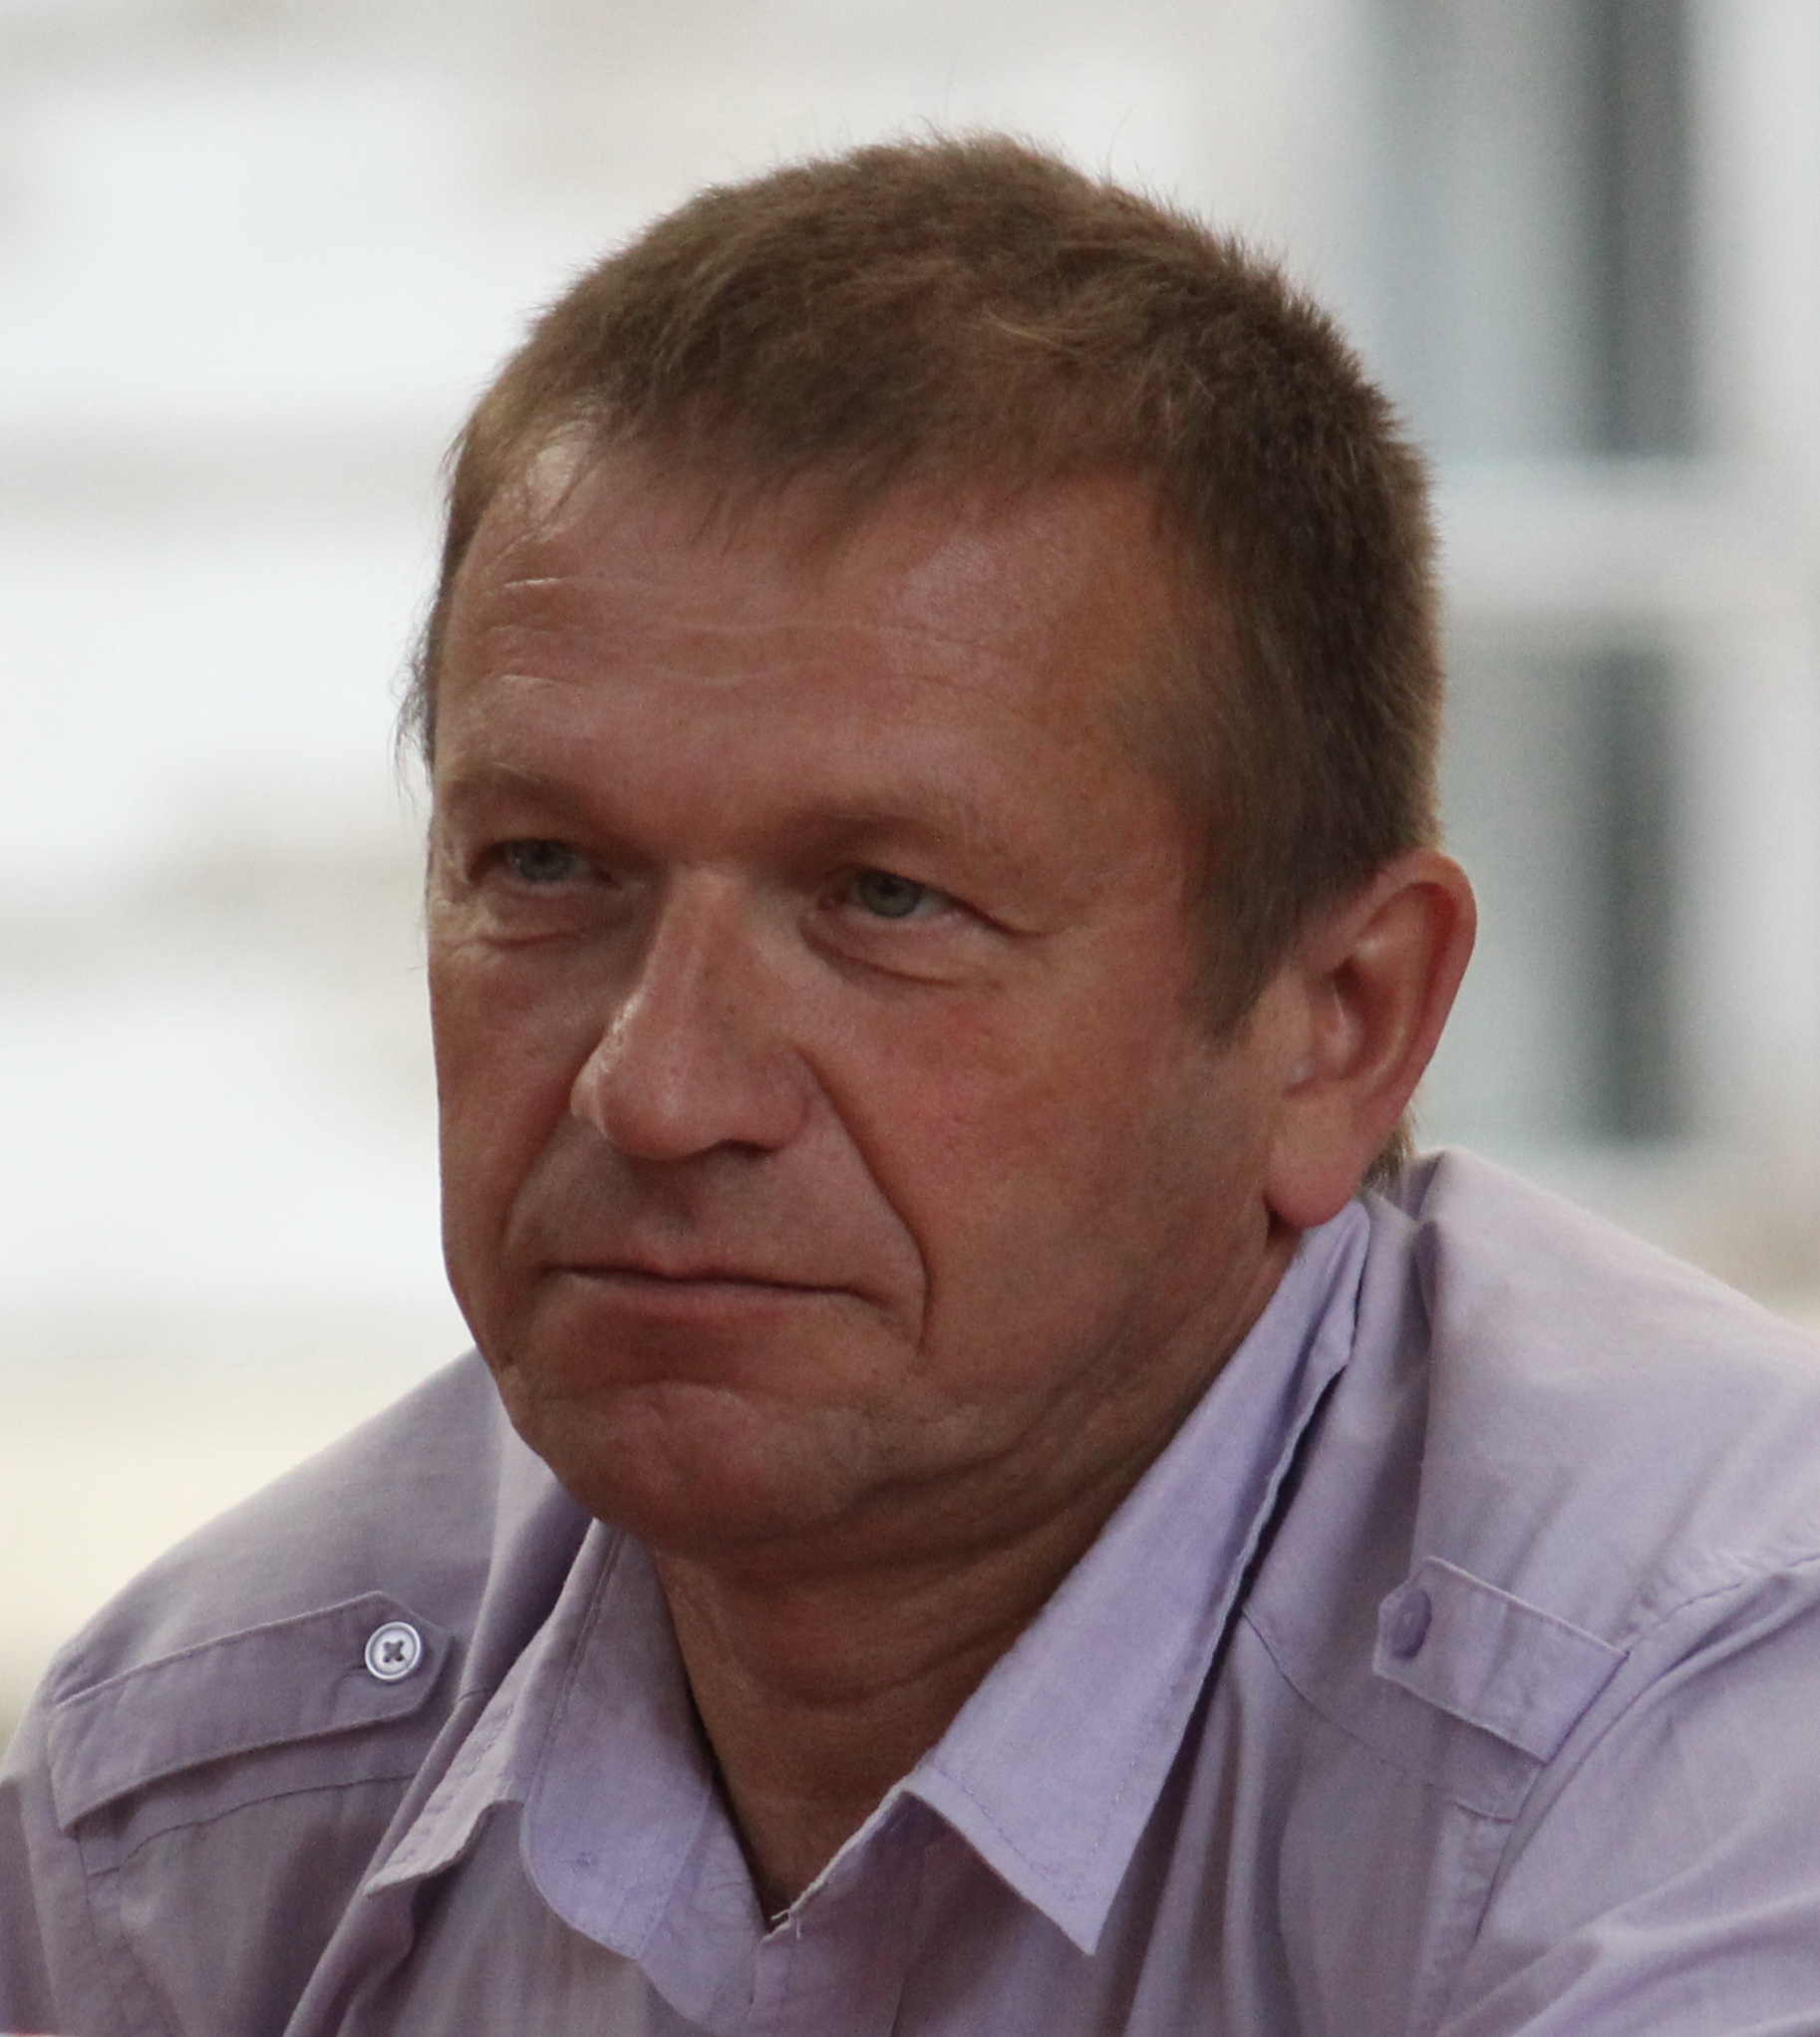
\includegraphics[width=0.8\textwidth]{photos/Egorov.jpg}
 %   \vspace{3cm}
    
    % Дополнительная информация
  %  {\large Дополнительная информация\par}
    
 %   \vspace*{\stretch{2}} % Добавляет вертикальное пространство после изображения
\end{titlepage}

%\maketitle % Создает титульную страницу с указанными выше заголовком, автором и датой

\frontmatter
% Здесь может идти содержание, предисловие, благодарности и т.д.

% Adding table of contents
\tableofcontents
\newpage

\chapter{Введение}
% Текст введения	
Перед Вами – необычное издание. Это лекции \href{https://dlnp.jinr.ru/news/618}{Егорова Вячеслава Георгиевича} по общей физике, которые он читал студентам \href{https://www.uni-dubna.ru/}{университета «Дубна»}.

Доктор физико-математических наук, начальник сектора отдела НЭОЯСиРХ ОИЯИ, профессор кафедры физики университета «Дубна» Егоров Вячеслав Георгиевич был выдающимся физиком, представителем того редкого и почти исчезнувшего вида ученых, которые способны самостоятельно выполнить физический эксперимент от начала и до конца. От идеи, поставновки задачи через создание установки к проведению измерений и завершая анализом данных, получением результатов и написанием статьи. Нужно отметить, что в современной науки чаще всего существует явная специализация, есть эксперты по электронике, написанию ПО, симуляциям, обработке данных. Безусловно, этому способствует неизбежная глобализация в науке – все ведущие направления исследований требуют создания огромных установок – научных фабрик, в которых заняты сотни и тысячи ученых. Тот же Слава говорил «все простые законы, которые лежали, уже давно расхватали. Это раньше можно было взять магнит и проволоку, открыть закон, назвав его своим именем. А теперь нужно сильно напрягаться и копать глубоко». Но, все равно, универсализм и умение мастеров на все руки все еще вызывает истинное восхищение и уважение.

И второй важный момент, имеющий прямое отношение к данной книге – Слава был Учителем с большой буквы, он всегда умел объяснить сложные вещи простыми словами, находить удачные и точные образы, проявляя при этом удивительную находчивость и смекалку. Способности Славы как нельзя лучше передает жизненная история, случившаяся с нами в большом французском супермаркете, где мы искали лавровый лист и никак не могли найти. Тогда Слава подозвал девушку-работника магазина и попытался поговорить с ней на английском. Но она его не поняла. Тогда Слава, недолго думая, взял в руки воображаемый лавровый венок, торжественно надел его себе на голову и стал в позу Наполеона. Девушка засмеялась и тут же отвела нас к стойке со специями.

Я сам не знал об этих лекциях, но услышал о них впервые от своего коллеги \href{https://www.utef.cvut.cz/staff/00078/ivan-stekl}{Ивана Штекла}, который после ухода Славы сказал «у Славы были отличные лекции по физике, которые жалко было бы потерять». И вот, разбирая электронные документы с его компьютера я наткнулся на папку lectures. Каждая лекция была в отдельной папке, в формате LaTeX, огромное количество оригинальных рисунков, формул – и это все было сделано вручную, до эпохи chatGPT и MidJourney… Тут понимаешь,что на это были потрачены десятки, если не сотни часов времени – Слава, как всегда, если брался за что-то, то делал это на совесть, а также с присущим ему страстью и энтузиазмом.

Лекции сохранены в практически оригинальном стиле автора, с небольшими техническими изменениями,  связаными с компоновкой в единую книгу. Несколько первых глав были отформатированы в универсальном стиле книги, но потом я бросил эту затею, потому что уникальный авторский стиль просто невозможно подогнать под стандарт. Во-первых, это потребует большого объема работы, во-вторых, это уже будет другой документ. Поэтому пусть все останется так, как было задумано и реализовано автором.

Это не обычный канонический фундаментальный курс общей физики, пытающийся охватить все темы подробно. Наоборот, это выжимка, дайджест, избранные главы, экстракт наиболее важных, по мнению автора, физических понятий, которые необходимо знать студенту. Это своеобразная \sout{книжка-комикс}, \sout{книжка-раскраска}, книжка-презентация с яркими картинками и интересными примерами. Уверен, что каждый найдет в ней что-то интересное. Студент может использовать для обучения. Специалист – может увидеть уже известные ему вещи с иной стороны, под иным углом зрения. Как та девушка, увидевшая Наполеона в лавровом венке...

Удачного прочтения!

{\bf Шитов Ю.А.}

\centering
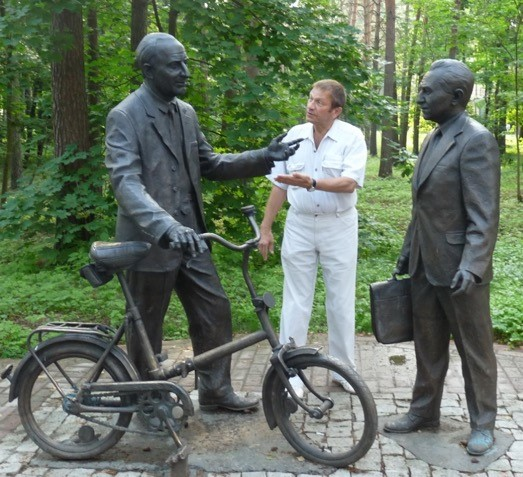
\includegraphics[width=0.9\textwidth]{photos/egorov_pontecorvo_djelepov.jpg}

Вячеслав Георгиевич обсуждае курс лекций по общей физике с Бруно Понтекорво и Венедиктом Петровичем Джелеповым.


\mainmatter
% Здесь начинается основное содержание книги

\chapter{Общий обзор,  план лекций и основные понятия}
%\begin{center}
%\huge\bf \underline{ФИЗИКА (Общая физика)}\\[5mm]
%\Large\sl Вячеслав Георгиевич ЕГОРОВ\\
%{\color{blue}(egorov@nusun.jinr.ru)}\\[10mm]
%\sf\LARGE
%2 семестра
%\end{center}

\section{Обзор (план) курса}
%\sf\LARGE
\begin{enumerate}
\item{\underline{\bf Физические основы механики}}

кинематика, динамика, понятие о работе и энергии, законы сохранения, силы тяготения, движение твердого тела и жид\-кости, основные положения СТО
\item{\underline{\bf Молекулярная физика}}

идеальный и реальный газы, распределения Максвелла и Больцмана, основы термодинамики, циклические процес\-сы, явление переноса, молекулярные явления в жидкостях и твердых телах

\item{\underline{\bf Колебания и волны}}

гармонический осциллятор, затухающие и вынужденные ко\-лебания, гармоники, гармонический анализ, волновые явле\-ния, принцип Гюйгенса, интерференция, дифракция, аку\-стические явления, фононы
\item{\underline{\bf	Электричество и магнетизм}}

электростатика, диэлектрики, законы постоянного тока, тер\-моэлектрические явления, ток в электролитах и газах, маг\-нитное поле тока, отклонение заряженных частиц в полях, индукция, электромагнитные колебания и волны

%\newpage
\item{\underline{\bf	Оптика}}

основные свойства света, волновая оптика (поляризация, интерференция и дифракция), прохождение света через ан\-изотропные и движущиеся вещества, голография, термоди\-намика излучения (световой поток, черное тело), лучевая оптика, фотоны

\item{\underline{\bf	Атомная физика}}

строение атомов и молекул, ионизация и диссоциация, боро\-вские орбиты, оптические переходы, правила отбора, спек\-троскопия, лазеры, лазерная спектроскопия, характеристи\-ческое рентгеновское излучение, рентгено-флуоресцентный анализ, масс-спектрометрия

\item{\underline{\bf	Ядерная физика}}

альфа-, бета-, гамма-процессы, ядерные реакции, взаимо\-действие излучений с веществом, детекторы ядерных излу\-чений, ядерные методы исследования материалов ("мече\-ные атомы", нейтроно-акти\-вационный анализ, ядерный ма\-гнитный резонанс)

\end{enumerate}

% \newpage
\section{Ошибки измерений}
 %\centerline{\underline{\huge\bf Ошибки %измерений}}\vspace{5mm}

 Абсолютные ($X =10\pm1$) и относительные ($\Delta X/X=10\%$)\vspace{4mm}

 Симметричные ($X =10\pm1$) и асимметричные ($X=10^{+2}_{-1}$)\vspace{4mm}

 Статистические (уменьшаются с ростом числа измерений) и \vspace{4mm}

 систематические (зависят от метода измерений)\vspace{4mm}

 Написание: 0.01234$\pm$0.00050 или 0.01234(50) или 0.01234$_{\it 50}$\vspace{4mm}

 Меряем 5 раз ширину стола: 1000, 1001, 999, 1000, 1001 мм.\vspace{5mm}

 Среднее значение:
 \begin{displaymath}
\overline{x} = \frac{1000 + 1001 + 999 + 1000 + 1001}{5} = 1000.2
 \end{displaymath}

 Дисперсия (разброс):
 \begin{displaymath}
\sigma \simeq \sqrt{\overline{\left( x_i-\overline{x} \right)^2}}
 \end{displaymath}
 \begin{displaymath}
(-0.2)^2 +(0.8)^2 + (-1.2)^2 + (-0.2)^2 + (0.8)^2 = 2.80
 \end{displaymath}
 \begin{displaymath}
\sigma \simeq \sqrt{(2.80/5)}=\sqrt{0.56} \simeq 0.75
 \end{displaymath}
 \begin{displaymath}
X = 1000.20\pm 0.75 \;\;(67\%CL)
 \end{displaymath}

Смысл дисперсии: с вероятностью 67\% каждое следующее измерение будет попадать в диапазон от 999.45 до 1000.95. Можно показать, что при большой статистике
\begin{displaymath}
X = \overline{x}\pm 2\sigma \;\;(95\%CL)\;\;\;\;\;\;X = \overline{x}\pm 3\sigma \;\;(99.7\%CL)
 \end{displaymath}

Если измерения имеют разную погрешность: 1000$\pm10$, 1001$\pm1$, 999$\pm1$, 1000$\pm1$ и 1001.0$\pm0.1$, то ищем \underline{среднее взвешенное}. \\
Вес i-ой точки: $p_i = \left(\Delta x_i\right)^{-2}$. Чем точнее -- тем больше вес.  Таким образом, веса равны 0.01, 1, 1, 1 и 100.
 \begin{displaymath}
\overline{X}=\frac{\sum_i p_ix_i}{\sum_i p_i}=1000.97;\;\;\;\;\;
\sigma=\sqrt{\frac{\sum_i p_i\left(x_i-\overline{x}\right)^2}{\sum_i p_i}}=0.22
 \end{displaymath}
%\newpage

Измеряем энергию $\gamma$-линии 1460.822(6) кэВ $^{40}$K (Рис.~\ref{fig:k40_spk}) с помощью HPGe детектора и АЦП со шкалой 1 кэВ на канал:

 \begin{figure}[ht]
\centering
 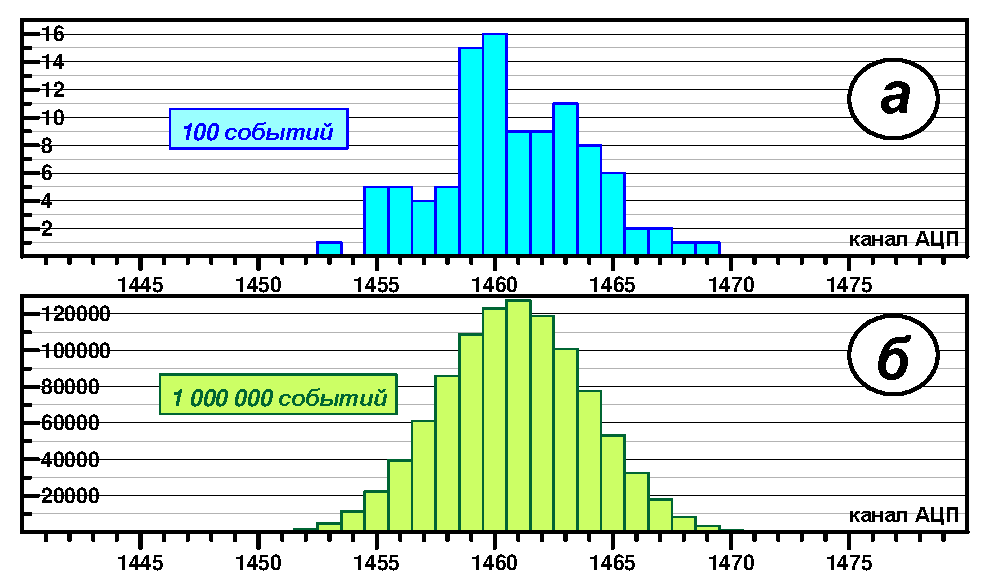
\includegraphics[width=0.95\textwidth]{GP001/GP001F01.eps}
 
% \begin{picture}(165,100)(0,0)
% \put(0, 0){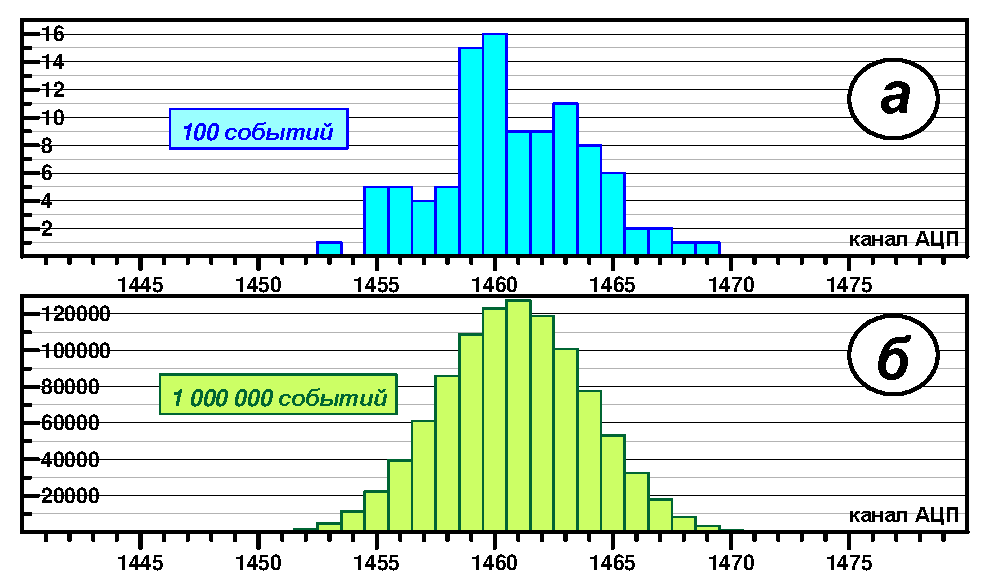
\includegraphics{GP001/GP001F01.eps}}
% \end{picture}
  \caption{Спектр $\gamma$-линии 1460.822(6) кэВ $^{40}$K, измеренной со статистикой 100 (а) и 1M (б) событий.}
   \label{fig:k40_spk} % Метка для ссылки на картинку
\end{figure}

 \begin{displaymath}
 \begin{array}{cclcll}
 a)&\hspace{5mm}&\overline{E} = \frac{1\cdot1453 + 5\cdot1455 +  \ldots
 + 1\cdot1469}{100}           & = 1460.76  &\hspace{5mm}&\sigma = 3.17\\
 b)&            &\overline{E} & = 1460.822 &            &\sigma = 3.066
 \end{array}
  \end{displaymath}

  Ошибка среднего значения:

 \begin{displaymath}
    \Delta(\overline{X}) = \overline{(\overline{X}-X_0)}\;\;\simeq\;\; \frac{\sigma}{\sqrt{N}}
 \end{displaymath}
 \begin{displaymath}
  \begin{array}{lclcl}
   \overline{E}_{(N=100)}     &=& 1460.76  & \pm & 0.32\\
   \overline{E}_{(N=1000000)} &=& 1460.822 & \pm & 0.003
  \end{array}
 \end{displaymath}
 
С увеличением статистики дисперсия не изменилась, но ошибка уменьшилась!
 \\[3mm]

\underline{Если измерение величины $\phi$ не прямое:} $\;\;\;\phi = f(x\pm\Delta x,y\pm \Delta y)$
 \begin{displaymath}
(\Delta\phi)^2 = \left(\frac{\partial f}{\partial x}\cdot\Delta x\right)^2 +
                 \left(\frac{\partial f}{\partial y}\cdot\Delta y\right)^2
 \end{displaymath}
(ошибка результата $\Delta\phi$)$^2$ = (ошибка из-за $\Delta x$)$^2$ + (ошибка из-за $\Delta y$)$^2$.\\ Производная $\frac{\partial f}{\partial x}$ -- это  {\em коэффициент влияния} параметра $x$ на функцию $f$.
%\newpage

\section{Метод Наименьших Кавдратов (Least Squares)}
%{\Huge Метод Наименьших Кавдратов (Least Squares)}\\[3mm]

Задача: фитировать набор N экспериментальных точек ($x_i,y_i$) какой-то
функцией $Y=f(X)$. LS-критерий -- малость остаточной суммы $\chi^2$.

 \begin{displaymath}
\chi^2 = \sum_{i=1}^N p_i\left[y_i - f(x_i)\right]^2;\;\;\;\;\;\;\;\;\;\;
p_i = \frac{1}{\left(\Delta y_i\right)^2}\;\;.
 \end{displaymath}
 
Примеры фитирующих функций с 1 или 2 параметрами показаны на Рис.~\ref{fig:fit_fun}.

 \begin{figure}[htp] 
 \setlength{\unitlength}{1mm}
 \begin{picture}(165,180)(0,0)
 \put(10, 0){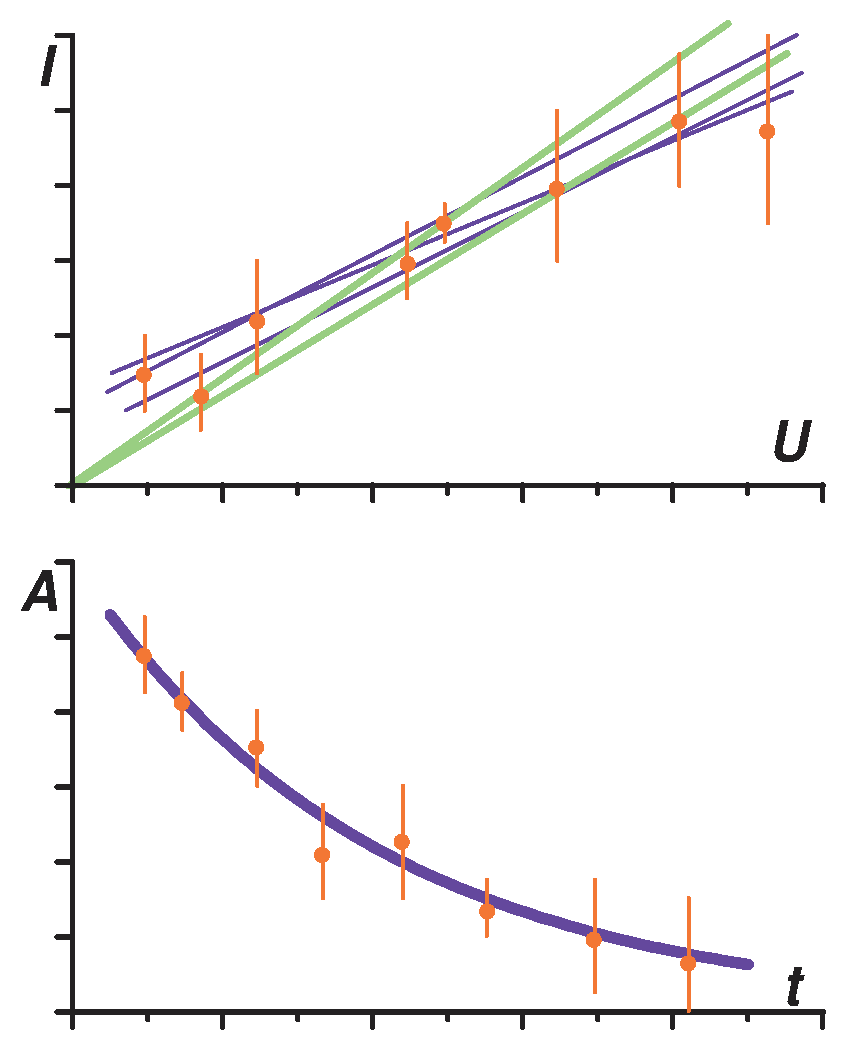
\includegraphics{GP001/GP001F02.eps}}
 \put(25, 165){\makebox(0,0)[l]{\Large\sf Вольт-амперная характеристика}}
 \put(48, 155){\makebox(0,0)[c]{\color{blue}\Huge\bf $I=aU+b$}}
 \put(22, 146){\makebox(0,0)[l]{\color{blue}\Large\bf (какая-то прямая,}}
 \put(22, 141){\makebox(0,0)[l]{\color{blue}\Large\bf надо найти $a$ и $b$)}}
 \put(120, 125){\makebox(0,0)[c]{\color{green}\Huge\bf $I=U/R=k\cdot U$}}
 \put(110, 115){\makebox(0,0)[c]{\color{green}\Large\bf (прямая проходит через О, }}
 \put(110, 109){\makebox(0,0)[c]{\color{green}\Large\bf надо найти наклон $k=1/R$)}}
 \put( 40,  70){\makebox(0,0)[l]{\Large\sf Закон радиоактивного распада}}
 \put(110,  57){\makebox(0,0)[c]{\color{blue}\Huge\bf $A=A_0\cdot e^{-t/\tau}$}}
 \put(105,  47){\makebox(0,0)[c]{\color{blue}\Large\bf (экспонента; надо найти $A_0$ и $\tau$)}}
 \end{picture}
\caption{Примеры фитирования вольт-амперной характеристики (вверху) и данных радиоактивного распада (внизу).}
   \label{fig:fit_fun} % Метка для ссылки на картинку
\end{figure}
 
%\newpage

Итак, надо найти такие значения двух параметров ($A_0$ и $\tau$), чтобы остаточная сумма $\chi^2$ была ми\-ни\-мальной. Условие минимума:

 \begin{displaymath}
\frac{\partial(\chi^2)}{\partial A_0}=0\;\;\;;\;\;\;\;\;\;
\frac{\partial(\chi^2)}{\partial \tau}=0\;\;.
 \end{displaymath}
 \begin{displaymath}
 \left\{
 \begin{array}{cc}
 \sum_i p_i \left[y_i-f(t_i)\right]\frac{\partial f(t_i)}{\partial A_0} &= 0\\[2mm]
 \sum_i p_i \left[y_i-f(t_i)\right]\frac{\partial f(t_i)}{\partial \tau} &= 0
 \end{array}
 \right|\;\;\;\;\;\;\Rightarrow\;\;\;A_0,\;\;\tau
 \end{displaymath}

Если сложный вид $f(x)$ и число параметров $K\gg 1$, то система не решается. Тогда используем \underline{топографический метод}: составляем как бы {\sl карту высот} $\chi^2$ на k-мерной плоскости и ищем на ней низину (Рис.~\ref{fig:2d_fit_surf}).

\begin{figure}[htp] 
 \setlength{\unitlength}{1mm}
 \begin{picture}(165,80)(0,0)
 \put(0, 0){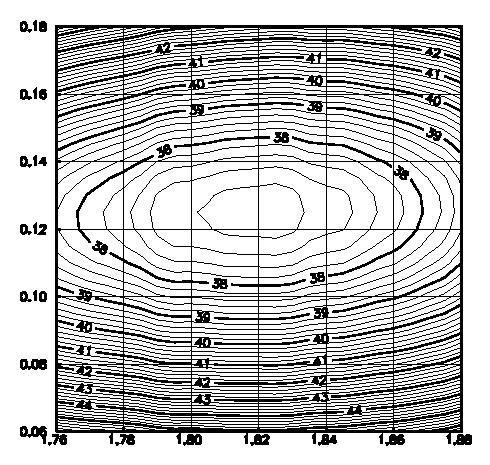
\includegraphics{GP001/GP001F03.eps}}
 \put(85, 0){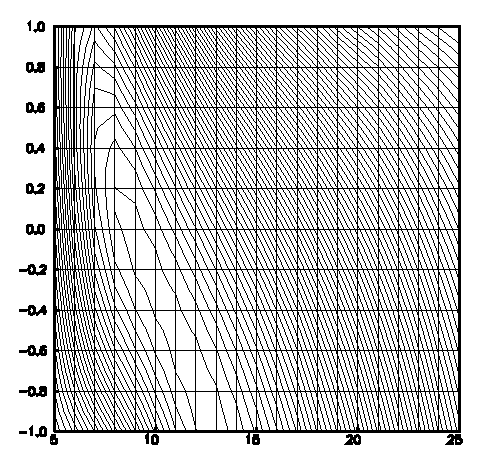
\includegraphics{GP001/GP001F04.eps}}
 {\color{red}
 \put(20,15){\vector(1,4){4}}
 \put(24,31){\vector(1,1){10}}
 \put(34,41){\vector(1,0){6}}
 \color{black}}
 \end{picture}
  \caption{2D-поверхности в фазовом пространстве фитируемых параметров.}
   \label{fig:2d_fit_surf} % Метка для ссылки на картинку
\end{figure}

\underline{Градиентный метод} (то же самое, но низина ищется автоматически). Суть: искомые параметры выбираются наугад (на k-мерной плоскости ставится точка), а затем для этой точки  ищется градиент, то есть, {\color{red}вектор}, показывающий на\-правление максимального изменения $\chi^2$. Находится новая точка, и т. д.  Стандартный программный пакет MINUIT.\\

Свойства  $\chi^2$
\begin{itemize}
\item если "покачать" параметр A на $\pm\Delta A$, то $\chi^2$ увеличится на +1.0
\item нормированное $\chi^2_{\rm norm}=\chi^2/(N-K)$ должно быть $\simeq1$.

Если $\chi^2_{\rm norm}>1$, то неверный вид функции или $\exists$ систематика.

Если $\chi^2_{\rm norm}<1$, то погрешность каждой точки слишком велика.
\end{itemize}
%\newpage

\section{Максимальное Правдоподобие (Maximal Likelyhood)}
%{\color{green}
%{\Huge Максимальное Правдоподобие (Maximal Likelyhood)}\\
%\underline{(Это -- пока вне программы; просто знайте, что %существует и такой метод)}
%}

Если в качестве фитируемых точек используется не измеренная каким-то прибором аналоговая величина $Y_i\pm\Delta Y_i$, а число событий $N_i(X)$ (например, число $\gamma$-квантов, зарегистрированных детектором), то как быть с погрешностью $\Delta N_i$ и весом точек? При больших $N$ погрешность
$\Delta N\simeq\sqrt{N}$, а при малых -- ?...

ML-критерий: надо так подобрать параметры фитирующей функции $f(x)$, чтобы была максимальной вероятность получить в эксперименте именно те точки, которые в нем и получились.

\begin{figure}[ht]
 \setlength{\unitlength}{1mm}
 \begin{picture}(165,90)(0,0)
 \put(0,5){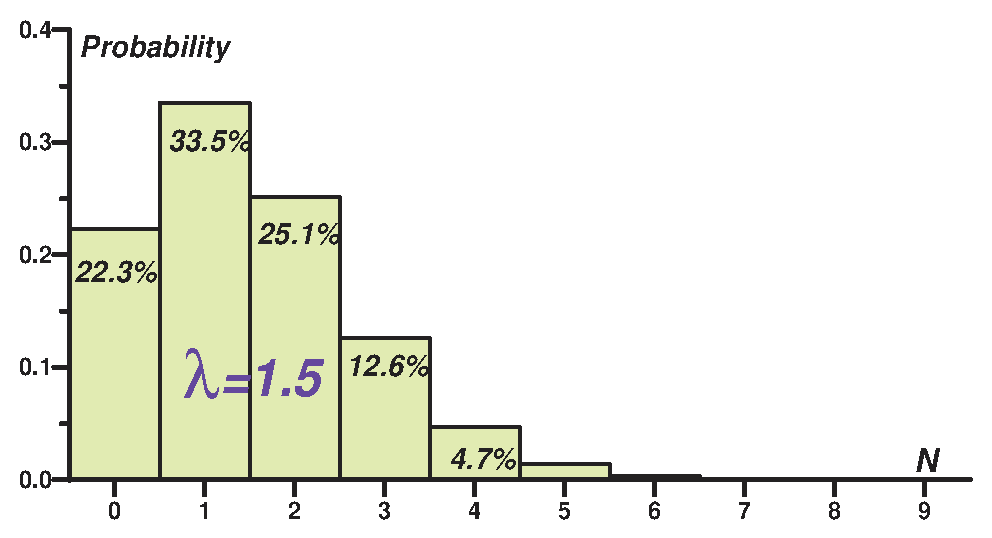
\includegraphics{GP001/GP001F05.eps}}
 \end{picture}
\caption{Распределение пуассона с параметрами задачи в тексте.}
   \label{fig:poisson} % Метка для ссылки на картинку
\end{figure}

\underline{Распределение Пуассона}

Например, мы знаем, что через 1 дм$^2$ пролетает в среднем $\lambda=1.5$ мюона в секунду. Какова вероятность того, что за данную конкретную секунду мы увидим N=1 мюон? N=2 мюона? N=0 мюонов (Рис.~\ref{fig:poisson})? 
\begin{displaymath}
p(N)=\frac{\lambda^N}{N!}e^{-\lambda}
\end{displaymath}


ML-критерий:

\begin{displaymath}
\Phi =\left.\prod_i\frac{\left[f(\overrightarrow{R},x_i)\right]^{N_i}}{N_i!}\cdot e^{-f(\overrightarrow{R},x_i)}\;\right\}\;\;\;\rightarrow\;\max
\end{displaymath}

\section{Литература}
%\newpage
\sf\Large
\renewcommand{\bibname}{}
\phantomsection
\begin{thebibliography}{99}
\bibitem{Фриш}
С.Э.Фриш и А.В.Тиморева, {\bf Курс общей физики}, 3 тома. {\sl\large (ГУ)}\\
{\large
I том: Физические основы механики. Молекулярная физика. Колебания и волны.\\
II том: Электрические и электромагнитные явления.\\
III том: Оптика. Атомная физика.
}
\bibitem{Иродов}
И.Е.Иродов, {\bf Общая физика}. 5 томов {\sl\large (без нумерации. МИФИ.)}\\
{\large
{\sl Механика. Основные законы}.\\
{\sl Физика макросистем. Основные законы}.\\
{\sl Волновые процессы. Основные законы}.\\
{\sl Электромагнетизм. Основные законы}.\\
{\sl Квантовая физика. Основные законы}.
}
\bibitem{Савельев}
И.В.Савельев, {\bf Курс физики}. {\sl\large (3 тома. МИФИ.)}\\
{\large
I том: Механика. Молекулярная физика. \\
II том: Электричество. Колебания и волны. Волновая оптика.\\
III том: Квантовая оптика. Атомная физика. Физика твердого тела. Ядро и частицы.
}
\bibitem{Сивухин}
Д.В.Сивухин, {\bf Курс общей физики}.  {\sl\large (5 томов. МФТИ, Физфак СПбГУ.)}\\
{\large
I том: Механика.\\
II том: Термодинамика и молекулярная физика. \\
III том: Электричество. \\
IV том: Оптика.\\
V том: Атомная и ядерная физика.
}
\bibitem{Калашников}
С.Г.Калашников, {\bf Электричество}.
\bibitem{Тамм}
И.Е.Тамм, {\bf Основы теории электричества}.
\bibitem{Калитеевский}
Н.И.Калитеевский, {\bf Волновая оптика}.
\bibitem{Шпольский}
Э.В.Шпольский, {\bf Атомная физика}.
\bibitem{Борн}
М.Борн, {\bf Атомная физика}.
\bibitem{Мухин}
К.Н.Мухин,  {\bf Экспериментальная ядерная физика}. {\sl\large (2 тома).}
\end{thebibliography}




\topmargin=0cm
\hoffset -30mm
\voffset -12mm
\setlength{\unitlength}{1mm}
\parindent=10mm
\textheight=250mm
\textwidth=185mm
\captionsetup{font={sf,Large}}

\chapter{Классическая механика}
\section{Классическая механика: кинематика + динамика}
\sf\Large
%\centerline{\underline{\Huge\bf Классическая механика}}
%\centerline{кинематика + динамика}
{\sl Г.Галилей (1564-1642)      И.Ньютон (1642-1727)       Л.Эйлер (1707-1783)}

хорошее приближение к действительности (если речь не идет о больших скоростях, больших или малых объектах).

\begin{itemize}
\item Пространство
\item Время
\item Тело
\item Материальная точка
\item Движение
%\item Система координат
\end{itemize}

\section{Кинематика}
%\centerline{\underline{\Huge\bf КИНЕМАТИКА}}

\underline{Прямолинейное равномерное движение}\\

Движение вдоль прямой; равные $\Delta S$ за равные $\Delta t$ (Рис.~\ref{fig:straight_move}).

\begin{figure}[ht]
 \setlength{\unitlength}{1mm}
  \begin{picture}(180,110)(0,0)
  %\put(0,0){\framebox(180,110)[b]{}}
   \put(0,-3){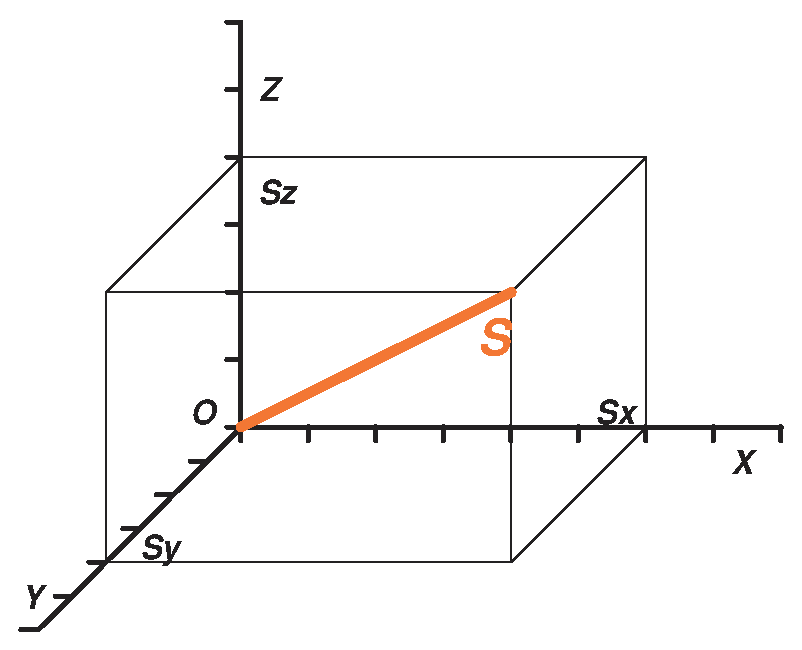
\includegraphics{GP002/GP002F01.eps}}
 \put( 170, 96){\makebox(0,0)[tr]{\parbox{85mm}
     {
     \begin{flushright}
      Пройденный путь: $S=f(t)$\\
      $S_x=f_1(t)$\\
      $S_y=f_2(t)$\\
      $S_z=f_3(t)$
     \end{flushright}
         }}}
  \end{picture}\\[3mm]
  \caption{\sf\Large Движение вдоль прямой.}
   \label{fig:straight_move}
\end{figure}  
%\newpage

{\bf\underline{Скорость равномерного движения} - физ. величина,
прямо пропорциональная пройденному пути
и обратно пропорцио\-нальная затраченному времени.}

\begin{displaymath}
v = \frac{\Delta S}{\Delta t}\;\;\;{\color{blue}(= const)}
\end{displaymath}
 \\[1mm]

{\bf\underline{\color{red}Неавномерное движение:}}

Пример на Рис.~\ref{fig:uneven_move}.

\begin{enumerate}
\item {\underline{\bf OA}} -- торможение
\item {\underline{\bf AB}} -- остановка (состояние покоя)
\item {\underline{\bf BC}} -- ускорение
\item {\underline{\bf CD}} -- равномерное движение
\end{enumerate}

 \begin{figure}[ht]
 \setlength{\unitlength}{1mm}
  \begin{picture}(180,100)(0,0)
  %\put(0,0){\framebox(180,110)[b]{}}
   \put(20,-3){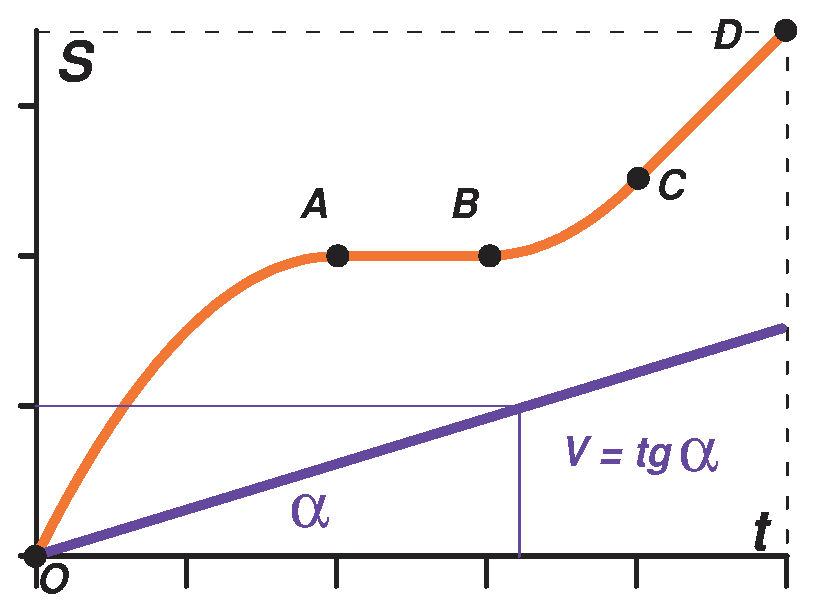
\includegraphics{GP002/GP002F02.eps}}
  \end{picture}\\[3mm]
  \caption{\sf\Large Неравномерное движение.}
   \label{fig:uneven_move}
\end{figure}

{\bf\underline{Средняя скорость:}}\hspace{10mm}
%\begin{displaymath}
$   v_{mean} =  \langle v\rangle  = \overline{v} =  \frac St$\\
%\end{displaymath}

{\bf\underline{Мгновенная скорость в момент $t=\tau$ :}}

\begin{displaymath}
   v(\tau) = \lim_{\Delta t\rightarrow0}\frac{S(\tau+\Delta t)-S(\tau)}{\Delta t} = \frac{dS}{dt}(\tau)= \dot{S}(\tau)
\end{displaymath}
%\newpage

 Путь, пройденный за время от $t_1$ до $t_2$ -- (Рис.~\ref{fig:aver_v_int})?
\begin{displaymath}
S = \sum_i \overline{v_i}\cdot \Delta t_i = \int_{t_1}^{t_2}v(t)dt
\end{displaymath}
 \\[1mm]

\begin{figure}[ht]
 \setlength{\unitlength}{1mm}
  \begin{picture}(180,110)(0,0)
  %\put(0,0){\framebox(180,110)[b]{}}
   \put(0,-3){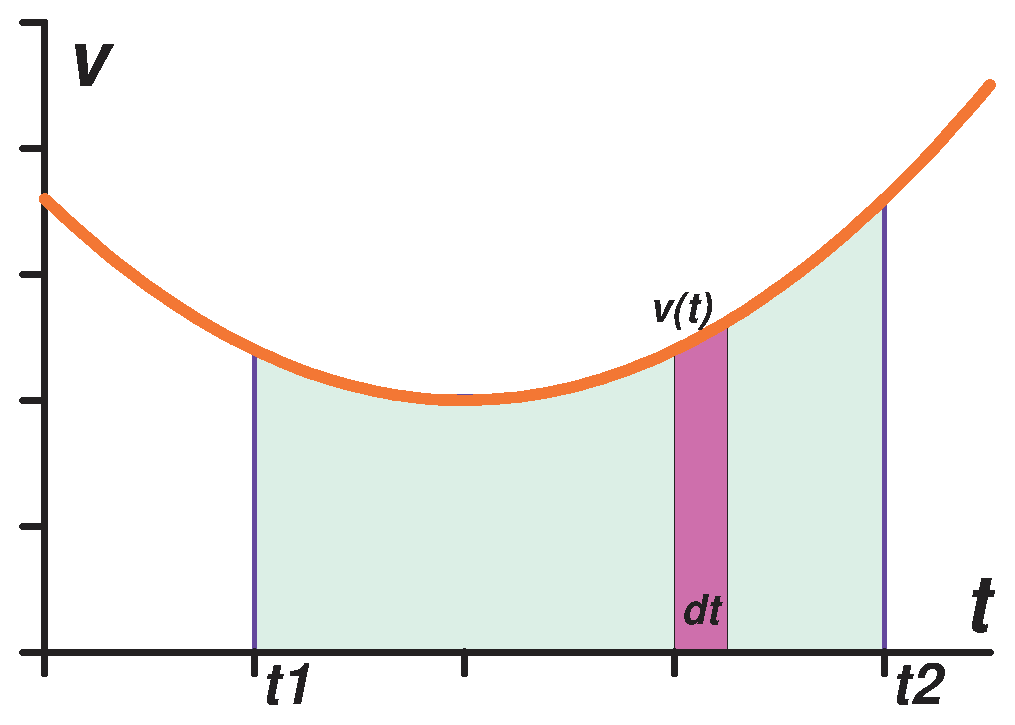
\includegraphics{GP002/GP002F03.eps}}
  \end{picture}\\[3mm]
\caption{\sf\Large Интегрирование для расчета средней скорости.}
   \label{fig:aver_v_int}
\end{figure}

\underline{\bf Равнопеременное прямолинейное движение}\\[2mm]

Ускорение (положительное или отрицательное):
\begin{displaymath}
v = v_0 + a\cdot t\;\;\;\;\;\;\;\;\;\;\;a = \frac{\Delta v}{\Delta t}
\end{displaymath}

Более точно:
\begin{displaymath}
a = \lim_{\Delta t\rightarrow 0}\left(\frac{\Delta v}{\Delta t}\right)=\frac{dv}{dt}=\dot{v}=\ddot{s}= const
\end{displaymath}

Путь:
\begin{displaymath}
S = \int_{t_1}^{t_2}v(t)dt = v_0\cdot (t_2-t_1) + \frac{a\cdot \left(t_2-t_1\right)^2}2
\end{displaymath}
%\newpage
\underline{\bf Произвольное прямолинейное движение}\\[2mm]

Если задан закон, по которому происходит движение
\begin{displaymath}
 S= f(t)\;\;\;,
\end{displaymath}

то мы всегда сможем найти скорость, ускорение и путь:
\begin{displaymath}
v = \dot{s} = \frac{df}{dt}
\end{displaymath}
\begin{displaymath}
a = \dot{v} = \ddot{s} = \frac{d^2f}{dt^2}
\end{displaymath}
\begin{displaymath}
s = s_2 - s_1 = f(t_2) - f(t_1) \rule[-7mm]{0mm}{12mm}
\end{displaymath}

Поскольку движение имеет {\bf направление}, то s, v и a -- векторы (обозначаются как {\bf s}, {\bf v}, {\bf a} или $\vec{s}$, $\vec{v}$, $\vec{a}$). Все сказанное справедливо (в векторном виде) для криволинейного движения. Положение в пространстве -- радиус-вектор $\vec{r}$ (Рис.~\ref{fig:vec_move}).\\

\begin{figure}[ht]
 \setlength{\unitlength}{1mm}
  \begin{picture}(180,110)(0,0)
  %\put(0,0){\framebox(180,110)[b]{}}
   \put(15,-3){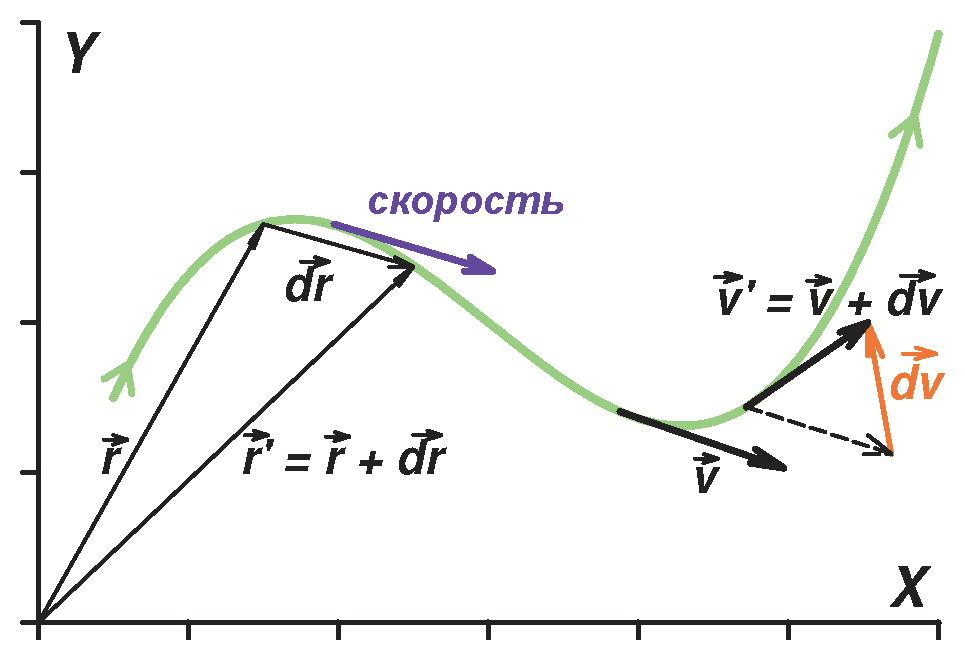
\includegraphics{GP002/GP002F04.eps}}
  \end{picture}\\[3mm]
  \caption{\sf\Large Векторная интерпретация движения.}
   \label{fig:vec_move}
\end{figure}

Составляющие ускорения -- тангенциальное и нормальное (радиальное, центростремительное, Рис.~\ref{fig:a_move}):
 $ \;\;\;\;\vec{a}\;=\;\vec{a_t}\;+\;\vec{a_n}$

\begin{figure}[ht]
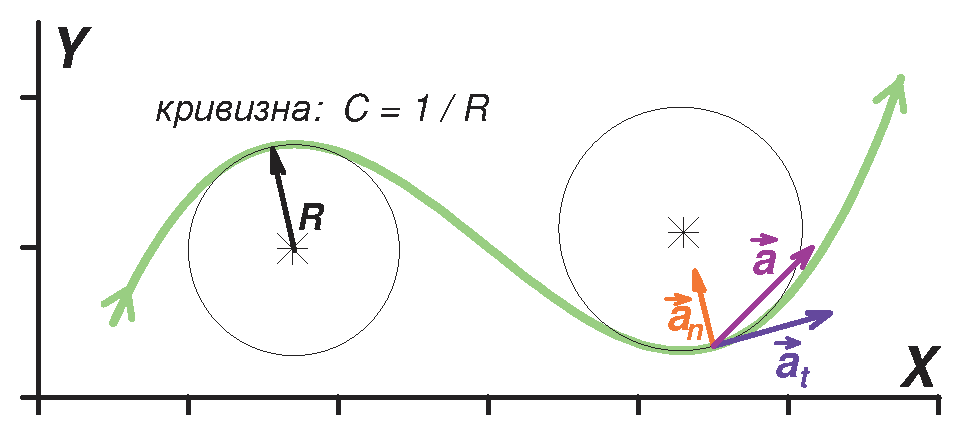
\includegraphics[width=0.8\textwidth]{GP002/GP002F05.eps}
% \setlength{\unitlength}{1mm}
%  \begin{picture}(180,45)(0,0)
%  %\put(0,0){\framebox(180,65)[b]{}}
%   \put(15,-3){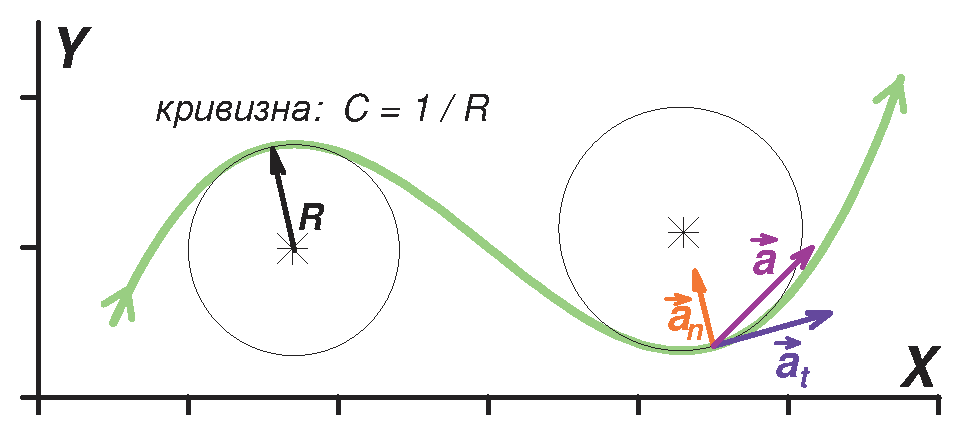
\includegraphics{GP002/GP002F05.eps}}
%  \end{picture}\\[1mm]
  \caption{\sf\Large Ускорение при движении.}
   \label{fig:a_move}
\end{figure}

Расчеты ускорения через пределы скоростей передвижения расчитываются (Рис.~\ref{fig:a_from_v_move}).

\begin{figure}[ht]
 \setlength{\unitlength}{1mm}
  \begin{picture}(180,80)(0,0)
  %\put(0,0){\framebox(180,70)[b]{}}
   \put(15,-3){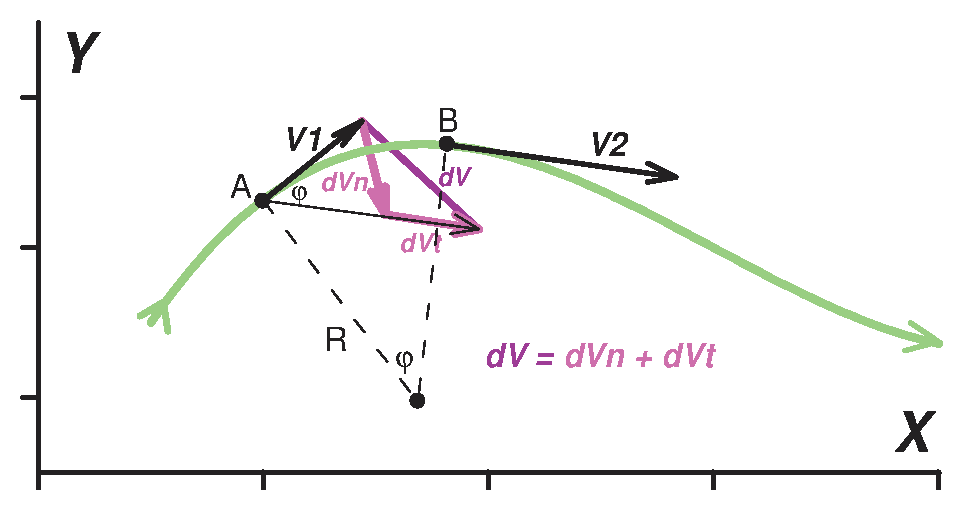
\includegraphics{GP002/GP002F06.eps}}
  \end{picture}\\[1mm]
  \caption{\sf\Large Расчет ускорения через пределы векторов скорости.}
   \label{fig:a_from_v_move}
\end{figure}

 \begin{displaymath}
  |dV_t| = |V_2|-|V_1|\;;\;\;\;\;\;  |dV_n| = |V_1|\cdot \varphi
 \end{displaymath}

 \begin{displaymath}
  |a_t| = \lim_{dt\rightarrow0}\frac{|dV_t|}{dt};\;\;\;\;\; \vec{a_t}\parallel\vec{V}
 \end{displaymath}

 \begin{displaymath}
  |a_n| = \lim_{dt\rightarrow0}\frac{|dV_n|}{dt} = \lim_{dt\rightarrow0}\frac{|V_1|\cdot\varphi}{dt}=
  \lim_{dt\rightarrow0}\left(|V_1|\cdot\frac{\varphi}{AB}\cdot\frac{AB}{dt}\right)=
  \frac{|V|^2}R
 \end{displaymath}

 \begin{displaymath}
  \vec{a_n}\parallel \vec{R}\perp \vec{V}
 \end{displaymath}

  \underline{Равномерное} движение по кривой: $\;\;\;|V|$=const, $\;\;\;\; \vec{a}=\vec{a_n}\perp\vec{V}$.

%\newpage
  \underline{\bf Кинематика (абсолютно) твердого тела}\\

  {\bf Поступательное движение --} все точки тела имеют одинаковые скорости и ускорения (Рис.~\ref{fig:trans_move}):

\begin{figure}[ht]
 \setlength{\unitlength}{1mm}
  \begin{picture}(150,60)(0,0)
  %\put(0,0){\framebox(180,80)[b]{}}
   \put(15,0){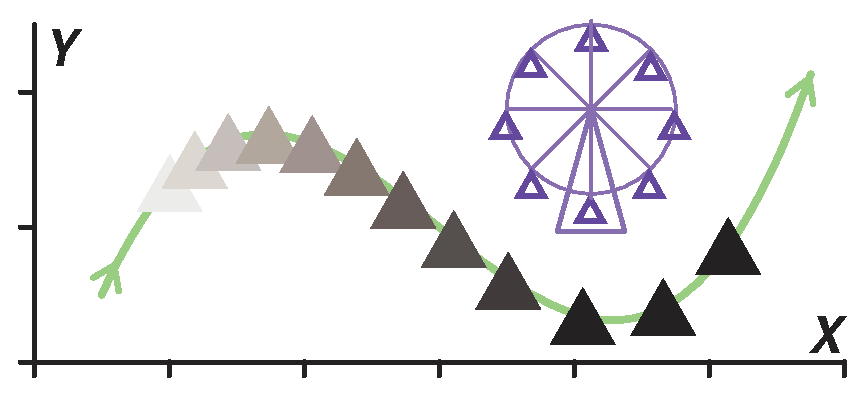
\includegraphics{GP002/GP002F07.eps}}
  \end{picture}\\[1mm]
  \caption{\sf\Large Поступательное движение твердого тела.}
   \label{fig:trans_move}
\end{figure}

\begin{figure}[ht]
 \setlength{\unitlength}{1mm}
  \begin{picture}(180,92)(0,0)
  %\put(0,0){\framebox(180,100)[b]{}}
   \put(0,0){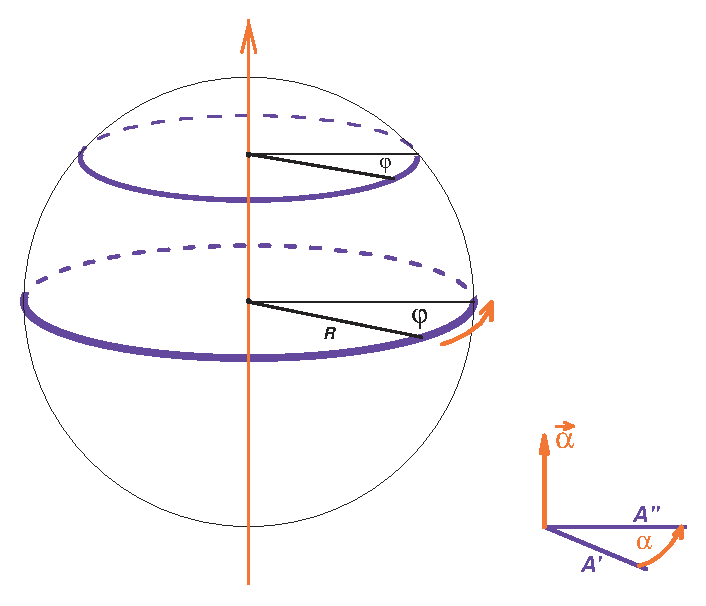
\includegraphics{GP002/GP002F08.eps}}
 \put( 180, 92){\makebox(0,0)[tr]{\parbox{85mm}
     {
     \centerline{\underline{Угловая скорость:}}
      \begin{displaymath}
      \omega=\dot{\varphi}=\frac{d\varphi}{dt}
      \end{displaymath}
     \centerline{\underline{Угловое ускорение:}}
      \begin{displaymath}
      \beta=\dot{\omega}=\ddot{\varphi}=\frac{d\omega}{dt}=\frac{d^2\varphi}{dt^2}
      \end{displaymath}
     }}}
 \put( 175, 0){\makebox(0,0)[br]{\parbox{50mm}
     {
      \centerline{Угол как вектор:}
      \begin{displaymath}
      \vec{\alpha}=\alpha\cdot\frac
          {\left[\vec{A'}\times\vec{A''}\right]}
          {\left|\left[\vec{A'}\times\vec{A''}\right]\right|}
      \end{displaymath}
     }}}
  \end{picture}\\
  \caption{\sf\Large Вращательное движение.}
   \label{fig:rot_move}
\end{figure}

  {\bf Вращение --} все точки тела описывают окружности с центрами на {\sl оси вращения} (Рис.~\ref{fig:rot_move}):

Связь линейной и угловой скорости:

      \begin{displaymath}
      V=\lim_{\Delta t\rightarrow0}\frac{\Delta S}{\Delta t}=\frac{d(R\cdot\varphi)}{dt}=
      \omega R;\;\;\;\;\;\;\;\vec{V}=\left[\vec{\omega}\times\vec{R}\right]
      \end{displaymath}
%\newpage

\underline{\bf Линейные и аксиальные векторы}\\

Линейные (истинные) векторы -- те, что связаны с поступательным движением или направлением в пространстве:

 \begin{displaymath}
 \vec{X}, \vec{Y}, \vec{Z}, \vec{V}, \vec{R}, \vec{a}, \vec{F},
 \end{displaymath}

Аксиальные векторы -- те, что связаны с вращением:

 \begin{displaymath}
 \vec{\varphi}, \vec{\alpha}, \vec{\beta}, \vec{L}, \vec{M}
 \end{displaymath}

Они отличаются своими свойствами симметрии: при зеркальном отра\-жении (то есть, при замене $X \rightarrow -X$) линейные векторы меняют знак, а аксиальные - не меняют (Рис.~\ref{fig:lin_axial_vecs}).

\begin{figure}[htp]
 \setlength{\unitlength}{1mm}
  \begin{picture}(180,150)(0,0)
  %\put(0,0){\framebox(180,150)[b]{}}
   \put(15,0){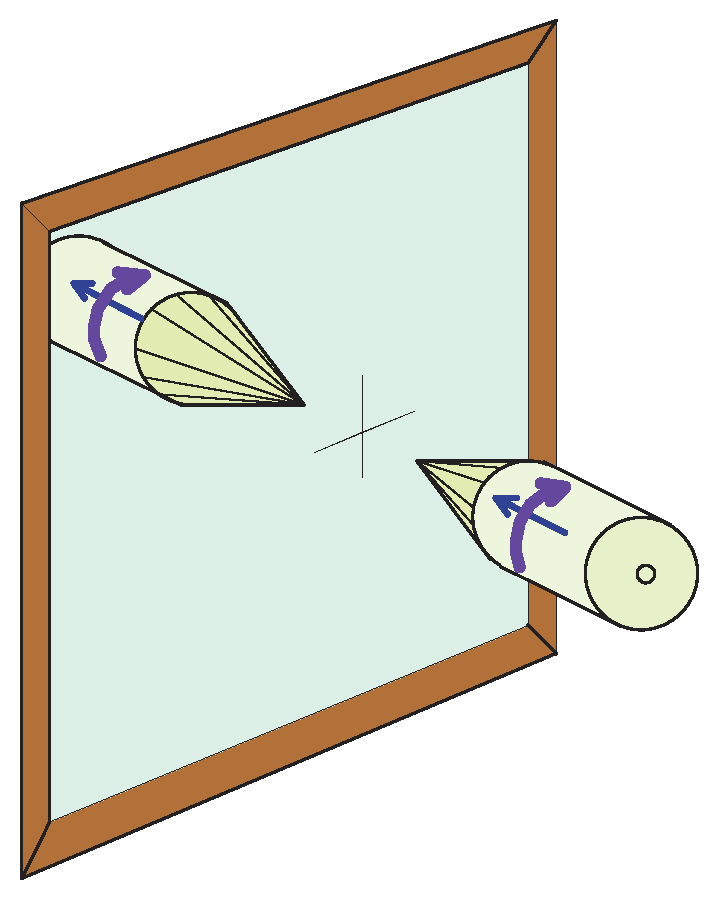
\includegraphics{GP002/GP002F09.eps}}
   \put(48, 105){\makebox(0,0)[c]{\color{blue}\Huge\bf $\vec{\omega}_2$}}
   \put(48, 70){\makebox(0,0)[c]{\color{red}\Huge\bf $\vec{V}_2$}}
   \put(120, 70){\makebox(0,0)[c]{\color{blue}\Huge\bf $\vec{\omega}_1$}}
   \put(120, 35){\makebox(0,0)[c]{\color{red}\Huge\bf $\vec{V}_1$}}
   \put(150,110){\makebox(0,0)[c]{\color{red}\Huge\bf $\vec{V}_2 = -\vec{V}_1$}}
   \put(150, 90){\makebox(0,0)[c]{\color{blue}\Huge\bf $\vec{\omega}_2 = +\vec{\omega}_1$}}
  \end{picture}\\[1mm]
  \caption{\sf\Large Отзеркаливание линейных и аксиальных векторов.}
   \label{fig:lin_axial_vecs}
\end{figure}
  
\newpage
\begin{flushright}
{\color{green}\LARGE\sl ШПАРГАЛКА}
\end{flushright}

\underline{\bf Связь декартовых и сферических координат}

Показана на Рис.~\ref{fig:dec_vs_sphe}.

 \begin{displaymath}
 \left\{\vec{x}, \vec{y}, \vec{z}\right\}
 \;\;\;\leftrightarrow \;\;\;
 \left\{\vec{r}, \vec{\theta}, \vec{\varphi}\right\}
 \end{displaymath}

\begin{figure}[ht]
 \setlength{\unitlength}{1mm}
  \begin{picture}(160,120)(0,0)
  %\put(0,0){\framebox(180,130)[b]{}}
   \put(25,0){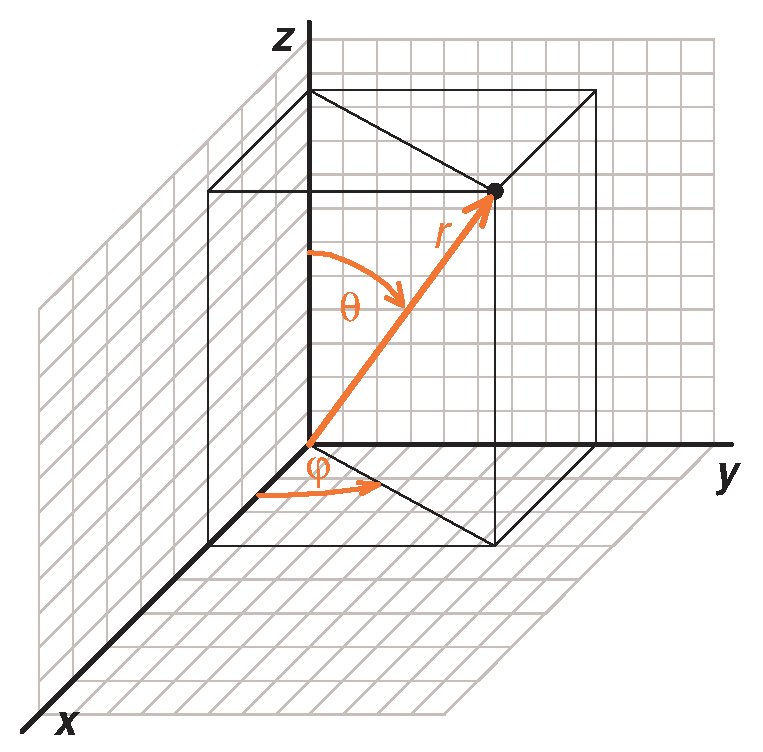
\includegraphics{GP002/GP002F10.eps}}
  \end{picture}\\[1mm]
  \caption{\sf\Large Связь декартовых и сферических координат.}
   \label{fig:dec_vs_sphe}
\end{figure}
 
 \begin{displaymath}
 \begin{array}{ccccc}
 0&\leq&r&&\\
 0&\leq&\theta&\leq&\pi\\
 0&\leq&\varphi&\leq&2\pi
 \end{array}
 \end{displaymath}

 \begin{displaymath}
 \left\{
 \begin{array}{ccl}
 x&=&r\sin\theta\cos\varphi\\
 y&=&r\sin\theta\sin\varphi\\
 z&=&r\cos\theta
 \end{array}
 \right\}\;\;\;
 \leftrightarrow\;\;\;
 \left\{
 \begin{array}{ccl}
 r&=&\sqrt{x^2+y^2+z^2}\\
 \theta&=&\arccos\left(z/r\right)\\
 \varphi&=&\arctan\left(y/x\right)
 \end{array}
 \right\}
 \end{displaymath}

 \begin{displaymath}
dx\cdot dy\cdot dz\;\;=\;\;dV\;\;=\;\;r^2\cdot dr\cdot\sin\theta\cdot d\theta\cdot d\varphi
 \end{displaymath}

%\newpage
\begin{flushright}
{\color{green}\LARGE\sl ШПАРГАЛКА}
\end{flushright}
\centerline{\huge\underline{Правила векторной алгебры}}
\begin{itemize}
\item длина вектора (модуль):
 \begin{displaymath}
 |\vec{A}| = \sqrt{A_x^2+A_y^2+A_z^2}
 \end{displaymath}
\item сложение (вычитание):
 \begin{displaymath}
 \vec{C} = \vec{A} \pm \vec{B}\;\;\;\Leftrightarrow\;\;\;
 \left\{\begin{array}{cc}C_x &= A_x\pm B_x\\
                         C_y &= A_y\pm B_y\\
                         C_z &= A_z\pm B_z\end{array}\right.
 \end{displaymath}
\item умножение на число (масштабирование):
 \begin{displaymath}
 \vec{C} = k\cdot\vec{A} \;\;\;\Leftrightarrow\;\;\;
 \left\{\begin{array}{cc}C_x &= k\cdot A_x\\
                         C_y &= k\cdot A_y\\
                         C_z &= k\cdot A_z\end{array}\right.
 \end{displaymath}
\item дифференцирование:
 \begin{displaymath}
 \vec{C} = \frac{\vec{dA}}{dt} \;\;\;\Leftrightarrow\;\;\;
 \left\{\begin{array}{cc}C_x &= {dA_x}/{dt}\\
                         C_y &= {dA_y}/{dt}\\
                         C_z &= {dA_z}/{dt}\end{array}\right.
 \end{displaymath}
\item скалярное перемножение двух векторов:
 \begin{displaymath}
 C = \left(\vec{A},\vec{B}\right) = \vec{A}\cdot\vec{B}\;\;\;\Leftrightarrow\;\;\;
 C = A_x\cdot B_x + A_y\cdot B_y + A_z\cdot B_z =|A|\cdot|B|\cdot \cos\theta
\end{displaymath}
\item векторное перемножение двух векторов:
 \begin{displaymath}
 \vec{C} = \left[\vec{A},\vec{B}\right] = \vec{A}\times\vec{B}\;\;\;\Leftrightarrow\;\;\;
 \left\{\begin{array}{cc}C_x &= A_y\cdot B_z - A_z\cdot B_y\\
                         C_y &= A_z\cdot B_x - A_x\cdot B_z\\
                         C_z &= A_x\cdot B_y - A_y\cdot B_z\end{array}\right.
 \end{displaymath}
 \begin{displaymath}
  |C|=|A|\cdot|B|\cdot\sin\theta;\;\;\;\; \vec{C}\perp\vec{A};\;\;\;\vec{C}\perp\vec{B}
\end{displaymath}
\end{itemize}



\chapter{Динамика}
\sf\Large

%\section{Динамика}
%\centerline{\underline{\Huge\bf ДИНАМИКА}}

\centerline{\sl Изучает взаимодействие тел, приводящее к изменению их движения}
\vspace{2mm}
\section{Первый закон Ньютона (принцип инерции)}
%\underline{\bf Первый закон Ньютона (принцип инерции)}

\begin{center}
\fbox{\parbox{180mm}{\color{blue}\bf Всякое тело сохраняет состояние покоя или равномерного и прямолинейного движения, пока
воздействие со стороны других тел не заставит его изменить это состояние.}}\\[1mm]
(Здесь тело -- как материальная точка, то есть, вращение исключается.)
\end{center}

Наблюдения: 1зН справедлив не для каждой системы отсчета.

\fbox{Инерциальная система} -- та, по отношению к которой 1зН выполняется.

Гелиоцентрическая система. Всякая система, движущаяся относительно нее равномерно и прямолинейно.
\fbox{\color{blue}Инерциальные системы существуют.}\\

\section{Второй закон Ньютона}

%\underline{\bf Второй закон Ньютона}

\begin{center}
\fbox{\parbox{180mm}{\color{blue}\bf Изменение движения пропорционально приложенной силе и происходит в том направлении, в каком действует сила.}}\\[1mm]
\end{center}
Физ. величина СИЛА характеризует воздействие одних тел на другие, в результате которого тела приобретают ускорение.
\begin{displaymath}
 f=k\cdot a\;\;\;\;\;\;\;\;\vec{f}=k\cdot\vec{a}
 \end{displaymath}
Более удобное измерение силы: пружинный динамометр (Рис.~\ref{fig:force_dina}).\\
 
 \begin{figure}[ht]
 \setlength{\unitlength}{1mm}
  \begin{picture}(180,40)(0,0)
   %\put(0,0){\framebox(180,40)[b]{}}
   \put(15,0){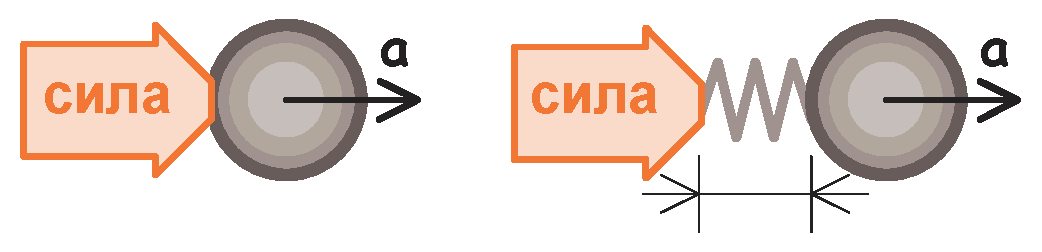
\includegraphics{GP003/GP003F01.eps}}
  \end{picture}\\[1mm]
    \caption{Сила и ее измерение пружинным динамометром.}
   \label{fig:force_dina}
\end{figure}
  
Опыт: {\bf разные} тела от {\bf одинаковой} силы получают {\bf разные} ускорения. Это свойство тел -- физ. величина ИНЕРЦИОННАЯ МАССА.\\
Ньютон: МАССА - это мера количества материи в теле {\sl (не совсем верно)}. МАССА - это именно мера инерции.\\
М.В.Ломоносов: масса изолированной системы = const.
\begin{displaymath}
 \vec{a}=k\cdot\vec{f}/m
 \end{displaymath}
%\newpage
Упругие силы, силы тяготения. \underline{\bf Силы трения} -- молекулярное взаимо\-действие между соприкасающимися телами. Трение внешнее (между телом и другими телами; трение покоя) и внутреннее (движение жидкостей и газов).

Сила трения всегда направлена противоположно скорости (Рис.~\ref{fig:fric_force}). Чтобы тело двигалось без ускорения, надо, чтобы внешняя сила уравновешивала силу трения.

\begin{figure}[ht]
 \setlength{\unitlength}{1mm}
  \begin{picture}(180,35)(0,0)
   %\put(0,0){\framebox(180,40)[b]{}}
   \put(10,0){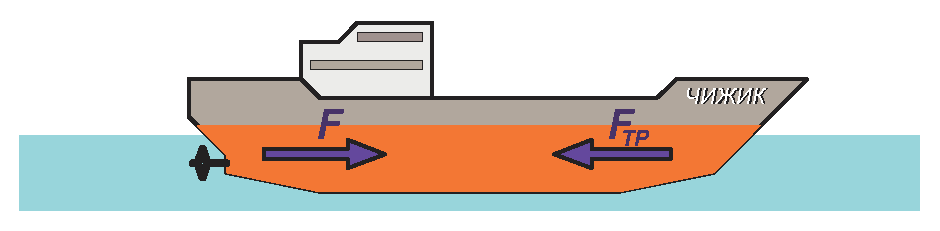
\includegraphics{GP003/GP003F02.eps}}
  \end{picture}\\[1mm]
  \caption{Сила трения всегда направлена против движения.}
   \label{fig:fric_force}
\end{figure}

Парашютист: 60 м/с (открытие парашюта) => 5-6 м/с.

Сила трения скольжения приблизительно пропорциональна сжи\-мающей силе $F_n$ (Рис.~\ref{fig:fric_vec_force}):
\begin{displaymath}
 F_{TP}\simeq\chi\cdot F_n
 \end{displaymath}

\begin{figure}[ht]
 \setlength{\unitlength}{1mm}
  \begin{picture}(180,55)(0,0)
   %\put(0,0){\framebox(180,40)[b]{}}
   \put(45,0){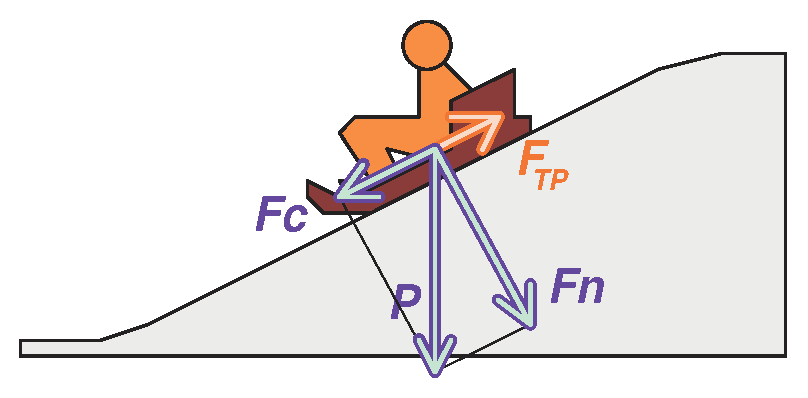
\includegraphics{GP003/GP003F03.eps}}
   \put(0,50){\makebox(0,0)[tl]{\parbox{60mm}{коэффициент трения $\chi$ зависит от состояния поверхностей и от скорости скольжения}}}
  \end{picture}\\[1mm]
\caption{Векторизация силы трения.}
   \label{fig:fric_vec_force}
\end{figure}

Динамика силы трения при начале движения (Рис.~\ref{fig:fric_dyn}).

\begin{figure}[ht]
 \setlength{\unitlength}{1mm}
  \begin{picture}(180,55)(0,0)
   %\put(0,0){\framebox(180,40)[b]{}}
   \put(5,0){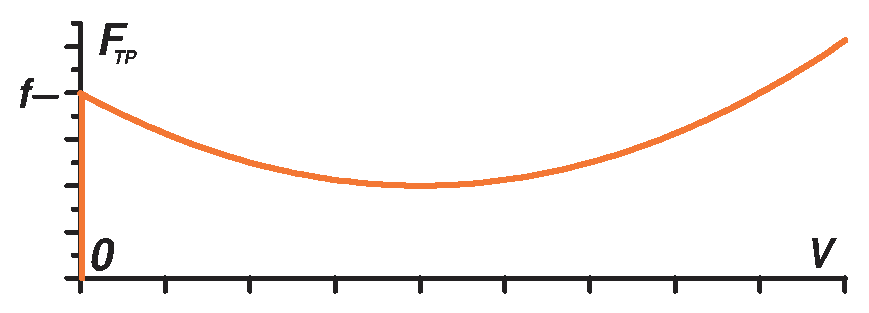
\includegraphics{GP003/GP003F04.eps}}
   \put(80,40){\makebox(0,0)[c]{\parbox{85mm}{При V=0 сила трения может быть от 0 до некоего максимума $f$, а при начале движения снижается}}}
   \put(178,30){\makebox(0,0)[tr]{\bf авто: ABS}}
  \end{picture}
    \caption{Динамика силы трения при начале движения.}
   \label{fig:fric_dyn}
\end{figure}

%\newpage
Рассмотрим движение под действием постоянной силы $\vec{f}$ за время $\Delta t$. Используя 2зН, получим:
\begin{displaymath}
  k\cdot\frac{\vec{f}}{m}=\vec{a}=\frac{\vec{v_2}-\vec{v_1}}{\Delta t}
\end{displaymath}
или, домножив на $m$ и $\Delta t$ :
\begin{displaymath}
 m\vec{v_2}-m\vec{v_1} = k\cdot\vec{f}  \Delta t
\end{displaymath}
Величина $m\vec{v}$ имеет большой физический смысл и называется КОЛИЧЕСТ\-ВО ДВИЖЕНИЯ или ИМПУЛЬС (обозначается как $\vec{p}$ -- от англ. {\sl pulse}).
\begin{displaymath}
\vec{p}\equiv m\vec{v}\hspace{40mm} \frac{\vec{dp}}{dt} = k\cdot\vec{f}
\end{displaymath}

Еще одно определение СИЛЫ: Сила -- векторная величина, пропорцио\-нальная вызываемому ею изменению импульса в единицу времени.

Величина $\vec{f}\Delta t$ тоже имеет персональное название -- ИМПУЛЬС СИЛЫ.

Если положить коэф-т $k$ равным 1, то можно установить единицы измерения для $f$.
\begin{itemize}
\item CGS: $[m]$= г, $\;\;[a]$= см/с$^2\;\;\;\;\Rightarrow\;\;\;[f]$= дина = г$\cdot$см/с$^2$
\item SI: $\;\;\;[m]$= кг, $\;[a]$= м/с$^2\;\;\;\;\Rightarrow\;\;\;[f]$= Ньютон = кг$\cdot$м/с$^2 = 10^5$дин
\end{itemize}
\vspace{2mm}

\underline{\bf Механический принцип относительности (Галилей)}

1зН -- частный случай 2зН при $f=0$.

Движение тела относительно двух различных ниерциальных систем отличается лишь на постоянную разность скоростей, а ускорения -- одина\-ковы. $\Rightarrow$ и силы (по 2зН) одинаковы!\\[3mm]
\fbox{\parbox{185mm}{\color{blue}\bf Никакими механическими опытами, производимыми внутри системы, нельзя решить -- находится ли инерциальная система в состоянии покоя или она равномерно и прямолинейно движется. \color{black}\sl Галилей, 1632 г.  }}\\[1mm]

Принцип относительности Эйнштейна: ({\color{blue}механическими})$\rightarrow$({\color{red}любыми: меха\-ническими, электрическими, оптическими, etc.})
%\newpage

\section{Третий закон Ньютона}

%\underline{\bf Третий закон Ньютона} {(\sl Как аукнется -- так и откликнется)}

{\sl Как аукнется -- так и откликнется!}

\begin{center}
\fbox{\parbox{180mm}{\color{blue}\bf Если тело {\bf B} воздействует на тело {\bf A} с силой $\vec{f_1}$, то и тело {\bf A}, в свою очередь, воздействует на тело {\bf B} с силой $\vec{f_2}$, причем $\vec{f_1}=-\vec{f_2}$.} (Рис.~\ref{fig:new_3law})}
\end{center}
%\\[1mm]

\begin{figure}[ht]
 \setlength{\unitlength}{1mm}
  \begin{picture}(180,65)(0,0)
   %\put(0,0){\framebox(180,65)[b]{}}
   \put(0,0){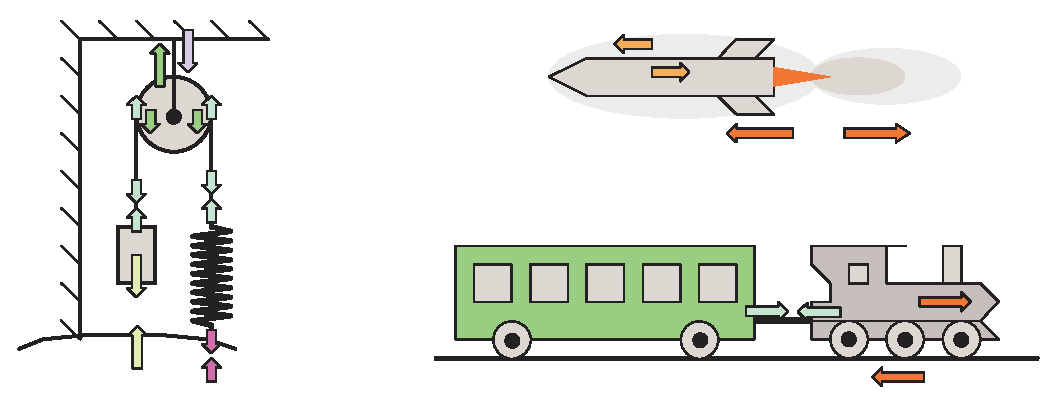
\includegraphics{GP003/GP003F05.eps}}
  \end{picture}\\[1mm]
  \caption{Баланс действия и противодействия (третий закон Ньютона).}
   \label{fig:new_3law}
\end{figure}

Итак, если взаимодействуют 2 тела A и B ;) с массами $m_1$ и $m_2$, то оба приобретают противоположные ускорения:
\begin{displaymath}
\vec{a_1}=\frac{f_1}{m_1},\;\;\;\;\;\;\vec{a_2}=\frac{f_2}{m_2}
\end{displaymath}

Из 3зН следует, что $\vec{f_1}=-\vec{f_2}$, и поэтому
\begin{displaymath}
\vec{a_1}=-\frac{m_2}{m_1}\cdot\vec{a_2}
\end{displaymath}

Изменение количества движения тел A и B:
\begin{displaymath}
\vec{\Delta p_1}=\vec{f_1}\cdot\Delta t\;\;\;\;\;\;\;\vec{\Delta p_2}=
\vec{f_2}\cdot\Delta t=-\vec{\Delta p_1}
\end{displaymath}

\begin{center}
\fbox{\parbox{180mm}{\color{blue}\bf Насколько в результате взаимодействия импульс одного тела увеличился, настолько импульс другого тела уменьшился.}}\\[1mm]
\end{center}

Обобщая на всю систему из N тел, получаем ЗАКОН СОХРАНЕ\-НИЯ КОЛИЧЕСТВА ДВИЖЕНИЯ (ИМПУЛЬСА): $\sum\vec{p} = $const.

\begin{center}
\fbox{\parbox{180mm}{\color{blue}\bf Полный импульс замкнутой системы остается постоянным во все время движения. \color{red}\sl (Не обнаружено нарушений ни в микро-, ни в макро-мире, ни в квантовой, ни в релятивистской механике)}}
\end{center}

%\newpage
Поскольку импульс --- это вектор, то закон сохранения выполняется отдельно для каждой его составляющей (Рис.~\ref{fig:comp_imp_save}):

\begin{figure}[ht]
 \setlength{\unitlength}{1mm}
  \begin{picture}(180,50)(0,0)
   %\put(0,0){\framebox(180,65)[b]{}}
   \put(0,0){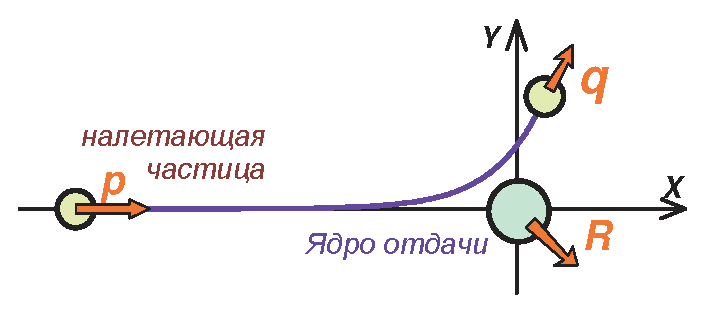
\includegraphics{GP003/GP003F06.eps}}
   \put(180,40){\makebox(0,0)[rt]{\parbox{60mm}{\begin{displaymath}
                                            \left\{ \begin{array}{ccc}
                                            p_x&=&R_x+q_x\\
                                            0&=&R_y+q_y\\
                                            0&=&R_z+q_z
                                                    \end{array}
                                            \right.
                                               \end{displaymath}}}}
  \end{picture}\\[1mm]
  \caption{Сохранение компонент импульса.}
   \label{fig:comp_imp_save}
\end{figure}

\begin{figure}[h]
\centering
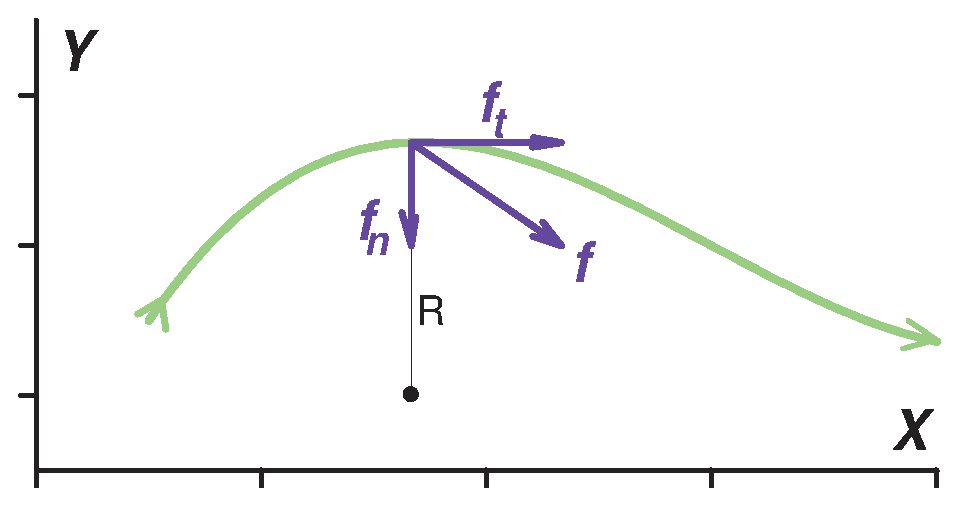
\includegraphics[width=0.8\textwidth]{GP003/GP003F07.eps}
% \setlength{\unitlength}{1mm}
%  \begin{picture}(180,80)(0,0)
%   %\put(0,0){\framebox(180,90)[b]{}}
%   \put(0,0){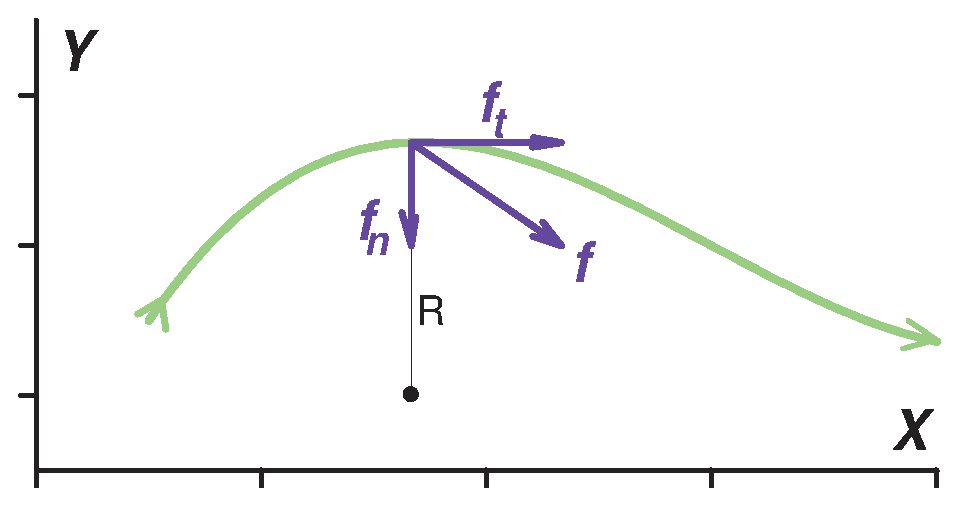
\includegraphics{GP003/GP003F07.eps}}
%  \end{picture}\\
  \caption{Векторный расклад сил при криволинейном движении.}
   \label{fig:vecurve}
\end{figure}

Для изолированной системы из N тел:

\begin{displaymath}
 \vec{P}=\sum_i^N\vec{p_i}=const\;\;\;\Leftrightarrow\;\;\;
 \left\{ \begin{array}{ccccc}
 P_x&=& \sum_{i=1}^N p_{xi}&=&const\\
 P_y&=& \sum_{i=1}^N p_{yi}&=&const\\
 P_z&=& \sum_{i=1}^N p_{zi}&=&const
 \end{array}
 \right.
\end{displaymath}
\hspace{3mm}

\underline{\bf Силы при криволинейном движении}

Как и ускорение, сила имеет 2 компонента (Рис.~\ref{fig:vecurve}):

\begin{enumerate}
\item тенгенциальная сила ($\vec{f_t}\parallel\vec{v}$ -- разгоняет или тормозит)
\item центростремительная сила ($\vec{f_n}\perp\vec{v}$ -- заставляет менять направление)
\end{enumerate}

\begin{displaymath} \vec{f}=\vec{f_t}+\vec{F_n};\;\;\;\;\;\;\;|f|=\sqrt{f_t^2+f_n^2};\;\;\;\;\;\;\;\;
 |f_n|=ma_n=m \frac{v^2}{R}
\end{displaymath}

%\newpage
\noindent
Равномерное движение по кривой: $f_t=0$. Вся сила -- центростремительная.\\[4mm]
Равномерное движение по окружности: $R=$const., $v=\omega R$
\begin{displaymath}
 f_n=m \frac{v^2}{R}=m\omega^2R=4\pi^2m\frac{R}{T^2}
\end{displaymath}

\underline{Центростремительная} сила приложена к телу, а равная ей (но противопо\-ложная по направлению) \underline{центробежная} -- к связям. В реальных задачах иногда требуется компенсация (Рис.~\ref{fig:vagon_balance}).
\\

\begin{figure}[ht]
 \setlength{\unitlength}{1mm}
  \begin{picture}(180,60)(0,0)
   %\put(0,0){\framebox(180,65)[b]{}}
   \put(85,0){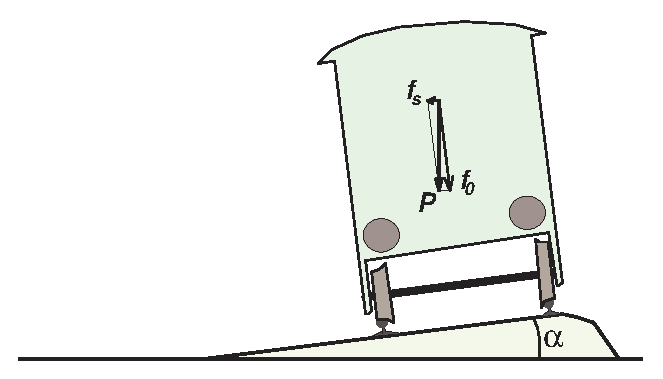
\includegraphics{GP003/GP003F08.eps}}
   \put(0,0){\makebox(0,0)[bl]{\parbox{130mm}{\sf\Large
    Неподвижный вагон, кроме нормальной к рельсам силы $f_0$, оказывает на них боковое давление с силой $f_s=P\;{\rm tg}\alpha$. Надо, чтобы при движении центробежная сила ее скомпенсировала:
   \begin{displaymath}
   P\cdot tg\alpha = mg\cdot tg\alpha = \frac{mv^2}{R}\;\;\;\;\Rightarrow\;\;\;
   tg\alpha = \frac{mv^2}{Rg}
   \end{displaymath}}}}
  \end{picture}\\[1mm]
  \caption{Наклон вагона для компенсации бокового давления при движении по окружности.}
   \label{fig:vagon_balance}
\end{figure}

\newpage
\underline{\bf Ускоренные системы}
\\

В ускоренных системах возникают силы, действующие на компоненты системы (Рис.~\ref{fig:a_system}). 

\begin{figure}[ht]
 \setlength{\unitlength}{1mm}
  \begin{picture}(180,40)(0,0)
   %\put(0,0){\framebox(180,65)[b]{}}
   \put(0,0){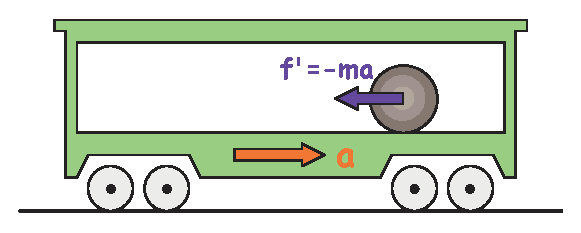
\includegraphics{GP003/GP003F09.eps}}
   \put(190,0){\makebox(0,0)[br]{\parbox{90mm}{\sf\Large
   В Лаб.системе: вагон ускоряется, шар отстает.\\
   В системе вагона: шар покатился назад с ускорением $-a$, как если бы появилась сила
   $\vec{f}=-m\vec{a}$
   }}}
  \end{picture}\\[1mm]
  \caption{Силы в ускоренной системе.}
   \label{fig:a_system}
\end{figure}

Фиктивная сила, которую приходится вводить в ускоренной системе отсчета, чтобы в ней выполнялся 2 закон Ньютона -- \underline{инерционная сила} или \underline{сила инерции} (Рис.~\ref{fig:iner_a_sys}).
\\

\begin{figure}[ht]
 \setlength{\unitlength}{1mm}
  \begin{picture}(180,90)(0,0)
   %\put(0,0){\framebox(180,80)[b]{}}
   \put(0,0){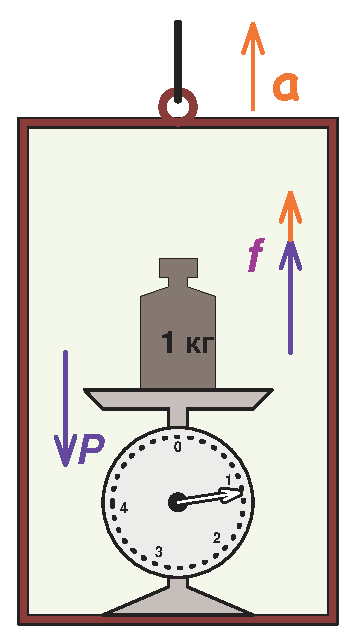
\includegraphics{GP003/GP003F10.eps}}
   \put(190,0){\makebox(0,0)[br]{\parbox{130mm}{\sf\large
   \begin{enumerate}
   \item{\bf $\vec{a}=0$ (Лифт стоит на месте или движется равномерно.)}
        Гиря давит на весы своим весом $\vec{P}=m\vec{g}$. Весы давят на гирю с такой же силой и уравновешивают ее вес. (В обеих {\bf инерциальных} системах координат)
   \item{\bf $\vec{a}>0$ (Лифт ускоряется вверх.)}
    \begin{itemize}
    \item В Лаб.системе: Чтобы гиря тоже начала ускоряться вместе с лифтом, весы давят на нее снизу с дополнительной силой $\vec{f\prime}=m\vec{a}$. По 3зН гиря давит на весы с такой же силой.
    \item В системе лифта: появилась сила инерции $\vec{f\prime\prime}=-m\vec{a}$, которая добавилась к весу гири.
    \end{itemize}
   \end{enumerate}
   }}}
  \end{picture}\\[1mm]
    \caption{Силы инерции в ускоренной системе.}
   \label{fig:iner_a_sys}
\end{figure}

  ОТО Эйнштейна: Вселенная относительно системы лифта дернулась вниз с ускорением $-\vec{a}$ и создала дополнительное гравитационное поле, направ\-ленное туда же:
   $g\;\;\;\rightarrow\;\;\;g\prime=(g+a)$.\\[1mm]

%\newpage
\underline{\bf Вращающиеся системы}

Баланс сил во вращающейся системе показан на Рис.~\ref{fig:rot_sys_balance}.

\begin{figure}[ht]
 \setlength{\unitlength}{1mm}
  \begin{picture}(180,100)(0,0)
   %\put(0,0){\framebox(180,65)[b]{}}
   \put(0,0){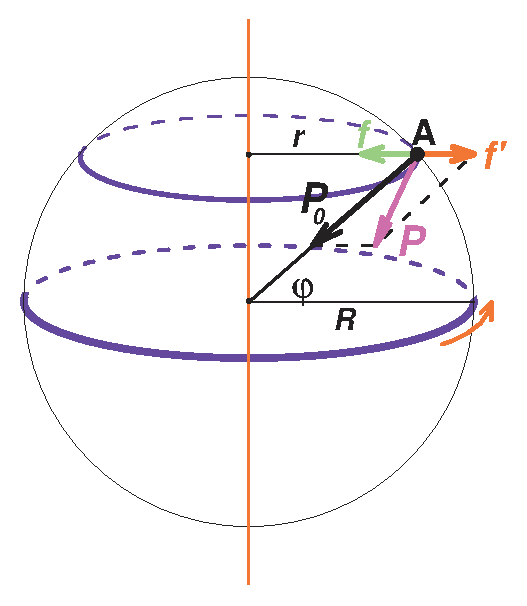
\includegraphics{GP003/GP003F11.eps}}
   \put(190,0){\makebox(0,0)[br]{\parbox{100mm}{\sf\Large
   В инерциальной гелиоцентрической системе: чтобы тело А на широте $\varphi$ вращалось вместе с Землей вокруг ее оси, надо, чтобы часть его веса $P_0$ играла роль центростремительной силы ${\color{green}f}=m\omega^2r=m\omega^2R\cos\varphi$.\\
   В системе, связанной с Землей: 1) направленный к центру Земли вес $P_0$  и 2) {\sl инерционная центробежная сила} ${\color{red}f\prime}=m\omega^2r$, направленная от оси. Их сумма - кажущийся вес ${\color{magenta}P}$.\\
   Масштаб: $f/P_0=\omega^2R\cos\varphi/g\simeq\cos\varphi/289$
   }}}
  \end{picture}\\[1mm]
  \caption{Баланс сил во вращающейся системе.}
   \label{fig:rot_sys_balance}
\end{figure}
  
На экваторе ($\varphi=0$): $f/P_0$ -- максимально; \hfill{} $f_{\max}/P_0=\omega^2R/g=v^2/gR$\\
Обращается в 1 при $v=\sqrt{gR}\simeq7.9$ км/с

\newpage

\centerline{\underline{\bf Сила Кориолиса}}

% \begin{figure}[ht]
 \setlength{\unitlength}{1mm}
  \begin{picture}(180,240)(0,0)
   %\put(-5,-10){\framebox(180,240)[b]{}}
   \put(0,-10){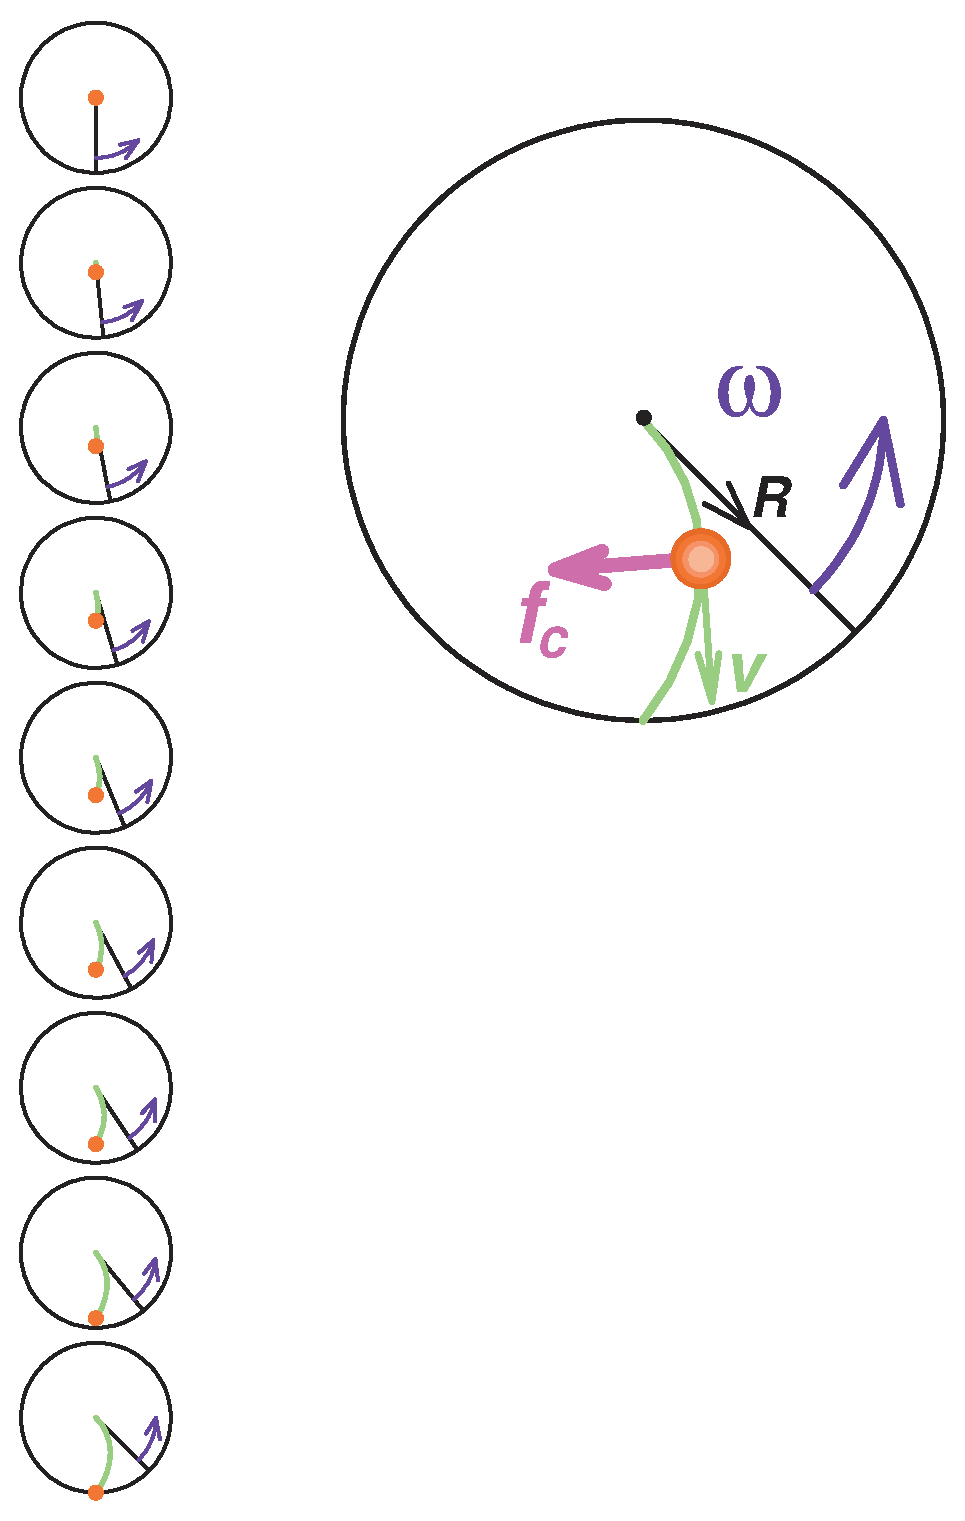
\includegraphics{GP003/GP003F12.eps}}
   \put(100,231){\makebox(0,0)[c]{Шарик катится по вращающемуся диску:}}
   \put(35,120){\makebox(0,0)[tl]{\parbox{40mm}{В лабораторной (инерциальной!) системе -- O.K. }}}
   \put(180,115){\makebox(0,0)[tr]{\parbox{80mm}{В системе диска шарик сносит вправо, как если бы на него действовала сила $\vec{f_c}\perp\vec{v}$}}}
   \put(180,0){\makebox(0,0)[br]{\parbox{150mm}{Мы живем в такой вращающейся системе. Чтобы корректно объяснить все явления, у нас $\exists$ два выхода:
   \begin{enumerate}
   \item Каждый раз переделывать все формулы, учитывая вращение системы координат
   \item Ввести фиктивную (как и силу инерции) Кориолисову силу $\vec{f_c}$, которая $\perp$ скорости $\vec{v}$ и оси вращения $\vec{\omega}$.
   \end{enumerate}
   \begin{displaymath}
    \vec{f_c}=2m\left[\vec{v}\times\vec{\omega}\right]
   \end{displaymath}
   }}}
  \end{picture}\\[1mm]
%  \caption{.}
%   \label{fig:}
%\end{figure}
  
\underline{\bf Вывод формулы для силы Кориолиса} \hfill{ } {\color{green}\sl (факультативно)}

Пусть тело движется со скоростью $\vec{v}$ и ускорением $\vec{a}$ в неинерциальной системе координат, которая вращается с угловой скоростью $\vec{\omega}$ и угловым ускорением $\vec{\beta}$. Если радиус вращения тела равен $\vec{R}$,
то линейная скорость $\vec{v\prime}$ во внешней \underline{инерциальной} системе равна:
   \begin{displaymath}
    \vec{v\prime}= \vec{v}+\left[\vec{\omega}\times\vec{R}\right]
   \end{displaymath}
 Ускорение $\vec{a\prime}$ этой инерциальной системе равно:
   \begin{displaymath}
   \vec{a\prime}= \frac{d}{dt}\left(\vec{v\prime}\right) =
   \frac{d}{dt}\left(\vec{v}\right) +
   \frac{d}{dt}\left[\vec{\omega}\times\vec{R}\right]=
   \frac{d}{dt}\left(\vec{v}\right) +
   \left[\frac{d}{dt}\left(\vec{\omega}\right)\times\vec{R}\right] +
   \left[\vec{\omega}\times\frac{d}{dt}\left(\vec{R}\right)\right]\;.
   \end{displaymath}
 Учитывая, что
   \begin{displaymath}
   \frac{d}{dt}\left(\vec{v}\right) = \vec{a}+\left[\vec{\omega}\times\vec{v}\right],
   \end{displaymath}
 а скорость изменения радиуса
   \begin{displaymath}
   \frac{d}{dt}\left(\vec{R}\right) = \vec{v}+\left[\vec{\omega}\times\vec{R}\right],
   \end{displaymath}
получим:
   \begin{displaymath}
   \vec{a\prime}=
   \vec{a}+
   \left[\vec{\omega}\times\vec{v}\right]+
   \left[\vec{\beta}\times\vec{R}\right]+
   \left[\vec{\omega}\times\vec{v}\right]+
   \left[\vec{\omega}\times\left[\vec{\omega}\times\vec{R}\right]\right].
      \end{displaymath}
Далее воспользуемся свойством тройного векторного произведения
   \begin{displaymath}
\left[\vec{A}\times\vec{B}\times\vec{C}\right] =
\vec{B}\cdot\left(\vec{A}\cdot\vec{C}\right) -
\vec{C}\cdot\left(\vec{A}\cdot\vec{B}\right),
      \end{displaymath}
а также тем фактом, что векторы $\vec{\omega}$ и $\vec{R}$ взаимно перпендикулярны, и потому их скалярное произведение равно нулю:
   \begin{displaymath}
   \left[\vec{\omega}\times\left[\vec{\omega}\times\vec{R}\right]\right]=
   \vec{\omega}\cdot\left(\vec{\omega}\cdot\vec{R}\right)-
   \vec{R}\cdot\left(\vec{\omega}\cdot\vec{\omega}\right)=
   -\vec{R}\cdot\omega^2.
   \end{displaymath}
Итак, получаем, что ускорение тела относительно инерциальной системы, в которой просто обязаны соблюдаться все законы Ньютона, равно:
   \begin{displaymath}
   \vec{a\prime}=
   \vec{a}+
   \left[\vec{\beta}\times\vec{R}\right]-
   2\left[\vec{v}\times\vec{\omega}\right]-
   \omega^2\vec{R}.
   \end{displaymath}
 Если почленно умножить все это на массу $m$, то в последнем слагаемом узнаем центростремительную силу, которая должна уравновесить силу инерции, направленную по радиусу, а в предпоследнем - силу, которая должна скомпенсировать силу Кориолиса (если мы не хотим, чтобы тело отклонилось от своего заданного движения в неинерциальной системе).



\chapter{Работа и энергия}
\sf\Large

%\centerline{\underline{\Huge\bf РАБОТА и ЭНЕРГИЯ}}
%\hspace{3mm}

Сила $\vec{f}$ вызывает перемещение тела. Характеристика ее действия -- это РАБОТА {\sl (\underline{A}ction)}.\\

Баланс сил при перемещении тела показан на Рис.~\ref{fig:body_move}

\begin{figure}[ht]
 \setlength{\unitlength}{1mm}
  \begin{picture}(190,50)(0,0)
   %\put(0,0){\framebox(190,40)[b]{}}
   \put(0,5){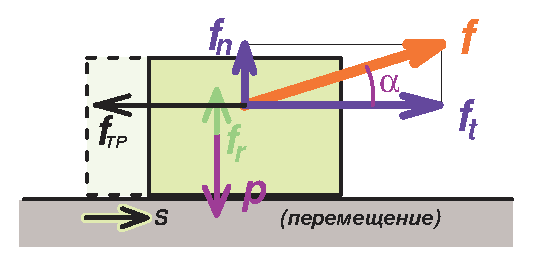
\includegraphics{GP004/GP004F01.eps}}
   \put(190,0){\makebox(0,0)[br]{\parbox{100mm}{
   \sf\Large Не вся сила {\color{red}$\vec{f}$} принимает участие в перемещении тела, а только ее составляющая в направлении перемещения ${\color{blue}\vec{f_t}}$:\hspace{5mm} $f_t=f\cdot\cos\alpha$
   \begin{displaymath}
   A=S\cdot f_t = S\cdot f\cdot\cos\alpha = \left(\vec{f}\cdot\vec{S}\right)
   \end{displaymath}
   }}}
  \end{picture}
  \caption{Баланс сил при перемещении тела.}
   \label{fig:body_move}
\end{figure}

 Здесь вертикальная составляющая $\vec{f_n}$, вес тела $\vec{p}$ и реакция опоры $\vec{f_r}$ никакой работы не производят. Сила трения $\vec{f_{TP}}$ делает {\bf отрицательную} работу, по\-скольку направлена противоположно движению: $\left(\vec{f_{TP}}\cdot\vec{S}\right)<0$.\\[1mm]

 Если сила не постоянна, а меняется во время движения:\\

 \begin{figure}[htp]
 \setlength{\unitlength}{1mm}
  \begin{picture}(190,70)(0,0)
   %\put(0,0){\framebox(190,70)[b]{}}
   \put(0,0){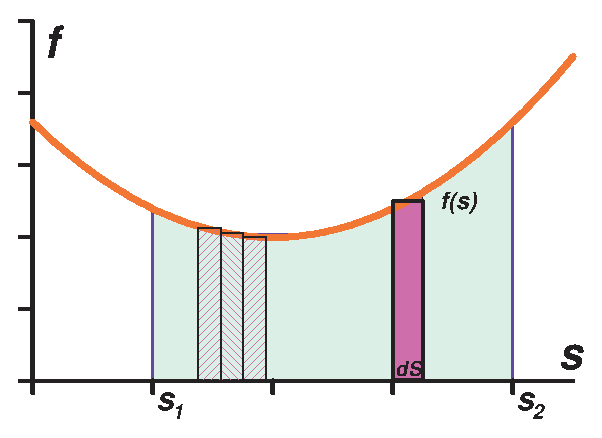
\includegraphics{GP004/GP004F02.eps}}
   \put(190,0){\makebox(0,0)[br]{\parbox{80mm}{
   \sf\Large Разобьем весь путь ($S_2-S_1$) на малые отрезки $dS$ и на каждом из отрезков посчитаем работу:
   \begin{displaymath}
   dA= \left(\vec{f}\cdot\vec{dS}\right)
   \end{displaymath}
   а затем все это просуммируем:
   \begin{displaymath}
   A=\int_{s_1}^{s_2} \left(\vec{f}\cdot\vec{dS}\right)\simeq\sum_i\left(f_i\cdot dS_i\right)
   \end{displaymath}
   }}}
  \end{picture}\\[1сm]
  \vspace{1cm}
  \begin{picture}(190,64)(0,0)
   %\put(0,0){\framebox(190,60)[b]{}}
   \put(0,0){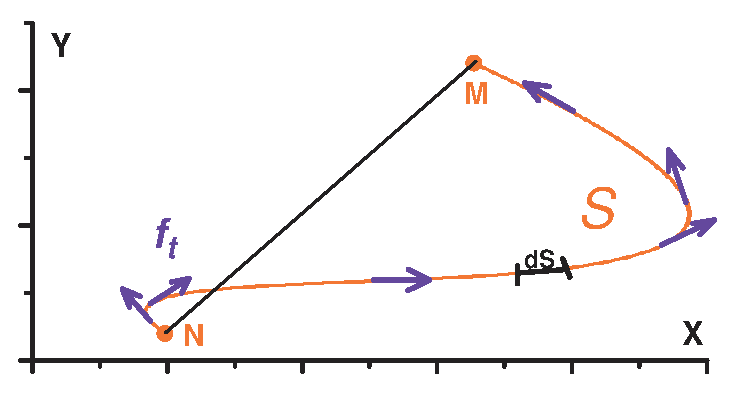
\includegraphics{GP004/GP004F03.eps}}
   \put(190,-2){\makebox(0,0)[br]{\parbox{60mm}{\sf\Large Для криволиней\-но\-го движения надо ин\-те\-гри\-ровать (сум\-ми\-ро\-вать) по пути $S$, а не по смещению $NM$:
   \begin{displaymath}
   A=\oint_{N}^{M} \left(\vec{f}\cdot\vec{dS}\right)=
   \end{displaymath}
   \begin{displaymath}
   \oint_{N}^{M} \left(f_xdx+f_ydy+f_zdz\right)
   \end{displaymath}
   }}}
  \end{picture}
  \caption{\sf\Large Интеграл работы при переменной силе (вверху) или криволинейному движении (внизу.}
   \label{fig:}
\end{figure}

\section{Мощность}

%\underline{\bf Мощность}
\begin{center}
\fbox{\parbox{180mm}{\color{blue}\bf Физ. величина, пропорциональная работе и обратно пропорциональная тому времени, за которое она совершена.}}\\[1mm]
\end{center}
Средняя мощность за промежуток времени $\Delta t$:
   \begin{displaymath}
   W=\frac{\Delta A}{\Delta t}=\frac{f\cdot \Delta S}{\Delta t}
   \end{displaymath}
Мгновенная мощность в данный момет:
   \begin{displaymath}
   W(t=\tau)=\lim_{\Delta t\rightarrow 0}\frac{\Delta A}{\Delta t}=\frac{dA}{dt}=f_t\cdot\frac{dS}{dt}=\left(\vec{f}\cdot\vec{v}\right)
   \end{displaymath}

\underline{\bf Единицы работы и мощности}
\begin{itemize}
\item CGS: $[s]$ = см, $\;\;\;\;[f]$ = дина = г$\cdot$см/с$^2$ \\ $\;\;\Rightarrow\hspace{10mm}[A]$ = эрг = г$\cdot$см$^2$/с$^2$\\
    $\;\;\Rightarrow\hspace{10mm}[W]$ = эрг/с = г$\cdot$см$^2$/с$^3$
\item SI: $\;\;\;[s]$ = м, $\;[f]$ = Ньютон (Н)= кг$\cdot$м/с$^2$ \\ $\;\;\Rightarrow\hspace{10mm}[A]$ = Джоуль (Дж) = кг$\cdot$м$^2$/с$^2 = 10^7$ эргов\\
    $\;\;\Rightarrow\hspace{10mm}[W]$ = Ватт (Вт) = кг$\cdot$м$^2$/с$^3 = 10^7$ эргов/c
\item несистемные:\\
    $\;\;\Rightarrow\hspace{10mm}[A]$ = кВт$\cdot$час = 3.6$\cdot10^6$ Дж\\
    $\;\;\Rightarrow\hspace{10mm}[W]$ = лошадиная сила (л.с.) = 736 Вт = 0.736 кВт
\end{itemize}
Пример: поезд едет с $v$=72 км/час. Мощность = ? (Рис.~\ref{fig:W_train})\\

\begin{figure}[ht]
  \begin{picture}(190,40)(0,0)
   %\put(0,0){\framebox(190,40)[b]{}}
   \put(10,0){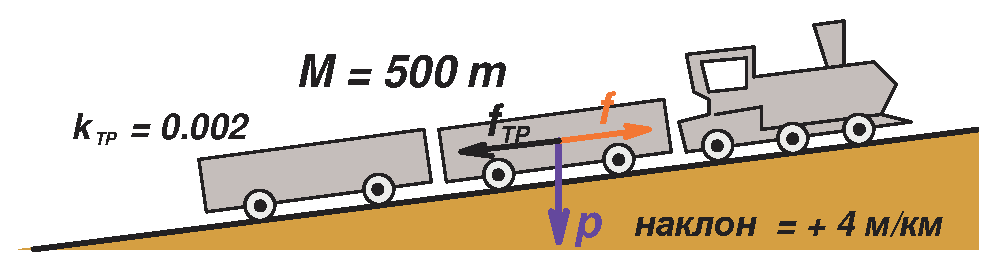
\includegraphics{GP004/GP004F04.eps}}
  \end{picture}
\caption{\sf\Large Рисунок к задаче расчета мощности поезда.}
   \label{fig:W_train}
\end{figure}
  
Решение: скатывающая сила = $p\cdot\sin\alpha\simeq p\cdot\alpha\simeq p\cdot\tan\alpha=0.004p$; она складывается с силой трения $f_{TP}=p\cdot\cos\alpha\cdot k_{TP}\simeq0.002p$.
Поскольку ускорения нет, то все силы скомпенсированы, и $f=0.006p=0.006mg=6\cdot10^{-3}\cdot5\cdot10^5$ кг$\cdot9.8$ м/с$^2=29.4$ кН. Мощность = $f\cdot v=2.94\cdot10^4\cdot72000/3600$ кг$\cdot$м$^2/c^3 = 5.88\cdot10^5$ Вт = 588 кВт $\simeq$ 0.6 МВт $\simeq$ 433 л.с.

%newpage
\section{Кинетическая энергия}

%\underline{\bf Кинетическая энергия}

Работа силы $f$ по разгону тела от $v_1$ до $v_2$ за время $t$: $A=fs$ при ускорении $a=(v_2-v_1)/t$. Сила равна $f=ma=m(v_2-v_1)/t$. Средняя скорость $\bar{v}=(v_1+v_2)/2$, поэтому расстояние $s=t\bar{v}$. Подставив, получим:
   \begin{displaymath}
   A=m\cdot\frac{v_2-v_1}{t}\cdot\frac{v_1+v_2}2\cdot t=\frac{mv_2^2}2-\frac{mv_1^2}2
   \end{displaymath}

\fbox{\parbox{170mm}{\color{blue}Работа силы $f$ численно равна приращению величины $E_k=mv^2/2$, которая называется кинетической энергией.}}\\[2mm]

Если имеется несколько материальных точек, образующих систему, то сказанное справедливо для каждой из них и для всей системы:
   \begin{displaymath}
   E_k=\sum_i\frac{m_iv_i^2}2;\;\;\;\;\;\;\;\;A=\Delta E_k
   \end{displaymath}

\fbox{\parbox{170mm}{\color{blue}Изменение кинетической энергии системы равно работе всех сил, приложенных к материальным точкам, образующим систему.}}\\[2mm]

\section{Потенциальная энергия}
%\underline{\bf Потенциальная энергия}

Силовое поле -- пространство, где на тела действуют силы. Например: однородное гравитационное поле.\\

Задача.  С горы съезжает слаломист (Рис.~\ref{fig:slalom_task}). Разобьем его трассу на короткие {\bf прямые} кусочки. Работа силы тяжести на каждом i-ом отрезке:
   $dA_i=dS_i\cdot p\cdot\cos\alpha_i$. Но ведь $dS_i\cdot\cos\alpha_i=dh_i$,
    
\begin{figure}[ht]
\centering
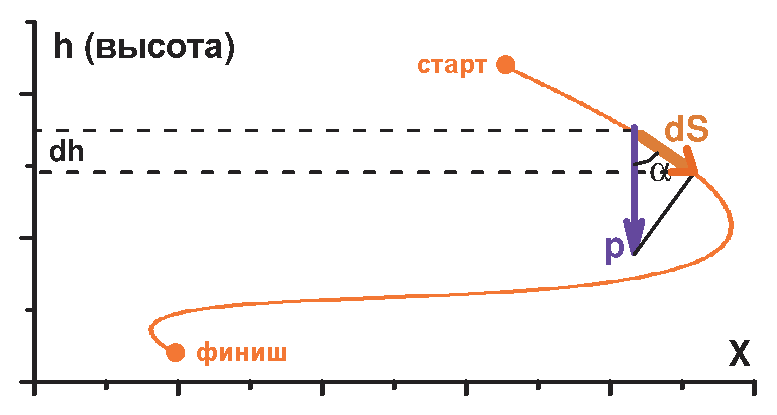
\includegraphics{GP004/GP004F05.eps}

%\begin{picture}(190,66)(0,0)
%   %\put(0,0){\framebox(190,66)[b]{}}
%   \put(0,0){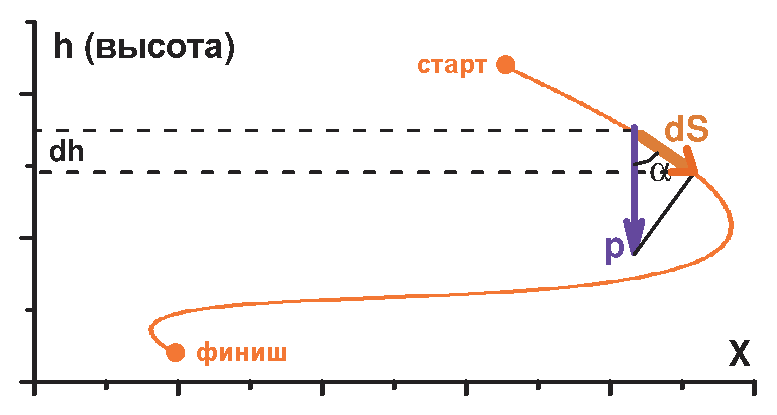
\includegraphics{GP004/GP004F05.eps}}
%  \end{picture}

  \caption{\sf\Large Задача про слаломиста.}
   \label{fig:slalom_task}
\end{figure}

поэтому вся (суммарная) работа от старта до финиша составляет
   \begin{displaymath}
   A=\sum_idA_i=\sum_ip\cdot dh_i=p\cdot\sum_idh_i=p\cdot h
   \end{displaymath}

и зависит не от формы или длины пути, а только от перепада высот! Такие силы называются потенциальными.

Введем понятие потенциальной энергии $E_p$ -- такой величины, характери\-зующей положение материальной точки в поле потенциальных сил, что работа при перемещении из одной точки поля в другую будет равна разности значений $E_{p}$ в этих точках:
   \begin{displaymath}
   A_{1,2}=E_{p1}-E_{p2}
   \end{displaymath}
Заметим, что $E_p$ -- не абсолютна, а задает только {\bf разность} по сравнению с какой-то $E_p$, условно принятой за 0.

Для тела с массой $m$ потенциальная энергия в однородном гравитационном поле равна $E_p=mgh$, где $h$ -- уровень относительно некой нулевой высоты.\\

Еще пример: сжимаем пружину с жесткостью $k$ (Рис.~\ref{fig:k_spring}).\\

\begin{figure}[ht]
    \begin{picture}(190,110)(0,0)
   %\put(0,0){\framebox(80,110)[b]{}}
   \put(0,0){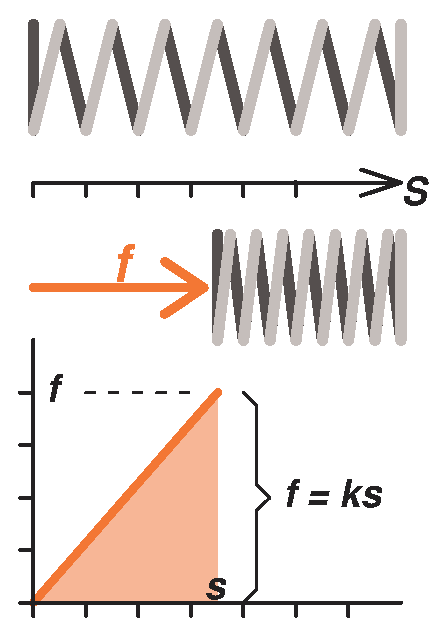
\includegraphics{GP004/GP004F06.eps}}
   \put(190,0){\makebox(0,0)[br]{\parbox{110mm}{ \sf\Large Сила непостоянна и растет: $f=ks$.  Разбивая отрезок $s$ на короткие кусочки и считая силу на каждом кусочке постоянной, получим, что совершенная работа
   \begin{displaymath}
   A=\sum_i k\cdot s_i\cdot ds_i\;\;\rightarrow\;\;S_\Delta=s\cdot ks/2 = ks^2/2
   \end{displaymath}
или через интеграл:
   \begin{displaymath}
   A=\int_0^sf(s)ds=\int_0^sks\;ds=ks^2/2
   \end{displaymath}
Сжимая пружину, {\bf мы} совершаем работу, а {\bf не пружина}, поэтому мы {\bf увеличиваем} ее потенциальную энергию: $E_p=ks^2/2$.
   }}}
  \end{picture}
  \caption{\sf\Large Задача о сжатии пружины.}
   \label{fig:k_spring}
\end{figure}

\section{Закон сохранения механической энергии}

Как и $E_k$, так же и $E_p$ системы равна сумме $E_{pi}$ частиц, составляющих эту систему. Если система изолирована и если все силы в ней -- потенциальные, то полная работа $A_{1,2}$ при переходе из состояния 1 в состояние 2 зависит только от разности начальной и конечной конфигураций системы, но не от способа перемещений:
   \begin{displaymath}
   A_{1,2}=E_{p1}-E_{p2}
   \end{displaymath}
Это же можно сказать и про разность кинетических энергий системы в состояниях 1 и 2:
   \begin{displaymath}
   A_{1,2}=E_{k2}-E_{k1}
   \end{displaymath}
Сравнивая, получим:
   \begin{displaymath}
   E_{p1}+E_{k1}=E_{p2}+E_{k2}
   \end{displaymath}

\fbox{\parbox{170mm}{\begin{center} \color{red} Закон сохранения механической энергии:\\ \color{blue}
Полная энергия изолированной системы, в которой действуют только потенциальные силы, остается постоянной.
\end{center}
}}\\[2mm]

Пусть $\exists$ замкнутая система с какой-то $E_p=E_0$ и $E_k=0$ (все тела системы покоятся). Тогда при любом движении $E_k$ увеличится ($E_k$ не может быть отрицательной). Это увеличение возможно только за счет уменьшения $E_p$. Если оказалось, что $E_p$ и так минимальна, то: \\

\fbox{\parbox{170mm}{\begin{center}\color{blue}
Замкнутая мех.система, $E_p$ которой имеет минимум и в которой отсутствует движение, находится в состоянии равновесия.
\end{center}
}}\\[2mm]

Что будет, если система неизолированная, и в ней есть трение? Силы в этой системе:
\begin{itemize}
\item внутренние потенциальные
\item внутренние непотенциальные (трение)
\item внешние
\end{itemize}
Тогда работа совершается этими тремя видами сил:
   \begin{displaymath}
   E_{k2}-E_{k1}=A_{1,2}=A_{\rm int}+A_{\rm fr}+A_{\rm ext}
   \end{displaymath}
Из ЗСЭ следует, что {\bf \color{blue} изменение полной механической энергии лю\-бой системы равно сумме работ внешних сил и сил трения}:
   \begin{displaymath}
   E_{2}-E_{1}=A_{\rm fr}+A_{\rm ext}
   \end{displaymath}
%\newpage
\underline{\bf Гравитация (силы тяготения).} \\[2mm]
\fbox{\parbox{190mm}{\begin{center} \color{red} Закон всемирного тяготения (Ньютон, 1687 г.):\\ \color{blue}
Всякие тела притягиваются друг к другу с силой,\\ прямо пропорциональной произведению их масс\\ и обратно пропорциональной квадрату расстояния между ними.
\end{center}
}}\\[2mm]
   \begin{displaymath}
   f=G\cdot\frac{m_1 m_2}{r^2}
   \end{displaymath}
Это справедливо только если $r\ll$ размера тел. В противном случе надо интегрировать:\\

\begin{figure}[ht]
  \begin{picture}(190,38)(0,0)
   %\put(0,0){\framebox(190,40)[b]{}}
   \put(0,0){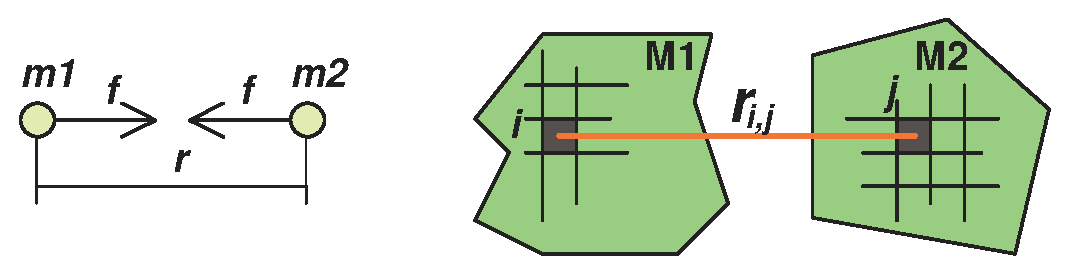
\includegraphics{GP004/GP004F07.eps}}
  \end{picture}
 \caption{\sf\Large Силы тяготения точечных (слева) и больших (справа) тел.}
   \label{fig:grav_point}
\end{figure}

разбивать каждое тело на мелкие кусочки $\Delta M$, вычислять притяжение между каждой парой кусочков  $\Delta f$ и затем все это суммировать (Рис.~\ref{fig:grav_point} справа):
   \begin{displaymath}
   f=\sum_{i,j}f_{i,j}=\sum_{i,j}G\cdot\frac{\Delta m_i\cdot\Delta m_j}{r_{i,j}^2}
   \end{displaymath}
Результат интегрирования оказывается таким же только в том случае, когда тела имеют форму однородного шара или сферы -- тогда в качестве $r$ надо просто взять расстояние между {\bf центрами} тел.\\

\underline{\bf Измерение гравитационной постоянной $G$}\\

История показана на (Рис.~\ref{fig:grav_const})

\begin{figure}[ht]
  \begin{picture}(190,60)(0,0)
   %\put(0,0){\framebox(190,60)[b]{}}
   \put(113,0){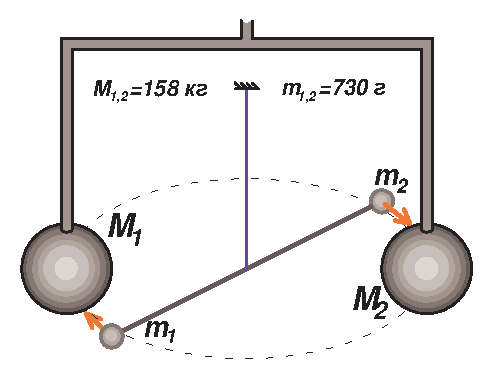
\includegraphics{GP004/GP004F08.eps}}
   \put(0,0){\makebox(0,0)[bl]{\parbox{110mm}{\sf\Large
   Дж.Мичелл (1793): крутильные весы.\\Г.Кавендиш (1798): плотность Земли\\
   С.Пуассон (1811): термин "Гравитационная постоянная"
   \begin{center}
   \fbox{$G=6.67428_{\it 67}\cdot10^{-8}$ дин см$^2$/г$^2$}
   \end{center}
   \begin{center}
   \fbox{$G=6.67428\pm0.00067\cdot10^{-11}$ Н м$^2$/кг$^2$}
   \end{center}
      }}}
  \end{picture}
  \caption{\sf\Large Гравитационная постоянная.}
   \label{fig:grav_const}
\end{figure}

%  \newpage
  У поверхности Земли ускорение тела с массой $m$, вызванное гравитацией:
  \begin{displaymath}
  g=\frac fm=G\cdot\frac{m\cdot M}{m\cdot R^2}=G\cdot\frac M{R^2}
  \end{displaymath}
  Зная $g$ и радиус Земли (из географии, начиная с Архимеда), можно определить массу Земли и ее плотность (что и делал Кавендиш):
  \begin{displaymath}
  M=\frac {g\cdot R^2}G \simeq 5.98\cdot10^{27}\texttt{г};
  \hspace{20mm}\overline{d}=\frac M{\frac43\pi R^3}\simeq5.5\;\texttt{г}/\texttt{см}^3
  \end{displaymath}
  Зная радиус $r$ орбиты Земли относительно Солнца и период ее обращения, можно найти массу Солнца, т.к. гравитация играет роль центростремительной силы:
  \begin{displaymath}
   G\cdot\frac{M\cdot M_\odot}{r^2}=M\cdot r\cdot\frac{4\pi^2}{T^2}\hspace{10mm}
   \Rightarrow\hspace{10mm}
   M_\odot=\frac{4\pi^2}G\cdot\frac{r^3}{T^2}\simeq1.98\cdot10^{33}\;\texttt{г}
  \end{displaymath}
btw: отсюда следует, что для разных планет квадраты периодов обращения относятся как кубы радиусов орбит (третий закон Кеплера).\\

Еще задачка: какой высоты д.б. орбита спутника, чтобы с Земли казалось, что он висит неподвижно (Рис.~\ref{fig:earth_sat})?
\\

\begin{figure}[ht]
  \begin{picture}(190,60)(0,0)
   %\put(0,0){\framebox(190,60)[b]{}}
   \put(0,0){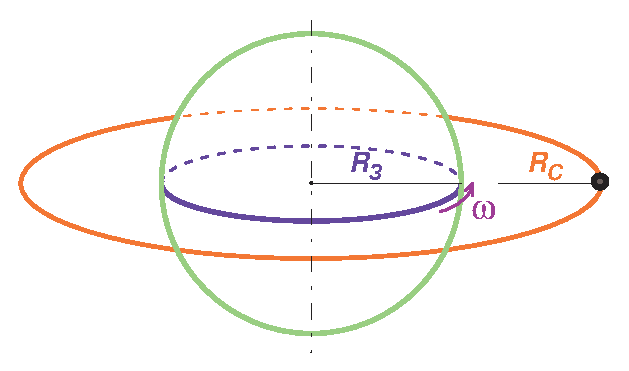
\includegraphics{GP004/GP004F09.eps}}
   \put(190,0){\makebox(0,0)[br]{\parbox{80mm}{\sf\Large 
  \begin{displaymath}
   G\cdot\frac{M\cdot m}{R_c^2}=m\cdot R_c\cdot\frac{4\pi^2}{T^2}
  \end{displaymath}
  \begin{displaymath}
   R_c^3=\frac{G\cdot M\cdot T^2}{4\pi^2}
  \end{displaymath}
  \begin{displaymath}
   \rule{0mm}{9mm}R_c\simeq\sqrt[3]{75\cdot10^{21}\texttt{м}^3}\simeq
  \end{displaymath}
  \begin{displaymath}
   \simeq4.2\cdot10^7\texttt{м}=42000\;\texttt{км}
  \end{displaymath}
  }}}
  \end{picture}\\[2mm]
\caption{\sf\Large Рисунок к задаче.}
   \label{fig:earth_sat}
\end{figure}

Какова потенциальная энергия покоящегося гравитирующего тела на $\infty$?
  \begin{displaymath}
   \left.E_{\infty}=\int\limits_R^\infty f(r)dr=\int\limits_R^\infty \frac{G\cdot M\cdot m}{r^2}dr=
   -\frac{G\cdot M\cdot m}{r}\right|_R^\infty=\frac{G\cdot M\cdot m}{R}
  \end{displaymath}
Если такое тело упадет, то вся $E_p=E_\infty$ перейдет в $E_k=mv^2/2$:
  \begin{displaymath}
   \frac{G\cdot M\cdot m}{R}=\frac{m\cdot v^2}2\hspace{10mm}\Rightarrow\hspace{10mm}
   v=\sqrt{\frac{2GM}{R}}\simeq11.2\;\texttt{км/с}
  \end{displaymath}



\chapter{Движение твердого тела}
\sf\Large


%\centerline{\underline{\Huge\bf ДВИЖЕНИЕ ТВЕРДОГО ТЕЛА}}

Как уже говорилось, любое движение = поступательное + вращение.\\
\underline{\bf Поступательное}: все точки тела имеют равные $\vec{v}$ и равные $\vec{a}$. Если мысленно разбить тело на кусочки, то $\forall \Delta m_i$ по 2зН: $\Delta m_i\cdot\vec{a}=\vec{f_i}+\vec{F_i}$, где $\vec{f_i}$ -- внутренние силы от других элементов тела, а $\vec{F_i}$ -- силы внешние. По 3зН: $\sum \vec{f_i}=0$, поэтому
\begin{displaymath}
\sum_i\Delta m_i\cdot\vec{a}=\sum_i\vec{F_i}\hspace{10mm}\Rightarrow\hspace{10mm}
\vec{a}\cdot\sum_i\Delta m_i=\sum_i\vec{F_i}\hspace{10mm}\Rightarrow\hspace{10mm}
M\cdot\vec{a}=\vec{F}
\end{displaymath}
$\vec{F}=\sum\vec{F_i}$ -- {\bf главный вектор внешних сил}.\\[2mm]
\fbox{\parbox{190mm}{\begin{center}\color{blue}
Рассмотрение поступательного движения твердого тела можно заменить рассмотрением движения одной материальной точки с массой тела, находящейся под действием главного вектора внешних сил.
\end{center}
}}\\

При более сложном (непоступательном) движении: {\bf разные} точки тела имеют {\bf разные} скорости $\vec{v_i}$ и {\bf разные} ускорения $\vec{a_i}$.

  \begin{picture}(190,45)(0,0)
   %\put(0,0){\framebox(190,40)[b]{}}
   \put(85,0){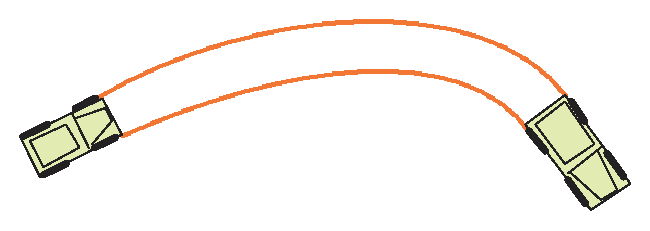
\includegraphics{GP005/GP005F01.eps}}
   \put(0,0){\makebox(0,0)[bl]{\parbox{80mm}{Пример: на этом повороте левые колеса проезжают больший путь, чем правые $\Rightarrow$ водитель движется с большей скоростью, чем пассажир!
   }}}
  \end{picture}\\[10mm]
Разбив (мысленно) тело на малые кусочки, для каждого кусочка получим:
\begin{displaymath}
 \Delta m_i\cdot\vec{a_i}=\vec{f_i}+\vec{F_i}
\end{displaymath}
Если просуммировать и учесть, что $\sum \vec{f_i}=0$, а $\sum\vec{F_i}=\vec{F}$, то
\begin{equation}
\sum_i\Delta m_i\cdot\vec{a_i}=\sum_i\vec{F_i}=\vec{F}
\end{equation}
но тут уже все $\vec{a_i}$ -- разные, и их из-под знака $\sum$ не вынести... Что делать?

\fbox{\parbox{180mm}{\begin{center}\color{blue}
{\bf Центр масс $\equiv$ центр инерции $\equiv$ центр тяжести}: ($\cdot$)C
\begin{displaymath}
x(C)=\frac{\sum x_i\cdot\Delta m_i}M\hspace{10mm}
y(C)=\frac{\sum y_i\cdot\Delta m_i}M\hspace{10mm}
z(C)=\frac{\sum z_i\cdot\Delta m_i}M
\end{displaymath}
\begin{displaymath}
x(C)=\int x\,\rho\,dV/M \hspace{10mm}
y(C)=\int y\,\rho\,dV/M\hspace{10mm}
z(C)=\int z\,\rho\,dV/M
\end{displaymath}
\end{center}
}}\\[2mm]
Если тело C состоит из частей A+B, то его центр масс совпадает со средне-взвешенным от центров масс отдельных частей:
\begin{displaymath}
\vec{r}(C) =\frac{m_A\cdot\vec{r}(A)+m_B\cdot\vec{r}(B)}{m_A+m_B}
\end{displaymath}


Ускорение центра масс $\vec{a}(C)$ по составляющим:
\begin{displaymath}
a_x(C) \equiv \frac{d^2x(C)}{dt^2}
=\frac{d^2}{dt^2}\left(\frac{\sum x_i\cdot\Delta m_i}M\right)
=\frac{\sum \Delta m_i\cdot\frac{d^2x_i}{dt^2}}M
=\frac{\sum \Delta m_i\cdot a_{ix}}M
\end{displaymath}
\begin{displaymath}
a_y(C) \equiv \frac{d^2y(C)}{dt^2}
=\frac{d^2}{dt^2}\left(\frac{\sum y_i\cdot\Delta m_i}M\right)
=\frac{\sum \Delta m_i\cdot\frac{d^2y_i}{dt^2}}M
=\frac{\sum \Delta m_i\cdot a_{iy}}M
\end{displaymath}
\begin{displaymath}
a_z(C) \equiv \frac{d^2z(C)}{dt^2}
=\frac{d^2}{dt^2}\left(\frac{\sum z_i\cdot\Delta m_i}M\right)
=\frac{\sum \Delta m_i\cdot\frac{d^2z_i}{dt^2}}M
=\frac{\sum \Delta m_i\cdot a_{iz}}M
\end{displaymath}\\
или сразу в векторном виде:
\begin{displaymath}
\vec{a}(C) \equiv \frac{d^2\vec{r}(C)}{dt^2}
=\frac{\sum \Delta m_i\cdot \vec{a}_{i}}M
\end{displaymath}

Сравнивая с (1), получаем: \hspace{10mm}$M\vec{a}(C) =\vec{F}$
\\[3mm]
\fbox{\parbox{190mm}{\begin{center}\color{blue}
Центр масс (ц.м.) тела движется так, как движется материальная точка с массой, равной массе тела, под действием силы, равной главному вектору внешних сил.
\end{center}
}}\\[1mm]

Если $\vec{F}$=0, то ц.м. покоится (или движется прямолинейно и равномерно).

Внутренние силы не могут изменить движение ц.м.
\newpage
\noindent
\begin{tabular}{|cc||cc|} \hline
\multicolumn{2}{|c||}{\rule[-5mm]{0mm}{13mm}\bf Поступательное движение} &
\multicolumn{2}{c|}{\bf Вращательное движение}\\ \hline\hline
\multicolumn{4}{|c|}{\color{blue}\bf Физические величины и понятия:\rule[-5mm]{0mm}{15mm}}\\ \hline
расстояние \rule[-5mm]{0mm}{13mm}& $s$ & угол & $\varphi$\\ \hline
координата \rule[-5mm]{0mm}{13mm}& $\vec{s}$ & угол & $\vec{\varphi}$\\ \hline
скорость \rule[-5mm]{0mm}{13mm}& $\vec{v}=\dot{\vec{s}}$ & угловая скорость & $\vec{\omega}=\dot{\vec{\varphi}}$\\ \hline
ускорение \rule[-5mm]{0mm}{13mm}& $\vec{a}=\ddot{\vec{s}}$ & угловое ускорение & $\vec{\beta}=\ddot{\vec{\varphi}}$\\ \hline
масса \rule[-5mm]{0mm}{13mm}& $m$ & момент инерции & $\mathcal{I}=mr^2$\\ \hline
кол.дв. (импульс)\rule[-5mm]{0mm}{13mm}&$\vec{p}=m\vec{v}$ & момент импульса & $\vec{\mathcal{L}}=\left[\vec{r}\times\vec{p}\right]=\mathcal{I}\vec{\omega}$ \\ \hline
сила \rule[-5mm]{0mm}{13mm}&$\vec{f}$ & момент силы & $\vec{\mathcal{M}}=\left[\vec{r}\times\vec{f}\right]$ \\ \hline
импульс силы \rule[-5mm]{0mm}{13mm}&$\vec{f}\Delta t$ & импульс момента силы & $\vec{\mathcal{M}}\Delta t$ \\ \hline
кин.энергия \rule[-5mm]{0mm}{13mm}&$E_k=\frac{mv^2}2$ & энергия вращения &
$\mathcal{E}_{\mathrm{rot}}=\frac{\mathcal{I}\omega^2}2$ \\ \hline\hline
\multicolumn{4}{|c|}{\color{blue}\bf Законы сохранения для изолированной системы:\rule[-5mm]{0mm}{15mm}}\\ \hline
импульса\rule[-5mm]{0mm}{13mm}&$\vec{p}=$const&
момента импульса&$\vec{\mathcal{L}}=$const\\ \hline\hline
\multicolumn{4}{|c|}{\color{blue}\bf Второй закон Ньютона:\rule[-5mm]{0mm}{15mm}}\\ \hline
\multicolumn{2}{|c||}{\rule[-5mm]{0mm}{13mm}$\vec{f}\Delta t = \Delta(\vec{p})$}&
\multicolumn{2}{c|}{$\vec{\mathcal{M}}\Delta t = \Delta(\vec{\mathcal{L}})$}\\ \hline
\multicolumn{2}{|c||}{\rule[-5mm]{0mm}{13mm}$\vec{f} = m\vec{a}$}&
\multicolumn{2}{c|}{$\vec{\mathcal{M}} = \mathcal{I}\vec{\beta}$}\\ \hline
\end{tabular}
  \begin{picture}(190,30)(0,0)
   %\put(0,0){\framebox(190,20)[b]{}}
   \put(45,-5){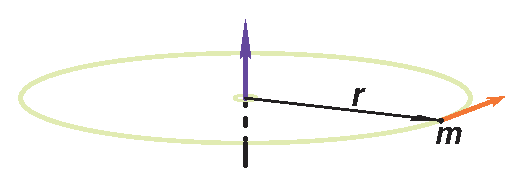
\includegraphics{GP005/GP005F02.eps}}
    \put(89,20){\makebox(0,0)[l]{\color{blue} аксиальные векторы $\vec{d\varphi}$ $\vec{\omega}$ $\vec{\beta}$ $\vec{\mathcal{L}}$ $\vec{\mathcal{M}}$}}
    \put(130,9){\makebox(0,0)[l]{\color{red} векторы $\vec{ds}$ $\vec{v}$ $\vec{a}$  $\vec{p}$ $\vec{f}$}}
  \end{picture}\\
  \begin{picture}(190,45)(0,0)
   %\put(0,0){\framebox(190,40)[b]{}}
   \put(5,0){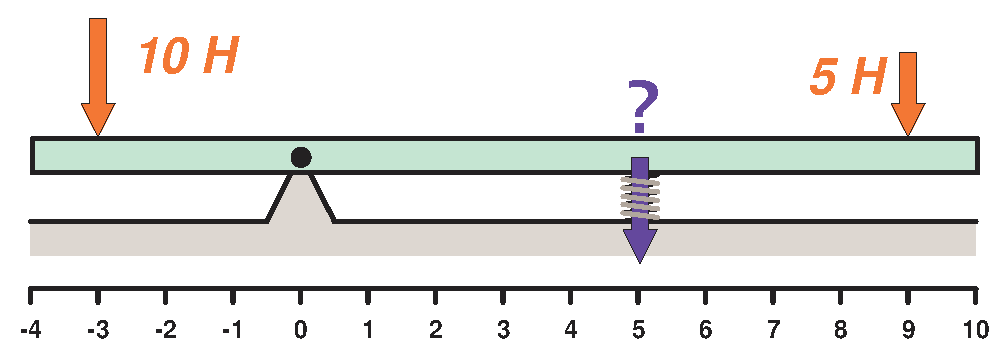
\includegraphics{GP005/GP005F03.eps}}
  \end{picture}\\
Задачка: какое усилие испытывают динамометр и ось рычага?\\
Решение: \begin{itemize}
\item момент правой силы $=\mathcal{M}_1=9\cdot5=+45$
\item момент левой силы $=\mathcal{M}_2=(-3)\cdot10=-30$
\item суммарный момент $=\mathcal{M}_\Sigma=\mathcal{M}_1+\mathcal{M}_2=+15$
\item сила на динамометре $F_\texttt{д}=\mathcal{M}_\Sigma/5=+3$ H
\item сила давления на ось $F_o=10+5-3=12$ H
\end{itemize}

Еще задачка: каков момент инерции различных простых тел?\\[2mm]
{\color{red} $\bullet$ Тонкий стержень} массой $m$ и длиной $2L$:\\
  \begin{picture}(190,20)(0,0)
   \linethickness{2mm}
   {\color{red}
   \put(30,10){\line(1,0){120}}
   }
   \put(120,10){\line(1,0){5}}
   \linethickness{0.01in}
   \put(90,10){\circle{5}}
   \put(90,10){\circle*{2}}
   \put(90,6){\vector(1,0){30}}
   \put(30,8){\makebox(0,0)[t]{\color{red}\bf -L}}
   \put(150,8){\makebox(0,0)[t]{\color{red}\bf +L}}
   \put(122,6){\makebox(0,0)[l]{$r$}}
   \put(123,12){\makebox(0,0)[b]{$dr$}}
  \end{picture}\\
Разделим стержень на кусочки. Пусть один такой кусочек длиной $dr$ находится от оси вращения на расстоянии $r$. Его масса $dm=m\cdot dr/2L$, а момент инерции $d\mathcal{I}=r^2\,dm=
mr^2dr/2L$. Момент инерции всего стержня равен
\begin{displaymath}
\mathcal{I}=2\int_0^Lm\frac{r^2dr}{2L}={\color{red}\frac{1}3mL^2}.
\end{displaymath}
{\color{red} $\bullet$  Тонкостенный цилиндр} массой $m$ и радиусом $R$:\\
  \begin{picture}(190,35)(0,0)
   %\put(0,0){\framebox(190,40)[b]{}}
   \put(0,0){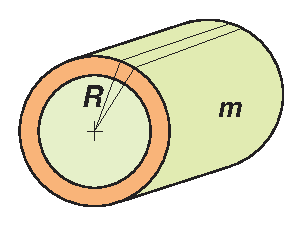
\includegraphics{GP005/GP005F04.eps}}
   \put(190,5){\makebox(0,0)[br]{\parbox{135mm}{Разобьем цилиндр на полоски с массой по $\Delta m_i$. \\
Момент инерции полоски $\Delta\mathcal{I}_i=\Delta m_iR^2$. \\
Момент инерции всего цилиндра $\mathcal{I}=\sum\Delta\mathcal{I}_i=\\ \sum\Delta m_iR^2=R^2\sum\Delta m_i=\color{red}mR^2$.
   }}}
  \end{picture}\\
{\color{red} $\bullet$  Cплошной цилиндр} представим как набор полых цилиндриков с радиусами r от 0 до R и толщинами dr. Тогда масса каждого цилиндрика будет $dm_i=m\cdot\frac{2\pi r\cdot dr}{\pi R^2}$, а суммарный момент инерции, соответственно --\vspace{-2mm}
\begin{displaymath}
\int_0^m r^2 dm = \int_0^R r^2m\frac{2 r\cdot dr}{R^2}=\frac{2m}{R^2}\int_0^Rr^3dr=\frac{2m}{R^2}\frac{R^4}4=\color{red}\frac12mR^2
\end{displaymath}
{\color{red} $\bullet$ Сфера}: разобьем ее на кольца сечением $R\,d\theta$ и длиной $2\pi h=2\pi\,R\,\sin\theta$.\\
  \begin{picture}(190,40)(0,0)
   %\put(0,0){\framebox(190,38)[b]{}}
   \put(0,0){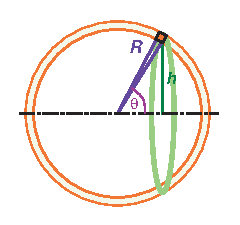
\includegraphics{GP005/GP005F05.eps}}
   \put(190,-5){\makebox(0,0)[br]{\parbox{150mm}{Площадь одного кольца $dS=2\pi R^2\sin\theta\,d\theta$, его масса $dm=m\frac{dS}S=m\,(2\pi R^2\sin\theta\,d\theta)/(4\pi R^2)=m\,\sin\theta\,d\theta/2$, а момент инерции
$d\mathcal{I}=h^2\,dm=\frac{mR^2}2\sin^3\theta\,d\theta$. Для всей сферы:\vspace{-3mm}
\begin{displaymath}
\mathcal{I}=\int_0^\pi\frac{mR^2}2\sin^3\theta\,d\theta=
\frac{mR^2}2\frac{4}3={\color{red}\frac{2}3mR^2}
\end{displaymath}
   }}}
  \end{picture}
{\color{red} $\bullet$ Однородный шар}: выделим кольцо сечением $rd\theta\times dr$ и длиной $2\pi h$=\\
\begin{picture}(190,70)(0,0)
   %\put(0,0){\framebox(190,70)[b]{}}
   \put(0,0){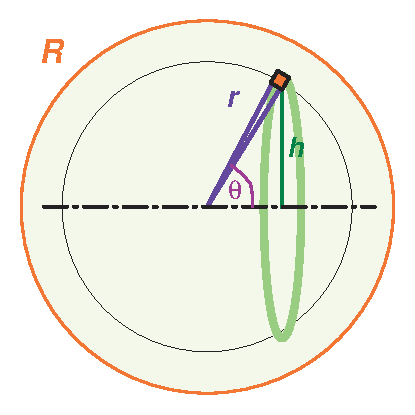
\includegraphics{GP005/GP005F06.eps}}
   \put(190,68){\makebox(0,0)[tr]{\parbox{120mm}{$=2\pi\,r\,\sin\theta$.
Объем одного такого кольца $dV=2\pi r^2\sin\theta\,d\theta\,dr$. Поскольку шар однороден, то масса кольца $dm$ пропорциональна $dV$ и равна
\begin{displaymath}
 dm=m\frac{dV}V=m\,\frac{2\pi r^2\sin\theta\,d\theta\,dr}{4\pi R^3/3},
\end{displaymath}
а момент инерции кольца $d\mathcal{I}$ составляет
\begin{displaymath}
d\mathcal{I}=h^2\,dm=m\,\frac{3 r^4\sin^3\theta\,d\theta\,dr}{2 R^3}
\end{displaymath}
   }}}
  \end{picture}\\
Чтобы получить суммарный момент инерции всего шара, надо проинтегри\-ровать $d\mathcal{I}$ по $\theta$ от 0 до $\pi$ и по $r$ от 0 до $R$:
\begin{displaymath}
\mathcal{I}=\int_0^\pi \int_0^R d\mathcal{I}=\frac{3m}{2 R^3}\int_0^\pi\sin^3\theta\,d\theta \int_0^Rr^4\,dr
\end{displaymath}
Второй из нтегралов равен $R^5/5$, а для вычисления первого сделаем замену: $x\equiv-\cos\theta$. Тогда $dx=\sin\theta$, а $\sin^2\theta=(1-x^2)$, и, как и для сферы,
\begin{displaymath}
\int_0^\pi\sin^3\theta\,d\theta = \int_{-1}^1(1-x^2)dx = \left.\left(x-\frac{x^3}3\right)\right|_{-1}^1=\frac 43
\end{displaymath}
Подставив значения обоих интегралов, получим:
\begin{displaymath}
\mathcal{I}=\frac{3mR^5\cdot4}{2 R^3\cdot5\cdot3}={\color{red}\frac 25mR^2}
\end{displaymath}
\begin{picture}(190,50)(0,0)
   %\put(0,0){\framebox(190,50)[b]{}}
   \put(0,0){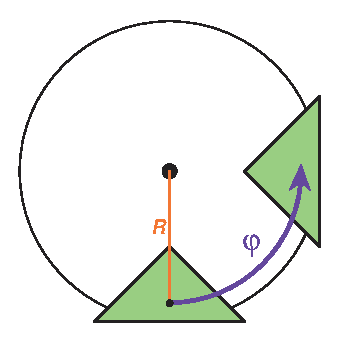
\includegraphics{GP005/GP005F07.eps}}
   \put(190,50){\makebox(0,0)[tr]{\parbox{130mm}{
   Поворот тела на угол $\varphi$ вокруг внешней оси эквивалентен поступательному движению по дуге и повороту относительно собственной оси на тот же угол $\varphi$. При этом, для поступательного движения важен только центр масс тела, а для вращения -- его собственный момент инерции $\mathcal{I}_0$.
   }}}
\end{picture}\\
\underline{Теорема Штейнера:} Момент инерции тела $\mathcal{I}$ относительно какой-либо оси равен сумме собственного момента инерции $\mathcal{I}_0$ (относительно параллельной оси, но проходящей через его центр масс) и момента инерции центра масс:
\begin{displaymath}
\mathcal{I}=\mathcal{I}_0+MR_C^2
\end{displaymath}
\begin{picture}(190,50)(0,0)
   %\put(0,0){\framebox(190,50)[b]{}}
   \put(70,0){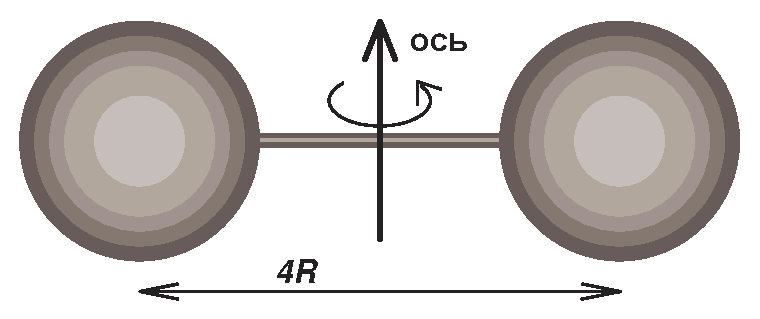
\includegraphics{GP005/GP005F08.eps}}
   \put(0,50){\makebox(0,0)[tl]{\parbox{65mm}{
   Задача: найти момент инерции гантели (2 шара радиусами $R$ и массами $M$ на расстоянии $4R$ друг от друга)
   }}}
\end{picture}\\
Решение: собственный момент инерции каждого из двух шаров $\mathcal{I}_0=MR^2\cdot2/5$, а момент инерции центра масс каждого шара относительно оси $\mathcal{I}_C=M(2R)^2=4MR^2$. Итого, в сумме получается:
\begin{displaymath}
\mathcal{I}=2\mathcal{I}_0+2\mathcal{I}_C=8.8\,MR^2
\end{displaymath}
Если гантель вращается с угловой скоростью $\omega$, то какова энергия вращения? Каждый элемент с массой $\Delta m_i$ имеет одну и ту же угловую скорость $\omega$, но линейные скорости $v_i$ будут различны: $v_i=r_i\omega$. Кинетическая энергия каждого кусочка будет $\Delta E_i=\Delta m_iv_i^2/2=\omega^2/2\cdot\Delta m_ir_i^2$, а энергия всего тела --
\begin{displaymath}
E_\texttt{rot}=\sum_i\Delta E_i=\omega^2/2\cdot\sum_i\Delta m_ir_i^2
\end{displaymath}
Но последняя сумма -- это же момент инерции! Таким образом, действительно
\begin{displaymath}
E_\texttt{rot}=\frac{\mathcal{I}\omega^2}2
\end{displaymath}

Пусть по наклонной плоскости без трения скатываются: 1) пустая бочка, 2) бочка со смолой и 3) бочка с водой. Которая скатится быстрее?

У всех потенциальная энергия $mgh$ переходит в кинетическую, состоя\-щую из энергии поступательного движения $mv^2/2$ и энергии вращения $\mathcal{I}\omega^2/2$. Для катящейся бочки ее линейная и угловая скорости связаны как $v=R\omega$, поэтому для каждой из них справедливо уравнение\vspace{-2mm}
\begin{displaymath}
mgh=\frac{mv^2}2+\frac{\mathcal{I}v^2}{2R^2}
\end{displaymath}\vspace{-2mm}
Полагая пустую бочку тонкостенным цилиндром, вспоминаем, что в этом случае $\mathcal{I}=mR^2$. Для бочки со смолой, эквиваленитной сплошному цилин\-дру, $\mathcal{I}=\frac 12mR^2$. Бочка же с водой -- это особый случай. Считая вязкость воды бесконечно малой, а массу намного большей, чем масса самой бочки, можно заявить, что вода внутри вообще не крутится, и что энергией вращения можно пренебречь.

Тогда для трех бочек получаем три разные уравнения:
\begin{displaymath}
\begin{array}{ll}
1)\rule{10mm}{0mm} mgh=\frac{mv^2}2+\frac{mv^2}2&
  \hspace{10mm}\Rightarrow\hspace{10mm}v^2=gh\\
2)\rule{10mm}{0mm} mgh=\frac{mv^2}2+\frac{mv^2}4&
  \hspace{10mm}\Rightarrow\hspace{10mm}v^2=1.5gh\\
3)\rule{10mm}{0mm} mgh=\frac{mv^2}2+0&
  \hspace{10mm}\Rightarrow\hspace{10mm}v^2=2gh
\end{array}
\end{displaymath}

\underline{\bf Гироскоп}\\
\begin{picture}(190,35)(0,0)
   %\put(0,0){\framebox(190,35)[b]{}}
   \put(0,0){\includegraphics{GP005/GP005F9a.eps}}
   \put(135,0){\includegraphics{GP005/GP005F9b.eps}}
   \put(95,35){\makebox(0,0)[t]{\parbox{65mm}{
   Приложим к гироскопу пару сил {\color{red}$\vec{F}\vec{F'}$}, создающих момент {\color{red}$\vec{M}$}. Он создаст угловое ускорение {\color{blue}$\vec{\beta}=\dot{\vec{\omega}}$},
   }}}
   \put(95,0){\makebox(0,0)[b]{которое за малый отрезок времени $\Delta t$}}
\end{picture}\\
изменит угловую скорость {\color{blue}$\vec{\omega}$} на приращение {\color{blue}$\vec{\Delta\omega}$} и тем самым повернет ось вращения вовсе не туда, куда тянули ее силы {\color{red}$\vec{F}\vec{F'}$}! Это и есть {\bf гиро\-ско\-пи\-че\-ский эффект}.

Использование: стабилизация и/или ориентация в пространстве (ги\-ро\-компасы, нарезное огнестрельное оружие, орудия в танках и на флоте, ста\-би\-ли\-зация аэрокосмических аппаратов).

{\bf Прецессия} -- круговое смещение оси вращения под действием посто\-ян\-ного опрокидывающего момента. Ядерный магнитный резонанс (ЯМР).


\chapter{Движение жидкости}
\sf\Large

%\centerline{\underline{\Huge\bf ДВИЖЕНИЕ ЖИДКОСТИ}}

\underline{\bf Сплошная среда \sl(continuum)}: непрерывное $\infty$ тело, в котором воз\-мо\-ж\-но перемещение различных частей относительно друг друга.
\begin{itemize}
\item Упругое тв. тело: относительные сдвиги, колебания
\item Несжимаемая жидкость: течения
\item Сжимаемая жидкость или газ: течения, колебания
\end{itemize}
Гидродинамика -- часть механики, изучающая движение жидкостей.\\
{\color{blue}Идеальная жидкость} -- несжимаемая и без вязкости (нет внутреннего трения)\\
  \begin{picture}(190,25)(0,0)
   %\put(0,0){\framebox(190,25)[b]{}}
   \put(135,0){\includegraphics{GP006/GP006F01.eps}}
   \put(0,22){\makebox(0,0)[tl]{\parbox{130mm}{
   {\color{blue}Поле вектора скорости}: пространство, где можно провести {\color{blue}линии тока} -- касательные к ним в каждой точке совпадают с направлением скорости частиц
   }}}
  \end{picture}\\[10mm]
  \begin{picture}(190,25)(0,0)
   %\put(0,0){\framebox(190,25)[b]{}}
   \put( 10,0){\includegraphics{GP006/GP006F2a.eps}}
   \put(100,0){\includegraphics{GP006/GP006F2b.eps}}
  \end{picture}\\[5mm]
  \begin{picture}(190,52)(0,0)
   %\put(0,0){\framebox(190,50)[b]{}}
   \put( 125,0){\includegraphics{GP006/GP006F03.eps}}
   {\color{red}
   \put(129,40){\makebox(0,0)[l]{$\Delta S_1$}}
   \put(143,35){\makebox(0,0)[l]{$\vec{v}_1$}}
   \put(183,15){\makebox(0,0)[r]{$\Delta S_2$}}
   \put(184,5){\makebox(0,0)[r]{$\vec{v}_2$}}
   }
   \put(0,52){\makebox(0,0)[tl]{\parbox{120mm}{
  Часть жидкости, ограниченная линиями тока -- {\color{blue} трубка тока}. Линии тока образуют как бы невидимые границы: частицы жидкости их не пересекают (иначе скорость была бы направлена по-другому).  }}}
   \put(0,0){\makebox(0,0)[bl]{\parbox{165mm}{
   Если в трубке тока провести 2 нормальных сечения $\Delta S_1$ и $\Delta S_2$, то за единицу времени через $\Delta S_1$ протечет объем =$\Delta S_1\cdot v_1$. Если
  }}}
  \end{picture}\\
  жидкость несжимаема, то через $\Delta S_2$ протечет столько же: $\Delta S_2\cdot v_2=\Delta S_1\cdot v_1$, и вообще для данной трубки
  \begin{displaymath}
\Delta S\cdot v=\texttt{const}\hspace{10mm}\texttt{\color{blue} -- теорема о неразрывности струи}
  \end{displaymath}

  Если $\exists$ реальная труба, то ее внутренний объем -- трубка тока. Тогда: где труба \'{у}же, там течение быстрее.
Если трубка сужается, то скорость возрастает $\Rightarrow$ есть ускорение $\Rightarrow$ есть сила! Откуда? От разности давлений. Давление в широких местах > чем в узких.

%\newpage
  \noindent
  \begin{picture}(190,60)(0,0)
   %\put(0,0){\framebox(190,60)[b]{}}
   \put( 100,0){\includegraphics{GP006/GP006F04.eps}}
   {\color{red}
   \put(110,52){\makebox(0,0)[b]{$S_1$}}
   \put(188,17){\makebox(0,0)[r]{$S_2$}}
   \put(115,40){\makebox(0,0)[l]{$\vec{v}_1$}}
   \put(186,5){\makebox(0,0)[r]{$\vec{v}_2$}}
   \color{blue}
   \put(117,47){\makebox(0,0)[r]{$p_1$}}
   \put(176,18){\makebox(0,0)[c]{$p_2$}}
   }
   \put(100,5){\makebox(0,0)[r]{$h_1$}}
   \put(170,5){\makebox(0,0)[r]{$h_2$}}
   \put(103,20){\makebox(0,0)[lb]{$h = h_1-h_2$}}
   \put(0,60){\makebox(0,0)[tl]{\parbox{90mm}{
   $S_{1,2}$ -- сечение\\
   $\vec{v}_{1,2}$ -- скорость\\
   $p_{1,2}$ -- давление\\
   $h_{1,2}$ -- высота\\
   $m$ -- порция жидкости (масса)\\
   $E_{1,2}$ -- полная энергия порции\\
   $A$ -- работа по перемещению $m$\\ от сечения 1 до сечения 2
  }}}
  \end{picture}\\
\begin{displaymath}
A=E_2-E_1,\;\;\;\;\;\;\;\;E_{1,2}=E_\texttt{кин}+E_\texttt{пот}
\end{displaymath}
\begin{displaymath}
E_1=\frac{m\cdot v_1^2}2+mgh_1\;\;\;\;\;\;\;E_2=\frac{m\cdot v_2^2}2+mgh_2
\end{displaymath}
Пусть весь столб жидкости сдвигается за время $t$ так, что через оба сечения проходит порция $m$. В точке (1) это смещение $L_1=v_1t$, а в точке (2) -- $L_2=v_2t$. Сила, толкающая жидкость в точке (1) -- это $f_1=p_1S_1$, а сила, сопротивляющаяся движению в точке (2) -- это $f_2=-p_2S_2$ (знак "минус" именно потому, что давление $p_2$ направлено навстречу движению). Работа внешних сил
\begin{displaymath}
A=f_1L_1+f_2L_2=p_1S_1v_1t-p_2S_2v_2t.
\end{displaymath}
Приравняв $A$ и $E_2-E_1$, получим:
\begin{displaymath}
\frac{m\cdot v_2^2}2+mgh_2-\frac{m\cdot v_1^2}2-mgh_1=p_1S_1v_1t-p_2S_2v_2t.
\end{displaymath}или
\begin{equation}\label{eqn.2}
 \frac{m\cdot v_1^2}2+mgh_1+p_1S_1v_1t=\frac{m\cdot v_2^2}2+mgh_2+p_2S_2v_2t.
\end{equation}
По закону неразрывности струи: $S_1v_1t=S_2v_2t$, и это -- объем $V$, занимаемый порцией $m$. Поделим ур-ние (\ref{eqn.2}) на $V$ и учтем, что $\frac mV$ -- это плотность $\rho$:
{\color{blue}
\begin{displaymath}
\frac{\rho\cdot v_1^2}2+\rho gh_1+p_1=\frac{\rho\cdot v_2^2}2+\rho gh_2+p_2.
\end{displaymath}
}
\begin{flushright}{\sl Даниил БЕРНУЛЛИ (1700-1782), СПб}\end{flushright}

%\newpage
  \noindent
  \begin{picture}(190,40)(0,0)
   %\put(0,0){\framebox(190,40)[b]{}}
   \put(20,0){\includegraphics{GP006/GP006F05.eps}}
  \end{picture}
\begin{displaymath}
\frac{\rho\cdot v_A^2}2+p_A
\hspace{7mm}=
\hspace{7mm}\frac{\rho\cdot v_B^2}2+p_B
\hspace{7mm}=
\hspace{7mm}\frac{\rho\cdot v_C^2}2+p_C
\end{displaymath}\\
\rule{189mm}{0.3mm}\\
  \begin{picture}(190,50)(0,0)
   %\put(0,0){\framebox(190,50)[b]{}}
   \put(80,0){\includegraphics{GP006/GP006F06.eps}}
   {\color{blue}
   \put(121,30){\makebox(0,0)[r]{$p_1$}}
   \put(148,30){\makebox(0,0)[r]{$p_2$}}
   }
   \put(5,45){\makebox(0,0)[tl]{\parbox{97mm}{
Скорость жидкости непосредственно перед отверстием трубки Пито $v_2=0$.
\begin{displaymath}
p_2=\frac{\rho\cdot v_1^2}2+p_1
\end{displaymath}
$p_2$ -- {\color{red} динамическое давление}
   }}}
  \end{picture}\\[2mm]
$p_1,p_2\;\;\;\Rightarrow$ измерение скорости жидкости (флот) или газа (авиация) по разности давлений.\\
\rule{189mm}{0.3mm}\\

Струйный насос:\\
  \begin{picture}(190,60)(0,0)
   %\put(0,0){\framebox(190,60)[b]{}}
   \put(0,0){\includegraphics{GP006/GP006F07.eps}}
   \put(190,60){\makebox(0,0)[tr]{\parbox{70mm}{
При достаточно большой скорости жидкости {\bf \color{green}A} на выходе из сопла давление там может стать < ат\-мо\-сфер\-но\-го, и жидкость {\bf \color{red}B} будет засасываться в струю. (жидкость $\Leftrightarrow$ газ)
   }}}
  \end{picture}\\
  \begin{picture}(190,60)(0,0)
   %\put(0,0){\framebox(190,60)[b]{}}
   \put(0,0){\includegraphics{GP006/GP006F08.eps}}
   \put(190,60){\makebox(0,0)[tr]{\parbox{130mm}{
Весь сосуд -- как одна трубка тока. Давление и у поверхности, и у отверстия = атмосферному.
Уравнение Бернулли:
\begin{displaymath}
\frac{v_1^2}2+g(h_1-h_2)=\frac{v_2^2}2
\end{displaymath}
Поскольку скорость у поверхности $\simeq0$, то получим:
\begin{displaymath}
v_2=\sqrt{2g(h_1-h_2)}=\sqrt{2gh}
\end{displaymath}
   }}}
  \end{picture}\\

Закон сохранения количества движения: струя приобрела скорость вправо; если бы система была замкнутой, то сосуд двинулся бы влево.\\ \\
  \begin{picture}(190,60)(0,0)
   %\put(0,0){\framebox(190,60)[b]{}}
   \put(0,0){\includegraphics{GP006/GP006F09.eps}}
   \put(0,51){\makebox(0,0)[l]{Пусть есть изогнутая труба постоянного сечения. За время $t$ через $S_1$ про-}}
   \put(0,43){\makebox(0,0)[l]{течет жидкость массой $m=\rho S_1v_1t$. Импульс этой массы: $\vec{p}_1=\rho S_1v_1t\vec{v}_1$.}}
   \put(190,36){\makebox(0,0)[tr]{\parbox{90mm}{
   Импульс той же массы жидкости, прходящей через $S_2$, равен $\vec{p}_2=\rho S_2v_2t\vec{v}_2$. Поскольку $S_1$=$S_2$=$S$, то и $v_1$=$v_2$=$v$, и потому $\Delta \vec{p}$ = ($\vec{p}_2$--$\vec{p}_1$)= $\rho Svt(\vec{v}_2-\vec{v}_1)$. По 2зН это должно
   }}}
  \end{picture}\\
  равняться импульсу сил, давящих на жидкость со стороны трубы: $\Delta \vec{p}$=$\vec{F}$t, и тогда, поделив на $t$, получаем:
  \begin{displaymath}
  \vec{F}= \rho Sv(\vec{v}_2-\vec{v}_1)
  \end{displaymath}
  Противоположная ей сила $\vec{F'}=-\vec{F}$ действует со стороны текущей жидкости на стенку трубы. \\
  \begin{picture}(190,45)(0,0)
   %\put(0,0){\framebox(190,45)[b]{}}
   \put(0,-5){\includegraphics{GP006/GP006F10.eps}}
   \put(190,0){\makebox(0,0)[br]{\parbox{130mm}{Пример: ветер, отражаясь от косого паруса, меняет свое направление, а сила реакции давит на парус и толкает яхту вперед. Еще пример: лопатки турбины меняют направление потока газа, а сила реакции создает момент, который крутит турбину.
   }}}
  \end{picture}
  
  %\newpage
  \section{Реактивные двигатели}
  %{\bf Реактивные двигатели.}

  По закону сохранения импульса: если газ выталкивается влево, то камера сгорания (вместе с ракетой) отталкивается вправо.

  Турбореактивные двигатели (авиация): воздух для горения берется извне и нагнетается в камеру сгорания турбиной, которую крутит сам же двигатель.

  И.В.Мещерский (1859 -- 1935): теория движения тел с переменной массой.\vspace{-3mm}
  \begin{displaymath}
  \frac d{dt}(m\vec{v})=\vec{F}+\frac{dm_1}{dt}\vec{v}_1-\frac{dm_2}{dt}\vec{v}_2
  \end{displaymath}
  Конкретно для ракеты с массой $m$ и относительной скоростью выбрасывания газов $u$:\vspace{-3mm}
  \begin{displaymath}
  m\vec{a}=\vec{F}+\frac{dm}{dt}\vec{u}
  \end{displaymath}

  К.Э.Циолковский (1857 -- 1935): характеристическая скорость $V$ -- максимальная, после выработки всего топлива.
  \begin{displaymath}
  V=I\cdot\ln\left({M_1}/{M_2}\right)
  \end{displaymath}
  $M_1$ -- начальная масса, \hspace{10mm}$M_2$ -- конечная масса\\
  $I$ -- удельный импульс $\equiv$ отношение $\frac{\texttt{тяга двигателя}}{\texttt{масса топлива за секунду}}$\\
  Выход из тупика: многоступенчатые носители.\\

\section{Движение вязкой жидкости}

%  {\bf Движение вязкой жидкости}\\
    \begin{picture}(190,37)(0,0)
   %\put(0,0){\framebox(190,37)[b]{}}
   \put(0,0){\includegraphics{GP006/GP006F11.eps}}
   \put(190,0){\makebox(0,0)[br]{\parbox{80mm}{
   Если один слой (e.g., верх\-ний) движется быстрее другого (e.g., нижнего), то между ними возникает трение (верхний тя\-нет, а нижний тормозит).
   }}}
  \end{picture}\\
  Сила внутреннего трения $f$ между слоями тем больше, чем больше площадка $\Delta S$, которую мы рассматриваем, и чем больше разница в скорости у соседних слоев (i.e., чем больше градиент скорости $\frac{dv}{dz}$):
  \begin{displaymath}
  f=\mu\frac{dv}{dz}\Delta S
  \end{displaymath}
  $\mu$ -- коэфф.внутреннего трения $\equiv$ коэффициент вязкости [Пуаз=г/см/с].\\

  \noindent
    \begin{picture}(190,90)(0,0)
   %\put(0,0){\framebox(190,90)[b]{}}
   \put(0,0){\includegraphics{GP006/GP006F12.eps}}
   \put(95,0){\includegraphics{GP006/GP006F13.eps}}
  \end{picture}\\

П.Л.Капица: сверхтекучесть гелия при T<-271C (<2.19K).

Л.Д.Ландау: гидродинамическая теория сверхтекучести.\\
\rule{189mm}{0.3mm}

До сих пор речь шла о ЛАМИНАРНОМ (слоистом) движении. Теперь поговорим о ТУРБУЛЕНТНОМ (когда вектор скорости беспордочно откло\-ня\-ется от среднего значения).\\
  \begin{picture}(190,50)(0,0)
   %\put(0,0){\framebox(190,50)[b]{}}
   \put(20,0){\includegraphics{GP006/GP006F14.eps}}
  \end{picture}\\
Поток распадается на отдельные вихри ({\bf вихрь = curl = rotor})

Число Рейнольдса R: $R=\frac{\rho v L}\mu$,  где $\rho$ -- плотность жидкости, $L$ -- ха\-рак\-тер\-ный поперечный размер (диаметр трубы, ширина или глубина реки, и т.п.). При $R>R_{\texttt{критич.}}$ происходит переход движения от ламинарного к турбулентному. Для воды в трубе $R_{\texttt{критич.}}\simeq$ 1200. Смысл R: работа сил трения по сравнению с кинетической энергией.

{\bf Закон Стокса} для шара в вязкой жидкости: $f=6\pi\mu r v$. Если учесть выталкивающую силу, то эффективный вес шара
\begin{displaymath}
P=(\rho_\texttt{ш}-\rho_\texttt{ж})g\frac43\pi r^3
\end{displaymath}
и для {\em установившейся скорости} падения шара в жидкости получим:
\begin{displaymath}
v=\frac{2(\rho_\texttt{ш}-\rho_\texttt{ж})g r^2}{9\mu}
\end{displaymath}
Закон Стокса выполняется только при малых значениях R. При больших R начинают появляться вихри, которые уносят большую энергию $\Rightarrow$ со\-про\-тив\-ле\-ние резко возрастает.

Подъемная сила. Н.Е.Жуковский (1847 -- 1921). Обтекание НЕСИМ\-МЕТ\-РИЧ\-НО\-ГО тела ВЯЗКОЙ жидкостью:\\
  \begin{picture}(190,57)(0,0)
   %\put(0,0){\framebox(190,60)[b]{}}
   \put(100,0){\includegraphics{GP006/GP006F15.eps}}
   \put(0,0){\makebox(0,0)[bl]{\parbox{90mm}{
   Давление внизу $p_B$ равно давлению во всей жидкости $p$, а вверху скорость должна возрасти, и потому давление (по формуле Бернулли) должно уменьшиться: $p_T<p$. Результирующая сила направлена вверх!
   }}}
  \end{picture}

  Если рассмотреть движение вязкой жидкости в круглой трубе, то мож\-но выделить цилиндрические слои. Быстрее всех движется самый цент\-раль\-ный, а медленнее -- прилегающий к стенке. Чем меньше радиус трубы -- тем больше поперечный градиент скорости и тем больше трение. Решая страшные уравнения, можно получить:
  \begin{displaymath}
  v=\frac{p_1-p_2}{4L\mu}(R^2-r^2)
  \end{displaymath}
  Здесь $L$ -- длина трубы, $R$ -- ее радиус, $p_1-p_2$ -- разность давлений на входе и выходе, $r$ -- радиус рассматриваемого слоя. Интегрируя по $r$ от 0 до $R$, найдем скорость прокачки -- объем в единицу времени:
  \begin{displaymath}
  \frac{dV}{dt}=\frac{(p_1-p_2)\pi \color{red}R^4}{8L\mu}\;\;\;\;\;\;-\texttt{формула Пуазейля}
  \end{displaymath}




\chapter{Элементы СТО}
\sf\Large


%\centerline{\underline{\Huge\bf Элементы СТО}}
{\sl И.Е.Иродов, Основные законы механики, глава 6}

Представления о пространстве и времени в классической (ньютоновской) механике:
\begin{enumerate}
\item Пространство -- Евклидово и имеет 3 измерения.
\item $\exists$ время, не зависящее от пространства (но его измерение связано с законами движения)
\item Размеры тел и промежутки времени одинаковы для всех систем отсчета (Ньютон: пространство и время -- абсолютны!)
\item справедлив 1зН: $\exists$ инерциальные системы, и в них $\exists$ механический принцип относительности Галилея
\item Из (1--4) вытекают преобразования Галилея:\\   \begin{picture}(180,50)(0,0)
   %\put(0,0){\framebox(180,50)[b]{}}
   \put(125,-10){\includegraphics{GP007/GP007F01.eps}}
   \put(0,0){\makebox(0,0)[bl]{\parbox{120mm}{
   Если система {\color{red}K'}
   описывается радиус-вектором {\color{green} $\vec{R}$}
   относительно системы {\color{blue}K}, то событие, опи\-сываемое
   в этой системе радиус-вектором {\color{red}$\vec{r'}$},
   будет в системе {\color{blue}K} иметь радиус-вектор \\ ${\color{blue}\vec{r}}={\color{green}\vec{R}}+{\color{red}\vec{r'}}$. При этом {\color{blue}$t$}={\color{red}$t'$} и, соответственно,
   ${\color{blue}\dot{\vec{r}}}={\color{green}\dot{\vec{R}}}+{\color{red}\dot{\vec{r'}}}$, то есть, ${\color{blue}\vec{v}}={\color{green}\vec{V}}+{\color{red}\vec{v'}}$
   или ${\color{blue}\vec{r}}={\color{green}\vec{V}}t+{\color{red}\vec{r'}}$
   }}}
  \end{picture}
\item $\exists$ механический принцип относительности Галилея
\item $\exists$ принцип дальнодействия: все взаимодействия передаются мгновенно
\end{enumerate}
\rule{190mm}{0.3mm}
Вопрос: $\exists$ ли абсолютная система отсчета? $\exists$ ли явления (не механи\-че\-с\-кие), которые отличались бы в разных инерциальных системах?

{\bf Природа света:} Считалось, что это колебания некой упругой среды наподобие воздуха ("эфир"). Но такая среда не может быть неподвижной относительно сразу всех инерциальных систем $\Rightarrow$ должна быть одна "аб\-со\-лют\-ная" система! Эфир?...

%\newpage
{\bf \underline{Опыт Майкельсона и Морли}}\\
  \begin{picture}(190,50)(0,0)
   %\put(0,0){\framebox(190,50)[b]{}}
   \put(120,0){\includegraphics{GP007/GP007F02.eps}}
   \put(0,10){\makebox(0,0)[bl]{\parbox{110mm}{
Скорость света $c\simeq$ 300 000 км/с \\
(c 1983 года $c\equiv2.99792458\times10^{8}$ м/с)\\
Орбитальная скорость Земли $V\simeq$ 30 км/с\\
$V/c\simeq10^{-4}$, и можно попытаться увидеть результат сложения скоростей $c\pm V$.
   }}}
  \end{picture}\\
  \begin{picture}(190,100)(0,0)
   %\put(0,0){\framebox(190,100)[b]{}}
   \put(0,0){\includegraphics{GP007/GP007F03.eps}}
   \put(190,93){\makebox(0,0)[rt]{\parbox{85mm}{
1887 год. Гранитная платформа, плавающая в ванне со ртутью (убирает вибрации и облегчает вращение). {\color{blue}Первый} луч проходит путь {\color{blue}$nL$} на запад и {\color{blue}$nL$} на восток, а {\color{red}второй} -- {\color{red}$nL$} на север и {\color{red}$nL$} на юг. Пусть Земля в эфире движется на юг со скоростью $V$. В лабораторной системе (л.с.): эфир движется на север. Тогда в л.с. скорость света при движении луча на север $v_N=c+V$, на юг
   }}}
  \end{picture}\\
 $v_S=c-V$, на восток и на запад $v_O=v_W=\sqrt{c^2-V^2}$. Время, потраченное на весь путь первым лучем:
 \vspace{-5mm}
 \begin{displaymath}
 \hspace{20mm}T_1=T_O+T_W=\frac{nL}{v_O}+\frac{nL}{v_W}=\frac{2nL}{\sqrt{c^2-V^2}}
  =\frac{2nL}{c\cdot\sqrt{1-(V/c)^2}}\vspace{-5mm}
 \end{displaymath}
 Время, потраченное на весь путь вторым лучем:
 \vspace{-2mm}
 \begin{displaymath}
 T_2=T_N+T_S=\frac{nL}{v_N}+\frac{nL}{v_S}=\frac{nL}{c+V}+\frac{nL}{c-V}
 =\frac{2nLc}{c^2-V^2}=\frac{2nL}{c\cdot\left(1-(V/c)^2\right)}\vspace{-2mm}
 \end{displaymath}
 Разность путей, пройденных обоими лучами \underline{\bf в эфире}:
 \begin{displaymath}
 \Delta L=cT_2-cT_1=
\frac{2nL}{\left(1-(V/c)^2\right)}-\frac{2nL}{\sqrt{1-(V/c)^2}}\simeq nL\left( V/c\right)^2
\simeq12\;\texttt{нм}
 \end{displaymath}\vspace{-2mm}
При повороте платформы на 90$^\circ$ должно $\Delta L \leftrightarrow - \Delta L$, но никакой разности хода $2\Delta L\simeq0.04\lambda$ обнаружено не было!\\
Могло, конечно, {\bf случайно} оказаться, что в тот момент было V=0. Тогда через полгода должно быть V=60 км/с. Повторили -- безрезультатно!

Выводы: 1) эфир никак не обнаружить  2) Скорость света не зависит от скорости источника.

Максвелл: скорость распространения эл.-маг. поля в пустоте c=const безотносительно к системам отсчета(?!)

Лоренц (1892): сокращение длины тела в направлении движения.

Пуанкаре (1905): принцип относительности Галилея надо рас\-про\-стра\-нить на {\bf все явления, включая электродинамику}, а не только на механику. "Преобразования Лоренца". Одновременность событий не абсо\-лют\-на. 4-мерный интервал $r^2+(ict)^2$ -- инвариант преобразований Лоренца. Скорость распространения гравитации в эфире = с.

Эйнштейн (1905): Зачем эфир, если он ненаблюдаем? 2 постулата: спец. принцип относительности и постоянство с.

Планк (1906) и Эйнштейн (1907): релятивистская динамика и тер\-мо\-ди\-на\-мика.

Минковский (1907): математическая модель СТО (геометрия 4-мер\-но\-го псевдоевклидова пространства.

Эйнштейн (1911-1916): ОТО (гравитация как проявление кривизны пространства-времени).

Неужели нельзя разогнать что-то до скорости >c? Эксперимент Бер\-тоц\-ци на ускорителе электронов Ван-де-Граафа:\\
  \begin{picture}(190,80)(0,0)
   %\put(0,0){\framebox(190,30)[b]{}}
   \put(10,40){\includegraphics{GP007/GP007F04.eps}}
   \put(10,0){\includegraphics{GP007/GP007F05.eps}}
  \end{picture}\\


\underline{\bf ПОСТУЛАТЫ Эйнштейна} (он сложил их вместе):
\begin{enumerate}
\item Справедлив принцип относительности Эйнштейна -- расширение прин\-ци\-па Галилея.
\item Скорость света не зависит от скорости источника во всех инерциальных системах.
\item Пространство и время однородны; пространство -- изотропно.
\end{enumerate}
Если пренебречь гравитацией (а это учитывается в ОТО), то СТО выпол\-ня\-ет\-ся с точностью не хуже $10^{-12}$.\\

Раз c=const, то преобразования Галилея для скоростей НЕ ВЕРНЫ.\\
  \begin{picture}(190,45)(0,0)
   %\put(0,0){\framebox(190,40)[b]{}}
   \put(70,0){\includegraphics{GP007/GP007F06.eps}}
   \put(0,0){\makebox(0,0)[bl]{\parbox{65mm}{
   На тележке, едущей впра\-во, вспыхивает лампочка. В системе тележки свет до фотоэлементов A и B доходит одновременно.
   }}}
  \end{picture}

В л.с. пока свет летит, фотоэлемент A к нему приблизится и поймает сигнал раньше, чем B.

 То есть, ОДНОВРЕМЕННОСТЬ событий -- тоже относительна!

 Рассмотрим систему $K'$, движущуюся относительно покоящейся сис\-темы $K$ со скоростью $V$ в направлении оси $x$.

 Вместо преобразований Галилея $\Rightarrow$ преобразования Лоренца.
 \begin{displaymath}
 \begin{array}{lc|cl}
 x'=x-Vt &&\hspace{5mm}& x'=\frac{x-Vt}{\sqrt{1-V^2/c^2}}\rule[-5mm]{0mm}{10mm}\\
 y'=y    &&& y'=y\\
 z'=z    &&& z'=z\\
 t'=t    &&& t'=\frac{t-Vx/c^2}{\sqrt{1-V^2/c^2}}\rule[-6mm]{0mm}{15mm}\\ \hline
 \texttt{длина r}&&&\texttt{интервал s}\\
 r^2=x^2+y^2+z^2&&&s^2=-c^2t^2+x^2+y^2+z^2\\ \hline
 \texttt{пространство \{x,y,z\} + время \{t\}}&&&\texttt{4-континуум \{ict,x,y,z\}}
 \end{array}
 \end{displaymath}\\
  \begin{picture}(190,45)(0,0)
   %\put(0,0){\framebox(190,45)[b]{}}
   \put(0,0){\includegraphics{GP007/GP007F07.eps}}
   \put(190,0){\makebox(0,0)[br]{\parbox{100mm}{
    Пусть в двух системах есть по вер\-ти\-каль\-ному стержню одинаковой длины ($OA\!\parallel\! y$) и ($O'A'\!\parallel\! y'$). Совпадают ли их длины с точки зрения другой системы? Да. Когда системы в какой-то момент поравняются, мы это увидим. $\Rightarrow {\color{blue}y}={\color{red}y'}$.
   }}}
  \end{picture}

  \centerline{\fbox{\bf\color{blue}Поперечные размеры Лоренц-инвариантны }}
  \vspace{5mm}
  Теперь превратим стержень в "световые часы": свет бегает вдоль стержня, отражаясь от концов, а мы считаем число пробегов.\\
  \begin{picture}(190,50)(0,0)
   %\put(0,0){\framebox(190,50)[b]{}}
   \put(0,0){\includegraphics{GP007/GP007F08.eps}}
   \put(190,0){\makebox(0,0)[br]{\parbox{92mm}{
    В движущейся системе длина од\-но\-го пробега $L\!=\!(O'A')$, и он занимает время $t'=L/c$. С точки же зрения покоящейся системы, вместо катета $L$ надо брать диагональ $N$, и про\-бег займет большее время $t\!=\!\frac Nc$, причем
   }}}
  \end{picture}
  \begin{displaymath}
  \left(Vt\right)^2+L^2=(ct)^2\hspace{10mm}\Rightarrow\hspace{10mm}
  t=\frac{t'}{\sqrt{1-\left(V/c\right)^2}}\hspace{10mm}\Rightarrow\hspace{10mm}
  {\color{blue}t}\geq {\color{red}t'}
  \end{displaymath}
\\
  \centerline{\fbox{\bf\color{blue}Движущиеся часы идут медленнее, чем покоящиеся}}
  \begin{picture}(190,80)(0,0)
   %\put(0,0){\framebox(190,80)[b]{}}
   \put(70,0){\includegraphics{GP007/GP007F09.eps}}
   \put(0,0){\makebox(0,0)[bl]{\parbox{65mm}{
    Покоящийся мюон живет $\tau\!\simeq\!2$ мкс; за это время он не смог бы пролететь более 600 метров, даже двигаясь с $V\!\simeq\! c$. Од\-на\-ко, рождающиеся на высоте 20-30 км мюоны легко достигают земной поверхности и вредят экспериментаторам...
    }}}
  \end{picture}
\\
  \begin{picture}(190,55)(0,0)
   %\put(0,0){\framebox(190,55)[b]{}}
   \put(0,0){\includegraphics{GP007/GP007F10.eps}}
   \put(185,0){\makebox(0,0)[br]{\parbox{120mm}{
   Пусть теперь самолет движется вдоль оси $x$. В покоящейся системе поставим пограничный столб с часами и засечем время $t$ между моментами, когда со столбиком поравняются сначала кокпит, а затем киль самолета. Тогда его длина для стоящего возле столба погранич-
    }}}
  \end{picture}
\\
ника покажется равной $L=Vt$. У пилота нет возможности вылезти на лету и измерить длину своей машины, но он связался по рации с пограничником и узнал о показаниях часов. Будучи достаточно образован\-ным, пилот знает об эффекте замедления времени, а также о полном равноправии систем отсчета. Поэтому он считает, что часы пограничника идут медленнее (ведь они вместе со столбом движутся назад относительно самолета!) в $1/\sqrt{1-\left(V/c\right)^2}$ раз. Во столько же раз длина самолета оказыва\-ется больше с точки зрения пилота, чем это показалось пограничнику.\\
  \centerline{\fbox{\bf\color{blue} Размеры тела сокращаются в направлении движения}}
\vspace{1mm}

Попробуем вывести преобразования Лоренца для перехода от инерци\-аль\-ной системы $K$ к движущейся относительно нее вдоль оси $X$ со скорос\-тью $V$ инерциальной системе $K'$. Пространство и время однородны $\Rightarrow$   единица длины и единица времени одинаковы в любой точке пространства и в любой момент времени $\Rightarrow$ преобразования должны быть линейны:\vspace{-1mm}
\begin{equation}\label{Eq.1}
\left\{ \begin{array}{ccc}
        x'&=&Ax+Bt\\
        t'&=&Mx+Nt
        \end{array}\right.\hspace{10mm}\rightarrow\;\;\;\texttt{Найдем}\;\;\;\; A,B,M,N
\vspace{-2mm}\end{equation}\vspace{-2mm}
Перемещение вдоль оси $X$ в системе $K'$:\vspace{-2mm}
\begin{displaymath}
\Delta x'=x'_2-x'_1=A(x_2-x_1)+B(t_2-t_1)=A\Delta x+ B\Delta t
\end{displaymath}\vspace{-2mm}
Промежуток времени в системе $K'$:\vspace{-2mm}
\begin{displaymath}
\Delta t'=t'_2-t'_1=M(t_2-t_1)+N(x_2-x_1)=M\Delta x+ N\Delta t
\end{displaymath}\vspace{-2mm}
Учитывая, что скорости $v$ и $v'$ относительно систем $K$ и $K'$, соответственно, равны $v={\Delta x}/{\Delta t}$ и $v'={\Delta x'}/{\Delta t'}$, получим:\vspace{-2mm}
\begin{equation}\label{Eq.2}
v'=\frac{\Delta x'}{\Delta t'}=\frac{A\Delta x+ B\Delta t}{M\Delta x+ N\Delta t}=\frac{Av+B}{Mv+N}
\end{equation}
Рассмотрим некоторые частные случаи. Например, точка покоится в сис\-теме $K'$. Тогда $v'$=0, $v$=$V$. Подставив это в (\ref{Eq.2}), получим:
\begin{equation}
0=\frac{AV+B}{MV+N}\hspace{10mm}\Rightarrow\;\;\;\fbox{$B=-AV$}
\end{equation}
Пусть теперь точка покоится в системе $K$. Тогда $v$=0, $v'$=$-V$. Подставим в (\ref{Eq.2}):\vspace{-4mm}
\begin{equation}
-V=\frac{A\cdot0+B}{M\cdot0+N}=\frac BN=-\frac{AV}N\hspace{10mm}\Rightarrow\;\;\;\fbox{$N=A$}
\end{equation}
Теперь пусть в системе $K'$ распространяется свет. Тогда $v'$=$v$=$c$. Под\-ста\-вим в (\ref{Eq.2}):\vspace{-4mm}
\begin{equation}
c=\frac{Ac-AV}{Mc+A}\hspace{10mm}\Rightarrow\;\;\;\fbox{$M=-AV/c^2$}
\end{equation}
С учетом всего этого, формула (\ref{Eq.2}) превращается в\\[3mm]
{\color{blue} \parbox{180mm}{
\centerline{\fbox{\bf формулу сложения скоростей:}}
\begin{displaymath}
v'=\frac{v-V}{1-\frac{vV}{c^2}}\hspace{20mm}v=\frac{v'+V}{1+\frac{v'V}{c^2}}
\end{displaymath}
}}\\
\fbox{\parbox{190mm}{\sl Пример: две частицы летят навстречу друг другу со скоростями $+\frac 34c$ и $-\frac 34c$. Какова их встречная скорость? Свяжем систему $K'$ с первой частицей ($V=+\frac 34c$). Тогда с точки зрения этой первой частицы, скорость второй будет вовсе не $(\frac 34+\frac 34)c=1.5c$, а
\vspace{-3mm}
\begin{displaymath}
v'=\frac{-\frac 34c-\frac 34c}{1-\frac{-9c^2}{16c^2}}=\frac{-\frac 32 c}{\frac{25}{16}}=
-\frac{24}{25}c=-0.96c
\end{displaymath}}
\vspace{-3mm}
}\\[5mm]
\noindent
Теперь подставим найденные значения $B,M,N$ в изначальные ф-лы (1)
\vspace{-2mm}
\begin{displaymath}
\left\{ \begin{array}{ccc}
        x'&=&A(x-Vt)\\
        t'&=&A\left(t-\frac{Vx}{c^2}\right)
        \end{array}\right.
\end{displaymath}
Поскольку пространство изотропно, то можно считать, что не $K'$ движется со скоростью $V$, а $K$ движется со скоростью $-V$. Тогда получим
\vspace{-2mm}
\begin{displaymath}
\left\{ \begin{array}{ccc}
        x&=&A(x'+Vt)\\
        t&=&A\left(t'+\frac{Vx'}{c^2}\right)
        \end{array}\right.
\end{displaymath}
\vspace{-2mm}

%\newpage

"скрестив" эти четыре равенства, получим уравнение для $A$:
\begin{displaymath}
x=A^2\left(x-Vt+Vt-\frac{V^2x}{c^2}\right)=xA^2\left(1-\frac{V^2}{c^2}\right)
\end{displaymath}
Поделив это на $xA^2$, найдем значение $A$:\\
\centerline{
\fbox{\parbox{170mm}{
\vspace{-2mm}
\begin{displaymath}
A={\color{blue}\frac 1{\sqrt{1-\frac{V^2}{c^2}}}}\;\;\;\;\;\equiv\;\;\;\;\; {\color{blue}\gamma}\;\;\;\;\;\equiv\;\;\;\;\;{\color{blue}\texttt{Лоренц-фактор}}\geq 1
\vspace{-2mm}
\end{displaymath}
}}}
С учетом этого, видим, что равенства  представляют собой не что иное как преобразования Лоренца (что и требовалось)!\\

Хотя одновременность событий и относительна, но {\bf причинно-след\-ствен\-ная связь} преобразованиями Лоренца не нарушается. Причина и следствие: причина всегда раньше, и без нее следстве невозможно.

Причина: в момент времени $t_1$ в точке $x_1$ произведен выстрел. След\-ствие: в момент $t_2$ в точке $x_2$ пуля со скоростью $v$ пробивает мишень.\\
  \begin{picture}(190,38)(0,0)
   %\put(0,0){\framebox(190,35)[b]{}}
   \put(15,0){\includegraphics{GP007/GP007F11.eps}}
   \put(95,15){\makebox(0,0)[b]{$v=(x_2-x_1)/(t_2-t_1)$}}
  \end{picture}
\\
Предположим, что есть какая-то система отсчета $K'$, движущаяся со ско\-ростью $V$. В ней интервал между выстрелом и попаданием
\begin{displaymath}
 \Delta t'=t'_2-t'_1=\frac{t_2-t_1-\frac{V}{c^2}(x_2-x_1)}{\sqrt{1-(V/c)^2}}=
 (t_2-t_1)\frac{1-\frac{vV}{c^2}}{\sqrt{1-(V/c)^2}}=\Delta t\cdot\xi
\end{displaymath}
Поскольку $|v|\leq c$ и $|V|< c$, то множитель $\xi$ всегда положителен, $\Rightarrow$ знаки $\Delta t'$ и $\Delta t$ совпадают, то есть, действительно не найдется такой инерциальной системы, по отношению к которой причина и следствие поменялись бы местами.\\

\underline{\bf Интервал} $s$ между событиями 1 и 2:
\begin{displaymath}
s_{12}^2\equiv x^2+y^2+z^2-c^2t^2 = L^2-c^2t^2,
\end{displaymath}
где $L$ -- расстояние, а $t$ -- время между событиями 1 и 2. В системе $K'$:
\begin{displaymath}
s'^2=x'^2+y'^2+z'^2-c^2t'^2 =
\frac{(x-Vt)^2}{1-V^2/c^2}+y^2+z^2-
\frac{c^2(t-Vx/c^2)^2}{1-V^2/c^2}=
\end{displaymath}
\begin{displaymath}
=\ldots=
\frac{(x^2-c^2t^2)(1-V^2/c^2)}{1-V^2/c^2}+y^2+z^2=s^2
\end{displaymath}
\centerline{\fbox{\bf\color{blue}
Преобразования Лоренца не меняют длину интервала
}}
\vspace{2mm}\\
В чем смысл интервала? Лучше всего представить дело так, что вместо 3 пространственных осей ($X,Y,Z$) и одной временн\'{о}й оси ($T$), существуют 4 равноправные взаимно-ортогональные обобщенные оси $X_0,X_1,X_2,X_3$, причем обобщен\-ные координаты любого события записываются как 4-мерный вектор $\vec{x}$ с составляющими $x_\mu$ ($\mu=0\ldots3$):
\begin{equation}\label{Eq.Int}
 \vec{x}=\left\{\begin{array}{c}
                 x_0\\ x_1\\ x_2\\ x_3
                \end{array}\right\}=
\left\{\begin{array}{c}
                 ict\\ x\\ y\\ z
                \end{array}\right\};\;\;\;\;\;\;\;|x|^2 = \sum_{\mu=0}^3x_\mu^2
\end{equation}
Забыв на время об $y$- и $z$-составляющих, нарисуем "диаграмму Минковского".
\\
  \begin{picture}(190,91)(0,0)
   %\put(0,0){\framebox(190,90)[b]{}}
   \put(105,0){\includegraphics{GP007/GP007F12.eps}}
   \put(0,90){\makebox(0,0)[tl]{\parbox{100mm}{
   Начало координат -- это мы, то есть, {\bf здесь} ($x$=0) и {\bf сейчас} ($t$=0). Все остальные точки -- это события, ко\-то\-рые были ($t$<0) и будут ($t$>0) в разных закоулках Вселенной. Диагонали -- мировые линии света от нашей лампочки. Прямая $AB$ -- мировая линия покоящегося объекта. Он сможет получить нашу телеграмму только на участке $NB$.  $POQR$ -- другой объект приблизился, побудет в гостях и удалится обратно.
   }}}
  \end{picture}
\\
{\sl (Ч.Киттель, В.Найт, М.Рудерман. Берклеевский Курс Физики. Механика.)}
\\
  \begin{picture}(190,90)(0,0)
   %\put(0,0){\framebox(190,90)[b]{}}
   \put(0,0){\includegraphics{GP007/GP007F13.eps}}
   \put(190,90){\makebox(0,0)[tr]{\parbox{120mm}{
   Если теперь вспомнить еще об одной про\-стран\-ственной координате ($y$), то вместо плоской ди\-а\-грам\-мы получается световой конус. Его по\-верх\-ность -- свет. Если что-то произошло раньше (ниже плоскости $t$=0), то любая информация об этом попадет к нам не раньше, чем до\-йдет свет. Так, если событие было внутри ни\-ж\-ней части конуса, то какие-то отголоски уже могли, в принципе, до нас докатиться. Если мы что-нибудь отправим (посылку, ракету, радиограмму), то адресат имеет шанс получить послание только внутри верхнего конуса.
     }}}
  \end{picture}
   Вне конуса (то есть, при $c|t_{12}|<|L_{12}|$) не может быть причинно-след\-ствен\-ной связи. Это значит, что мы никак не можем повлиять на исход завтрашних выборов на планетах $\alpha$ Центавра (слишком далеко). Да и узнать результат этих выборов мы сможем только через 4 года. К тому моменту Центаврияне, как и мы, сдвинутся по оси $ct$ и снова окажутся вне досягаемости, но та точка, где и когда они шли к избирательным урнам, окажутся внутри нижнего конуса относительно нас. А вот послать наши рекомен\-дации к следующим выборам -- наше право.

\section{Релятивистская динамика}   
%   \centerline{\LARGE\bf \underline{РЕЛЯТИВИСТСКАЯ ДИНАМИКА}}

   Мы уже видели из эксперимента Бертоцци, что разгоняя частицу внешней силой и добавляя ей импульс, мы не увеличиваем ее скорость. $\Rightarrow$ 2зН не работает!
   Если рассмотреть процесс упругого соударения двух одинаковых шаров и применить к ним преобразования Лоренца, то можно показать, что при переходе в движущуюся систему закон сохранения импульса тоже нарушается. Это -- из-за сокращения времени.

   Оказывается, что все хорошо, если за импульс принять не $m\vec{v}$, а более сложное выражение:
  \begin{equation}
  \vec{p}=\frac{m\vec{v}}{\sqrt{1-v^2/c^2}} =m\vec{v}\gamma
  \end{equation}
   $\exists$ 2 вариант поведения: считать, что, как и раньше, \fbox{$\vec{p}=M\vec{v}$}, но под  $M$ понимать не массу покоя $m$, а релятивистскую массу
  \begin{equation}\label{Eq.M}
  M\equiv\frac{m}{\sqrt{1-v^2/c^2}} =m\gamma
  \end{equation}
Теперь понятно, почему электроны не разогнать -- их масса (\ref{Eq.M}) с ростом скорости тоже растет, и сила для разгона нужна все больше и больше!

Составим тождество
\begin{displaymath}
\frac{1}{1-v^2/c^2}-\frac{v^2/c^2}{1-v^2/c^2}=1\hspace{10mm}\texttt{или}\hspace{10mm}
\gamma^2-\beta^2\gamma^2=1
\end{displaymath}
Поскольку 1 всегда = 1 независимо от системы координат, то левая часть этого тождества -- Лоренц-инвариантна. Домножим на $m^2c^4$:
\begin{displaymath}
 m^2c^4(\gamma^2-\beta^2\gamma^2)=m^2c^4
\end{displaymath}
Учитывая, что $p^2=m^2c^2\beta^2\gamma^2$, получим: \fbox{$M^2c^4-p^2c^2=m^2c^4$}.
Поскольку масса покоя $m$ постоянна, то и $m^2c^4$ тоже постоянна $\Rightarrow$ Лоренц-инвариантна $\Rightarrow$ это равенство имеет самостоятельный физический смысл. Какой? Вспом\-нив, что $M=m\gamma=m(1-\beta^2)^{-1/2}$, разложим величину $Mc^2$ в ряд:\vspace{-2mm}
\begin{displaymath}
 Mc^2=mc^2(1-\beta^2)^{-1/2}\simeq mc^2 \left(1+\frac {\beta^2}2+\ldots\right)=
 mc^2+\frac{mv^2}2+\ldots
\end{displaymath}
Очень похоже на сумму кинетической энергии и еще чего-то, правда? Если мы определим полную релятивистскую энергию свободной частицы как
\begin{displaymath}
 W\equiv Mc^2\equiv \frac{mc^2}{\sqrt{1-v^2/c^2}} =m\gamma c^2
\end{displaymath}\vspace{-5mm}
то получим:
\begin{displaymath}
W^2-(pc)^2=\left(mc^2\right)^2
\end{displaymath}
Поскольку, как мы видели, это равенство Лоренц-инвариантно, то при переходе от одной системы $K$ к другой $K'$ и при замене $p\rightarrow p'$, $W\rightarrow W'$ должно соблюдаться
%\begin{displaymath}
\fbox{$W^2-(pc)^2=W'^2-(p'c)^2=\left(mc^2\right)^2$}
%\end{displaymath}

Вспомним о нашем определении 4-мерного интервала (\ref{Eq.Int}) и продиф\-фе\-рен\-ци\-руем его по $t$, получив 4-мерную скорость $\vec{U}$:
\begin{equation}
\frac{\partial}{\partial t}(\vec{s}) = \vec{U}=\left\{
\begin{array}{c}
ic\\ v_x\\ v_y\\ v_z
\end{array}
\right\}=\left\{
\begin{array}{c}
ic\\ \vec{v}
\end{array}
\right\}
\end{equation}
домножив на $M=m\gamma$, получим 4-мерный импульс $\vec{P}$:
\begin{equation}\label{Eq.4p}
 \vec{P}=M\vec{U}=\left\{\begin{array}{c}
                 P_0\\ P_1\\ P_2\\ P_3
                \end{array}\right\}=
\left\{\begin{array}{c}
                 icM\\ Mv_x\\ Mv_y\\ Mv_z
                \end{array}\right\}
=\left\{
\begin{array}{c}
icM\\ \vec{p}
\end{array}
\right\}
;\;\;\;\;\;\;\;|P|^2 = \sum_{\mu=0}^3P_\mu^2
\end{equation}
домножив на $c^2$, получим знакомое выражение:
\begin{equation}
|Pc|^2=p^2c^2-M^2c^4=(pc)^2-W^2
\end{equation}
А это, как мы знаем, должно с точностью до знака равняться массе покоя $mc^2$.
Кстати, знак -- дело соглашения, у разных авторов он определен по-разному.
Таким образом, 4-мерный импульс содержит в себе сразу и наш обычный (нормальный) импульс $\vec{p}$, и полную энергию объекта $W$
\begin{displaymath}
 \vec{P}=
\left\{\begin{array}{c}
                 iW/c\\ p_x\\ p_y\\ p_z
                \end{array}\right\}
=\left\{
\begin{array}{c}
iW/c\\ \vec{p}
\end{array}
\right\}
\end{displaymath}
При рассмотрении релятивистских ситуаций это очень удобно, поскольку позволяет "сэкономить" на законах сохранения -- вместо сохранения энер\-гии и сохранения импульса можно учитывать только сохранение 4-импуль\-са (отдельно по каждой составляющей). При переходе к другой системе координат отдельные компоненты 4-импульса будут меняться, но модуль останеся равным $-mc^2$. То есть, масса покоя -- Лоренц-инвариантна.

\newpage
\underline{\bf Основные формулы механики релятивистских частиц}

\sf\large

\begin{itemize}
 \item Энергия массы покоя (в системе, где частица покоится): \fbox{$mc^2$}, где $m$ -- масса покоя (часто обозначается как $m_0$). Поскольку $\forall$ частицы $mc^2$ так же постоянна, как и просто $m$, то удобнее массу частиц приводить не в граммах или килограммах, а в специфических единицах энергии. Если электрон прошел разность потенциалов 1 Вольт, то его энергия изменилась на 1 эВ (электрон-Вольт).
     
     Примеры массы покоя некоторых частиц: \begin{itemize}
     \item электрон: $m_e=0.510998910_{13}$ МэВ$/c^2$ $\simeq511$ кэВ$/c^2$
     \item мюон: $m_\mu=105.658369_{9}$ МэВ$/c^2$ $\simeq105$ МэВ$/c^2$
     \item протон:  $m_p=938.272013_{23}$ МэВ$/c^2$ $\simeq938$ МэВ$/c^2$
     \item нейтрон: $m_n=939.565530_{38}$ МэВ$/c^2$ $\simeq940$ МэВ$/c^2$
     \item фотон: $m_\gamma\equiv0$
     \item нейтрино: $m_\nu\leq 2$ эВ$/c^2$ ($\stackrel{?}{\equiv}0$  -- работаем над этим...)
     \end{itemize}
 \item Скорость частицы $\vec{v}$ в долях от скорости света: \fbox{$\beta=v/c$}     
 \item Лоренц-фактор: \fbox{$\gamma=\frac{1}{\sqrt{1-v^2/c^2}}=\left(1-\beta^2\right)^{-1/2}$}
 \item Релятивистская масса частицы: \fbox{$M=\gamma m$}
 \item Полная энергия частицы: \fbox{$W=Mc^2$}
 \item Релятивистский импульс частицы: \fbox{$\vec{p}=\gamma m\vec{v}=M\vec{v}=\frac{W}{c^2}\vec{v}$}
     
     Для безмассовой частицы: массы нет, но импульс есть: \fbox{$\vec{p}=\frac{W}{c^2}\vec{c}$}\\ (Световое давление)
 \item Связь между полной энергией и импульсом: \fbox{$W^2=(mc^2)^2+(pc)^2$}
 \item Связь между полной $W$ и кинетической $E$ энергией: \fbox{$W=E+mc^2$}
 \item В замкнутой системе из $n$ частиц: \fbox{$\sum_{i=1}^n W=$ const.} и \fbox{$\sum_{i=1}^n \vec{p}=$ const.}
     
     Или в терминах 4-импульса:\fbox{$\sum_{i=1}^n \vec{P}=$ const.}
\end{itemize}


\chapter{Молекулярная физика}
\sf\Large

%\centerline{\LARGE\bf МОЛЕКУЛЯРНАЯ ФИЗИКА}
%\vspace{5mm}

\section{Газы}
%\centerline{\bf ГАЗЫ}
%\vspace{5mm}

\noindent
``Атомный вес'' -- относительная масса атома (Джон Дальтон, 1803)\\
``Молекулярный вес'' -- относительная масса молекулы\\
Что считать за ЕДИНИЦУ массы?
\begin{center}
{\fbox{1 а.е.м. $\equiv$ M($^{12}$C)/12
= 1.6605402$_{10}\cdot10^{-24}$ г
= 931.494028$_{23}$ МэВ/c$^2$}}
\end{center}
(Раньше была ``кислородная'' а еще раньше -- ``водородная'' единица)\\
``Грамматом'' -- такое количество данного элемента, масса которого, вы\-ра\-жен\-ная в граммах, численно равна его атомному весу.\\
``Граммолекула'' $\equiv$ моль -- такое количество данного вещества, масса ко\-то\-ро\-го, выраженная в граммах, численно равна его молекулярному весу.\\
 $\Rightarrow$ Грамматом любого элемента содержит одно и то же число атомов, а граммолекула -- число молекул. Какое? Ответ: число Авогадро N.
\begin{center}
{\fbox{N = 6.02214179$_{30}\cdot10^{23}$ 1/моль}} -- сейчас-то знаем!
\end{center}
Итальянский граф Lorenzo Romano Amedeo Carlo Avogadro di Quaregna e Cerreto -- учитель физики в гимназии (1811): при одинаковых условиях в равных объемах газов содержится одинаковое число молекул. (Позднее стал профессором физики в Туринском университете).

Роберт Браун (R.Brown), 1827 г.: $\exists$ движение макрочастиц под ударами отдельных молекул $\Rightarrow$ молекулы $\exists$ и они не такие уж безумно малые.
% \vspace{-2mm}

  \begin{picture}(190,45)(0,0)
   %\put(0,0){\framebox(190,45)[b]{}}
   \put(105,0){\includegraphics{GP008/GP008F01.eps}}
   \put(-10,0){\makebox(0,0)[bl]{\parbox{120mm}{
    Прикинем, каковы размеры 1 молекулы воды:\\
    молекулярный вес $\mu$(H$_2$O)$\simeq18$ г/моль\\
 $\Rightarrow$ масса $m=\mu/N\simeq3\cdot10^{-23}$ г\\
 $\Rightarrow$ объем $V=\rho m\simeq3\cdot10^{-23}$ см$^3$\\
 $\Rightarrow$ ``диаметр'' $d\sim\sqrt[3]{V}\simeq3.1\cdot10^{-8}$ см = 3.1 {\AA}
   }}}
  \end{picture}

Во всяком веществе $\exists$ непрерывное хаотичное движение молекул, зависящее лишь от температуры. Точнее, температура -- это и есть мера хаотичного движения молекул. {\bf Молекулярно-кинетическая теория.}

Но сначала рассмотрим эмпирические закономерности в газах.


\underline{\bf Закон Бойля-Мариотта} (частный случай з.М-К)\\
Свойство газов: они целиком занимают сосуд, в котором заключены, и давят на стенки.
{\bf Давление} -- физ. величина = силе, действующей нор\-маль\-но на единицу площади:\vspace{-3mm}
\begin{displaymath}
p=\frac{f_n}{S}\vspace{-3mm}
\end{displaymath}
  \begin{picture}(185,45)(0,0)
   %\put(0,0){\framebox(185,45)[b]{}}
   \put(0,0){\includegraphics{GP008/GP008F02.eps}}
   \put(170,0){\includegraphics{GP008/GP008F03.eps}}
   \put(105,22){\makebox(0,0)[c]{\parbox{120mm}{
 Приборы для измерения давления под\-раз\-де\-ля\-ют\-ся по диапазону:
 барометры ($P\!\sim\! 1$ ат.), ма\-но\-мет\-ры ($P>1$ ат.),
 вакуумметры ($P<1$ ат.);
  по конструкции: анероиды, жидкостные (ртутные), пьезоэлектрические, ...
   }}}
  \end{picture}\\

Единицы измерения давления:
\begin{itemize}
\item CGS: $[f]$= дина, $\;\;[S]$= см$^2\;\;\;\;\Rightarrow\;\;\;[p]$= дина/см$^2$
\item SI:  $[f]$= Н, $\;\;[S]$= м$^2\;\;\;\;\Rightarrow\;\;\;[p]$= Паскаль = Н/м$^2$ = 10 дин/см$^2$
\item (несистемная): 1 мм ртутного столба (1 Торр)
\item (несистемная): 1 атмосфера = 760 мм рт.ст. $\simeq 1.013\cdot10^5$ Па
\item (несистемная): 1 бар = $10^5$ Па $\simeq$ 0.987 ат.
\item (допотопная): 1 PSI = 1 Pound per Square Inch (фунт на кв.дюйм)
\end{itemize}\vspace{5mm}

Итак, шотландец Robert Boyle (1662) и француз Edme Mariotte (1676)\\
  \begin{picture}(190,60)(0,0)
   %\put(0,0){\framebox(190,60)[b]{}}
   \put(0,0){\includegraphics{GP008/GP008F04.eps}}
   \put(65,57){\makebox(0,0)[tl]{\parbox{125mm}{
 независимо друг от друга обнаружили, что для данной массы газа при постоянной температуре давление газа меняется обратно пропорционально его объему (т.е., газы -- упруги!):
\begin{center}
\fbox{$pV=$const}
\end{center}
При очень больших давлениях это перестает работать (до нуля газ не сжимается).
   }}}
  \end{picture}
\newpage

Другой важный параметр -- {\bf температура}. Многие свойства тел ме\-ня\-ют\-ся при нагревании $\Rightarrow$ можно их использоать для измерения $T$. Рас\-ши\-ре\-ние жидкости: ртутный и спиртовой термометры; расширение твер\-до\-го тела: биметаллический термометр; электрические свойства: термо\-пара, термистор; излучательные свойства: пирометр.

Единица измерения -- 1 градус. Какой? Градусы бывают разные...
\begin{itemize}
\item Шкала Реомюра: Франция, 1730. Уже давно не используется.
 \begin{displaymath}
 \left\{
 \begin{array}{cl}
 1^\circ\equiv & \left[T(\texttt{кипения воды})-T(\texttt{таяния льда})\right]/80\\
 0R\equiv &T(\texttt{таяния льда})
 \end{array}
 \right.
 \end{displaymath}
\item Шкала Цельсия: Швеция, 1742. Широко используется в быту.
 \begin{displaymath}
 \left\{
 \begin{array}{cl}
 1^\circ\equiv & \left[T(\texttt{кипения воды})-T(\texttt{таяния льда})\right]/100\\
 0C\equiv &T(\texttt{таяния льда})
 \end{array}
 \right.
 \end{displaymath}
\item Шкала Фаренгейта: Германия, 1724. Используется только в США, Канаде и Ямайке.
 \begin{displaymath}
 \begin{array}{rl}
 1) &
 \left\{
 \begin{array}{cl}
 1^\circ\equiv & \left[T(\texttt{тела человека})-T(\texttt{таяния льда с солью})\right]/100\\
 0F\equiv &T(\texttt{таяния льда с солью})
 \end{array}
 \right.
 \\ \\
 2) &
% \end{displaymath}
% \begin{displaymath}
 \left\{
 \begin{array}{cl}
 1^\circ\equiv & \left[T(\texttt{кипения воды})-T(\texttt{таяния льда})\right]/180\\
 32F\equiv &T(\texttt{таяния льда})
 \end{array}
 \right.
 \end{array}
 \end{displaymath}
\item Абсолютная шкала. Единица -- 1 Кельвин (названа в честь англ. физика Дж.Томсона (=лорд Кельвин). Используется в науке.
 \begin{displaymath}
 1K\equiv \left[T(\texttt{кипения воды})-T(\texttt{таяния льда})\right]/100
 \end{displaymath}
\end{itemize}
\begin{center}
\begin{tabular}{|l||c|c|c|}\hline
Явление с характерной  & Абс.шкала &  Цельсий     & Фаренгейт  \\
 температурой          &   $K$     & $^\circ C$   & $^\circ F$ \\ \hline\hline
Абсолютный ноль        & $  0   $    & $-273.15 $   & $-459.67$    \\ \hline
Кипение азота          & $ 77.4 $    & $-195.75 $   & $-320.35$    \\ \hline
Плавление льда с солью & $255.37$    & $ -17.78 $   & $   0   $    \\ \hline
Плавление льда         & $273.15$    & $   0    $   & $ +32   $    \\ \hline
Тело человека          & $\sim310$   & $\sim+36.6$   & $ +98.2 $    \\ \hline
Кипение воды           & $373.15$    & $+100    $   & $  212  $    \\ \hline
\end{tabular}
\end{center}

1877 г. Международный Комитет мер и весов: {\bf Постулировалось}, что давление \underline{\bf линейно} меняется с температурой:
\fbox{$p_t=p_0(1+\alpha t)$} -- и было предложено это и использовать как термометр. Для шкалы Цельсия коэф-т $\alpha$ оказался $\simeq0.0036613$ град$^{-1}$. Сегодня известно, что выбор был удачным: H$_2$ действительно ведет себя по этой формуле в широком $T$-диапазоне.  Как ведут себя остальные газы?

Эмпирические \underline{\bf законы Гей-Люссака} (Joseph Louis Gay-Lussac, 1778-1850):
\begin{enumerate}
\item при постоянном объеме и массе газа его давление $\propto$ температуре

      \fbox{$p_t=p_0(1+\alpha_p t)$}, где $\alpha_p$ -- термический коэффициент давления
\item при постоянном давлении и массе газа его объем $\propto$ температуре

      \fbox{$V_t=V_0(1+\alpha_vt)$}, где  $\alpha_v$ -- термический коэф-т объемного расширения
\end{enumerate}
Второй закон еще называют законом Шарля (Jaques Charles, 1746-1823; изобрел водородный воздушный шар).


Для водорода эти 2 закона выполняется точно (по определению), а для остальных -- не очень. Например, $pV=$const., $\alpha_p=\alpha_v$\\

\begin{tabular}{|c||c|c|c|c|c||c||c|}\hline
        & \multicolumn{5}{|c||}{$pV$}& $\alpha_p$& $\alpha_v$\\ \cline{2-6}
Газ     & 1 ат & 100 ат & 200 ат & 500 ат & 1000 ат & $\times10^3$ & $\times10^3$\\ \hline \hline
H$_2$   & 1.0000 & 1.0690 & 1.1380 & 1.3565 & 1.7200 & 3.6613 & 3.6600 \\ \hline
N$_2$   & 1.0000 & 0.9941 & 1.0483 & 1.3900 & 2.0685 & 3.6744 & 3.6732 \\ \hline
O$_2$   & 1.0000 & 0.9265 & 0.9140 & 1.1560 & 1.7355 &        &        \\ \hline
воздух  & 1.0000 & 0.9730 & 1.0100 & 1.3400 & 1.9920 & 3.6750 & 3.6760 \\ \hline
CO$_2$  &        &        &        &        &        & 3.7262 & 3.7414 \\ \hline
He      &        &        &        &        &        & 3.6601 & 3.6582 \\ \hline
\end{tabular}\\

При очень больших давлениях отступления еще сильнее. Объем азота при 15 000 ат. в 16 раз больше расчетного.

  \begin{picture}(190,100)(0,10)
   %\put(0,0){\framebox(190,100)[b]{}}
   \put(0,60){\includegraphics{GP008/GP008F05.eps}}
   \put(0,0){\includegraphics{GP008/GP008F06.eps}}
   \put(100,100){\makebox(0,0)[tl]{\parbox{85mm}{
  По закону Гей-Люссака, все изо\-хо\-ры для разного количества газа пересекаются в одной точке. Для разных газов -- тоже. Эта особая точка соответствует $t=-273^\circ$C. Изобары ведут себя так же.

  \hspace{8mm}Если абстрагироваться от воз\-мож\-ных небольших от\-кло\-не\-ний, то в первом приближении законы Б-М и Г-Л соблюдаются хорошо.

  \hspace{8mm}\underline{\bf Идеальный газ} --
  гипо\-те\-ти\-чес\-кий газ, для которого они выполнялись бы \underline{строго}.
   }}}
  \end{picture}\\[10mm]

Если перейти к абсолютной температуре $t\rightarrow T$ (то есть, от градусов Цельсия к Кельвинам), то все уравнения упрощаются

Бенуа Поль Эмиль Клапейрон (1834):
\begin{equation}
\frac{pV}T=\texttt{const.}
\end{equation}
здесь константа зависит от того, сколько взято газа и какого. Как уже говорилось, по закону Авогадро, моль любого газа при одинаковых усло\-ви\-ях занимает один и тот же объем. {\bf Молярный объем}: $V_0$ -- объем, занима\-е\-мый одним молем газа.\\
Д.И.Менделеев (1874) все это объединил и получил уравнение Клапейрона-Менделеева, то есть, 

\fbox{\bf уравнение состояния идеального газа}:\\

\begin{equation}
pV_0=RT
\end{equation}
$R$ -- Универсальная газовая постоянная. Чему она равна? Посчитаем:\\
 $R=pV_0/T\simeq 1$ ат $\cdot 22.4$ л / 273 град. $\simeq$ 0.082 л ат/град/моль\\

Более точно:
\fbox{$R=8.31441_{26}$ Дж/моль/К =$8.31441_{26}\cdot10^7$ эрг/моль/К}\\

Если у нас не 1 моль газа, а, например, $m$ граммов при молекулярном весе $\mu$, то формула несколько изменится. $m$ граммов -- это $\frac m\mu$ молей, и они занимают объем $V=V_0\cdot\frac m\mu$, поэтому
\begin{displaymath}
pV=\frac m\mu RT
\end{displaymath}
Например, найдем плотность воздуха при 1 атмосфере и 27$^\circ$C:
\begin{displaymath}
\rho=\frac mV =\frac {p\mu}{RT} = 1\texttt{ат}\cdot\frac{29\texttt{ г}}{\texttt{моль}}\cdot
       \frac{\texttt{град моль}}{0.082\texttt{л ат}}\cdot\frac1{300 \texttt{град}}
       \simeq1.17\frac{\texttt{г}}{\texttt{л}}=1.17\frac{\texttt{кг}}{\texttt{м}^3}
       =1.17\frac{\texttt{мг}}{\texttt{см}^3}
\end{displaymath}
То есть, плотность газов $\sim$ на 3 порядка < плотности воды.

Еще задачка: сколько нужно молей водорода, чтобы наполненный им шар смог поднять человека? $\mu(H_2)$=2, а для воздуха $\mu$=29, поэтому выталкивающая сила = $\frac{29-2}{29}$ от веса воздуха. Считая, что масса человека + масса оболочки = 100 кг, и вспомнив, что 1 м$^3$ воздуха весит 1.17 кг, получим, что водородный шар объемом 1 м$^3$ может поднять $\frac{29-2}{29}\cdot1.17\simeq1.09$ кг, а для поднятия 100 кг нужно, соответственно, 92 м$^3$ ($\oslash$ 5.6 м) или $\frac{92000}{22.4}\cdot\frac{273}{300}\simeq3738$ молей. Если пытаться получить водород из реакции
\begin{displaymath}
2HCl+Zn\rightarrow ZnCl_2+H_2
\end{displaymath}
то нужно 250 кг цинка и 270 кг соляной кислоты. Лучше сразу забыть и купить на сэкономленные деньги авиабилет.

\section{ Основные представления кинетической теории газов.}
%\underline{\bf Основные представления кинетической теории газов.}

Поскольку при н.у. газы в 1000 раз менее плотны, чем жидкости, то расстояния между молекулами в $\sqrt[3]{1000}\simeq10$ раз больше их размеров. Молекулы упруго соударяются друг с другом и со стенками. $\Rightarrow$ распро\-стра\-не\-ние на весь объем и диффузия. Удары по стенкам $\Rightarrow$ давление (идея Д.Бернулли, 1738, СПб). Дальнейшее развитие -- лишь во второй половине XIX века. (Клаузиус, Больцман, Максвелл).\\
  \begin{picture}(190,51)(0,0)
   %\put(0,0){\framebox(190,51)[b]{}}
   \put(0,0){\includegraphics{GP008/GP008F07.eps}}
   \put(55,52){\makebox(0,0)[tl]{\parbox{135mm}{
   Рассмотрим маленький кубический объем $V$=$L^3$ с $n$ молекулами. Считаем, что $\frac n3$ молекул летает $\parallel$ оси $x$ между левой и правой стенками, $\frac n3$ -- $\parallel$ оси $y$ между передней и задней, и  $\frac n3$ -- $\parallel$ оси $z$ между верхней и нижней стенками. При упругом ударе об стенку молекула передает ей импульс $2mv$. Период ударов -- это время, чтобы слетать туда и обратно: $\Delta t=2L/v$.
    }}}
  \end{picture}\\
Регулярная мгновенная передача импульса $2mv$ с периодом $\Delta t$ равносильна тому, как если бы в течение этого времени действовала постоянная малень\-кая сила $\Delta f$, сообщающая стенке тот же импульс за то же время: $\Delta f\cdot \Delta t = 2mv$. Подставив значение $\Delta t=2L/v$, получим для вклада от одной i-ой молекулы: $\Delta f_i=mv_i^2/L$. Если у нас имеется $j=n/3$ таких молекул, каждая с какой-то своей скоростью, то суммарное давление на стенку определится суммой всех сил $\Delta f_i$:
\begin{displaymath}
p=\frac FS=\frac{\sum_{i=1}^{j}\Delta f_i}{L^2}=\frac 1{L^3}\sum_{i=1}^{j}mv_i^2
\end{displaymath}
Обратим внимание, что среднюю кинетическую энергию молекул можно определить как\vspace{-4mm}
\begin{displaymath}
\overline{w}=\frac 1{j}\sum_{i=1}^{j}\frac{mv_i^2}2
\end{displaymath}
Тогда предыдущее выражение превращается в $p=\frac{2j}{L^3}\overline{w}$, а если обозначить за $n_0$ число молекул в единице объема: $n_0=n/L^3=3j/L^3$,  то
\begin{displaymath}
p=\frac23\;n_0\;\overline{w}\hspace{10mm}\texttt{-- основная формула кинетической теории газов}
\end{displaymath}
Если домножим обе части на молярный объем и учтем, что $n_0V_0=N$, то
\begin{displaymath}
pV_0=\frac23\;N\;\overline{w}\hspace{20mm}\texttt{но из ур.К-М:}\hspace{10mm}pV_0=RT
\end{displaymath}
поэтому можно выразить значение средней энергии через температуру:
\begin{equation}
{\color{green}\overline{w}}=\frac32\;\frac RN\;T={\color{green}\frac32\;k\;T}
\end{equation}
где $k=R/N$ -- постоянная Больцмана (Ludwig Eduard Boltzmann, 1844-1906, Вена)\\
\begin{displaymath}
\texttt{Численное значение: }k=\left\{
\begin{array}{ll}
1.3806504_{24}\cdot 10^{-23} & \texttt{Дж/К}\\
1.3806504_{24}\cdot 10^{-16} & \texttt{эрг/К}\\
8.617343_{15}\cdot 10^{-5}&\texttt{эВ/К}
\end{array}\right.
\end{displaymath}
Посмотрим, сколько молекул в единице объема при н.у.:
\begin{displaymath}
n_0=\frac{p}{kT}=2.6867774_{47}\cdot10^{25}\texttt{м}^{-3}
=2.6867774_{47}\cdot10^{19}\texttt{см}^{-3}\texttt{ -- число Лошмидта}
\end{displaymath}
\\

Итак, важный вывод:\\
\underline{\bf температура однозначно определяется средней кинетической}\\
\underline{\bf энергией поступательного движения молекул.}\\ \\
Задача: какова средняя энергия и скорость молекул N$_2$ при разных $T$ ?\\
Решение:
\begin{displaymath}
\overline{w}=\frac32\;k\;T,\;\;\;\;v_T\equiv\sqrt{\overline{v^2}}
=\sqrt{\frac{2\overline{w}}{m}}
=\sqrt{\frac{3kT}{m}}
=\sqrt{\frac{3RT}{mN}}
=\sqrt{\frac{3RT}{\mu}}
=\sqrt{\frac{3kNT}{\mu}}
\end{displaymath}
\begin{displaymath}
\begin{array}{crrlrr}
T=&0.01K: &\hspace{10mm} \overline{w}=&1.29\texttt{ мкэВ}&\hspace{10mm}v_T=&3\texttt{ м/с}\\
T=&4K:    & \overline{w}=&0.52\texttt{ мэВ}&v_T=&60\texttt{ м/с}\\
T=&300K:  & \overline{w}=&0.04\texttt{ эВ}&v_T=&517\texttt{ м/с}\\
T=&5760K: & \overline{w}=&0.74\texttt{ эВ}&v_T=&2300\texttt{ м/с}
\end{array}
\end{displaymath}
\rule{185mm}{0.3mm}

\begin{displaymath}
\texttt{Вспомним основную формулу: }\hspace{10mm} p=\frac23\;n_0\;\overline{w}
\end{displaymath}
Что если молекулы -- не одинаковы? $n_0=n_{0A}+n_{0B}+n_{0C}+\ldots$ Каждый газ давит на стенки сам по себе, независимо от остальных. Поэтому

Закон Дальтона (John Dalton, 1766-1844, UK): Сумма {\bf парциальных} давлений идеальных газов равна давлению всей газовой смеси.
\begin{displaymath}
p=p_{A}+p_{B}+p_{C}+\ldots
\end{displaymath}
Следствие: если разные идеальные газы при одинаковых условиях (p,T) смешать, то давление не изменится, а объемы сложатся.\\

Мы видели, что $T$ -- это кинетическая энергия поступательного движе\-ния молекул. Но у молекул может быть еще {\bf энергия вращения}, а также {\bf энергия колебаний}!

\underline{\bf Число степеней свободы} -- число координат, необходимых для пол\-но\-го описания положения тела в пространстве. Для материальной ТОЧКИ хватит трех -- x,y,z. Для ТЕЛА надо еще 3: две для задания оси вращения ($\angle\vartheta$ и $\angle\varphi$), и одна -- для угла поворота $\angle\xi$. Если еще возможны смещения (колебания) отдельных частей тела, то для этого нужны еще дополнитель\-ные координаты.

Ни одно из движений не имеет преимущества $\Rightarrow$ ПРЕДПОЛОЖЕНИЕ:
{\bf На каждую степень свободы молекулы в среднем приходится одно и то же количество энергии $\bf \overline{w}/3=\frac12kT-\frac12\frac RNT$.}

Пусть газ имеет $i$ степеней свободы. Внутренняя энергия 1 моля газа:
$U_0=N\frac i2\frac RNT = \frac i2RT $ -- зависит только от $T$, но не от $V$ или $p$.\\

{\bf Удельная теплоемкость ($c$) и молярная теплоемкость ($C$)} -- количество тепла, которое надо сообщить 1 (кило)грамму или 1 молю вещества, чтобы его $T$ увеличилась на 1$^\circ$.
\begin{displaymath}
C=\mu c
\end{displaymath}
Результат, оказывается, зависит от того, {\bf КАК} происходит нагревание!\\

Например, нагреваем 1 моль газа при постоянном объеме $V$. Поскольку работа при этом не совершается, то все тепло идет на увеличение $U$:
\begin{displaymath}
\Delta U_0 =\frac i2R(T+1)-\frac i2RT = \frac i2R \hspace{20mm}\Rightarrow \hspace{10mm}
C_V=\frac i2R;\;\;c_V=\frac i2\frac R\mu
\end{displaymath}
Поскольку количество тепла принято измерять в калориях (1 г воды от 19.5 до 20.5 $^\circ$C), то $\exists$ соотношение: 1 кал $\approx$ 4.184 Дж. Можно пересчитать:
\begin{displaymath}
R=8.31441\texttt{ Дж/моль/К }\simeq1.986\texttt{ кал/моль/К}
\end{displaymath}

% \newpage
\noindent
  \begin{picture}(190,60)(0,0)
   %\put(0,0){\framebox(190,60)[b]{}}
   \put(0,0){\includegraphics{GP008/GP008F08.eps}}
   \put(35,60){\makebox(0,0)[tl]{\parbox{155mm}{
Теперь нагреем 1 моль газа при постоянном давлении $p$. Газ расширится и сдвинет поршень на рассояние $h$, совершив работу $A=f\cdot h=p\cdot S\cdot h=p\cdot \Delta V$. Поскольку молярный объем при температуре $T$ составлял $V_0=RT/p$, а после нагрева до температуры $T+1$ стал $V_0'=R(T+1)/p$, то $\Delta V=R/p$, а совершенная работа $A=p\Delta V=R$.\\
Итак, при постоянном давлении теплоемкость выше, т.к. тепло идет не только на нагрев, но еще и на работу по расширению:
   }}}
  \end{picture}
\begin{displaymath}
C_p=C_V+R=\frac i2R+R=\frac{i+2}2R
\end{displaymath}
Если обозначить буквой $\gamma$ отношение теплоемкостей $C_p/C_V\equiv \gamma$, то видно, что оно зависит только от числа степеней свободы: $\gamma=\frac{i+2}i=1+2/i$. \\
Для одно-атомных молекул должно быть:\\
\hspace*{10mm}  $i=3\;\;\;C_V=\frac32R=2.98$ кал/моль/К; $C_p=\frac52R=4.97$ кал/моль/К\\
для двух-атомных:\\
\hspace*{10mm}  $i=5\;\;\;C_V=\frac52R=4.97$ кал/моль/К; $C_p=\frac72R=6.95$ кал/моль/К\\
для трех-атомных:\\
\hspace*{10mm}  $i=6\;\;\;C_V=\frac62R=5.96$ кал/моль/К; $C_p=\frac82R=7.94$ кал/моль/К\\
\begin{picture}(190,95)(0,0)
 %\put(0,0){\framebox(190,95)[b]{}}
 \put(20,10){\includegraphics{GP008/GP008F09.eps}}
 \put(90,0){\makebox(0,0)[bl]{\parbox{110mm}{
\begin{tabular}{|c||c|c||c|c|}\hline
газ          & $C_V$ & $C_p$ & $\gamma$ &  i   \\ \hline \hline
He           &  2.98 &  5.00 & 1.67     & 2.99 \\ \hline
Ar           &  2.98 &  5.07 & 1.65     & 3.07 \\ \hline \hline
H$_2$        &  4.87 &  6.87 & 1.41     & 4.88 \\ \hline
N$_2$        &  4.96 &  6.84 & 1.41     & 4.88 \\ \hline
O$_2$        &  4.99 &  6.90 & 1.38     & 5.22 \\ \hline
CO           &  5.01 &  7.01 & 1.40     & 5.01 \\ \hline \hline
H$_2$O       &  6.65 &  8.65 & 1.30     & 6.65 \\ \hline
CH$_4$       &  6.51 &  8.51 & 1.31     & 6.51 \\ \hline \hline
CHCl$_3$     & 15.2  & 17.2  & 1.13     & 15.2 \\ \hline
C$_2$H$_5$OH & 18.9  & 20.9  & 1.11     & 18.9 \\ \hline \hline
\end{tabular}
 }}}
\end{picture}\\
\begin{picture}(190,45)(0,0)
 %\put(0,0){\framebox(190,45)[b]{}}
 \put(0,0){\includegraphics{GP008/GP008F10.eps}}
 \put(90,0){\makebox(0,0)[bl]{\parbox{100mm}{
В действительности, теплоемкость рас\-тет с температурой. А с охла\-ж\-де\-ни\-ем степени свободы как бы "вымо\-ра\-жи\-ва\-ют\-ся". Причина: вращательная и колебательная энергии квантуются, и при низкой $T$ их просто нет. Колебания
 }}}
\end{picture}\\
 сказываются либо при совсем высокой $T$, либо при сложном строении молекул (тогда квант мал по величине). \\
\begin{picture}(190,55)(0,0)
 %\put(0,0){\framebox(190,55)[b]{}}
 \put(110,0){\includegraphics{GP008/GP008F11.eps}}
 \put(0,0){\makebox(0,0)[bl]{\parbox{100mm}{
 Например: двухатомный газ при комнатной $T$ имеет 5/2. При охла\-ж\-де\-нии сначала пропадает вращение (5/2$\rightarrow$3/2), а затем заз замерзает, и вообще движение пропадает (3/2$\rightarrow$0). При нагревании, наоборот, появляется возможность колебаний (5/2$\rightarrow$7/2).
 }}}
\end{picture}\\
Да еще происходит частичная диссоциация $\Rightarrow$ вместо одной 2-атомной молекулы с 7/2 возникают две 1-атомные (3/2+3/2=6/2)...\\



\chapter{Распределение Максвелла}
\sf\Large
%\centerline{\LARGE\bf Распределение Максвелла}

Сначала поговорим о вероятности и введем несколько новых понятий из математической статистики. Для наглядности рассмотрим пример.

\noindent
\begin{picture}(190,40)(0,0)
 %\put(0,0){\framebox(190,40)[b]{}}
 \put(0,0){\includegraphics{GP009/GP009F1a.eps}}
 \put(70,35){\makebox(0,0)[tl]{\parbox{115mm}{
    Пусть есть некий объем $V_r$, и в нем случайно мечется муха. Сфотографируем какую-то часть этого объема $dV_r=dx\cdot dy\cdot dz$. Тогда вероятность обнаружить муху на снимке пропорциональна $dV_r$. То есть, в вероятность
}}}
\end{picture}\\
должен входить {\bf Space Factor} -- отношение объемов
    \begin{equation}\label{Eq.Volumes}
   \mathcal{F}=\frac{\texttt{интересующий нас объем}}{\texttt{весь возможный объем}}=
   \frac{dV_r}{V_r}
   \end{equation}

Кроме координат $\vec{r}$=($x$,$y$,$z$), у мухи есть еще и скорость: $\vec{v}$=($v_x$,$v_y$,$v_z$). При этом, аналогично тому, как координаты ограничены объемом $V_r$, так же и составляющие скорости ограничены каким-то ``объемом'' $V_v$ в ``про\-с\-транстве скоростей'':\vspace{-5mm}
\begin{displaymath}
\begin{array}{ccc}
 -v_0\leq& v_x &\leq +v_0\\
 -v_0\leq& v_y &\leq +v_0\\
 -v_0\leq& v_z &\leq +v_0
\end{array}
\end{displaymath}
где $v_0$ -- максимальная скорость, на которую муха способна.

Предположим теперь, что наш фотоаппарат -- особенный и обладает избирательностью к скоростям. Тогда портрет мухи удачен только тогда, когда, во-первых, ее координаты попали в объемчик $dV_r$, и, во-вторых, скорость ее -- не любая, а тоже лежит в пределах ``скоростного объемчика'' $dV_v=dv_x\cdot dv_y\cdot dv_z$:\\
\begin{picture}(190,70)(0,0)
 %\put(0,0){\framebox(190,70)[b]{}}
 \put(10,0){\includegraphics{GP009/GP009F1b.eps}}
\end{picture}\\
Понятие {\bf Фазовый объем} -- в зависимости от задачи, это может быть только $dV_r$, или только $dV_v$, но чаще это их произведение $dV=dV_r\cdot dV_v = dx\cdot dy\cdot dz\cdot dv_x\cdot dv_y\cdot dv_z$. Тогда вероятность вместо отношения {\bf объемов} в формуле (\ref{Eq.Volumes}) будет включать в себя отношение {\bf фазовых объемов:}
    \begin{equation}\label{Eq.PhaseVolumes}
   \mathcal{F}=\frac{\texttt{интересующий нас фазовый объем}}{\texttt{весь возможный фазовый объем}}=
   \frac{dV_r\cdot dV_v}{V_r\cdot V_v}
   \end{equation}
(по-английски это называется {\bf Phase Space Factor}).\\

\noindent
Теперь усложним условия для мухи. Представим, что объем ее оби\-та\-ния $V_r$ не совсем однороден, а какие-то его части для мухи более при\-тя\-га\-тель\-ны -- например, где-то намазано медом, причем, чем правее -- тем больше. $\Rightarrow$ мы должны ввести еще одно понятие -- {\bf плотность вероятности $\bf f$}\\ (фун\-к\-цию, в соответствии с которой намазан мед). Она характеризует как бы относительный ``вес'' разных точек пространства, как обычного, так и скоростного. Это значит, что вообще-то $f=f(\vec{r},\vec{v})$.\\
\begin{picture}(190,38)(0,0)
 %\put(0,0){\framebox(190,38)[b]{}}
 \put(0,0){\includegraphics{GP009/GP009F1c.eps}}
 \put(70,35){\makebox(0,0)[tl]{\parbox{115mm}{
 В нашем примере справа меду больше, чем слева, то есть, $f=kx$. Как результат, муху неудержимо будет тянуть вправо. Так же и какие-то скорости могут оказаться для мухи более предпочтительными.
}}}
\end{picture}\\
Итак, вероятность качественно сфотографировать муху пропорциональна не только фазовому объему фотографии, но и плотности вероятности:
\begin{displaymath}
 d\mathcal{W}\sim f(\vec{r},\vec{v})\cdot dV_r\cdot dV_v
\end{displaymath}
Если ``фотографируется'' относительно большой фазовый объем $V_\phi$, в пределах которого $f$ существенно меняется, то надо проинтегрировать $f$ по этому объему:
\begin{displaymath}
 \mathcal{W}\sim \int\limits_{V_\phi}f(\vec{r},\vec{v})\cdot dV_r\cdot dV_v
\end{displaymath}

И последний штрих: нормировка, т.е, равенство единице интеграла по {\bf всему} (а не фотографируемому) фазовому объему. Отсюда следует:
\begin{displaymath}
 \mathcal{W}=\left[\int\limits_{V_\phi}f(\vec{r},\vec{v})\cdot dV_r\cdot dV_v\right]/
\left[\int\limits_{V}f(\vec{r},\vec{v})\cdot dV_r\cdot dV_v\right]
\end{displaymath}


%\newpage
Мы знаем, что пространство -- однородно. Поэтому движение по каждой из осей ($x,y,z$) происходит независимо. Рассмотрим только одну из этих осей, например, ось $x$. Для каждой молекулы величина $v_x$ может быть от $-\infty$ до $+\infty$. Поскольку пространство -- не только однородно, но еще и изотропно, то направления $+$ и $-$ также полностью равноправны. Таким образом, распределение вероятности должно быть четной функцией.\\
\begin{picture}(190,65)(0,0)
 %\put(0,0){\framebox(190,60)[b]{}}
 \put(0,0){\includegraphics{GP009/GP009F02.eps}}
 \put(87,62){\makebox(0,0)[tl]{\parbox{100mm}{
Логично предположить, что, как это характерно для всяких СЛУЧАЙНЫХ процессов, это распределение яв\-ля\-ет\-ся НОРМАЛЬНЫМ, т.е., описывается функцией Гаусса:\vspace{-7mm}
\begin{equation}\label{Eq.Gauss}
f(v_x)=A\cdot \exp\left(-\frac{v_x^2}{2u^2}\right)\vspace{-2mm}
\end{equation}
где величина $u$ -- дисперсия этого распределения, а амплитуда $A$ должна }}}
\end{picture}\\
 быть такой, чтобы выполнялось условие нормировки (т.е., чтобы суммар\-ная вероятность равнялась 1). Физический смысл $f(v_x)$: если мы хотим найти вероятность того, что $x$-составляющая скорости молекулы лежит в интервале от $v_x$ до $v_x$+$dv_x$, надо просто величину этого интервала (или, иначе, фазового объема) $dv_x$ умножить на плотность вероятности $f(v_x)$:
\begin{equation}
df(v_x)=f(v_x)dv_x=A\cdot \exp\left(-\frac{v_x^2}{2u^2}\right)\cdot dv_x
\end{equation}
Если нас интересует не малый фазовый объемчик $dv_x$, а большой интервал от $v_1$ до $v_2$, то надо проинтегрировать $df(v_x)$ по этому интервалу. Анало\-ги\-чно дело обстоит с $v_y$ и $v_z$:
\begin{equation}
df(v_y)=A\cdot \exp\left(-\frac{v_y^2}{2u^2}\right)\cdot dv_y,\;\;\;\;\;\;\;
df(v_z)=A\cdot \exp\left(-\frac{v_z^2}{2u^2}\right)\cdot dv_z.
\end{equation}
Из соображений однородности пространства следует, что и амплитуда $A$, и дисперсия $u$ во всех 3 случаях -- одни и те же. Чему они равны? {\bf Условие нормировки} (включает в себя интеграл Пуассона):
\begin{displaymath}
1=\int\limits_{-\infty}^{+\infty}f(v_x)dv_x=
\int\limits_{-\infty}^{+\infty}A\cdot\exp\left(-\frac{v_x^2}{2u^2}\right)dv_x
\end{displaymath}

%\newpage
Интеграл Пуассона:\hfill{ }{\LARGE\sl ПРИЛОЖЕНИЕ}
\begin{displaymath}
I=\int\limits_{-\infty}^{+\infty}\exp\left(-\frac{x^2}{2\sigma^2}\right)dx=?
\end{displaymath}
``индейская хитрость'': вместо $I$ вычислим $I^2$, а потом возьмем из него корень.
\begin{displaymath}
I^2=\int\limits_{-\infty}^{+\infty}\exp\left(-\frac{x^2}{2\sigma^2}\right)dx\cdot
    \int\limits_{-\infty}^{+\infty}\exp\left(-\frac{y^2}{2\sigma^2}\right)dy
\end{displaymath}
Если теперь считать, что $x$ и $y$ -- не просто переменные, а декартовы координаты, то
вместо произведения двух интегралов получается один интеграл по плоскости:
\begin{displaymath}
I^2=\int\limits_{-\infty}^{+\infty}\int\limits_{-\infty}^{+\infty}\exp\left(-\frac{x^2+y^2}{2\sigma^2}\right)dx\;dy
\end{displaymath}
Заметим, что $dx\cdot dy$ есть ни что иное как элемент площади $dS$, а $x^2+y^2$ -- это длина радиуса $r^2$:
\begin{displaymath}
I^2=\int\limits_S\exp\left(-\frac{r^2}{2\sigma^2}\right)dS
\end{displaymath}
Теперь вторая ``индейская хитрость''. Перейдем от декартовых к полярным координатам $r$ и $\varphi$, причем элемент площади в этом случае $dS=r\cdot dr\cdot d\varphi$, а интегрировать теперь надо по $\varphi$ от 0 до $2\pi$, а по $r$ от 0 до $\infty$:
\begin{displaymath}
I^2=\int\limits_0^{2\pi}d\varphi\int\limits_0^\infty\exp\left(-\frac{r^2}{2\sigma^2}\right)r\cdot dr
\end{displaymath}
Интеграл по $\varphi$ равен $2\pi$, а интеграл по $r$ легко берется при замене переменной $(-r^2/2\sigma^2)\rightarrow (z)$. При этом, $r\cdot dr=-dz\cdot\sigma^2$:
\begin{displaymath}
I^2=-2\pi\sigma^2\int\limits_0^{-\infty}\exp\left(z\right) dz = -2\pi\sigma^2\cdot e^z|_0^{-\infty}=2\pi\sigma^2
\end{displaymath}
Таким образом, искомое значение интеграла: \fbox{$I=\sigma\sqrt{2\pi}$}.

%\newpage
Итак, вернемся к распределению молекул по скоростям. Из условия нормировки следует:\vspace{-5mm}
\begin{equation}
1=A\cdot u\sqrt{2\pi}\hspace{10mm}\Rightarrow\hspace{10mm}A=\frac{1}{u\sqrt{2\pi}}
\end{equation}
Из свойств нормального распределения  известно, что входящая в формулу (\ref{Eq.Gauss}) дисперсия $u$ представляет собой среднеквадратичное отклонение аргу\-мен\-та от центра распределения.  Но об этом -- позже. Пока считаем, что это -- просто какой-то параметр.

Вспомним, что все сказанное справедливо не только для $v_x$, но и для $v_y$, $v_z$. Поскольку, как уже говорилось, пространство однородно, то все эти распределения независимы. Поэтому, вероятность того, что молекула имеет конкретную скорость $\vec{v}$, равна ПРОИЗВЕДЕНИЮ вероятностей по каждой составляющей $df(v_x)$, $df(v_y)$ и $df(v_z)$:
\begin{displaymath}
df(\vec{v})=df(v_x)\cdot df(v_y)\cdot df(v_z)
 =f(v_x)dv_x\cdot f(v_y)dv_y\cdot f(v_z)dv_z
\end{displaymath}
Подставив в качестве $f(v_i)$ нормальные распределения (\ref{Eq.Gauss}), получим $df(\vec{v})$ -- вероятность того, что вектор $\vec{v}$ заканчивается в маленьком ``кубике'' фазового объема $dV_v=dv_x\cdot dv_y\cdot dv_z$:\vspace{-2mm}
\begin{equation}\label{Eq.Maxwell_1_vec{v}}
df(\vec{v})
 =\frac{1}{\left(u\sqrt{2\pi}\right)^3}\cdot \exp\left(-\frac{v^2}{2u^2}\right)\cdot dV_v
\end{equation}
Если нас интересует не конкретное направление вектора $\vec{v}$, а только его абсолютная величина $v$, то надо это выражение проинтегрировать по всем углам. Для этого опять перейдем от декартовой к полярной системе ко\-ор\-ди\-нат, учитывая, что в ней элемент фазового объема $dV_v$ выражается как $dV_v=v^2\cdot\sin\vartheta\cdot d\vartheta\cdot d\varphi\cdot dv$:
\begin{displaymath}
df(v)=\int\limits_{\varphi=0}^{2\pi}\int\limits_{\vartheta=0}^\pi
 \frac{1}{\left(u\sqrt{2\pi}\right)^3}\cdot \exp\left(-\frac{v^2}{2u^2}\right)v^2\cdot\sin\vartheta\cdot d\vartheta\cdot d\varphi\cdot dv
\end{displaymath}
Проинтегрировав по $\vartheta$ и $\varphi$, получим \underline{\color{blue}\bf распределение Максвелла}\\ (James Clerk Maxwell 1831-1879, Эдинбург):
\begin{equation}\label{Eq.Maxwell_1}
df(v)= \frac{4\pi}{\left(u\sqrt{2\pi}\right)^3}\cdot \exp\left(-\frac{v^2}{2u^2}\right)v^2\cdot dv
\end{equation}

%\newpage
Итак, перед нами \underline{\color{blue}\bf распределение Максвелла}\\ (James Clerk Maxwell 1831-1879, Эдинбург):
\begin{equation}\
df(v)= \frac{4\pi}{\left(u\sqrt{2\pi}\right)^3}\cdot \exp\left(-\frac{v^2}{2u^2}\right)v^2\cdot dv
\end{equation}
\begin{picture}(190,63)(0,0)
 %\put(0,0){\framebox(190,60)[b]{}}
 \put(0,0){\includegraphics{GP009/GP009F03.eps}}
\end{picture}\\
По оси абсцисс отложена относительная скорость молекул (скорость в единицах $u$), а по оси ординат -- плотность вероятности. Чтобы найти отсюда вероятность того, что у пойманной молекулы скорость окажется, например, в интервале от 1.5$u$ до 2.0$u$, нужно проинтегрировать плотность вероятности по ин\-те\-ре\-су\-ю\-ще\-му нас фазовому объему, то есть, вычислить интеграл
\begin{displaymath}
\mathcal{W}(1.5u\leq v\leq2.0u)=\int\limits_{v=1.5u}^{2.0u}f(v)dv
\end{displaymath}


Для полной ясности осталось показать, что же такое $u$. Для этого вычислим средний квадрат скорости {\color{green}$\overline{v^2}$}:
\begin{equation}\label{Eq.v^2_1}
{\color{green}\overline{v^2}}\equiv\frac{\int\limits_0^\infty {\color{green}v^2}\cdot f(v)\;dv}
                         {\int\limits_0^\infty f(v)\;dv}=
\frac{\int\limits_0^\infty {\color{green}v^2}\cdot\exp\left(-\frac{v^2}{2u^2}\right) \cdot v^2\;dv}
                         {\int\limits_0^\infty \exp\left(-\frac{v^2}{2u^2}\right) \cdot v^2\;dv}
\end{equation}
Интеграл $I$, стоящий в числителе, берем по частям $\left(\int XdY=XY-\int YdX\right)$, полагая $Y$=$-u^2\exp\left(-\frac{v^2}{2u^2}\right)$, $X$=$v^3$. Тогда $dY=\exp\left(-\frac{v^2}{2u^2}\right)v\;dv$, $dX=3v^2dv$, а искомый интеграл $I$ равен
\begin{displaymath}
I=\int\limits_{v=0}^\infty XdY = \left.XY\right|_{v=0}^\infty\;\;-\int\limits_{v=0}^\infty YdX =
\end{displaymath}
\begin{displaymath}
 =\left.-u^2v^3\exp\left(-\frac{v^2}{2u^2}\right)\right|_{v=0}^\infty\;\;
 +3u^2\int\limits_{v=0}^\infty\exp\left(-\frac{v^2}{2u^2}\right)v^2\;dv
\end{displaymath}
Первое из двух слагаемых =0, а второе включает в себя такой же интеграл, что стоит в знаменателе дроби (\ref{Eq.v^2_1}), и он к нашей радости сокращается! Таким образом, получаем, что ${\color{green}\overline{v^2}}={\color{green}3u^2}$. Поскольку $\frac{m\overline{v^2}}2$ есть ни что иное как средняя кинетическая энергия молекулы $\overline{w}$, равная, как мы знаем, $\frac32kT$, то
\begin{equation}
{\color{green}u^2}=\frac{\overline{v^2}}3=\frac{2\overline{w}}{3m}= \frac{2\cdot3\;kT}{3\cdot2\;m}={\color{green}\frac{kT}m}
\end{equation}
Подставив найденное значение $u^2=kT/m$ в уравнение (\ref{Eq.Maxwell_1}), получим {\color{blue}\bf распределение Максвелла} уже без всяких неизвестных параметров:
\begin{equation}{\color{blue}
df(v)= 4\pi\left(\frac{m}{2\pi kT}\right)^{3/2}\cdot \exp\left(-\frac{mv^2}{2kT}\right)v^2\cdot dv
}
\end{equation}

По аналогии со средне-квадратичной, можно вычислить скорость, сре\-д\-нюю по модулю, среднюю
по какой-то составляющей, и т.д. Например, средняя по модулю скорость {\color{red}$\overline{v}$} равна:
\begin{displaymath}
{\color{red}\overline{v}}\equiv\frac{\int\limits_0^\infty {\color{red}v}\cdot f(v)\;dv}
                         {\int\limits_0^\infty f(v)\;dv}=
4\pi\left(\frac{m}{2\pi kT}\right)^{3/2}\cdot
\frac{\int\limits_0^\infty {\color{red}v}\cdot\exp\left(-\frac{v^2}{2u^2}\right) \cdot v^2\;dv}
                         {\int\limits_0^\infty f(v)\;dv}
\end{displaymath}
Интегрируя по частям числитель, получим
\begin{displaymath}
 \texttt{числитель}=\left.-u^2v^2\exp\left(-\frac{v^2}{2u^2}\right)\right|_{v=0}^\infty\;\;
 +2u^2\int\limits_{v=0}^\infty\exp\left(-\frac{v^2}{2u^2}\right)v\;dv=
\end{displaymath}
(замена переменной: $(-v^2/2u^2)\rightarrow t; \;\;\; dt=-v\,dv/u^2$)
\begin{displaymath}
=0\;-2u^4\int\limits_{t=0}^{-\infty}e^tdt=2u^4
\end{displaymath}
Знаменатель же по условиям нормировки просто обязан равняться 1. Поэтому для  {\color{red}$\overline{v}$} получаем:
\begin{displaymath}
{\color{red}\overline{v}}=
4\pi\left(\frac{m}{2\pi kT}\right)^{\frac32}\cdot2u^4=4\pi\left(\frac{m}{2\pi kT}\right)^{\frac32}\cdot\frac{2k^2T^2}{m^2}={\color{red}\sqrt{\frac{8kT}{\pi m}}}
=u\sqrt{\frac{8}{\pi}}\simeq1.60u
\end{displaymath}
Мы уже вычисляли {\color{green}$\overline{v^2}$} и получили, что $\overline{v^2}=3u^2$. Подставив $kT/m$ вместо $u^2$, получим средне-квадратичную скорость:
\begin{displaymath}
{\color{green}\sqrt{\overline{v^2}}}={\color{green}\sqrt{\frac{3kT}{m}}}=u\sqrt{3}\simeq1.73u
\end{displaymath}
Можно еще найти наиболее вероятную скорость {\color{magenta}$v_p$}.  Для этого ищем точку максимума на кривой $f(v)$, приравяв нулю первую производную:
\begin{displaymath}
0=\frac{df(v)}{dv}=A\cdot\exp\left(-\frac{mv^2}{2kT}\right)\cdot
\left[2v+v^2\left(-\frac{2mv}{2kT}\right)\right]
\end{displaymath}
\begin{displaymath}
A\cdot\exp\left(-\frac{mv^2}{2kT}\right)\cdot2v\cdot
\left[1-\frac{mv^2}{2kT}\right]=0
\end{displaymath}
У этого уравнения 3 решения: $v=0$, $v=\infty$ и $v^2=2kT/m$. Первые два экстремума соответствуют минимумам, а вот третье решение нам подходит:\vspace{-5mm}
\begin{equation}
{\color{magenta}v_p}={\color{magenta}\sqrt{\frac{2kT}{m}}}=u\sqrt{2}\simeq1.41u \vspace{2mm}
\end{equation}
Итак, вот что у нас получилось:\\
\begin{picture}(190,120)(0,0)
 %\put(0,0){\framebox(190,110)[b]{}}
 \put(-5,0){\includegraphics{GP009/GP009F04.eps}}
\end{picture}\\
Если мы вспомним, что $mv^2/2$ -- это кинетическая энергия $w$ поступа\-тель\-но\-го движения молекулы (вращение -- не в счет!!!), то $v^2=2w/m$, $dw=mv\;dv$, и можно от распределения по скоростям перейти к рас\-пре\-де\-ле\-нию по энергиям:
\begin{displaymath}
df(w)=4\pi\left(\frac{m}{2\pi kT}\right)^{3/2} \exp\left(-\frac{w}{kT}\right)\sqrt{\frac{2w}{m}}\cdot\frac{dw}{m}=
\end{displaymath}
\begin{displaymath}
=\frac{2}{\sqrt{\pi}(kT)^{3/2}}\exp\left(-\frac{w}{kT}\right)\sqrt{w}\cdot dw
\end{displaymath}
Или, выразив энергию в единицах $kT$ (то есть, введя новую переменную $\varepsilon\equiv w/kT$):
\begin{displaymath}
df(\varepsilon)=\frac2{\sqrt{\pi}}\;e^{-\varepsilon}\cdot\sqrt{\varepsilon}\;d\varepsilon
\end{displaymath}
\begin{picture}(190,100)(0,0)
 %\put(0,0){\framebox(190,100)[b]{}}
 \put(5,0){\includegraphics{GP009/GP009F05.eps}}
\end{picture}\\
Если мы нигде не ошиблись, то среднее значение $\overline{w}$ должно получаться равным $3/2kT$, что соответствует $\overline{\varepsilon}=3/2$. В этом легко убедиться:
\begin{displaymath}
\overline{\varepsilon}\equiv\frac{\int\limits_0^\infty \varepsilon \cdot e^{-\varepsilon}\cdot\sqrt{\varepsilon}\; d\varepsilon}
{\int\limits_0^\infty e^{-\varepsilon}\cdot\sqrt{\varepsilon}\; d\varepsilon}=
\frac{\left.-\varepsilon^{\frac32}e^{-\varepsilon}\right|_0^\infty-\frac32  \int\limits_0^\infty e^{-\varepsilon}\cdot\sqrt{\varepsilon}\; d\varepsilon}
{\int\limits_0^\infty e^{-\varepsilon}\cdot\sqrt{\varepsilon}\; d\varepsilon}=\frac32
\end{displaymath}

Как вы помните, плотность вероятности обнаружения молекулы со скоростью $\vec{v}$ выражалась формулой (\ref{Eq.Maxwell_1_vec{v}}):
\begin{displaymath}
df(\vec{v})
 =\frac{1}{\left(u\sqrt{2\pi}\right)^3}\cdot \exp\left(-\frac{v^2}{2u^2}\right)\cdot dV_v
\end{displaymath}
Подставив в это выражение найденное нами значение $u^2=kT/m$ и заменив ($mv^2/2$) на $E_k$, преобразуем его:
\begin{equation}\label{Eq.Maxw}
df(\vec{v})
 =\left(\frac{m}{2\pi kT}\right)^\frac32 \cdot \exp\left(-\frac{E_k}{kT}\right)\;dv_x\;dv_y\;dv_z
\end{equation}
Людвиг Эдуард Больцман обобщил этот закон распределения Максвелла на случай, когда молекулы движутся в каком-либо силовом поле (например, в гравитационном или электрическом). Тогда, согласно Больцману, надо в показателе экспоненты {\bf кинетическую} энергию $E_k$ заменить на энергию {\bf полную} = сумме кинетической и потенциальной: $E_k\rightarrow$ ($E=E_p+E_k$).

Кроме того, поскольку потенциальная энергия зависит от координат $x,y,z$, то в качестве фазового объема $dV$ надо брать не 3-, а 6-мерный ``кубик'' $dv_x\;dv_y\;dv_z\;dx\;dy\;dz$:
\begin{equation}
df= \left(\frac{m}{2\pi kT}\right)^\frac32 \cdot \exp\left(-\frac{E}{kT}\right)\;dv_x\;dv_y\;dv_z\;dx\;dy\;dz
\end{equation}
Это распределение Максвелла-Больцмана применительно к однородному полю тяжести (т.е., на не очень больших высотах) выглядит так:
\begin{displaymath}
df= \left(\frac{m}{2\pi kT}\right)^\frac32 \cdot \exp\left(-\frac{mgh}{kT}\right)\cdot \exp\left(-\frac{E_k}{kT}\right)\;dv_x\;dv_y\;dv_z\;dx\;dy\;dz
\end{displaymath}
Рассмотрим $n$ молекул, заполняющих бесконечно высокий столб газа.
Переходя от плотности вероятности к числу молекул в единице объема на какой-то определенной высоте $h$, получим:
\begin{equation}\label{Eq.Maxw-Boltz}
dn= \left(\frac{m}{2\pi kT}\right)^\frac32\cdot {\color{red} n \cdot \exp\left(-\frac{mgh}{kT}\right)}\cdot \exp\left(-\frac{E_k}{kT}\right)\;dv_x\;dv_y\;dv_z
\end{equation}
Сравнивая (\ref{Eq.Maxw}) и (\ref{Eq.Maxw-Boltz}) и желая, чтобы распределение (\ref{Eq.Maxw}) выполнялось для $n_h$ молекул, образующих слой на высоте $h$, то есть, чтобы
\begin{displaymath}
dn_h= \left(\frac{m}{2\pi kT}\right)^\frac32\cdot {\color{red} n_h} \cdot \exp\left(-\frac{E_k}{kT}\right)\;dv_x\;dv_y\;dv_z
\end{displaymath}
получаем {\bf \color{red} барометрическую формулу}:
\begin{equation}
n_h=n_0\cdot\exp\left(-\frac{mgh}{kT}\right)
\end{equation}

Ее же можно получить иначе. Знаем, что давление атмосферы -- из-за веса столба воздуха. На $\infty$ высоте давление = 0, а на какой-то высоте $h$ -- оно равно $p$. Тогда при увеличении высоты на $dh$ давление должно уменьшиться на вес этого ``кусочка'' воздуха:
\begin{displaymath}
dp=-\rho\;g\;dh
\end{displaymath}
Но плотность газа $\rho=m/V=p\mu/RT=pm/kT$. Получается диф\-фе\-рен\-ци\-аль\-ное уравнение:\vspace{-3mm}
\begin{displaymath}
dp=-p\cdot\frac{mg}{kT}\cdot dh
\end{displaymath}
Его решение -- это экспонента\vspace{-3mm}
\begin{equation}
p_h=p_0\cdot\exp\left(-\frac{mgh}{kT}\right)=p_0\cdot\exp\left(-\frac{\mu gh}{RT}\right)
\end{equation}
(поскольку $m/k=\mu/R$).\\
\begin{picture}(190,105)(0,0)
 %\put(0,0){\framebox(190,100)[b]{}}
 \put(10,0){\includegraphics{GP009/GP009F06.eps}}
\end{picture}

Прибор для определения высоты по давлению -- альтиметр.

(На самом деле, $T\neq$ const. с высотой).



\chapter{Микро- и макро-явления в газах}
\sf\Large

Как МАКРО-параметры ($R,T,p,...$) связать с МИКРО-параметрами $(v,E_k,...$)? Если бы знать число Авогадро $N$ или число Лошмидта $n_0$ или постоянную Больцмана $k$ -- только КАК их измерить?

Достаточно мелкие МАКРО-объекты (броуновские частицы) в окру\-же\-нии молекул должны быть с ними в тепловом равновесии $\Rightarrow$ их средняя кинетическая энергия $W$ равна кинетической энергии молекул $w$ при дан\-ной $T$:\vspace{-3mm}
\begin{displaymath}
\overline{W}=\overline{w}=\frac32\;kT = \frac32\cdot\frac RN\cdot T
\end{displaymath}
Их видно в микроскоп $\Rightarrow$ можно попытаться определить $\overline{W}$. Из-за хао\-тич\-но\-с\-ти движения $\overline{v^2}$ измерить напрямую не удается.\\
\begin{picture}(190,110)(0,0)
 %\put(0,0){\framebox(190,100)[b]{}}
 \put(0,0){\includegraphics{GP010/Gp010F01.eps}}
 \put(40,104){\makebox(0,0)[tl]{\parbox{150mm}{
Жан Батист Перрен (J.B.Perrin, 1870-1942, Lille) использовал барометрическую формулу:
\begin{displaymath}
n_h=n_0\cdot\exp\left(-\frac{Mgh}{kT}\right)=
n_0\cdot\exp\left(-\frac{3Mgh}{2\overline{W}}\right).
\end{displaymath}
Подсчитывая через микроскоп число частиц $n_h$ в слоях на разной высоте с шагом в несколько микрон, он определил показатель экспоненты и нашел затем $\overline{W}$:
\begin{displaymath}
\overline{W}=\frac{3Mg(h_2-h_1)}{2\ln\left(\frac{n_1}{n_2}\right)}
\end{displaymath}
Радиус частиц определялся из формулы Стокса по скорости оседании ``мути'', а из радиуса находился вес $Mg$. В итоге Перрен получил (1909 г.), что $N\simeq6\cdot10^{23}$ 1/моль.
 }}}
\end{picture}
\begin{picture}(190,60)(0,0)
 %\put(0,0){\framebox(190,60)[b]{}}
 \put(110,0){\includegraphics{GP010/GP010F02.eps}}
 \put(0,55){\makebox(0,0)[tl]{\parbox{140mm}{
Второй метод Перрена: измерение среднего смещения частицы $\overline{x^2}$ за время $t$ и затем использование формулы Эйнштейна-Смолуховского:
\begin{displaymath}
\overline{x^2}=\frac{RT}{3\pi\eta N}\cdot t
\end{displaymath}
где $\eta$ -- вязкость жидкости. Результат получился тот же.\\
В итоге (1926 г.) -- {\color{red}\bf Нобелевская премия!}
 }}}
\end{picture}\\
\voffset -25mm
\underline{\bf Длина свободного пробега молекулы} -- среднее расстояние между двумя столкновениями.\\
\begin{picture}(190,47)(0,0)
 %\put(0,0){\framebox(190,50)[b]{}}
 \put(77,0){\includegraphics{GP010/GP010F03.eps}}
 \put(0,0){\makebox(0,0)[bl]{\parbox{75mm}{
Молекула задевает другие мо\-ле\-ку\-лы, если их центры лежат внутри цилиндра с радиусом $2r$ и площадью основания $\sigma=\pi(2r)^2$. Принято говорить, что она обладает {\bf сечением} ${\bf \sigma}$.
 }}}
\end{picture}\\
за 1 секунду она заденет все, что находится внутри цилиндра длиной $\overline{v}$, то есть, число столкновений молекулы в единицу времени\vspace{-2mm}
\begin{displaymath}
n=\sigma\;\overline{v}\sqrt{2}\;n_0=4\sqrt{2}\;\pi\;r^2\;\overline{v}\;n_0
\vspace{-2mm}
\end{displaymath}
($\sqrt{2}$ добавился потому, что на самом деле вместо средней скорости $\overline{v}$ должна быть средняя {\bf встречная} скорость молекул; можно показать, что она в $\sqrt{2}$ раз больше). Прикинем порядок $n$:
\begin{displaymath}
n\sim4\cdot1.4\cdot3.14\cdot10^{-16}\texttt{см}^2\cdot5\times10^4\texttt{см/с }\cdot3\times10^{19}\texttt{см}^{-3}\simeq3\times10^9\texttt{1/с}
\end{displaymath}
То есть, при н.у. каждая молекула сталкивается с частотой 3 ГГц. Свободный пробег при этом равен
\begin{displaymath}
\lambda=\frac{\overline{v}}{n}=\frac1{\sqrt{2}\;\sigma\;n_0}\simeq
\frac{5\times10^4\texttt{ см/с}}{3\times10^9\texttt{ 1/с}}\simeq10^{-5}\texttt{ см}=0.1\texttt{ мкм}
\end{displaymath}
Как видим, $\lambda$ зависит от молекулярной плотности газа (от числа молекул в 1 см$^3$) и от размеров молекул (от сечения $\sigma$), но не от скорости (и связанной с нею температуры)! В действительности это не совсем так:
\begin{displaymath}
\lambda=\lambda_\infty\;\frac{T}{C+T}
\end{displaymath}
Где $C$ -- постоянная Сезерлэнда. Для азота, например, $C=102.7 K$.

Каков свободный пробег молекул азота при разных давлениях?
\begin{center}
\begin{tabular}{|c||p{22mm}|p{22mm}|p{22mm}|p{22mm}|}\hline
Давление [мм рт.ст.] & 760  & 1  & $10^{-3}$ & $10^{-6}$ \\ \hline \hline
Пробег $\lambda$ & 0.07 мкм & 50 мкм & 5 см & 50 м\\ \hline
\end{tabular}
\end{center}
{\bf Вакуум} -- состояние вещества (газа), при котором длина свободного пробега больше размеров сосуда: $\lambda\gg L$. Молекулы не сталкиваются, а просто летают от стенки до стенки (или сидят на них).

%\newpage
\section{Опыты с молекулярными пучками}
%\underline{\bf Опыты с молекулярными пучками}\\

{\bf Опыт Штерна}: при вращении двойного цилиндра с угловой скоростью $\omega$ след от молекулярного пучка отстает на дугу $s$:\\
\begin{picture}(190,85)(0,0)
 %\put(0,0){\framebox(190,85)[b]{}}
 \put(0,0){\includegraphics{GP010/GP010F04.eps}}
 \put(100,0){\includegraphics{GP010/GP010F05.eps}}
\end{picture}

{\bf Вариант опыта Штерна :}\\
\begin{picture}(190,60)(0,0)
 %\put(0,0){\framebox(190,60)[b]{}}
 \put(10,0){\includegraphics{GP010/GP010F06.eps}}
\end{picture}\\

Время пролета молекул от щели до внешнего цилиндра: $t=R/\overline{v}$.
За это время цилиндр поворачивается на некий угол, и дуга равна
\begin{displaymath}
s=\omega Rt\hspace{20mm}\Rightarrow\hspace{20mm}t=s/\omega R
\end{displaymath}
Приравнивая $t$, получим уравнение, из него найдем скорость молекул:
\begin{displaymath}
\frac{s}{\omega R}=\frac{R}{\overline{v}}\hspace{20mm}\Rightarrow\hspace{20mm}\overline{v}=\frac{\omega R^2}s
\end{displaymath}

\textheight=260mm
\underline{\bf Явления переноса} -- теплопроводность, внутреннее трение, диффузия.\\

{\bf Диффузия.} Если $\overline{v}\simeq$500 м/с, то почему запахи распространяются ме\-д\-лен\-но? Ответ: потому что $\lambda\simeq$0.1 мкм. Молекулы толкутся, хоть и очень бы\-с\-т\-ро, но на месте!

\noindent
\begin{picture}(190,90)(0,0)
 %\put(0,0){\framebox(190,90)[b]{}}
 \put(0,0){\includegraphics{GP010/GP010F07.eps}}
 \put(60,0){\includegraphics{GP010/GP010F08.eps}}
 \put(80,90){\makebox(0,0)[tl]{\parbox{105mm}{
МАКРОскопический опыт показывает, что масса газа $\Delta M$, диффундирующая через площадку $\Delta S$ за время $\Delta t$ про\-пор\-ци\-о\-наль\-на площадке $\Delta S$, времени $\Delta t$ и градиенту плотности газа $(\rho_1-\rho_2)/\Delta x$:
 }}}
 \put(185,55){\makebox(0,0)[tr]{\parbox{60mm}{
\begin{displaymath}
\Delta M\sim \Delta S\cdot\Delta t\cdot\left(\frac{\Delta\rho}{\Delta x}\right)
\end{displaymath}
или, в термнах потока:
\begin{equation}
\vec{\Phi}(M)=-D \vec{\nabla}\rho
\end{equation}
где $\vec{\nabla}\rho\equiv(\frac{\partial\rho}{\partial x},\frac{\partial\rho}{\partial y},\frac{\partial\rho}{\partial z})$,
}}}
\end{picture}\\
$D$ -- коэффициент диффузии, а знак ``$-$'' символизирует то, что поток распространяется в направлении УМЕНЬШЕНИЯ, а не УВЕЛИЧЕНИЯ плотности газа $\rho$.\\

\noindent
\begin{picture}(190,40)(0,0)
 %\put(0,0){\framebox(190,50)[b]{}}
 \put(100,0){\includegraphics{GP010/GP010F09.eps}}
 \put(0,43){\makebox(0,0)[tl]{\parbox{95mm}{
Теперь рассмотрим то же самое яв\-ле\-ние с точки зрения молекул. Пусть $\exists$ 2 похожих газа {\bf A} и {\bf B}, взаимно диффундирующих навстречу друг другу. Выделим два кубика с ребром $L$ и такую же площадку $\Delta S=$
}}}
\end{picture}\\
$=L^2$ между ними, причем дистанцию выберем равной длине свободного пробега $\lambda$. Пусть концентрация молекул {\bf A} и {\bf B} в 1 см$^3$ составляет $n_A$ и $n_B$, соответственно. Тогда в первом кубике содержится $n_AL^3$, а во втором -- $n_BL^3$ молекул. Пространство однородно и изотропно $\Rightarrow$ 1/3 движется вдоль $x$, 1/3 вдоль $y$ и 1/3 вдоль $z$. Из 1/3 половина -- направо и половина -- налево. $\Rightarrow$ из кубика A направо летит $n_AL^3/6$ молекул, а из кубика B $n_BL^3/6$ молекул летит налево. Т.к. до площадки $\Delta S$ расстояние =$\lambda$, то все они эту площадку пересекут за время $\delta t=L/\overline{v}$ (разница между первыми и последними молекулами из одного кубика). Итак, за единицу времени через площадку  $\Delta S$ направо пролетает число A-молекул:
\begin{displaymath}
n_\rightarrow = \frac{n_A\cdot L^3}{6\cdot\delta t}=\frac{n_A\cdot L^3\cdot\overline{v}}{6\cdot L}=
\frac{n_A\cdot L^2\cdot\overline{v}}{6}
\end{displaymath}
Аналогично, налево пролетает
\begin{displaymath}
n_\leftarrow = \frac{n_B\cdot L^2\cdot\overline{v}}{6}
\end{displaymath}
Итоговый транзит молекул через площадку $\Delta S$ составляет
\begin{displaymath}
\Delta n=(n_\rightarrow-n_\leftarrow) =
\frac{\left(n_A-n_B\right)\cdot L^2\cdot\overline{v}}{6}
\end{displaymath}
За произвольный промежуток времени $\Delta t$ это количество будет в $\Delta t$ раз больше, а переносимая масса составит
\begin{displaymath}
\Delta M=m\cdot\Delta n\cdot\Delta t=
\frac{m\cdot \left(n_A-n_B\right)\cdot L^2\cdot\overline{v}\cdot\Delta t}{6}
\end{displaymath}
Каков градиент плотности газа?
\begin{displaymath}
\frac{\Delta\rho}{\Delta x}=\frac{m\cdot \left(n_B-n_A\right)}{2\lambda}
\end{displaymath}
C учетом этого, получаем:
\begin{displaymath}
\Delta M=-\frac13\;\lambda\;\overline{v}\;\left(\frac{\Delta\rho}{\Delta x}\right)\;\Delta t\;\Delta S
\end{displaymath}
Сравнивая это с полученным в МАКРО-опыте, находим:
\begin{displaymath}
D=\frac{\lambda\;\overline{v}}3
\end{displaymath}
Имеем в виду, что $\overline{v}=\sqrt{8kT/\pi m}$, а $\lambda=1/\sqrt{2}\sigma n_0$, и делаем выводы:
\begin{itemize}
\item $D\sim \sqrt{T}$
\item $D\sim 1/\sqrt{\mu}$
\item $D\sim 1/p$
\item $D\sim 1/\sigma$
\end{itemize}
{\bf Теплопроводность.} Тут дело несколько осложняется {\bf конвекцией}. Что\-бы от нее избавиться, надо измерения проводить по вертикали, причем сверху $T$ > чем снизу.

МАКРОскопический опыт показывает, что количество тепла $\Delta Q$, пе\-ре\-но\-симое через площадку $\Delta S$ за время $\Delta t$ про\-пор\-ци\-о\-наль\-но площадке $\Delta S$, времени $\Delta t$ и градиенту температуры газа $(T_1-T_2)/\Delta x$:\vspace{-2mm}
\begin{displaymath}
\Delta Q=- \chi\Delta S\cdot\Delta t\cdot\left(\frac{\Delta T}{\Delta x}\right)
\hspace{10mm}\texttt{или, в терминах потока:}\hspace{5mm}\vec{\Phi}(Q)=-\chi \vec{\nabla}T
\end{displaymath}
где $\vec{\nabla}T\equiv(\frac{\partial T}{\partial x},\frac{\partial T}{\partial y},\frac{\partial T}{\partial z})$,
$\chi$ -- коэффициент теплопроводности, а знак ``$-$'' символизирует то, что поток распространяется в направлении УМЕНЬ\-ШЕ\-НИЯ, а не УВЕЛИЧЕНИЯ  температуры $T$.

Теперь снова рассмотрим то же самое явление с точки зрения молекул. Опять те же 2 кубика, только не с разными газами, а с разной температурой. Тут в качестве переносимого объекта выступает энергия молекулы $w=\frac12ikT$, где $i$ -- число степеней свободы. Повторив все выкладки, получим, что направо переносится\vspace{-5mm}
\begin{displaymath}
Q_\rightarrow =
\frac16\cdot n_A\cdot \Delta S\cdot \Delta t\cdot\overline{v_A}\cdot\frac i2kT_A
\end{displaymath}
а налево -- \vspace{-3mm}
\begin{displaymath}
Q_\leftarrow =
\frac16\cdot n_B\cdot \Delta S\cdot \Delta t\cdot\overline{v_B}\cdot\frac i2kT_B
\end{displaymath}
В итоге, перенос тепла составит\vspace{-3mm}
\begin{displaymath}
\Delta Q=Q_\rightarrow-Q_\leftarrow =
\frac16\cdot\frac i2k \cdot\left(n_A\cdot\overline{v_A}\cdot T_A - n_B\cdot\overline{v_B}\cdot T_B \right) \Delta S\cdot \Delta t
\end{displaymath}
Поскольку $n\sim\frac1T$, а $\overline{v}\sim\sqrt{T}$, то их произведение $nv\sim1/\sqrt{T}$ -- от $T$ зависит слабо, и в первом приближении этой зависимостью можно пренебречь. Тогда\vspace{-3mm}
\begin{displaymath}
\Delta Q=
\frac16\cdot\frac i2k \cdot n_0\cdot\overline{v}\cdot \left(T_A - T_B \right) \Delta S\cdot \Delta t=-\frac13\cdot n_0\cdot\overline{v}\cdot\lambda\cdot\frac i2k \cdot \left(\frac{\Delta T}{\Delta x} \right)\Delta S\cdot \Delta t
\end{displaymath}
и коэффициент теплопроводности $\chi$ равен
\begin{displaymath}
\chi=\frac13\cdot n_0\cdot\overline{v}\cdot\lambda\cdot\frac i2k =
\frac13\;\frac{n_0}N\cdot\overline{v}\cdot\lambda\cdot C_V=
\frac13\;\rho\cdot\overline{v}\cdot\lambda\cdot c_V
\end{displaymath}
(с учетом того, что $k=R/N$, $n_0/N=\rho/\mu$, а теплоемкость $C_V=iR/2$)

%\newpage
\noindent
{\bf Внутреннее трение.} Аналогично жидкостям: слой, который движется \\
\begin{picture}(190,102)(0,0)
 %\put(0,0){\framebox(190,100)[b]{}}
 \put(0,0){\includegraphics{GP010/GP010F10.eps}}
 \put(20,100){\makebox(0,0)[tl]{быстрее, тащит за собою более медленные слои, а те его тормозят.}}
 \put(40,87){\makebox(0,0)[tl]{\parbox{150mm}{
Схема опыта по измерению внутреннего трения в газе. Внешний цилиндр висит на упругой струне, а внутренний вращается со скоростью $\omega$ (при этом, линейная скорость поверхности внутреннего цилиндра $\omega R$=$u$). Через слои газа вращающий момент передается на внешний цилиндр и закручивает струну. Измерив закручивающий момент, можно найти величину $f$ силы внутреннего трения в газе, действующую по касательной к каждой маленькой площадке $\Delta S$:
\begin{displaymath}
f=\eta\left(\frac{\Delta u}{\Delta r}\right)\Delta S
\end{displaymath}
С точки зрения молекулярно-кинетической теории, к слу-
 }}}
\end{picture}\\
\begin{picture}(190,39)(0,0)
 %\put(0,0){\framebox(190,40)[b]{}}
 \put(115,0){\includegraphics{GP010/GP010F11.eps}}
 \put(0,36){\makebox(0,0)[tl]{\parbox{110mm}{
чайным скоростям молекул $\vec{v}$ в каждом слое газа добавляется переносная скорость $\vec{u}$, постоянная для данного слоя. Попадая в соседний слой, каждая молекула приносит туда дополнительный импульс $m\vec{u}$ и таким
 }}}
\end{picture}\\
образом ускоряет или замедляет этот слой. Рассмотрим площадку $\Delta S$ и два слоя газа {\bf \color{red}A} и {\bf \color{blue}B}, отстоящие от нее на расстояние пробега $\lambda$ и движущиеся со скоростями $u_A$ и $u_B$, соответственно. Как мы уже видели выше, число молекул, попадающих за время $\Delta t$ из одного слоя в другой, равно\vspace{-5mm}
\begin{displaymath}
n_\uparrow=n_\downarrow=\frac16\cdot n_0\cdot\overline{v}\cdot\Delta S\cdot\Delta t
\end{displaymath}
Количество движения (импульс), переносимое этими молекулами из слоя в слой, равно\vspace{-6mm}
\begin{displaymath}
K_{\uparrow,\downarrow}=n_{\uparrow,\downarrow}\cdot mu_{A,B}=m\cdot u_{A,B}\cdot\frac16\cdot n_0\cdot\overline{v}\cdot\Delta S\cdot\Delta t
\end{displaymath}
В итоге, импульс, передаваемый от слоя {\bf \color{red}A} к слою  {\bf \color{blue}B}, составит
\begin{displaymath}
\Delta K =K_{\uparrow}-K_\downarrow=
\frac16\cdot m\cdot n_0\cdot\overline{v}\cdot (u_A-u_B)\cdot\Delta S\cdot\Delta t
\end{displaymath}
Так как $m\cdot n_0$ -- это плотность газа $\rho$, а $(u_A-u_B)/2\lambda$ -- это градиент скорости $\Delta u/\Delta z$, то
\begin{displaymath}
\Delta K =
\frac13\cdot\rho\cdot\overline{v}\cdot\lambda\left(\frac{\Delta u}{\Delta z}\right)\cdot\Delta S\cdot\Delta t
\end{displaymath}
и коэффициент трения газа равен
\begin{equation}\label{Eq.eta}
\eta=\frac13\cdot\rho\cdot\overline{v}\cdot\lambda\hspace{10mm}
\end{equation}
Сравните с коэффициентом теплопроводности:
\begin{equation}\label{Eq.chi}
\chi=\frac13\cdot\rho\cdot\overline{v}\cdot\lambda\cdot c_V
\end{equation}
Здесь скорость молекул $\overline{v}$ от давления не зависит, плотность $\rho\sim p$, а пробег $\lambda\sim1/p$. Таким образом, и трение $\eta$, и теплопроводность $\chi$ от давления зависеть не должны. Странный вывод... Однако, в действитель\-но\-с\-ти так и есть (в таблице -- данные по трению в CO$_2$):
\begin{center}
\begin{tabular}{|c||p{25mm}|p{25mm}|p{25mm}|p{25mm}|p{25mm}|}\hline
$p$ [мм рт.ст.] & 760  & 380  & 20 & 2 & 0.6 \\ \hline \hline
$\eta$ [г/см/с] &
$14.9\cdot10^{-5}$&
$14.9\cdot10^{-5}$&
$14.8\cdot10^{-5}$&
$14.7\cdot10^{-5}$&
$13.8\cdot10^{-5}$ \\ \hline
\end{tabular}
\end{center}
Но при очень низких давлениях зависимость трения $\eta$ и теплопроводности $\chi$ от давления появляется (они начинают падать)! \\
\begin{picture}(190,110)(0,0)
 %\put(0,0){\framebox(190,110)[b]{}}
 \put(20,60){\includegraphics{GP010/GP010F12.eps}}
 \put(140,0){\includegraphics{GP010/GP010F13.eps}}
 \put(0,50){\makebox(0,0)[tl]{\parbox{130mm}{
Причина: пробег $\lambda$ становится больше размеров $L$ измерительного устройства $\Rightarrow$ при этих условиях в формулах (\ref{Eq.eta}) и (\ref{Eq.chi}) надо заменить $\lambda\rightarrow L$, и тогда $\eta$ и  $\chi$ становятся про\-пор\-ци\-о\-наль\-ны\-ми плотности $\rho$ и $\Rightarrow$ давлению $p$. Применение: сосуд Дьюара (1892). James Dewar, 1842-1923, Эдинбург. Производство: Termos GmbH, Германия, 1904.
 }}}
\end{picture}\\

%\newpage
\section{Устройства для получения и измерения низких давлений.}
%{\bf Устройства для получения и измерения низких давлений.}\\

Механические \underline{форвакуумные насосы}: {\sl поршневые}, {\sl роторные}, {\sl диа\-фраг\-мен\-ные} --
для получения ``форвакуума'' ($10^{-2}\ldots10^{-3}$ мбар)\\
\begin{picture}(190,72)(0,0)
 %\put(0,0){\framebox(190,70)[b]{}}
 \put(5,0){\includegraphics{GP010/GP010F14.eps}}
\end{picture}\\

\underline{Высоко-вакуумные насосы:}
\begin{itemize}
\item {\sl диффузионные (паромасляные)} --- Масло нагревается и испаряется, а затем снова конденсируется, прихватывая с собой молекулы оста\-то\-ч\-но\-го газа.\\
    {\color{blue}(+) простота и большая производительность}\\
    {\color{red}(---) пары масла попадают в откачиваемый объем}
\item {\sl магниторазрядные} --- титановый электрод распыляется в электри\-че\-с\-ком поле; ускоренные ионы титана, вбиваясь затем в поверхность, тащат за собой молекулы газа. Магнитное поле -- для увеличения пути ионов в откачиваемом объеме.\\
    {\color{blue}(+) чистый вакуум, нет вибраций}\\
    {\color{red}(---) малые ресурс и производительность}
\item {\sl турбо-молекулярные} --- быстро вращающийся вентилятор (турбина).\\
    {\color{blue}(+) чистый вакуум}\\
    {\color{red}(---) высокая стоимость}
\item {\sl криогенные} --- остаточный газ вымораживается на твердой поверхности.\\
    {\color{blue}(+) очень чистый вакуум}\\
    {\color{red}(---) малая производительность; гелий и водород не замерзают}
\end{itemize}

%\newpage

\section{Вакуумметры}
%\underline{Вакуумметры}

\begin{itemize}
\item {\sl механические (классические) анероиды}\\
 \begin{picture}(170,40)(0,0)
 %\put(0,0){\framebox(175,40)[b]{}}
 \put(135,0){\includegraphics{GP010/GP008F02.eps}}
 \put(0,35){\makebox(0,0)[tl]{\parbox{130mm}{
--- механическое расширение/сжатие гермообъема с газом под действием измеряемого давления\\
    {\color{blue}(+) простота}\\
    {\color{red}(---) грубая шкала; диапазон от 1 ат. до 10 мбар}
 }}}
 \end{picture}
\item {\sl пьезоэлектрические или емкостные анероиды}\\
--- то же самое, но измерение величины сжатия -- более точное\\
    {\color{blue}(+) простота}\\
    {\color{red}(---) грубая шкала; диапазон от 1 ат. до 1 мбар}
\item {\sl жидкостные (ртутные)}\\
 \begin{picture}(170,45)(0,0)
 %\put(0,0){\framebox(175,45)[b]{}}
 \put(160,0){\includegraphics{GP010/GP008F03.eps}}
 \put(0,40){\makebox(0,0)[tl]{\parbox{155mm}{
--- измерение перепада уровня жидкости под действием измеряемого давления\\
    {\color{blue}(+) простота}\\
    {\color{red}(---) грубая шкала; диапазон от 1 ат. до 1 мбар; опасность попадания паров жидкости в измеряемый объем}
 }}}
 \end{picture}
\item {\sl термопарные}\\
 \begin{picture}(170,25)(0,0)
 %\put(0,0){\framebox(175,35)[b]{}}
 \put(120,-10){\includegraphics{GP010/GP010F15.eps}}
 \put(0,20){\makebox(0,0)[tl]{\parbox{125mm}{
--- измерение теплопроводности газа\\
    {\color{blue}(+) простота, надежность, безопасность}\\
    {\color{red}(---) форвакуумный диапазон $10\ldots10^{-3}$ мбар}
 }}}
 \end{picture}
\item {\sl ионизационные}\\
--- ионизация остаточного газа и измерение ионного тока\\
    {\color{blue}(+) высоковакуумный диапазон $10^{-3}\ldots10^{-10}$ мбар}\\
    {\color{red}(---) ненадежность, малый ресурс}
\item {\sl комбинированные}\\
--- термопарные + на эффекте Пеннинга (ионизация с холодным катодом)\\
    {\color{blue}(+) высокая надежность, широкий диапазон $10\ldots10^{-10}$ мбар}\\
    {\color{red}(---) высокая стоимость, малый ресурс}
\end{itemize}




\chapter{Реальные газы}
\sf\Large

%\centerline{\LARGE\bf РЕАЛЬНЫЕ ГАЗЫ}
До сих пор мы говорили об {\bf идеальном газе}: молекулы -- это твердые шарики, соударяющиеся упруго. Размерами пренебрегаем. Взаимодействие -- только в момент удара.

Однако, мы знаем, что при больших давлениях законы Бойля-Мариотта и Гей-Люссака не работают. Причины очевидны:
\begin{enumerate}
\item Молекулы -- не точечные; в формулах надо учитывать их размеры, которые при большом давлении занимают существенную долю объема.
\item Молекулы -- не твердые шарики; силы взаимодействия между ними имеют сложный характер.
\end{enumerate}
 \begin{picture}(185,35)(0,0)
 %\put(0,0){\framebox(185,35)[b]{}}
 \put(10,0){\includegraphics{GP011/GP011F01.eps}}
 %\put(0,0){\makebox(0,0)[tl]{\parbox{125mm}{}}}
 \end{picture}\\

 Ван-дер-Ваальс (Johannes Diderik van der Waals, 1837 - 1923, Amsterdam) все это учел.
Для идеального газа было
\begin{displaymath}
pV_0=RT
\end{displaymath}
1) Если считать суммарный объем всех молекул равным $b$, то получится, что эффективный простор, в котором могут метаться молекулы, меньше реального объема газа на эту величину, и уравнение преображается:
\begin{displaymath}
p(V_0-b)=RT
\end{displaymath}
2) На большом расстоянии молекулы слегка притягиваются друг к другу, и газ немного сжимается, как если бы давление было повыше -- не $p$, а $p+p_i$, где $p_i$ -- некое ``внутреннее'' давление. Итого, имеем
\begin{displaymath}
(p+p_i)(V_0-b)=RT
\end{displaymath}
Осталось как-то определить величину этих поправок. Сначала определимся с величиной $b$. Пусть в объеме есть только 2 молекулы с радиусом $r$ и объемом $v=\frac43\pi r^3$. Какой объем недоступен для их движения? Ответ: центры молекул не могут сблизиться меньше чем на $2r$. То есть, на двоих недоступен объем $\frac43\pi (2r)^3=8v$, а на одну молекулу -- $4v$. Итак, поправка $b$ примерно равна учетверенному суммарному объему всех молекул.

Если с поправкой $b$ все ясно, то с ``внутренним давлением'' все сложнее.
 
 \begin{picture}(185,30)(0,0)
 %\put(0,0){\framebox(185,30)[b]{}}
 \put(145,0){\includegraphics{GP011/GP011F02.eps}}
 \put(0,28){\makebox(0,0)[tl]{\parbox{140mm}{
В целом, молекулы нейтральны и кулоновски притягиваться не могут. Но зато могут поляризоваться! Причина при\-тя\-же\-ния -- в поляризации.
Действительно: при дан\-ном расположении диполей, расстояние между }}}
 \end{picture}\\
разноименными зарядами меньше, чем между одноименными ($R_A<R_r$), и поскольку силы как притяжения, так и отталкивания, $\sim 1/R^2$, то на небольших расстояниях притяжение пересиливает. Если считать, что {\bf каж\-дый} из N диполей, находящихся в некотором рассматриваемом объеме, взаимодействует с {\bf каждым} из остальных N--1, то количество притягива\-ю\-щих связей
=N(N--1). При большом N это превращается в $\simeq$N$^2$. Таким образом, вторая поправка, связанная с притяжением молекул, должна быть $\sim$ квадрату числа молекул в единице объема $\sim n_0^2$ или обратно пропорциональна квадрату молярного объема $\sim1/V_0^2$.

Итак, уравнение Ван-дер-Ваальса:
\begin{equation}
\left(p+\frac{a}{V_0^2}\right)\left(V_0-b\right)=RT
\end{equation}
Если у нас не 1 моль газа, а, например, некая масса $m$, то занимаемый газом объем $V$ будет в $m/\mu$ раз больше: $V=V_0\cdot m/\mu$. Выразив отсюда $V_0$ через $V$, подставим его в уравнение:
\begin{equation}
\left(p+\frac{m^2}{\mu^2}\frac{a}{V^2}\right)\left(V-\frac{m}{\mu}b\right)=\frac{m}{\mu}RT
\end{equation}
 \begin{picture}(185,42)(0,0)
 %\put(0,0){\framebox(185,40)[b]{}}
 \put(55,0){\includegraphics{GP011/GP011F04.eps}}
 \put(0,38){\makebox(0,0)[tl]{\parbox{50mm}{
Это выполняется уже гораздо лучше, чем уравнение для идеальных газов, но все же не точно.
 }}}
 \end{picture}\\
 \begin{picture}(185,75)(0,0)
 %\put(0,0){\framebox(185,75)[b]{}}
 \put(15,0){\includegraphics{GP011/GP011F03.eps}}
 \put(0,38){\makebox(0,0)[tl]{\parbox{50mm}{
 }}}
 \end{picture}\\
Силы между молекулами: отталкивание ($f_{\rm repulsion}$) и притяжение ($f_{\rm attraction}$). Потенциальная энергия $E_r>0$ и $E_a<0$. Притяжение с расстоянием убывает медленнее, зато отталкивание при $r\rightarrow0$ растет круче.

Объяснение: как уже говорилось, молекулы издали слегка притяги\-ва\-ют\-ся друг к другу из-за поляризации. Вблизи же, когда их электронные оболочки соприко\-с\-ну\-лись, начинается резкое кулоновское отталкивание ядер, т.к. оболочки их (ядра) больше не экранируют.

В итоге имеем характерную кривую с минимумом при $r=r_0$. Если бы у молекул не было кинетической энергии, то они бы расположились на $r_0$ друг от друга и так в этих потенциальных ямах и сидели бы. На самом же деле, имея какую-то $E_k>0$, соответствующую данной температуре, они сближаются, немного даже разгоняясь из-за притяжения (пунктир обозначает уровень ПОЛНОЙ энергии $E=E_p+E_k$). При $r<r_0$ молекулы ``проскакивают'' точку равновесия, начинают тормозиться и совсем оста\-на\-в\-ли\-ваются при $r=s$ (это максимально возможное сближение), а затем снова разлетаются.\\
 \begin{picture}(185,45)(0,0)
 %\put(0,0){\framebox(185,45)[b]{}}
 \put(15,20){\includegraphics{GP011/GP011F05.eps}}
 \put(50,15){\makebox(0,0)[t]{\parbox{55mm}{
 Слабое притяжение нейтральных молекул
 }}}
 \put(145,15){\makebox(0,0)[t]{\parbox{58mm}{
 Сильное отталкивание положительных ядер
 }}}
 \end{picture}\\
 \begin{picture}(190,110)(0,0)
 %\put(0,0){\framebox(190,110)[b]{}}
 \put(0,0){\includegraphics{GP011/GP011F06.eps}}
 \put(50,110){\makebox(0,0)[tl]{\parbox{140mm}{
 Уравнение состояния газа Ван-дер-Ваальса
 \begin{displaymath}
\left(p+\frac{a}{V_0^2}\right)\left(V_0-b\right)=RT
\end{displaymath}
  }}}
 \put(90,83){\makebox(0,0)[tl]{\parbox{100mm}{
 -- это уравнение 3 степени относительно $V_0$ при постоянных $p$ и $T$. Оно должно иметь 3 решения: при $T<T_k$ -- все вещественные, при $T>T_k$ -- одно вещественное и два комплексных.\\

 При большой $T$ кривая $p(V_0)$ ведет себя как изотерма для идеального газа, соответствующая закону Бойля-Мариотта $\left( pV_0={\rm const.}\right)$, а при малой...
  }}}
 \end{picture}\\
 \begin{picture}(190,110)(0,0)
 %\put(0,0){\framebox(190,110)[b]{}}
 \put(0,0){\includegraphics{GP011/GP011F07.eps}}
 \put(135,40){\includegraphics{GP011/GP011F08.eps}}
 \put(20,110){\makebox(0,0)[tl]{\parbox{130mm}{
Будем сжимать газ CO$_2$, поддерживая его температуру постоянной, и записывать величину давления при разном объеме.
  }}}
 \put(190,0){\makebox(0,0)[br]{\parbox{85mm}{
участок (1---2): давление растет.\\
участок (2---3): газ сжижается, давление остается постоянным.\\
участок (3---4): сжатие жидкости.
  }}}
 \end{picture}\\

 Давление, при котором происходит сжижение, -- {\bf упругость на\-сы\-щен\-ных паров при данной температуре}.
 
 %\newpage
 \noindent
 \begin{picture}(190,105)(0,0)
 %\put(0,0){\framebox(190,105)[b]{}}
 \put(0,0){\includegraphics{GP011/GP011F09.eps}}
 \put(60,106){\makebox(0,0)[tl]{\parbox{130mm}{
 Если температура выше критической, то сжижение невозможно. Изотерма, которая отделяет семейство изотерм с провалом от семейства изотерм без провала, -- {\bf критическая изотерма}.
  }}}
 \put(120,75){\makebox(0,0)[tl]{\parbox{70mm}{
 При температуре ниже кри\-тической вещество мо\-жет существовать либо как газ, либо как жидкость, либо как и жид\-кость и на\-сы\-щен\-ный пар од\-но\-вре\-мен\-но (в зависимости от давления). Для воды, e.g., $T_k=374^\circ$C.
 Упругость насыщенного па\-ра $\leq p_k$ (критическое дав-
  }}}
 \end{picture}\\
ление). Объем жидкости $\leq V_k$ (критический объем). В критической точке пропадает всякое различие между жидкостью и газом.

При $p<p_0$ (давления насыщенного пара) можно получить жидкость в ($\bullet$){\bf A} без ее перехода в газ (растянутая жидкость). Аналогично, при $p>p_0$ можно получить газ в ($\bullet$){\bf B} без его конденсации (пересыщенный пар).\\
 \begin{picture}(190,100)(0,0)
 %\put(0,0){\framebox(190,100)[b]{}}
 \put(0,0){\includegraphics{GP011/GP011F10.eps}}
 \put(110,98){\makebox(0,0)[tl]{\parbox{80mm}{
 Оба эти состояния очень не\-устойчивы. При появлении малейшей ``провокации'' рас\-тя\-ну\-тая жидкость закипает, а пере\-сы\-щен\-ный пар кон\-ден\-си\-ру\-ет\-ся (вспомните иммерсион\-ный след за самолетом).
  }}}
 \put(125,44){\makebox(0,0)[tl]{\parbox{65mm}{
  Первое явление использу\-ет\-ся для регистрации субатомных частиц в пузырьковой камере, а второе -- в камере Вильсона.
  }}}
 \end{picture}\\
\underline{\bf Внутренняя энергия реального газа.}

Как ранее говорилось, для \underline{идеального газа} внутренняя энергия $U$ -- это кинетическая энергия движения молекул:
\begin{displaymath}
U = E_k=\sum\overline{w}_k = C_V\;T
\end{displaymath}
Она не зависит ни от давления, ни от объема, а только от температуры и вида молекул.

В \underline{реальном} же газе $\exists$ силы между молекулами (и притяжение, и отталкивание) $\Rightarrow$ кроме кинетической $\exists$ еще и потенциальная энергия
\begin{displaymath}
U = E_k + E_p
\end{displaymath}
 \begin{picture}(185,80)(0,0)
 %\put(0,0){\framebox(185,75)[b]{}}
 \put(15,0){\includegraphics{GP011/GP011F11.eps}}
 \put(0,38){\makebox(0,0)[tl]{\parbox{50mm}{
 }}}
 \end{picture}\\
Как мы видели, $E_p$ зависит от расстояния между молекулами $\Rightarrow$ зависит от объема $V$.

Если объем увеличить (без совершения внешней работы), то притяже\-ние ослабнет, потенциаль\-ная энергия слегка возрастет, а кинетической придется уменьшится (чтобы полная энергия не изменилась). Иначе говоря, при удалении молекул друг от друга притяжение их слегка притормаживает. В итоге, скорость молекул упадет $\Rightarrow$ температура тоже упадет!

Btw, еще не факт, кто ``побеждает'' на больших расстояниях -- притяже\-ние (результирующая кривая 1) или отталкивание (кривая 2)... Если оттал\-ки\-ва\-ние -- то при расширении газа скорость (и температура) только увели\-чит\-ся.

 Джеймс Джоуль пытался в конце IXX века это обнаружить. Удалось позднее, когда они вместе с Вильямом Томсоном заменили кран на пористую пробку ({\bf дросселирование})\\ \begin{picture}(185,110)(0,0)
 %\put(0,0){\framebox(185,75)[b]{}}
 \put(10,0){\includegraphics{GP011/GP011F12.eps}}
 \put(0,38){\makebox(0,0)[tl]{\parbox{50mm}{
 }}}
 \end{picture}\\
Большинство газов остывало (положительный эффект Джоуля-Томсона). Но некоторые (водород) -- нагревались (отрицательный эффект Джоуля-Томсона).

Это зависит от того, которая из поправок Ван-дер-Ваальса больше -- ответственная за притяжение ($a$) или за отталкивание ($b$). Один и тот же газ может иметь разный знак эффекта Дж-Т при разных условиях. При больших давлениях размеры молекул важнее $\Rightarrow$ отталкивание переве\-ши\-ва\-ет $\Rightarrow$ эффект Дж-Т = --- (нагревание).\\

\underline{\bf Ожижение газов.}
\begin{center}
\begin{tabular}{|c||c|c|c|c|c|c|c|c|c|}\hline
Вещество                 & H$_2$O & CO$_2$ & Kr & O$_2$ & Ar & N$_2$ & Ne & H$_2$ & He  \\ \hline \hline
 $T_k \;\;[^\circ\rm C]$ & 374 & 31 & --62.5 & --118.8 & --122.4 & --147 & --228 & --240 & --267.9 \\ \hline
 $p_k \;\;[\rm am]$      & 217 & 73 & 54 & 50 & 48 & 33.5 & 26 & 12.85 & 2.2 \\ \hline
\end{tabular}
\end{center}
Видим, что для ожижения одного только сжатия мало. Надо и охлаждать.

%\newpage
\noindent
Пикт\'{е} (Raoul Pictet, 1877, Geneva): предварительное охлаждение за счет интенсивного испарения.
\begin{enumerate}
\item Жидкий сернистый ангидрид испаряется $\Rightarrow$ охлаждается.
\item В нем по змеевику охлаждается CO$_2$, а затем сжимается и ожижается.
\item Жидкая CO$_2$ интенсивно испаряется $\Rightarrow$ охлаждается до --130$^\circ$С.
\item В нем по змеевику охлаждается сжатый O$_2$, а затем сжимается еще сильнее и ожижается.
\end{enumerate}
В 1884 г. З.Вроблевский и К.Ольшевский (1884, Krakow) этим кипящим O$_2$ охладили H$_2$ и при p=190 ат сжижили его.\\
Использование (+)-эффекта Джоуля-Томсона: {\bf цикл Хэмпсона--Линде}.
(Carl Paul Gottfried von Linde, M\"{u}nchen, 1895)

Газ многократно сжимается $\Rightarrow$ нагревается, затем это выделившееся тепло у него отбирается в теплообменнике. Потом газ расширяется $\Rightarrow$ охлаждается. Этот холод используется для предварительного охлаждения следующей порции газа перед его расширением. Будучи сначала охлаж\-ден\-ным, он потом еще и расширяется $\Rightarrow$ охлаждается еще сильнее. Этот ``удвоенный'' холод идет на предварительное охлаждение третьей порции газа перед его расширением. И так далее.

Heike Kamerlingh Onnes (Leiden, NL) получил в 1908 г. жидкий гелий (предварительно охладив его кипящим жидким водородом) при 4.22~К и Нобелевскую Премию (1913).

Можно отбирать у сжатого газа внутреннюю энергию за счет совер\-ше\-ния им работы против внешних сил (чтобы газ, расширяясь, двигал поршень или крутил турбину).

Зачем нужен жидкий газ? Кроме чисто исследовательского интереса, есть и прикладное значение. Жидкий газ сохраняет свою температуру $T_{\texttt{кипения}}$ до тех пор, пока весь не выкипит $\Rightarrow$ можно с его помощью ``транспортировать холод''.

Сверхнизкие температуры (4 мК) удается получить при растворении одного жидкого газа в другом ($^3$He в $^4$He). Сначала их оба охлаждают от 4.4 до 0.7 К, заставляя быстро испаряться, а потом сливают вместе.


\chapter{Основы термодинамики}
\sf\Large

%\centerline{\LARGE\bf Основы ТЕРМОДИНАМИКИ}
\underline{Молекулярно-кинетическое} описание вещества (уже изучили).\\
\underline{Макроскопические} физические величины (давление, температура, etc.) -- это средние характеристики по большому числу атомов или молекул (давление = передача импульса при ударах молекул о стенки;\\
 температура = кинетическая энергия на степень свободы).

СЛУЧАЙНЫЙ характер (беспорядочность) движения молекул $\Rightarrow$ ста\-ти\-с\-ти\-че\-с\-кие закономерности. Распределение Максвелла; распределение Больцмана. На микро-уровне бывают флуктуации (броуновское движение), но в целом статистика работает верно $\Rightarrow$ раздел теоретической физики \underline{СТАТИСТИЧЕСКАЯ ФИЗИКА.}

Другой подход: не вникая в суть микро-процессов, описывать МАКРО-характеристики явлений, а именно --- превращение ЭНЕРГИИ из одного вида в другой: \underline{ТЕРМОДИНАМИКА.}\\

\underline{\bf Начала термодинамики}: совокупность постулатов (они являются именно \underline{постулатами}, хотя и подтверждены экспериментально)
\begin{enumerate}
\setcounter{enumi}{-1}
\item (Общее) Замкнутая система независимо от начального состояния в конце концов приходит к состоянию термодинамического равновесия и самостоятельно выйти из него не может; все части системы при этом будут иметь одинаковую температуру.
\item Закон сохранения энергии в применении к термодинамическим системам (запрет вечного двигателя 1 рода).
\item Ограничения на направление термодинамических процессов (запрет на самопроизвольную передачу тепла от холодных тел к горячим) = (запрет вечного двигателя 2 рода) -- закон возрастания энтропии.
\item Регулирует поведение энтропии вблизи абсолютного нуля температуры ($\lim\limits_{T\rightarrow0}S=0$) --- теорема Нернста.
\end{enumerate}

%\newpage
Ощущения тепла или холода -- субъективны, зависят не только от температуры, но и от теплопроводности, и от теплоемкости. Для измерения $T$ нужен контакт термометра с измеряемым телом. Тепло ``перетекает'' от горячего к холодному, как жидкость {\bf теплород} (идея XVIII века). Идея была неверная, но привела к развитию калори\-мет\-ри\-чес\-ких измерений (Георг Вильгельм Рихман, 1750, СПб, погиб в 1753 г. при экспериментах с атмосферным электричеством). Понятие о {\bf количестве тепла $\bf Q$}.\\
 \begin{picture}(185,75)(0,0)
 %\put(0,0){\framebox(185,70)[b]{}}
 \put(90,0){\includegraphics{GP012/GP012F01.eps}}
 \put(0,68){\makebox(0,0)[tl]{\parbox{85mm}{
 Если медный и свинцовый бру\-с\-ки одинаковой массы нагреть до одинаковой $T_{\rm Cu}$=$
 T_{\rm Pb}$=$T_i$ и опу\-с\-тить их в одинаковые сосуды с водой равной температуры $T_0$, то вода в них нагреется до \underline{\bf разной} $T_1\neq T_2$. Вывод: медь и свинец вмещают разное ко\-ли\-че\-с\-тво теплорода!!! (кол-во тепла $Q$)
 }}}
 \end{picture}\\
Так же выяснилось, что передаваемое при теплообмене количество тепла $\Delta Q \propto$ массе бруска $m$ и изменению температуры $\Delta T$:
\begin{displaymath}
\Delta Q = c\cdot m\cdot \Delta T\hspace{10mm}(c\texttt{ -- теплоемкость})
\end{displaymath}
Идея теплорода была очень удобна при вычислениях теплообмена, но не объясняла нагрева при трении (М.В.Ломоносов, 1744, СПб, на это указывал).

В начале XIX в. Румфорд (Benjamin Thompson, Count Rumford, London) и Дэви (Humphry Davy, London) показали, что нагрев при трении -- это факт. Джоуль (James Joule, 1843, Manchester) измерил количественно эту связь: 1 калория эквивалентна 4.18 Дж.

Принято говорить о механическом эквиваленте тепла, поскольку и тепло $Q$, и работа $A$ меняют внутреннюю энергию системы при ее переходе из одного состояния в другое. Поэтому в дальнейшем единицы измерения для $Q$ и $A$ будем использовать одни и те же.

%\newpage
\noindent
Рассмотрим некую термодинамическую систему (газ в цилиндре с порш\-нем) в состоянии 1. Обозначим за $U_1$ ее внетреннюю энергию. Пусть над ней совершается какая-то работа $dA_1$ (мы сдавливаем поршень), и пусть ей путем прямого нагрева передается некое количество тепла $dQ_1$ (мы цилиндр еще и подогреваем). \\
 \begin{picture}(185,90)(0,0)
 %\put(0,0){\framebox(185,90)[b]{}}
 \put(15,0){\includegraphics{GP012/GP012F02.eps}}
 \put(0,68){\makebox(0,0)[tl]{\parbox{85mm}{
 }}}
 \end{picture}\\
Внутренняя энергия системы при этом изменится на величину $dU=dA_1+dQ_1$. Поскольку не система совершила работу, а внешние силы, то $dA_1$>0. Внешний нагрев также означает $dQ_1$>0. Таким образом, оба эти воздействия УВЕЛИЧИЛИ энергию системы.

 Если затем система перейдет в состояние 2, отдав количество тепла $dQ_2$ в окружающее пространство (окружающий воздух нагрелся от контакта с цилиндром) и совершив работу $dA_2$ против внешних сил (поршень вер\-нул\-ся на прежнее место, преодолев наше сопротивление), то в итоге ее внутренняя энергия станет равной
\begin{displaymath}
U_2=U_1+dA_1+dQ_1-dA_2-dQ_2
\end{displaymath}
Здесь знаки ``--'' перед $dA_2$ и $dQ_2$ символизируют направление ПРОЧЬ ОТ СИСТЕМЫ, уменьшающее ее внутреннюю энергию.

Итак, {\bf изменение энергии системы при ее переходе из одного состояния в другое равно сумме механических экви\-ва\-лен\-тов всех внешних воздействий, ведущих к этому переходу}.

В изолированной системе внешних воздействий нет. При взаимо\-дей\-с\-т\-вии частей системы друг с другом $U$ системы сохраняется, хотя между частями энергия передается и переходит из одного вида в другой.\\
 \begin{picture}(185,60)(0,0)
 %\put(0,0){\framebox(185,60)[b]{}}
 \put(55,0){\includegraphics{GP012/GP012F03.eps}}
 \put(0,56){\makebox(0,0)[tl]{\parbox{50mm}{
\underline{Пример:}  в термосе на\-хо\-дит\-ся ци\-линдр с дву\-мя порш\-ня\-ми и пру\-жи\-ной. Пру\-жи\-на бы\-ла сжа\-та и сдер\-жи\-ва\-лась нит\-кой. Нитка лопнула!
 }}}
 \end{picture}\\
$E_p$ сжатой пружины передастся поршням и превратится в их $E_k$. Они сожмут газ, его давление возрастет и остановит поршни. При этом, вся $E_k$ поршней перейдет в $E_p$ сжатого газа. Газ толкнет остановившиеся поршни назад, и они сожмут пружину. И так далее. До бесконечности это длиться не будет: ведь даже если нет трения между поршнем и цилиндром, то есть внутреннее трение в газе! Из-за этого трения газ будет каждый раз немного нагреваться, пока вся первоначальная энергия пружины не пре\-вра\-тит\-ся в тепло. Ну, не вся, а почти вся. Ведь у {\bf нагретого} газа давление выше, и $\Rightarrow$ потенциальная энергия больше.\\

Равновесные и неравновесные системы.\\
 \begin{picture}(185,40)(0,0)
 %\put(0,0){\framebox(185,40)[b]{}}
 \put(170,0){\includegraphics{GP012/GP012F04.eps}}
 \put(0,36){\makebox(0,0)[tl]{\parbox{165mm}{
 Равновесное состояние: параметры = const без постороннего влияния.
\underline{Пример:} закрытая бутылка с вином -- это 2-фазная равновесная система жидкости и насыщенных паров. Давление и температура в разных частях бутылки -- одинаковы и не меняются со временем. соотношение $m_L/m_G$ тоже постоянно.
 }}}
 \end{picture}

Откупоренная бутылка -- неравновесна. Жидкость все время испаряется.

\underline{Другой пример:} включенный паяльник -- неравновесная система. Его жало все время подогревается спиралью, а рукоятка охлаждается воздухом.

У выключенного паяльника жало остынет, температура везде сравняется, и система станет равновесной.

Любой процесс является изменением параметров и представляет собой ряд неравновесных состояний.
Равновесный процесс состоял бы из равно\-весных состояний и должен быть бесконечно медленным. Реально такого не бывает. Но если реальный (неравновесный) процесс разложить на очень малые кусочки, то в пределах одного кусочка можно считать систему равновесной. Тогда в каждый момент можно считать, что у системы есть определенные параметры ($p, V, T$), которые меняются плавно и непрерывно,\\
 \begin{picture}(185,60)(0,0)
 %\put(0,0){\framebox(185,60)[b]{}}
 \put(0,0){\includegraphics{GP012/GP012F05.eps}}
 \put(105,0){\includegraphics{GP012/GP012F06.eps}}
 \put(40,56){\makebox(0,0)[tl]{\parbox{45mm}{
и процесс можно изобразить линией
 }}}
 \put(39,39){\vector(-1,-1){8}}
 \end{picture}\\
 Если система переходит из состояния 1 в 2, то КАКАЯ совершится РАБОТА? При малом изменении $\Delta V$ работа будет $\Delta A=p\;\Delta V$, а на всем участке --
 \begin{displaymath}
 A_{1\rightarrow2}=\int\limits_{V_1}^{V_2}p(V)\;dV
 \end{displaymath}
 При этом, конечно, должен соблюдаться ЗСЭ, поэтому изменение полной энергии системы
 \begin{displaymath}
 \Delta U_{1\rightarrow2} = U_2-U_1=Q_{1\rightarrow2}-A_{1\rightarrow2}
 \end{displaymath}
 где $Q_{1\rightarrow2}$ -- это приток тепла в систему извне.

 Если мы хотим, чтобы энергия системы не изменилась, мы должны скомпенсировать совершенную ею работу соответствующим притоком тепла.\\

 Чтобы сделать не одноразовый фокус с расширением газа, а регулярно работающую {\bf тепловую машину}, нужен {\bf циклический процесс}. Цикл (круг) -- это такой процесс, после которого система возвращается в исходное состояние (все параметры принимают первоначальные значения).\\
\noindent
  \begin{picture}(185,200)(0,0)
 %\put(0,0){\framebox(185,200)[b]{}}
 \put(0,140){\includegraphics{GP012/GP012F07.eps}}
 \put(0,70){\includegraphics{GP012/GP012F08.eps}}
 \put(0,0){\includegraphics{GP012/GP012F09.eps}}
 \put(40,200){\makebox(0,0)[tl]{\parbox{145mm}{
 Если мы пришли из состояния 1 в 2 по какой-то кривой, то работа, совершенная \underline{системой против внешних сил}, положительна:\vspace{-7mm}
 \begin{displaymath}
 \hspace{10mm}A_{1\rightarrow1}=\int\limits_{V_1}^{V_2}p^\prime(V)\;dV\;=S\prime\;>0
 \end{displaymath}
 }}}
 \put(85,160){\makebox(0,0)[tl]{\parbox{100mm}{
 По 1НТД полная энергия системы будет\vspace{-2mm}
 \begin{equation}\label{Eq.A12}
 U_2=U_1+Q_{1\rightarrow2}-A_{1\rightarrow2}\vspace*{-3mm}
 \end{equation}
 где $Q_{1\rightarrow2}$ -- приток тепла к системе.
 }}}
 \put(40,130){\makebox(0,0)[tl]{\parbox{145mm}{
 Надо теперь вернуться из 2 в 1 (можно по другому пути). Совершенная при этом работа будет отрицательной:\vspace{-2mm}
 \begin{displaymath}
 \hspace{10mm}A_{2\rightarrow1}=
  \int\limits_{V_2}^{V_1}p^{\prime\prime}(V)\;dV\;=-S^{\prime\prime}\;<0
 \end{displaymath}
 }}}
 \put(85,95){\makebox(0,0)[tl]{\parbox{100mm}{
  формально: потому, что идем налево. По смыслу: потому, что совершает работу \underline{не система}, а \underline{внешние силы}.
 }}}
 \put(20,67){\makebox(0,0)[tl]{\parbox{165mm}{
 Снова должно соблюдаться 1НТД $\Rightarrow$ полная энергия системы:\vspace{-4mm}
 \begin{equation}\label{Eq.A21}
  \hspace{15mm}U_1= U_2-Q_{2\rightarrow1}-A_{2\rightarrow1}
 \end{equation}
 }}}
 \put(185,49){\makebox(0,0)[r]{
 где $Q_{2\rightarrow1}$ -- отток тепла от системы на возвратном участке.
 }}
 \put(70,42){\makebox(0,0)[tl]{\parbox{115mm}{
 Сложив уравнения (\ref{Eq.A12}) и (\ref{Eq.A21}), получим:\vspace{-2mm}
 \begin{displaymath}
  \hspace{10mm}A\equiv A_{1\rightarrow2}+A_{2\rightarrow1}=S= Q_{1\rightarrow2}-Q_{2\rightarrow1}
 \end{displaymath}
 }}}
 \put(185,0){\makebox(0,0)[br]{\parbox{100mm}{
т.е., суммарная работа $A$, совершенная системой, численно равна площади $S$, охватываемой графиком цикла и равна
 }}}
 \end{picture}\\
разности подведенного к системе ($Q_{1\rightarrow2}$) и отведенного от нее ($Q_{2\rightarrow1}$) количества тепла.

В этом примере пути $p^\prime(V)$ и $p^{\prime\prime}(V)$ разные, причем первый из них проходит выше $\Rightarrow$ площадь $S$ и, соответственно, работа $A$, положительна. Система превратила некое тепло в работу. Это -- \fbox{\bf прямой цикл}, а изо\-бра\-жен\-ный процесс -- \fbox{\bf тепловая машина}.

Особенности прямого цикла:
\begin{itemize}
\item Чтобы закачать тепло $Q_{1\rightarrow2}$ в систему, должно присутствовать более горячее тело (нагреватель).
\item Чтобы забрать тепло $Q_{2\rightarrow1}$ от системы, должно присутствовать более холодное тело (холодильник).
\item Не все тепло $Q_{1\rightarrow2}$ превращается в работу; некоторая часть его ($Q_{2\rightarrow1}$) должна вернуться вовне. {\bf Коэффициент полезного действия} те\-п\-ло\-вой машины (к.п.д.):\vspace{-5mm}
    \begin{displaymath}
    \eta = \frac{A}{Q_{1\rightarrow2}}=\frac{Q_{1\rightarrow2}-Q_{2\rightarrow1}}{Q_{1\rightarrow2}}
    \end{displaymath}
\end{itemize}
Если возвратный путь $p^{\prime\prime}(V)$ лежит выше прямого  $p^\prime(V)$, то площадь
 $S$ и\\
 \begin{picture}(185,60)(0,0)
 %\put(0,0){\framebox(185,60)[b]{}}
 \put(0,0){\includegraphics{GP012/GP012F10.eps}}
 \put(85,59){\makebox(0,0)[tl]{\parbox{100mm}{
 работа $A$ будут отрицательными. Это значит, что система не тепло превращает в работу, а наоборот -- работу внешних сил превращает в тепло. Раз кривая $p^\prime(V)$ лежит \underline{ниже}, то происходит это расширение при более  \underline{низком} давлении и $\Rightarrow$ при более \underline{низкой} температуре. Но поскольку именно на
 }}}
 \end{picture}\\
 этом этапе система поглощает тепло, то температура нагревателя может быть ниже. Аналогично, сжатие с выделением тепла проходит при более высокой температуре $\Rightarrow$ температура холодильника, забирающего это теп\-ло у системы, может быть выше.

 Такой цикл -- это не прямой, а \fbox{\bf обратный цикл}, а процесс -- не тепловая, а \fbox{\bf холодильная машина}.\\

 Если при термодинамическом процессе теплообмена между системой и окружающим миром нет, то это -- \fbox{\bf адиабатический процесс}. В ре\-аль\-ности либо нужна супер-теплоизоляция, либо процесс должен течь настолько быстро, что теплообмен просто не успел бы произойти.
 
 %\newpage
 В адиабатическом процессе  $\Delta U + \Delta A =0$ (поскольку $\Delta Q\equiv0$).\\
 Если система совершает работу, то \hspace{15mm}$\Delta A > 0\;\;\;\Rightarrow\;\;\;\Delta U<0$.\\
 Если над системой совершают работу, то $\Delta A < 0\;\;\;\Rightarrow\;\;\;\Delta U>0$.\\
 Рассмотрим расширение 1 моля идеального газа:
 \begin{displaymath}
 \Delta A = p\;\Delta V;\hspace{10mm}
 U=\frac{i}2 kT\; N = \frac{i}2RT = C_V\;T
 \hspace{10mm}\Rightarrow\;\;\Delta U=C_V\;\Delta T
 \end{displaymath}
 тогда при \underline{адиабатическом} расширении:
 $C_V\;\Delta T + p\;\Delta V = 0.$\\
 Отсюда следует:
 \begin{itemize}
 \item при адиабатич. расширении $\Delta V>0\;\;\;\Rightarrow\;\;\;\Delta T<0$ (газ охлаждается)
 \item при адиабатическом сжатии $\Delta V<0\;\;\;\Rightarrow\;\;\;\Delta T>0$ (газ нагревается)
 \end{itemize}
 Поскольку для идеального газа $pV=RT$, то получаем диф. уравнение:
 \begin{displaymath}
  \frac{dV}{V}=-\frac{C_V}{R}\cdot\frac{dT}{T}\hspace{10mm}\texttt{или}\hspace{10mm}
  d\left(\frac{R}{C_V}\;\ln V\right)=-d\left(\ln T\right)
 \end{displaymath}
 Его решение -- это\vspace{-5mm}
 \begin{displaymath}
 T\cdot V^{\frac{R}{C_V}}={\rm const.}
 \end{displaymath}

  Вспомним, что $C_p=C_V+R$ и обозначим $C_p/C_V\equiv\gamma$. \\
  Тогда $R/C_V=\gamma-1$, и можно решение переписать как
 \begin{displaymath}
 T\cdot V^{\gamma-1}={\rm const.}\hspace{10mm}\texttt{или}\hspace{10mm}
  p\cdot V^{\gamma}={\rm const.}\hspace{10mm}(\texttt{поскольку}\hspace{5mm}
  p\;V=R\;T).
 \end{displaymath}
Эта формула Пуассона заменяет для адиабатического процесса закон Бойля-Мариотта.

 При адиабатическом переходе из состояния 1 в сост. 2
 \begin{displaymath}
 \frac{T_2}{T_1}=\left(\frac{V_1}{V_2}\right)^{\gamma-1}\hspace{10mm}
 \texttt{или}\hspace{10mm} \frac{p_2}{p_1}=\left(\frac{V_1}{V_2}\right)^{\gamma}
 \end{displaymath}
 тогда как при изотермическом переходе\vspace{-4mm}
 \begin{displaymath}
 p\;V={\rm const.}\hspace{10mm}\texttt{и}\hspace{10mm} \frac{p_2}{p_1}=\frac{V_1}{V_2}
 \end{displaymath}

Можно считать, что и {\bf адиабата}, и {\bf изотерма} -- это как бы частные случаи \fbox{\bf политропы}, причем для изотермы показатель политропы $\gamma=1$, а для адиабаты $\gamma=C_p/C_V>1$.\\
 \begin{picture}(185,65)(0,0)
 %\put(0,0){\framebox(185,65)[b]{}}
 \put(0,0){\includegraphics{GP012/GP012F11.eps}}
 \put(100,66){\makebox(0,0)[tl]{\parbox{85mm}{
Вообще-то, в природе не бывает истинных адиабат и изотерм, поскольку невозможно идеально теплоизолировать систему, как и обеспечить 100\% тепловой контакт. На самом деле, есть только политропы. Если $\gamma\simeq1$, то это близко к изотерме, а если $\gamma\simeq C_p/C_V$, то к адиабате.
 }}}
 \end{picture}\\
Кривая адиабатического процесса идет круче, чем изотермического.\\
Объяснение простое: при расширении давление уменьшается, но при этом происходит остывание газа, и из-за этого давление падает еще больше.

Пример: азот при н.у. сжимают в 5 раз адиабатически или изотермически. Разница -- ?
Решение: азот = N$_2 \Rightarrow$ i=5 степеней свободы $\Rightarrow \gamma =(i+2)/i =7/5=1.4$. \begin{itemize}
\item изотермически:
       \begin{displaymath}
       \frac{p_5}{p_1}=\frac{V_1}{V_5}\hspace{10mm}\Rightarrow\hspace{10mm}
       p_5=p_1\;\frac{V_1}{V_5}=1{\rm am}\cdot 5 = 5{\rm am}
       \end{displaymath}
\item адиабатически:
       \begin{displaymath}
       \frac{p_5}{p_1}=\left(\frac{V_1}{V_5}\right)^{1.4}\hspace{10mm}\Rightarrow\hspace{10mm}
       p_5=1{\rm am}\cdot 5^{1.4} = 9.52{\rm am}
       \end{displaymath}
       \begin{displaymath}
       \frac{T_5}{T_1}=\frac{V_1}{V_5}\hspace{10mm}\Rightarrow\hspace{10mm}
       T_5=T_1\cdot\left(\frac{V_1}{V_5}\right)^{\gamma-1}=
       300{\rm K}\cdot 5^{0.4} = 571{\rm K}=298^\circ{\rm C}
       \end{displaymath}
\item а если адиабатически сжать не в 5, а в 20 раз?
       \begin{displaymath}
       \frac{p_{20}}{p_1}=\left(\frac{V_1}{V_{20}}\right)^{1.4}\hspace{10mm}\Rightarrow\hspace{10mm}
       p_{20}=1{\rm am}\cdot 20^{1.4} = 66.3{\rm am}
       \end{displaymath}
       \begin{displaymath}
       \frac{T_{20}}{T_1}=\frac{V_1}{V_{20}}\hspace{10mm}\Rightarrow\hspace{10mm}
       T_{20}=T_1\cdot\left(\frac{V_1}{V_{20}}\right)^{\gamma-1}=
       300{\rm K}\cdot 20^{0.4} = 994{\rm K}=721^\circ{\rm C}
       \end{displaymath}
       Двигатель Дизеля! (Rudolf Diesel, 1897, Berlin)
\end{itemize}
 \begin{picture}(185,60)(0,0)
 %\put(0,0){\framebox(185,60)[b]{}}
 \put(0,0){\includegraphics{GP012/GP012F09.eps}}
 \put(80,59){\makebox(0,0)[tl]{\parbox{105mm}{
  Как мы видели, для тепловой машины с прямым циклом только часть тепла, пе\-ре\-да\-ва\-е\-мо\-го ей нагревателем, пре\-вра\-ща\-ет\-ся в работу; остальная же часть возвращается холодильнику. КПД при этом равен\vspace{-5mm}
    \begin{displaymath}
    \hspace{10mm}\eta = \frac{A}{Q_{1\rightarrow2}}=\frac{Q_{1\rightarrow2}-Q_{2\rightarrow1}}{Q_{1\rightarrow2}}
    \end{displaymath}
 }}}
 \end{picture}\\
Хотелось бы, чтоб $\eta\rightarrow1$, и тогда бы $Q_{2\rightarrow1}=0$, ничего не пришлось бы возвращать холодильнику, и он вообще стал бы не нужен! Получился бы двигатель, который просто все тепло окружающей среды превращал бы в работу ({\sl perpetuum mobile II рода}).

Но долгое время ничего не получалось. В 1824 г. Сади Карно: {\sl ``Раз\-мыш\-ления о движущей силе огня и о машинах, способных развивать эту силу''}. (Nicolas Leonard Sadi Carnot, 1796-1832, Paris). Умер от холеры, все было сожжено, больше никаких его работ не сохранилось. Главный вывод: избежать возврата $Q_{2\rightarrow1}$ невозможно.

Позднее Клаузиус и Томсон это обобщили и получили 2НТД:\\ {\bf невозможен такой периодический цикл, единственным ре\-зуль\-та\-том которого было бы получение работы за счет взятого количества тепла от одного источника.}

Другая формулировка: {\bf невозможен perpetuum mobile II рода.}\\

Тем не менее, надо к этому стремиться!  В своих ``Размышлениях'' Карно рассмотрел цикл, который теперь так и называется: \fbox{\bf цикл Карно}.
Займемся им подробнее. Цикл Карно -- это 2 изотермы и 2 адиабаты.
Идеальных изотерм и адиабат не бывает, но мы пока про это забудем. Почему вообще ИЗОТЕРМЫ? Потому что просто в это время $T_\texttt{газа}=T_\texttt{нагревателя}=$ const. Почему вообще АДИАБАТЫ? Потому что это -- противоположность изотерм (в смысле теплообмена). И вообще, если никаких специальных хитростей не выдумывать, то в природе могут быть только политропы --- все, что между изотермами и адиабатами.

 Для осуществления цикла Карно нам нужен нагреватель с темпера\-ту\-рой $T_1$, подводящий к газу тепло и заставляющий его расширяться изотермически, а также холодильник с температурой $T_3$, забирающий выделяющееся тепло при изотермическом сжатии.\\
 \begin{picture}(185,110)(0,0)
 %\put(0,0){\framebox(185,110)[b]{}}
 \put(10,0){\includegraphics{GP012/GP012F12.eps}}
 \put(100,105){\makebox(0,0)[tl]{\parbox{85mm}{
 (На адиабатических участках нет передачи тепла, поэтому там ни нагреватель, ни холодильник не нужны). }}}
 \end{picture}\\
Итак, пусть 1 моль идеального газа  -- в состоянии 1 при $p_1,V_1,T_1$.
\begin{enumerate}
\item Будем с помощью нагревателя поддерживать его при $T_1$ и дадим ему расширяться (изотермически) до состояния 2. На участке 1-2 газ получит тепло $Q_{12}$ и совершит работу $A_{12}=Q_{12}$. (Поскольку $T_1=T_2$, и газ -- идеальный, то $U=$ const.)
\item В точке 2 перестанем подогревать газ и разрешим ему расширяться адиабатически (без теплообмена) до точки 3. При этом он остынет до $T_3$ и совершит еще какую-то работу $A_{23}$.
\item Теперь начнем изотермически сжимать газ, а появляющееся тепло отводить с помощью холодильника. На пути 3-4 газ отдаст тепло $Q_{34}$ и над ним совершится работа $A_{34}=Q_{34}$. (Снова $U=$ const.)
\item В точке 4 продолжим сжимать газ, но уже без отвода тепла. Для этого потребуется еще какая-то работа $A_{41}$, и газ нагреется до $T_1$.
\end{enumerate}
В итоге, газ получит тепло\vspace{-12mm}
\begin{displaymath}
\hspace{20mm}Q_\Sigma=Q_{12}-Q_{34}\;,
\end{displaymath}
а совершенная им суммарная работа, по 1НТД равная $Q_\Sigma$,  составит
\begin{displaymath}
A_\Sigma=Q_\Sigma=A_{12}+A_{23}-A_{34}-A_{41}\;.
\end{displaymath}
Вспомнив, что  $A_{12}=Q_{12}$, а $A_{34}=Q_{34}$, с удивлением обнаружим, что
\begin{displaymath}
A_{23}=A_{41}\;,
\end{displaymath}
то есть, что в цикле Карно работа газа и работа внешних сил на адиа\-ба\-ти\-чес\-ких участках 2-3 и 4-1 компенсируют друг друга. (Это и в самом деле так; можно доказать через соответствующие интегралы).

Если же посчитать работу на изотермических участках 1-2 и 3-4, то получим:\vspace{-5mm}
\begin{displaymath}
\hspace{10mm}A_{12}=\int\limits_{V_1}^{V_2}p(V)\;dV=
\int\limits_{V_1}^{V_2}\frac{R\;T_1}{V}\;dV=
R\;T_1\left(\ln V_2-\ln V_1\right)=
R\;T_1\;\ln \frac{V_2}{V_1}\;.
\end{displaymath}
Аналогично,\vspace{-5mm}
\begin{displaymath}
-A_{34}=\int\limits_{V_3}^{V_4}p(V)\;dV=
R\;T_3\;\ln \frac{V_4}{V_3}\;.
\end{displaymath}
Но мы знаем, что при адиабатических переходах\vspace{-14mm}
\begin{displaymath}
\hspace{140mm}\frac{T_a}{T_b}=\left(\frac{V_b}{V_a}\right)^{\gamma-1}
\end{displaymath}
поэтому
\begin{displaymath}
\hspace{10mm}\left(\frac{V_4}{V_1}\right)^{\gamma-1}=
\frac{T_1=T_2}{T_4=T_3}=\left(\frac{V_3}{V_2}\right)^{\gamma-1}
\hspace{10mm}\Rightarrow\hspace{10mm}\frac{V_4}{V_1}=\frac{V_3}{V_2}
\hspace{10mm}\Rightarrow\hspace{10mm}\frac{V_4}{V_3}=\frac{V_1}{V_2}
\end{displaymath}
КПД цикла Карно равен\vspace{-5mm}
\begin{displaymath}
\hspace{40mm}\eta=\frac{A_\Sigma}{Q_{12}}=\frac{A_{12}-A_{34}}{A_{12}}=\frac{T_1-T_3}{T_1}
\end{displaymath}
и зависит только от разности температур нагревателя и холодильника!\\

 \begin{picture}(190,210)(0,0)
 %\put(0,0){\framebox(190,210)[b]{}}
 \put(0,105){\includegraphics{GP012/GP012F13.eps}}
 \put(98,105){\includegraphics{GP012/GP012F14.eps}}
 \put(0,0){\includegraphics{GP012/GP012F15.eps}}
 \put(98,0){\includegraphics{GP012/GP012F16.eps}}
 \end{picture}\\
 \begin{picture}(190,90)(0,0)
 %\put(0,0){\framebox(190,90)[b]{}}
 \put(10,0){\includegraphics{GP012/GP012F20.eps}}
 \end{picture}\\

{\bf Замечание:} цикл Карно -- идеализированный. Он -- для идеального газа; он -- для равновесных процессов $\Rightarrow$ для обратимых процессов. В жизни все сложнее, и КПД только хуже. Поэтому цикл Карно надо рас\-смат\-ри\-вать как ВЕРХНИЙ ПРЕДЕЛ для тепловых машин.\\

Любой произвольный цикл = набору $k$ циклов Карно. $\forall\; k$-го цикла $T_{1k}\leq T_{\rm max}$ и $T_{2k}\geq T_{\rm min}$, поэтому как $\forall\; k$, так и для ВСЕГО цикла вцелом
\begin{displaymath}
\eta\leq\frac{T_{\rm max}-T_{\rm min}}{T_{\rm max}}
\end{displaymath}

Для обратимого цикла Карно:
\begin{displaymath}
\eta=\frac{T_1-T_2}{T_1};\hspace{10mm}A=\eta\cdot Q_1;
\hspace{10mm}Q_2=Q_1-A=(1-\eta)\cdot Q_1=\frac{T_2}{T_1}\cdot Q_1
\end{displaymath}
откуда получаем интересное соотношение:
\begin{displaymath}
\frac{Q_2}{T_2}=\frac{Q_1}{T_1}
\end{displaymath}
Если передаваемую в каком-то процессе от тела к телу величину $S=Q/T$ назвать, например, ``приведенным количеством тепла'', то можно сказать, что в случае идеального обратимого цикла Карно приведенное количество тепла, получаемое рабочим телом (не важно -- от нагревателя или от холодильника), равно приведенному количеству тепла, отдаваемому ра\-бо\-чим телом (опять-таки, не важно, куда). Какой в этом смысл?... Если при\-ход ЧЕГО-ТО = расходу ЧЕГО-ТО, то ЭТО сохраняется.\\
Это таинственная величина -- ЭНТРОПИЯ.

Можно показать, что для НЕидеального цикла получаемое ЭТО > отдаваемого. Вообще, не только для циклов, но и для любых процессов в замкнутой системе энтропия НЕ УБЫВАЕТ (для обратимых процессов -- остается постоянной).

%\newpage
\section{Свойства ЭНТРОПИИ.}
%\underline{\bf Свойства ЭНТРОПИИ.}

\begin{itemize}
 \item Для любого (не кругового) процесса $A\rightarrow B$ энтропия системы изменяется на величину
     \begin{displaymath}
     \int\limits_A^B\frac{dQ}{T}\hspace{10mm}\Rightarrow\hspace{10mm}
     S_B=S_A+\int\limits_A^B\frac{dQ}{T}
     \end{displaymath}
     где под $Q$ понимается тепло, ПОЛУЧЕННОЕ системой.
 \item Для кругового обратимого процесса (обратимого цикла) $A\rightarrow B\rightarrow A$ энтропия системы не меняется:
     \begin{displaymath}
     \int\limits_A^B\frac{dQ}{T}+\int\limits_B^A\frac{dQ}{T}=\oint\frac{dQ}{T}=0
     \end{displaymath}
 \item Для кругового НЕобратимого процесса (если там есть хотя бы один НЕобратимый участок) энтропия системы возрастает:
     \begin{displaymath}
     \oint\frac{dQ}{T}>0
     \end{displaymath}
 \item Пример: 100 г воды охлаждаются от 15 то 0$^\circ$C. Как изменится энтропия?\\
     Решение: считая, что объем не изменился, получим $dQ=m\cdot c\cdot dT$, где $m$ -- масса, а $c$ -- удельная теплоемкость. Тогда
     \begin{displaymath}
     S_B-S_A=\int\limits_A^B\frac{dQ}{T}=\int\limits_{T_1}^{T_2}m\;c\;\frac{dT}{T}=
     m\;c\;\ln\left(\frac{T_2}{T_1}\right)=
     \end{displaymath}
     \begin{displaymath}
     =100\texttt{ г }\cdot1\texttt{ кал/г/град }\cdot\ln\frac{273}{288}=-5.34\texttt{ кал/град}
     \end{displaymath}
     минус получился потому, что энтропия уменьшилась!
  \item Для ЗАМКНУТОЙ системы она уменьшиться не может.
  \item Это все были слова об ИЗМЕНЕНИИ энтропии. А сама она чему равна? Теорема Нернста (3НТД):
      \begin{center}
      \fbox{$S(T\rightarrow0)=0$}
      \end{center}
 \end{itemize}

%\newpage
\section{Обратимые процессы:}\\
%\underline{\bf Обратимые процессы:}\\

 \begin{picture}(190,70)(0,0)
 %\put(0,0){\framebox(190,70)[b]{}}
 \put(0,0){\includegraphics{GP012/GP012F17.eps}}
 \end{picture}\\
Упругий шарик; маятник без трения; Цикл Карно; движение одной молекулы; ...\\

\section{Необратимые процессы:}\\
%\underline{\bf Необратимые процессы:}\\

{\bf Необратимым является такой процесс, обратный которому может протекать лишь как звено более сложного процесса.}\\

Для необратимого процесса характерно его {\bf направление}. \\
В {\bf положительном} направлении процесс течет ``сам собой'' \\
Работа $\longrightarrow$ тепло (когда есть трение или неупругие процессы, т.е. ВСЕГДА).\\
Перенос тепла от горячего тела к холодному.\\
Расширение газа в пустоту (убираем перегородку):\\
 \begin{picture}(190,32)(0,0)
 %\put(0,0){\framebox(190,32)[b]{}}
 \put(10,0){\includegraphics{GP012/GP012F18.eps}}
 \end{picture}\\
Чтобы загнать газ назад, нужно совершить работу по его сжатию. \\
И вообще: переход в {\bf отрицательном} направлении требует дополнительных внешних усилий, то есть, должен быть еще какой-то внешний процесс. Так, чтобы перегнать тепло от холодного к горячему (холодильная машина), нужен дополнительный положительный процесс, который совершил бы работу (она потом в виде тепла передается негревателю).

Вопрос: почему движение одной молекулы -- обратимо, а многих молекул -- нет?

Ответ: по законам статистики.\\
 \begin{picture}(190,35)(0,0)
 %\put(0,0){\framebox(190,32)[b]{}}
 \put(10,0){\includegraphics{GP012/GP012F19.eps}}
 \end{picture}\\
Пусть слева было $n$ молекул, а справа 0. После убирания перегородки все перемешалось. Какова вероятность, что слева будет $i$, а справа $j$? Если фазовые объемы и плотность вероятности слева и справа равны, то для КАЖДОЙ молекулы вероятность быть слева или справа = по 50\%. Ну, например, $n=4$. Присвоим молекулам имена: A, B, C, D -- и посмотрим, какие могут быть варианты:\\
\parbox{95mm}{
\begin{tabular}{|cccc|cccc|c|c|c|}\hline
\multicolumn{4}{|c|}{слева}&\multicolumn{4}{|c|}{справа}&i&j&$W_i$\\ \hline
A&B&C&D& & & & &4&0&1\\ \hline
A&B&C& & & & &D&3&1& \\
A&B& &D& & &C& &3&1& \\
A& &C&D& &B& & &3&1& \\
 &B&C&D&A& & & &3&1&4\\ \hline
A&B& & & & &C&D&2&2& \\
A& &C& & &B& &D&2&2& \\
 &B&C& &A& & &D&2&2& \\
A& & &D& &B&C& &2&2& \\
 &B& &D&A& &C& &2&2& \\
 & &C&D&A&B& & &2&2&6\\ \hline
A& & & & &B&C&D&1&3& \\
 &B& & &A& &C&D&1&3& \\
 & &C& &A&B& &D&1&3& \\
 & & &D& &B& & &1&3&4\\ \hline
 & & & &A&B&C&D&0&4&1\\ \hline
\end{tabular}
}\parbox{95mm}{Всего получилось 16 возможностей ($16=2^n$). Наиболее вероятен случай, когда $i=j=n/2$: 6/16=37.5\%. $W_i$ -- термодинамическая вероятность (число микросостояний). Случай, когда все 4 молекулы сами собой соберутся в левой половине, -- только ОДИН: 1/16$\simeq$6\%.
Если бы у нас было не 4 молекулы а, например, $n=10$, этот шанс еще уменьшился бы:
\begin{displaymath}
w=\frac{1}{2^{10}}=\frac{1}{1024}\simeq0.1\%
\end{displaymath}
А про МАКРО-количество и говорить нечего: при $n=10^{19}$
\begin{displaymath}
w=\frac{1}{2^{10\,000\,000\,000\,000\,000\,000}}
\end{displaymath}
}\\

Необратимый процесс -- такой, обратный которому \underline{\bf маловероятен}.
Вообще-то, кроме координат молекул надо и их скорости учитывать (вместо распределения по объему рассматривать распределение по ФАЗОВОМУ объему). Из статистики известно: система, предоставленная самой себе, стремится прийти к макросостоянию $i$, которое реализуется максимальным числом способов, т.е., к состоянию с максимальной $W_i$. Если вместо $W_i$ использовать $S\equiv k\cdot\ln W_i$, то это уже будет аддитивная величина: при разбивке системы A на 2 системы B и C, $W_A=W_B\cdot W_C$, но $S_A=S_B+S_C$! И оказывается, что определенная таким способом вел-на $S$ есть ни что иное, как ЭНТРОПИЯ! (Больцман доказал)\\

\noindent
\begin{tabular}{rcl}
Упорядоченное движение &\rule{0mm}{11mm}
 $\stackrel{\texttt{флуктуации}}{\rule[1.3mm]{30mm}{0.2mm}\!\!\rightarrow}$
 & неупорядоченное движение\\
\color{blue}
Движение тела как целого &\rule{0mm}{11mm}
 $\stackrel{\texttt{\color{blue}трение}}{\rule[1.2mm]{20mm}{0.2mm}\!\!\rightarrow}$
 & \color{blue}нагрев\\
Упорядоченное положение &\rule{0mm}{15mm}
 $\stackrel{\texttt{флуктуации}}{\rule[1.3mm]{30mm}{0.2mm}\!\!\rightarrow}$
 & неупорядоченное положение\\
\color{red}
Неоднородная смесь &\rule{0mm}{11mm}
 $\stackrel{\texttt{\color{red}диффузия}}{\rule[1.2mm]{20mm}{0.2mm}\!\!\rightarrow}$
 & \color{red}однородная смесь\\
\end{tabular}\\[5mm]

\centerline{\fbox{2НТД носит статистический характер.}}

Броуновские частицы настолько малы, что уже не подчиняются 2НТД. И вообще, ТЕРМОДИНАМИКА -- для \underline{\bf больших} статистических ансамблей.

В космических масштабах она тоже неприменима: кто сказал, что Вселенная -- это замкнутая система, что в ней должно быть равновесие, и что вообще наши модели можно рас\-про\-стра\-нять на нее? (``Тепловая смерть'' Вселенной)


\chapter{Молекулярные явления в жидкостях}
\sf\Large
%\centerline{\LARGE\bf Молекулярные явления в жидкостях}

Уравнение Ван-дер-Ваальса описывает не только реальные газы, но и жидкости. При температуре $<$ критической различие газ--жидкость ста\-но\-вит\-ся большим. Плотность жидкости и ее насыщенных паров отличается в тысячи раз. $\exists$ растянутые жидкости $\Rightarrow\exists$ прочность на разрыв.\\
 \begin{picture}(185,60)(0,0)
 %\put(0,0){\framebox(185,60)[b]{}}
 \put(0,0){\includegraphics{GP013/GP013F01.eps}}
 \put(125,55){\makebox(0,0)[tl]{\parbox{65mm}{
 В газе кинетическая энер\-гия молекул $E_k\gg$ чем энер\-гия связи $\Rightarrow$ молекулы свободно дви\-жут\-ся между столк\-но\-ве\-ни\-я\-ми, и длина свободного пробега $\lambda\gg$ размера молекул.
 }}}
 \end{picture}\\[5mm]
 Энергии не хватает, чтобы преодолеть притяжение $\Rightarrow$ жидкость занимает конечный объем.
 В жидкости расстояния между молекулами срав\-ни\-мы с их размерами $\Rightarrow$ вза\-и\-мо\-дей\-ствие $\gg$ чем в газах. Каждая молекула взаимодействует с \underline{\bf несколькими} соседними $\Rightarrow E_p=$ сумме потенциалов:\\
 \begin{picture}(185,110)(0,0)
 %\put(0,0){\framebox(185,110)[b]{}}
 \put(20,0){\includegraphics{GP013/GP013F02.eps}}
 \end{picture}
 
 %\newpage
 График для $E_p$ становится периодическим (причем учитывать надо, конечно, не ВСЕ молекулы, а только {\bf ближний порядок}:\\
 \begin{picture}(185,100)(0,0)
 %\put(0,0){\framebox(185,100)[b]{}}
 \put(20,0){\includegraphics{GP013/GP013F03.eps}}
 \end{picture}\\


В тв.теле каждый атом сидит в своей потенциальной яме и не в силах оттуда выбраться, а может там только колебаться.  У жидкости более рыхлая структура, есть свободные места -- ``дырки''.
 Поскольку $\frac12kT$ не намного < глубины ямы, то часть времени молекула ведет оседлый образ жизни, а потом из-за флуктуаций (распределение Максвелла!) переска\-ки\-ва\-ет в соседнюю ямку $\Rightarrow$ в жидкости возможна {\bf диффузия}.
Она $\ll$ чем в газе, но $\gg$ чем в тв.теле.
Только некоторые (самые быстрые) молекулы способны вырваться $\Rightarrow$ {\bf испарение}.\\
 \begin{picture}(185,50)(0,0)
 %\put(0,0){\framebox(185,50)[b]{}}
 \put(108,0){\includegraphics{GP013/GP013F04.eps}}
 \put(0,45){\makebox(0,0)[tl]{\parbox{103mm}{
{\bf Трение} в газе: перенос количества движения из слоя в слой за счет перелета молекул на длину свободного пробега. В жидкости $\exists$ еще один механизм: фононный. Шарик не только толкает правого соседа, но и тащит левого.
}}}
 \end{picture}\\
Возникает волна, которая катится по жидкости и несет импульс.\\
 \begin{picture}(185,50)(0,0)
 %\put(0,0){\framebox(185,50)[b]{}}
 \put(108,0){\includegraphics{GP013/GP013F05.eps}}
 \put(0,45){\makebox(0,0)[tl]{\parbox{103mm}{
Молекулы на {\bf поверхности}: ``соседей'' сверху НЕТ $\Rightarrow$ силы нескомпенсированы $\Rightarrow \exists$ результирующая $\neq 0$, направленная НОРМАЛЬНО к поверхности.\\ На поверхности {\em как бы} есть {\em как бы} пленка, которая хочет сжаться.
}}}
 \end{picture}\\
Явление {\bf поверхностного натяжения}. Жидкость $\rightarrow$ к сферической форме (минимальная поверхность): капли, пена, пузыри,...\\
 \begin{picture}(185,40)(0,0)
 %\put(0,0){\framebox(185,40)[b]{}}
 \put(0,0){\includegraphics{GP013/GP013F06.eps}}
 \put(110,38){\makebox(0,0)[tl]{\parbox{75mm}{
Чтобы удержать пленку от стя\-гивания, нужна сила по ка\-са\-тель\-ной к поверхности, про\-пор\-ци\-о\-наль\-ная границе:\vspace{-5mm}
\begin{displaymath}
f=\alpha\;L
\end{displaymath}
}}}
 \end{picture}\\
Коэффициент поверхностного натяжения $\alpha=f/L$ [дин/см] убывает с ростом температуры. При $T\rightarrow T_k \;\;\;\alpha\rightarrow0$. Вода (н.у.): $\alpha=73$ дин/см.\\
Если сдвинуть границу пленки $L$ на расстояние $dx$, то совершится работа $dA=f\;dx=\alpha\;L\;dx=\alpha\;dS$ (где $dS$ -- увеличение площади пленки). Эта работа идет на увеличение внутренней энергии $E$. $\Rightarrow$ еще одно определение коэф-та $\alpha$: $\alpha=dE/dS$.\\
 \begin{picture}(185,28)(0,0)
 %\put(0,0){\framebox(185,30)[b]{}}
 \put(95,0){\includegraphics{GP013/GP013F07.eps}}
 \put(0,22){\makebox(0,0)[tl]{\parbox{90mm}{
 Всплывающий пузырь не может прорвать пленку на поверхности воды $\Rightarrow$ образование пены.
}}}
 \end{picture}\\
 У мыльной воды $\alpha$ меньше, но вязкость больше, $\Rightarrow$ она медленнее вытекает из слоя между пузырем и поверхностью, и пена дольше остается.\\
  \begin{picture}(185,45)(0,0)
 %\put(0,0){\framebox(185,45)[b]{}}
 \put(0,0){\includegraphics{GP013/GP013F08.eps}}
 \put(40,40){\makebox(0,0)[tl]{\parbox{145mm}{
 Вытекающая вода образует капли, которые после отрыва принимают сферическую форму. Если давление в трубке недостаточно, то капля вообще не сможет оторваться! (Палатка пропускает воздух, а воду -- нет). Дело в соотношении диаметра трубки, кривизны капли, и т. д.
}}}
 \end{picture}\\
 \begin{picture}(185,60)(0,0)
 %\put(0,0){\framebox(185,60)[b]{}}
 \put(140,0){\includegraphics{GP013/GP013F09.eps}}
 \put(0,60){\makebox(0,0)[tl]{\parbox{135mm}{
 Рассмотрим кусочек сферической поверхности пу\-зырь\-ка с радиусом $R$. Если выделить маленькую дугу, соответствующую углу $d\varphi$, то ее длина будет $r\,d\varphi$, и
 }}}
 \put(0,37){\makebox(0,0)[tl]{\parbox{155mm}{
 сила, направленная по касательной к поверхности и $\bot$ этой дуге: $df=\alpha\,r\,d\varphi$, а ее вертикальная со\-став\-ля\-ю\-щая: $df_1=\alpha\,r\,\sin\theta\,d\varphi$. Если теперь просуммировать все силы $df_1$ от каждой из дуг, на которые разбивается граница нашего выбранного кусочка (т.е., говоря по-русски, проинтегрировать
}}}
 \end{picture}\\
  по $\varphi$, то получим суммарную силу, с которой наш кусочек поверхности площадью $\pi r^2$ давит вниз на находящуюся под ним жидкость:
  \begin{displaymath}
  f_1=\int\limits_0^{2\pi}\alpha\,r\,\sin\theta\,d\varphi=2\pi\,\alpha\,r\,\sin\theta=
  2\alpha\,\frac{\pi r^2}R
  \end{displaymath}
 а давление при этом\vspace{-6mm}
  \begin{displaymath}
  p=\frac{f_1}{S}=
  \frac{2\alpha\,\pi r^2}{R\,\pi r^2}=\frac{2\,\alpha}R
  \end{displaymath}
 \begin{picture}(185,22)(0,0)
 %\put(0,0){\framebox(185,20)[b]{}}
 \put(130,0){\includegraphics{GP013/GP013F10.eps}}
 \put(0,20){\makebox(0,0)[tl]{\parbox{125mm}{
Как видим, давление пропорционально кривизне. Если 2 пузыря соединить трубкой, то воздух потечет из маленького в большой!
}}}
 \end{picture}\\
 Если пузырь не круглый, а, например, эллиптический с радиусами кривизны $R_x$ и $R_y$, то давление в нем будет
  \begin{displaymath}
  \texttt{не }\hspace{10mm}\frac{2\,\alpha}R \;, \hspace{10mm}\texttt{ а } \hspace{10mm} p=\frac{\alpha}{R_x}+\frac{\alpha}{R_y}
  \end{displaymath}
 В частности, для цилиндрической поверхности один из радиусов = $\infty$, и давление в 2 раза меньше, чем для сферической:
  \begin{displaymath}
  p=\frac{\alpha}R \vspace*{2mm}
  \end{displaymath}

\section{Явления на границе жидкости и твердого тела} 
%\underline{\bf Явления на границе жидкости и тв.тела} \\

Два варианта:
\begin{enumerate}
 \item молекулы жидкости притягиваются друг к другу сильнее, чем к мо\-ле\-ку\-лам твердой поверхности (не смачивается)
 \item жидкость сильнее взаимодействует с твердым телом (смачивается)
\end{enumerate}
\begin{picture}(185,30)(0,0)
 %\put(0,0){\framebox(185,30)[b]{}}
 \put(85,0){\includegraphics{GP013/GP013F11.eps}}
 \put(0,30){\makebox(0,0)[tl]{\parbox{80mm}{
{\bf краевой угол $\psi$}:
\begin{enumerate}
\item $\psi>\frac\pi2$ -- не смачивается
\item $\psi<\frac\pi2$ -- смачивается
\end{enumerate}
}}}
 \end{picture}\\
\begin{picture}(185,70)(0,0)
 %\put(0,0){\framebox(185,70)[b]{}}
 \put(0,0){\includegraphics{GP013/GP013F12.eps}}
 \put(95,60){\makebox(0,0)[tl]{\parbox{90mm}{
Смачивается или нет -- зависит от веществ. Вода смачивает стекло, но не смачивает парафин. Ртуть не смачивает стекло, но смачивает железо, и т. д. Хорошо видно на капиллярах по {\bf форме мениска}. Перепад высот однозначно с этим связан (через краевой угол).
}}}
 \end{picture}\\
\begin{picture}(185,60)(0,0)
 %\put(0,0){\framebox(185,60)[b]{}}
 \put(130,0){\includegraphics{GP013/GP013F13.eps}}
 \put(0,55){\makebox(0,0)[tl]{\parbox{140mm}{
 Давление столба жидкости высотой $h$ с плотностью $\rho$ должно уравновешиваться давлением, которое создает мениск с радиусом $r$:\vspace{-10mm}
 \begin{displaymath}
  \;\;\;\;\;\;\;p=\rho g h=\frac{2\alpha}r
 \end{displaymath}
}}}
 \put(0,25){\makebox(0,0)[tl]{\parbox{125mm}{
Поскольку радиус капилляра $R$ и радиус мениска $r$ связаны через краевой угол
($R=r\cos\psi$), то высоту $h$ можно отсюда определить как
}}}
 \end{picture}\vspace{-5mm}\\
 \begin{displaymath}
  h=\frac{2\alpha}{\rho g r}=\frac{2\alpha\cos\psi}{\rho g R}
 \end{displaymath}
Если смачиваемость 100\%-ная, то $\psi=0$, и $h\rightarrow \frac{2\alpha}{\rho g R}$. Если же сма\-чи\-ва\-е\-мость нулевая, то $\psi=2\pi$, $\cos\psi=-1$, и жидкость по капилляру не поднимается, а опускается.

Если надо измерить коэф-т поверхностного натяжения $\alpha$, то можно подобрать такой материал, который бы этой жидкостью или 100\% сма\-чи\-вал\-ся, или 100\% не смачивался, и просто замерить высоту.

Капиллярность: проникновение воды в почву и другие пористые материалы; фитили; флотация.\\
\begin{picture}(185,25)(0,0)
 %\put(0,0){\framebox(185,25)[b]{}}
 \put(103,0){\includegraphics{GP013/GP013F14.eps}}
 \put(0,25){\makebox(0,0)[tl]{\parbox{98mm}{
 Если капля менее плотной жидкости растекается по более плотной, то
 $\exists$ 3 поверхностных натяжения: $\alpha_1$, $\alpha_2$ и $\alpha_{12}$
}}}
 \end{picture}\\
Силы $f_1$ и $f_{12}$ стягивают каплю, а сила $f_2$ заставляет ее растекаться. Равновесная форма капли -- когда все силы уравновешены. Это возможно при условии, что
\begin{displaymath}
 |\vec{f_2}|<|\vec{f_1}|+|\vec{f_{12}}|\hspace{10mm}\Rightarrow\hspace{10mm}
 \alpha_2<\alpha_1+\alpha_{12}
\end{displaymath}
Если же $\alpha_2$ намного больше, то капля будет растекаться бесконечно и образует мономолекулярный слой. Ленгмюр (Irving Langmuir, 1881-1957, N-Y; Нобелевская премия 1932 по химии за исследования поверхностных явлений) и Блоджетт (Katharine Blodgett, 1898-1979, N-Y). Метод при\-го\-тов\-ле\-ния мономолекулярных слоев.\\

\section{Испарение жидкостей}.\\
%\underline{\bf Испарение жидкостей}.\\

Находятся быстрые молекулы, которые преодолевают силы притяжения и, затрачивая на это преодоление некую часть энергии, вылетают из жидкости. Поскольку ее энергия при этом уменьшается, то жидкость охлаждается. Чтобы процесс шел изотермически, надо все время подводить тепло.

{\bf Удельная теплота испарения $\lambda$} -- кол-во тепла, которое надо сообщить ед-це массы жидкости, находящейся при температуре $T$, чтобы перевести ее в пар при той же температуре.   \\
$\lambda$ зависит от $T$: при $T\rightarrow T_k\;\;\lambda\rightarrow0$.\\

Если нагреть жидкость до такой $T$, при которой давление насыщенных паров = внешнему давлению, то испарение начинается не только с по\-верх\-но\-сти, но и по всему объему -- {\bf кипение}.\\

\section{Растворы}.\\
%\underline{\bf Растворы}.\\

Рассмотрим слабый раствор, когда взаимодействием растворенных молекул между собой можно пренебречь. Они образуют как бы газ (отличие от идеального газа: движению мешают молекулы растворителя).

 Средняя кинетическая энергия: $\overline{w}=\frac12\,kT$ на степень свободы.
 Сово\-куп\-ность растворенных молекул должна оказывать {\bf осмотическое} да\-в\-ле\-ние $p=\frac23\,n_0\,\overline{w}$, и для них должно соблюдаться уравнение Менделеева-Кла\-пейрона:
 \begin{displaymath}
  pV=\frac m\mu RT
 \end{displaymath}
\begin{picture}(185,75)(0,0)
 %\put(0,0){\framebox(185,75)[b]{}}
 \put(155,0){\includegraphics{GP013/GP013F15.eps}}
 \put(0,75){\makebox(0,0)[tl]{\parbox{150mm}{
 Если в растворе установить полупроницаемую мембрану (например, пропускающую воду, но не пропускающую растворенный в ней сахар), то сверху будет только давление воды, а снизу -- воды + сахара. Поэтому наверх будет проникать молекул воды больше, чем вниз, до тех пор, пока давление не уравновесится. Если равновесие наступило $\Rightarrow$ осмотическое (парциальное) давление сахара = дополнительному давлению столба воды $p=\rho\,g\,h$.
 Если обозначить концентрацию раствора как $C\equiv m/V$, то получаем \fbox{формулу Вант-Гоффа}:
}}}
 \end{picture}\\[-5mm]
 \begin{displaymath}
  p=\frac{C}\mu\, R\,T
 \end{displaymath}

 (Jacobus Henricus van 't Hoff, 1852-1911, Rotterdam; 1901 г.: Нобелевская премия по химии)

 При измерении осмотического давления для растворов разных веществ было найдено, что во многих случаях результаты согласуются с формулой Вант-Гоффа, но не всегда. Для растворов неорганических солей осмоти\-чес\-кое давление существенно БОЛЬШЕ. Причина: при растворении они диссоциируют на части, число частиц на единицу объема растворителя возрастает, а поскольку  $p=\frac23\,n_0\,\overline{w}$, то и осмотическое давление тоже возрастает.

 Те растворы, что подчиняются формуле Вант-Гоффа, -- не проводят эл.ток, а те, где $\exists$ диссоциация, -- проводят! Вывод: диссоциация идет не на АТОМЫ, а на ИОНЫ.


\chapter{Колебания и волны}
\sf\Large
%\centerline{\LARGE\bf КОЛЕБАНИЯ и ВОЛНЫ}\vspace*{5mm}

\section{Гармонические колебания}}
%\centerline{\underline{\Large\bf ГАРМОНИЧЕСКИЕ КОЛЕБАНИЯ}}

\noindent
\begin{picture}(185,65)(0,0)
 %\put(0,0){\framebox(185,65)[b]{}}
 \put(130,0){\includegraphics{GP014/GP014F01.eps}}
 \put(0,60){\makebox(0,0)[tl]{\parbox{125mm}{
Сила $f$, действующая на шарик с массой $m$, пропорциональна величине отклонения $x$ от точки равновесия 0 и направлена к этой точке: \fbox{$f=-kx$}. Такие силы называются {\bf упругими}. Под ее действием шарик возвращается. В момент прохода через 0 сила тоже =0, но из-за инерции шарик каждый раз проскакивает эту точку. Потенциальная энергия пружины переходит в кинетическую энергию шара and vice versa.
}}}
 \end{picture}\\

Другой пример (не самый лучший): маятник.\\
\begin{picture}(185,50)(0,0)
 %\put(0,0){\framebox(185,50)[b]{}}
 \put(155,0){\includegraphics{GP014/GP014F02.eps}}
 \put(0,48){\makebox(0,0)[tl]{\parbox{145mm}{
Сила действует всегда только одна -- вес шарика $p=mg$, но при отклонении от вертикали на угол $\varphi$ меняется разложение веса на радиальную силу натяжения ($f_n=p\,\cos\varphi$) и тангенциальную силу возврата ($f_t=p\,\sin\varphi$).
Эта сила $f_t$ пропорциональна не углу отклонения $\varphi$, а его синусу. Но при небольших углах $\sin\varphi\simeq\varphi$, и тогда можно считать эту силу {\bf квазиупругой}.
}}}
 \end{picture}\\

В обоих перечисленных случаях возвращающая сила пропорциональна (или почти пропорциональна) отклонению. Это значит (по 2ЗН), что и ускорение пропорционально отклонению. В 1 случае мы получаем дифф.ур.:\vspace{-3mm}
\begin{equation}
m\,\ddot{x}=-k\,x
\end{equation}
Во втором случае вместо возвращающей силы $f_t$ лучше рассматривать ее момент $\mathcal{M}=f_t\times L$, где $L$ -- длина подвеса, а вместо массы маятника $m$ -- его момент инерции $\mathcal{I}=mL^2$. Используя вместо 2ЗН его аналог $\mathcal{M=I}\,\ddot{\varphi}$, получим для углового ускорения $mL^2\ddot{\varphi}=-mg\varphi$, или после сокращений:\vspace{-5mm}
\begin{equation}
L\,\ddot{\varphi}=-g\,\varphi
\end{equation}
у нас получились очень похожие уравнения. В обоих случаях множитель при ускорении (как линейном, так и угловом) характеризует инерционность подвижного элемента, а множитель при отклонении -- жесткость, то есть, масштаб возвращающей силы. Если переписать оба уравнения в виде
\begin{displaymath}
\ddot{x}=-\omega^2x
\end{displaymath}
где под $\omega^2$ понимать отношение $k/m$ в первом случае и $g/L$ во втором, то наиболее общее решение уравнения будет иметь вид:
\begin{equation}
x=A\,e^{i(\omega t+\alpha)},
\end{equation}
 причем аргументы $A$, $\omega$ и $\alpha$ находятся из каких-то дополнительных (на\-чаль\-ных или граничных) условий. Проверка:
\begin{displaymath}
\dot{x}=A\,e^{i(\omega t+\alpha)}\cdot i\omega;\hspace{10mm}\ddot{x}=
A\,e^{i(\omega t+\alpha)}\cdot (i\omega)^2=(-\omega^2)\cdot A\,e^{i(\omega t+\alpha)}
=-\omega^2x
\end{displaymath}
\begin{picture}(185,65)(0,0)
 %\put(0,0){\framebox(185,65)[b]{}}
 \put(120,0){\includegraphics{GP014/GP014F03.eps}}
 \put(0,65){\makebox(0,0)[tl]{\parbox{120mm}{
\underline{Лирическое отступление}. Формула Эйлера \\
(Leonhard Euler, 1707 Basel -- 1783 СПб):
\begin{displaymath}
\begin{array}{rl}
e^x=&1+x+\frac{x^2}{2!}+\frac{x^3}{3!}+\frac{x^4}{4!}+\frac{x^5}{5!}+\frac{x^6}{6!}+\ldots\\
\rule{0mm}{9mm}\sin x=&x-\frac{x^3}{3!}+\frac{x^5}{5!}-\frac{x^5}{5!}+\ldots\\
\rule{0mm}{9mm}\cos x=&1-\frac{x^2}{2!}+\frac{x^4}{4!}-\frac{x^6}{6!}+\ldots\\
\rule{0mm}{9mm}e^{ix}=&\cos x +i\,\sin x
\end{array}
\end{displaymath}
}}}
 \end{picture}\\
Известно, что если $f_1(x)$ и $f_2(x)$ являются решениями дифференциального уравнения, то и их суперпозиция $a_1f_1(x)+a_2f_2(x)$ также является ре\-ше\-ни\-ем (\& vice versa).
Таким образом, в качестве уравнения гармонического ко\-ле\-ба\-ния можно использовать любое из трех:
\begin{eqnarray}
 x=&A\,e^{i(\omega t+\alpha)}\rule{12mm}{0mm} \label{Eq.exp} \\
 x=&A\,\sin (\omega t+\alpha) \label{Eq.sin} \\
 x=&A\,\cos (\omega t+\alpha) \label{Eq.cos}
\end{eqnarray}
Первое из них удобнее применять при работе с электрическими цепями, а последние два -- в механике, причем они более наглядны и отличаются друг от друга только фазой. Будем в дальнейшем пользоваться только одним из них (например, последним).

Итак, движение шарика на пружинке описывается уравнением
\begin{displaymath}
x=A\,cos(\omega t+\alpha)\hspace{10mm}\texttt{где}\;\;\omega^2=k/m
\end{displaymath}
а движение маятника (при небольшом его размахе) -- уравнением
\begin{displaymath}
\varphi=A\,cos(\omega t+\alpha)\hspace{10mm}\texttt{где}\;\;\omega^2=g/L
\end{displaymath}
В обоих случаях $A$ -- амплитуда колебания, т.е. его максимальное отклонение от точки равновесия, $(\omega t+\alpha)$ -- фаза, $\alpha$ -- начальная фаза,\\
\begin{picture}(185,50)(0,0)
 %\put(0,0){\framebox(185,60)[b]{}}
 \put(0,-5){\includegraphics{GP014/GP014F04.eps}}
 \put(0,47){\makebox(0,0)[tl]{\parbox{150mm}{
 а $\omega$ -- частота. Для упрощения будем считать $\alpha$=0 и начнем рассмотрение с максимального отклонения. }}}
\end{picture}
\begin{enumerate}
\item ($\omega t$=0). В этот момент $\cos0$=1, отклонение максимально: $x$=+$A$, скорость $\vec{v}$=$\dot{x}$=--$\omega A\sin0$=0, и система покоится.
\item ($\omega t$=$\frac\pi2$). На этой фазе $\cos\frac\pi2$=0, шарик находится в положении рав\-но\-ве\-сия: $x$=0, но скорость $\vec{v}$=$\dot{x}$=--$\omega A\sin\frac\pi2$=--$\omega A$ максимальна, и шарик это положение по инерции проскакивает.
\item ($\omega t$=$\pi$). Теперь $\cos\pi$=--1, отклонение снова максимально, но с другим знаком: $x$=--$A$, скорость $\vec{v}$=$\dot{x}$=--$\omega A\sin\pi$=0, и шарик останавливается.
\item ($\omega t$=$\frac{3\pi}2$). На фазе $\cos\frac{3\pi}2$=0 шарик опять проходит положение равновесия ($x$=0) с максимальнй скоростью $\vec{v}$=$\dot{x}$=--$\omega A\sin\frac{3\pi}2$=+$\omega A$.
\item ($\omega t$=2$\pi$). Система вернулась в исходное состояние. Время, которое для этого потребовалось, --- {\bf период}: $T=\frac{2\pi}\omega$. Величина, обратная периоду --- {\bf частота} $\nu\equiv\frac1T$ (не путать с параметром $\omega$, который в 2$\pi$ раз больше и называется циклической частотой; циклическая частота показывает, не {\sl сколько колебаний} происходит в единицу времени, а на {\sl какой угол} в эту единицу времени меняется {\sl фаза} колебания).
\end{enumerate}

Уравнение гармонического колебания (\ref{Eq.cos}) может быть записано c помощью разных параметров:\vspace{-5mm}

\begin{displaymath}
x=A\,\cos(\omega t+\alpha)=A\,\cos(2\pi \nu t+\alpha)=A\,\cos(2\pi \frac t T+\alpha)
\end{displaymath}

\begin{picture}(185,90)(0,0)
 %\put(0,0){\framebox(185,90)[b]{}}
 \put(5,0){\includegraphics{GP014/GP014F05.eps}}
 \put(0,47){\makebox(0,0)[tl]{\parbox{150mm}{
 }}}
\end{picture}

Гармоническое движение -- бесконечно. Оно не уменьшается и не увели\-чи\-ва\-ет\-ся, происходит с постоянной частотой. При этом для конкретной колебательной системы {\bf частота не зависит от амплитуды}, с которой оно происходит, а зависит исключительно от динамических характеристик: для шарика на пружине -- это масса и жесткость; для маятника -- длина подвеса и напряженность гравитационного поля; для электрического ре\-зо\-нансного контура -- индуктивность и емкость; и т. п.
%Пример: период маятника длиной 24.5 см равен $T=2\pi\sqrt{L/g}\simeq1$ c.

Если какое-то из перечисленных свойств отсутствует --- то это НЕ {\bf гармоническое} колебание. Примеры таких негармонических колебаний:\\


В действительности, конечно, {\bf истинно гармонических} колебаний не бывает -- все они когда-то начинаются и когда-то заканчиваются, либо плавно затухают, либо частота их меняется со временем и зависит от амплитуды (т.е., это {\sl ``не совсем синус''}).

Тем не менее, гармонический осциллятор -- очень хорошее приближение к многим явлениям в природе. Свет, звук, строение атома и атомного ядра, -- все это может быть объяснено гармоническими колебаниями. Высокая стабильность г.к. $\Rightarrow$ часы; эталон частоты $\Rightarrow$ эталон длины.

Поговорим о \underline{\bf скорости}, \underline{\bf ускорении} и \underline{\bf энергии} в процессе гар\-мо\-ни\-че\-с\-ко\-го колебания.
\begin{displaymath}\begin{array}{rcl}
\texttt{\color{red}Смещение: }&x=&A\,\cos(\omega t+\alpha)\\
\texttt{\color{blue}Скорость: }&v=&\dot{x}=-\omega\,A\,\sin(\omega t+\alpha)
=\omega\,A\,\cos(\omega t+\alpha+\frac\pi2)\\
\texttt{\color{green}Ускорение: }&w=&\ddot{x}=-\omega^2\,A\,\cos(\omega t+\alpha)
=\omega^2\,A\,\cos(\omega t+\alpha+\pi)
\end{array}\end{displaymath}
\begin{picture}(185,50)(0,0)
 %\put(0,0){\framebox(185,60)[b]{}}
 \put(10,0){\includegraphics{GP014/GP014F06.eps}}
 \put(0,47){\makebox(0,0)[tl]{\parbox{150mm}{
 }}}
\end{picture}\\
Скорость описывается точно таким же законом ({\sl sin} или {\sl cos}), как и от\-кло\-не\-ние, но опережает его по фазе на $\frac\pi2$ (на четверть периода).

То же справедливо и для ускорения, но там опережение еще больше -- на $\pi$ (половину периода):\\
\begin{picture}(185,60)(0,0)
 %\put(0,0){\framebox(185,60)[b]{}}
 \put(10,0){\includegraphics{GP014/GP014F07.eps}}
 \put(0,47){\makebox(0,0)[tl]{\parbox{150mm}{
 }}}
\end{picture}\\
Таким образом, скорость (и, соответственно, кинетическая энергия) до\-сти\-га\-ет своего максимума при прохождении точек равновесия.

Ускорение же вызывается действием возвращающей силы, а она (сила) пропорциональна отклонению и, следовательно, ускорение максимально при мак\-си\-маль\-ном отклонении, но направлено в противоположную сторону.

Кинетическая энергия в любой момент (с учетом того, что $\omega^2=k/m$):
\begin{displaymath}
E_k=\frac12mv^2=\frac12mA^2\omega^2\sin^2(\omega t+\alpha)
=\frac12kA^2\sin^2(\omega t+\alpha)
\end{displaymath}

Если шарик колеблется на пружине \underline{горизонтально} (это для упрощения; результат будет тот же), то потенциальная энергия равна\vspace{-3mm}
\begin{displaymath}
E_p=\frac12kx^2=\frac12kA^2\cos^2(\omega t+\alpha)
\end{displaymath}
Полная энергия системы (сумма $E_k+E_p$) составит\vspace{-3mm}
\begin{displaymath}
E=E_k+E_p=\frac12kA^2\sin^2(\omega t+\alpha)+\frac12kA^2\cos^2(\omega t+\alpha)=
\frac12kA^2
\end{displaymath}
\begin{picture}(185,50)(0,0)
 %\put(0,0){\framebox(185,60)[b]{}}
 \put(10,0){\includegraphics{GP014/GP014F08.eps}}
 \put(0,47){\makebox(0,0)[tl]{\parbox{150mm}{
 }}}
\end{picture}\\
Как видим, кинетическая и потенциальная энергия при колебании переходят друг в друга с частотой, в 2 раза большей (потому как $E_p(-x)=E_p(+x)$, а $E_k(-v)=E_k(+v)$), в то время как их сумма остается постоянной, пропорциональной жесткости и квадрату амплитуды.\\
\begin{picture}(185,50)(0,0)
 %\put(0,0){\framebox(185,50)[b]{}}
 \put(133,0){\includegraphics{GP014/GP014F10.eps}}
 \put(0,45){\makebox(0,0)[tl]{Рассмотрим для примера два маятника с массой $m$ -- }}
 \put(0,37){\makebox(0,0)[tl]{физический (стержень длиной $2L$) и математический}}
 \put(0,29){\makebox(0,0)[tl]{(материальную точку на невесомом подвесе $L$).}}
 \put(0,21){\makebox(0,0)[tl]{\parbox{130mm}{
   Центры масс обоих маятников лежит на одинаковом расстоянии $L$ от точки подвеса. Возвращающий момент силы тоже одинаков:
 }}}
\end{picture}\vspace*{-3mm}
  \begin{displaymath}
  \mathcal{M}=pL\sin\varphi\simeq pL\varphi;\hspace{10mm}
  \texttt{или с учетом направления: }\;\;
  \vec{\mathcal{M}}\simeq-pL\vec{\varphi}\vspace{-3mm}
  \end{displaymath}
Различие появляется, когда мы начинаем вычислять угловое ускорение: $\ddot{\varphi}=\mathcal{M}/\mathcal{I}$. Дело в том, что моменты инерции $\mathcal{I}_1$ и $\mathcal{I}_2$ у маятников разные:\vspace{-3mm}
  \begin{displaymath}
  \texttt{для стержня: }\;\; \mathcal{I}_1=mL^2+\frac{mL^2}3=\frac43mL^2\hspace{10mm}
  \texttt{для точки:   }\;\; \mathcal{I}_2=mL^2\vspace{-1mm}
  \end{displaymath}
Поэтому и периоды колебаний $T=2\pi\sqrt{\mathcal{I}/mgL}$ тоже будут отличаться: \vspace{-1mm}
  \begin{displaymath}
  T_2=2\pi\sqrt{\frac{L}{g}}\hspace{20mm}T_1=2\pi\sqrt{\frac{4L}{3g}}\simeq1.15\;T_2
  \end{displaymath}

\section{Сложение колебаний}
%\underline{\bf Сложение колебаний}\\

\begin{picture}(185,55)(0,0)
 %\put(0,0){\framebox(185,55)[b]{}}
 \put(120,0){\includegraphics{GP014/GP014F11.eps}}
 \put(0,52){\makebox(0,0)[tl]{\parbox{115mm}{
Любое гармоническое колебание, записанное в виде $x_1=A\,\cos(\omega t+\alpha_1)$, можно формально представить как проекцию на ось $\vec{x}$ от вра\-ща\-ю\-щегося с частотой $\omega$ вектора, длина которого равна амплитуде $A$. Тогда, если в одном и том же направлении происходят од\-но\-вре\-мен\-но 2 колебания с одинаковой частотой:
 }}}
\end{picture}\\
$x_1=A\,\cos(\omega t+\alpha_1)$ и $x_2=B\,\cos(\omega t+\alpha_2)$ -- то суммарное движение, равное суперпозиции двух гармоничеких осцилляций, представляет собой\\2
\begin{picture}(185,65)(0,0)
 %\put(0,0){\framebox(185,65)[b]{}}
 \put(0,0){\includegraphics{GP014/GP014F12.eps}}
 \put(80,62){\makebox(0,0)[tl]{\parbox{105mm}{
проекцию вектора, равного сумме двух амплитуд (так как частоты одинаковы, то оба вектора вращаются синхронно, и угол между ними постоянен $\Rightarrow$ суммарный вектор тоже постоянен по длине).
  \begin{displaymath}
x=x_1+x_2=C\,\cos(\omega t+\alpha)
  \end{displaymath}
  \begin{displaymath}
C^2=A^2+B^2+2AB\cos(\alpha_2-\alpha_1)
  \end{displaymath}
   }}}
\end{picture}\\
И это будет тоже гармоническое колебание!\\
\begin{picture}(185,30)(0,0)
 %\put(0,0){\framebox(185,40)[b]{}}
 \put(10,0){\includegraphics{GP014/GP014F13.eps}}
\end{picture}\\
Другая картина при сложении колебаний с РАЗНОЙ частотой. Здесь угол между складываемыми векторами все время меняется $\Rightarrow$ суммарный век\-тор $\neq$ const., и получается уже НЕ гармоническое колебание.\\
\begin{picture}(185,40)(0,0)
 %\put(0,0){\framebox(185,40)[b]{}}
 \put(10,0){\includegraphics{GP014/GP014F14.eps}}
\end{picture}\\
В зависимости от того, как соотносятся частоты складываемых колебаний, получаются совершенно разные (но очень важные!) результаты. Рас\-смо\-т\-рим их подробнее.
\begin{itemize}
\item {\bf Частоты отличаются очень мало.} Пусть $\omega_2=\omega_1+2\varepsilon$, а амплитуды обоих колебаний равны друг другу: $A=B$. Длина суммарного вектора $\vec{C}$ (по теореме косинусов) зависит от разности фаз колебаний:
    \begin{displaymath}
    C^2=A^2+B^2+2AB\cos(\omega_2-\omega_1)t=
    2A^2\cdot\left(1+\cos2\varepsilon t\right)=
    4A^2\cos^2\varepsilon t
    \end{displaymath}
    \begin{displaymath}
    C=\sqrt{4A^2\cos^2\varepsilon t}=2A\cos\varepsilon t
    \end{displaymath}

    Получилось, что длина результирующего вектора будет меняться со временем как $\cos\varepsilon t$, то есть, возникает что-то вроде БИЕНИЙ с этой разностной частотой\\
    \begin{picture}(185,30)(0,0)
     %\put(0,0){\framebox(185,40)[b]{}}
      \put(0,0){\includegraphics{GP014/GP014F15.eps}}
    \end{picture}\\
    Фаза этого суммарного вектора $\vec{C}$ равна среднему арифметическому от фаз слагаемых векторов, поэтому его проекция будет
    \begin{displaymath}
     x=C\,\cos\left(\frac{\omega_1+\omega_2}2t+\alpha\right)=
     \left(2A\cos\varepsilon t\right)\cdot\cos\left(\frac{\omega_1+\omega_2}2t+\alpha\right)
    \end{displaymath}
    \hspace{10mm}То есть, получилось как бы гармоническое колебание с частотой $\omega=(\omega_1+\omega_2)/2$, амплитуда которого не постоянна, но медленно меняется с частотой $\varepsilon=(\omega_2-\omega_1)/2$.\\
    \hspace{10mm}Это явление широко используется в радиотехнике для преобразования слишком высокой принимаемой несущей частоты $f_s$ в удобную про\-ме\-жу\-точную частоту $f_0$. Для этого регулируемый генератор ({\bf гетеродин})\\
    \begin{picture}(185,45)(0,0)
     %\put(0,0){\framebox(185,50)[b]{}}
      \put(55,0){\includegraphics{GP014/GP014F16.eps}}
      \put(0,42){\makebox(0,0)[tl]{\parbox{53mm}{
     производит свою до\-пол\-ни\-тель\-ную ча\-с\-то\-ту $f$, ко\-то\-рая под\-би\-ра\-ет\-ся так, чтобы $f_0$=$f_s$--$f$.
    }}}
    \end{picture}
\item {\bf Частоты отличаются в целое число раз.} Пусть $\omega_2=2\omega_1$, сдвиг фаз $\varphi=\pi/2$ и 0, а отношение амплитуд $A_2/A_1$=0.5. Построив с помощью компьютера такие графики, а также графики с добавкой $\omega_3=3\omega_1$ и $\omega_4=4\omega_1$, получим:\\
    \begin{picture}(185,220)(0,0)
     %\put(0,0){\framebox(185,220)[b]{}}
      \put(0,165){\includegraphics{GP014/GP014F19.eps}}
      \put(0,110){\includegraphics{GP014/GP014F17.eps}}
      \put(0, 55){\includegraphics{GP014/GP014F21.eps}}
      \put(0,  0){\includegraphics{GP014/GP014F22.eps}}
    \end{picture}\\
    Видим, что, комбинируя амплитуды и фазы кратных частот ({\bf высших гармоник}), можно получить любую форму функции с периодом, соответствующим основной частоте $\omega_1$.\\
    На этом основан анализ Фурье -- разложение произвольной пе\-ри\-о\-ди\-чес\-кой функции $f(x)$ в ряд гармоник (или непериодической -- в непрерывный частотный спектр).\\
    Jean Baptiste Joseph Fourier (1768--1830, Paris, FR)\\
    \begin{displaymath}
     f(x)=\frac{A_0}2+\sum\limits_{n=1}^{\infty}\left(A_n\,\cos (nx)+B_n\,\sin (nx)\right)
    \end{displaymath}
    где амплитуды $A_n$ и $B_n$ находятся из формул
    \begin{displaymath}
     A_n=\frac1\pi \int\limits_{-\pi}^{+\pi}f(x)\cos(nx)\,dx
    \end{displaymath}
    \begin{displaymath}
     B_n=\frac1\pi \int\limits_{-\pi}^{+\pi}f(x)\sin(nx)\,dx
    \end{displaymath}
    \vspace{5mm}
    Пример: разложить в ряд Фурье симметричный меандр:\\
    \begin{picture}(185,40)(0,0)
      %\put(0,0){\framebox(185,40)[b]{}}
      \put(0,0){\includegraphics{GP014/GP014F27.eps}}
    \end{picture}\\
    Решение: Рассмотрим отрезок длиной в один период, расположив его симметрично относительно начала шкалы. Тогда $f(x)$=1 при $\-pi/2<x<+\pi/2$ и $f(x)$=0
    правее и левее. Вычисляем амплитуды $A_n$ и $B_n$ для $n=0,1,2,3...$.
    Сначала заметим, что наша функция $f(x)$ -- четная (то есть, $f(x)$=$f(-x)$). Из этого следует, что синусы в разложении участвовать не должны, и все коэф-ты $B_n=0$. Проверим это для произвольного $n$:
    \begin{displaymath}
    \pi\cdot B_n=\int\limits_{-\pi/2}^{+\pi/2}\sin(nx)\,dx
     =\int\limits_{-n\pi/2}^{+n\pi/2}\sin(z)\,\frac{dz}n
     =\left.-\frac{\cos(z)}{n}\right|_{-n\pi/2}^{+n\pi/2}=0
    \end{displaymath}
    Последнее равенство обусловлено тем, что $\forall\varphi$ всегда $\cos(\varphi)\equiv\cos(-\varphi)$. Теперь посчитаем коэффициенты при косинусах. $A_0$ -- это особый случай:
    \begin{displaymath}
    \pi\cdot A_0=\int\limits_{-\pi/2}^{+\pi/2}1\,\cos(0)\,dx
     =\left.x\right|_{-\pi/2}^{+\pi/2}=\pi\;\;\;\;\Rightarrow\;A_0=1.0
    \end{displaymath}
    Остальные $A_n$ находим заменой переменной интегрирования $nx\rightarrow z$:
    \begin{displaymath}
    \pi\cdot A_n=\int\limits_{-\pi/2}^{+\pi/2}\cos(nx)\,dx
     =\int\limits_{-n\pi/2}^{+n\pi/2}\cos(z)\,\frac{dz}n
     =\left.\frac{\sin(z)}{n}\right|_{-n\pi/2}^{+n\pi/2}=\frac2n\sin\frac{n\pi}2
    \end{displaymath}
    Для четных $n=2k$ полученная величина $\sin\frac{n\pi}2=\sin(k\pi)=0$, а для нечетных эта величина поочередно равна или +1, или --1.

    Таким образом, получаем: $B_n$=0; $A_0=1.0$; $A_1=+\frac2\pi$; $A_3=-\frac2{3\pi}$; $A_5=+\frac2{5\pi}$; $A_7=-\frac2{7\pi}$; $A_9=+\frac2{9\pi}$; $A_{11}=-\frac2{11\pi}$; $A_{13}=+\frac2{13\pi}$;\rule{0mm}{8mm} ...\\
    \begin{picture}(185,140)(0,0)
      %\put(0,0){\framebox(185,140)[b]{}}
      \put(10,0){\includegraphics{GP014/GP014F28.eps}}
    \end{picture}\\
    \begin{picture}(185,40)(0,0)
      %\put(0,0){\framebox(185,40)[b]{}}
      \put(10,0){\includegraphics{GP014/GP014F30.eps}}
    \end{picture}\\
    \end{itemize}

\section{Сложение колебаний вдоль разных осей}
%\underline{\bf Сложение колебаний вдоль разных осей}\\

Пусть для начала это перпендикулярные оси $\vec{x}$ и $\vec{y}$, и частоты равны. Тогда
\begin{displaymath}
\left\{
\begin{array}{lcr}
x&=&A_1\,\cos(\omega t+\alpha_1)\\
y&=&A_2\,\cos(\omega t+\alpha_2)
\end{array}
\right.
\end{displaymath}
Чтобы отследить траекторию, исключим отсюда время $t$. Для этого пе\-ре\-пи\-шем уравнения, домножим их на $\cos(\alpha_{2,1})$ и вычтем:
\begin{displaymath}
\left\{
\begin{array}{lcr}
\frac{x}{A_1}&=&\cos(\omega t)\cdot\cos(\alpha_1)-\sin(\omega t)\cdot\sin(\alpha_1) \\
\frac{y}{A_2}&=&\cos(\omega t)\cdot\cos(\alpha_2)-\sin(\omega t)\cdot\sin(\alpha_2)
\end{array}
\right|
\begin{array}{l}
\cdot\cos(\alpha_2)\\
\cdot\cos(\alpha_1)
\end{array}
\end{displaymath}
\begin{displaymath}
\frac{x}{A_1}\cos(\alpha_2)-\frac{y}{A_2}\cos(\alpha_1)=
\sin(\omega t)\cdot\sin(\alpha_2-\alpha_1)
\end{displaymath}
Если теперь сделать то же самое, но домножать не на $\cos(\alpha_{2,1})$ а на $\sin(\alpha_{2,1})$, то получится
\begin{displaymath}
\frac{x}{A_1}\sin(\alpha_2)-\frac{y}{A_2}\sin(\alpha_1)=
\cos(\omega t)\cdot\sin(\alpha_2-\alpha_1)
\end{displaymath}
Если теперь возвести в квадрат и сложить оба полученных уравнения, то
 $\omega t$ уходит, и остается уравнение траектории:
\begin{displaymath}
\frac{x^2}{A_1^2}+\frac{y^2}{A_2^2}-\frac{2xy}{A_1A_2}\cos(\alpha_2-\alpha_1)=
\sin^2(\alpha_2-\alpha_1)
\end{displaymath}
Это -- уравнение ЭЛЛИПСА, характеристики которого зависят от разности фаз $\theta=(\alpha_2-\alpha_1)$.
\begin{itemize}
\item Пусть фазы совпадают: $\theta=0$, и $\alpha_2=\alpha_1=\alpha$. Тогда
\begin{displaymath}
\frac{x^2}{A_1^2}+\frac{y^2}{A_2^2}-\frac{2xy}{A_1A_2}=0
\hspace{10mm}\Rightarrow\hspace{10mm}
\left(\frac{x}{A_1}-\frac{y}{A_2}\right)^2=0
\hspace{10mm}\Rightarrow\hspace{10mm}
\frac xy=\frac{A_1}{A_2}
\end{displaymath}
Это -- прямая линия. Если колебания не {\sl в фазе}, а {\sl в противофазе} ($\theta=\pi$), то тоже будет прямая, но наклон -- в другую сторону:\\
    \begin{picture}(185,55)(0,0)
     %\put(0,0){\framebox(185,55)[b]{}}
      \put(0,0){\includegraphics{GP014/GP014F23.eps}}
    \end{picture}\\
Колебание вдоль этой наклонной прямой будет тоже гармоническим с таким же периодом и с амплитудой $s=\sqrt{A_1^2+A_2^2}$.
\item Если фазы сдвинуты на $\pi/2$, то получается уравнение эллипса:
\begin{displaymath}
\hspace{60mm}\left(\frac{x}{A_1}\right)^2+\left(\frac{y}{A_2}\right)^2=1
\end{displaymath}
    \begin{picture}(185,55)(0,0)
     %\put(0,0){\framebox(185,55)[b]{}}
      \put(0,0){\includegraphics{GP014/GP014F24.eps}}
    \end{picture}\\
\item А вообще, при разном сдвиге фаз получаются разные эллипсы:\\
    \begin{picture}(185,30)(0,0)
      %\put(0,0){\framebox(185,30)[b]{}}
      \put(0,0){\includegraphics{GP014/GP014F25.eps}}
    \end{picture}\\
    Значит, движение точки по эллипсу можно представить как сумму двух гармонических взаимно $\perp$ колебаний.
\item Если частоты (или периоды) соотносятся как целые числа, то получаются не только эллипсы, но и более сложные фигуры Лисажу:\\
    \begin{picture}(185,30)(0,0)
      %\put(0,0){\framebox(185,30)[b]{}}
      \put(0,0){\includegraphics{GP014/GP014F26.eps}}
    \end{picture}\\
\end{itemize}

\section{Затухающие колебания}
%\underline{\bf Затухающие колебания}\\

Любое реальное колебание без внешней подпитки рано или поздно затухает. Это вызвано потерей энергии на трение в подвесе, сопротивление внешней среды, нагрев из-за ненулевого электрического сопротивления, электро-магнитное излучение и т. п. Для примера рассмотрим колебание в вязкой среде (в воздухе). В этом случае сила трения пропорциональна скорости тела (в первом приближении!), и тогда уравнение по 2ЗН выглядит так:\vspace{-3mm}
\begin{displaymath}
m\ddot{x}=-kx-r\dot{x}\;\;\;\;\;\texttt{или}\;\;\;\;\;\ddot{x}=-\frac kmx-\frac rm\dot{x}\vspace{-3mm}
\end{displaymath}
Введем обозначения:\vspace{-5mm}
\begin{displaymath}
\frac km\equiv\omega_0^2;\;\;\;\;\frac rm\equiv2\beta
\end{displaymath}
Тогда дифф. ур. преобразуется в\vspace{-3mm}
\begin{displaymath}
\ddot{x}=-\omega_0^2x-2\beta\dot{x}\vspace{-3mm}
\end{displaymath}
Как его решать? Если бы не было торможения ($\beta\rightarrow0$), то все свелось бы к гармоническому осциллятору. Но это, к сожалению не так. Интуиция подсказывает, что с каждым очередным колебанием система должна терять примерно одну и ту же {\bf долю} своей энергии, $\Rightarrow$ амплитуда должна убывать со временем {\bf экспоненциально}, причем крутизна экспоненты должна быть пропорциональна коэффициенту сопротивления. Введем такую за\-ме\-ну переменной:\vspace{-3mm}
\begin{displaymath}
x=z\,e^{-\beta t},\;\;\;\;\;\;\;\dot{x}=\dot{z}\,e^{-\beta t}-\beta\,z\,e^{-\beta t},
\;\;\;\;\;\;\;\ddot{x}=\ddot{z}\,e^{-\beta t}-2\beta\,\dot{z}\,e^{-\beta t}+\beta^2\,z\,e^{-\beta t}
\end{displaymath}
Подставив это вместо $x$, $\dot{x}$ и $\ddot{x}$ в наше дифф. ур-ние, получим
\begin{displaymath}
\ddot{z}-2\beta\dot{z}+\beta^2z=-\omega_0^2z+2\beta^2z-2\beta\dot{z}\;\;\;\;\;\;\;\texttt{или}\;\;\;
\ddot{z}=-(\omega_0^2-\beta^2)\,z
\end{displaymath}
Это последнее уравнение -- в точности такое же, как и для гармонического колебания, только частота здесь несколько уменьшилась: $\omega^2\equiv(\omega_0^2-\beta^2)$. В качестве его решения получаем любое из следующих выражений:
\begin{displaymath}\begin{array}{rl}
x=&A_0\cdot e^{-\beta t}\cdot e^{i(\omega t+\alpha)}\\
x=&A_0\cdot e^{-\beta t}\cdot \sin\left(\omega t+\alpha\right)\\
x=&A_0\cdot e^{-\beta t}\cdot \cos\left(\omega t+\alpha\right)
\end{array}\end{displaymath}
причем не следует забывать, что здесь $\omega^2\equiv(\omega_0^2-\beta^2)$. Как видим, сопротивление играет двоякую роль: уменьшает амплитуду колебаний со временем (она теперь не постоянна) и уменьшает частоту (частота посто\-ян\-на, но меньше по величине).\\
    \begin{picture}(185,60)(0,0)
      %\put(0,0){\framebox(185,60)[b]{}}
      \put(10,0){\includegraphics{GP014/GP014F29.eps}}
    \end{picture}\\
Либо можно сказать, что период колебаний в вязкой среде стал больше:\vspace{-3mm}
\begin{displaymath}
T=\frac{2\pi}{\sqrt{\omega_0^2-\beta^2}}>\frac{2\pi}{\omega_0}
\end{displaymath}
Если взять отношение амплитуд для двух соседних периодов -- то это будет константа, логарифм которой называется {\bf логарифмическим де\-к\-ре\-ме\-н\-том затухания} $\lambda$.\vspace{-6mm}
\begin{displaymath}
\lambda=\ln\frac{A_0\,e^{-\beta t}}{A_0\,e^{-\beta(t+T)}}=\ln\,e^{\beta T}=\beta T
\end{displaymath}
Тогда можно, во-первых, записать уравнение колебаний в новом виде:\vspace{-3mm}
\begin{displaymath}
x=A_0\cdot e^{-\lambda\frac tT}\cdot \cos\left(2\pi\frac tT+\alpha\right)
\end{displaymath}
и, во-вторых, определять коэф-т сопротивления среды $r$ из затухания колебаний:
\begin{displaymath}
r=2\beta m=2\frac{\lambda}Tm
\end{displaymath}
Пример: лог.декркмент $\lambda$=0.02; во сколько раз уменьшится амплитуда после 100 колебаний? \\
Решение: в начальный момент ($t$=0) амплитуда = $A_0$. В последующее время $t$ формула колебания выглядит как \vspace{-5mm}
\begin{displaymath}
\hspace{30mm}x=A_0\cdot e^{-\lambda\frac tT}\cdot \cos\left(2\pi\frac tT+\alpha\right)
\end{displaymath}
через 100 периодов ($t=100\,T$) амплитуда станет равна\vspace{-3mm}
\begin{displaymath}
A=A_0\cdot e^{-\lambda\frac tT}=A_0\cdot e^{-0.02\cdot100}=A_0\cdot e^{-2}\simeq0.135A_0\simeq\frac{A_0}{7.39}
\end{displaymath}

Если как-то компенсировать потери на трение, то есть, в нужные моменты подталкивать систему, то затухания не будет. \underline{\bf Автоколебания.} Пример: балансир часов. Находясь в нужной фазе, балансир с помощью храпового механизма на короткое время дает возможность пружине себя подтолкнуть. Другой пример: хлопанье флага на ветру.\\
    \begin{picture}(185,40)(0,0)
      %\put(0,0){\framebox(185,40)[b]{}}
      \put(10,0){\includegraphics{GP014/GP014F35.eps}}
    \end{picture}\\



\underline{\bf Вынужденные колебания}\\
\begin{picture}(185,40)(0,0)
 %\put(0,0){\framebox(185,40)[b]{}}
 \put(170,0){\includegraphics{GP014/GP014F31.eps}}
 \put(0,33){\makebox(0,0)[tl]{\parbox{165mm}{
 Что будет, если кроме упругой силы и сил сопротивления, на тело действует внешняя периодическая {\bf вынуждающая} сила? Например, эта сила меняется во времени как\vspace{-4mm}
\begin{displaymath}
 f(t)=H\,\cos(\omega t)\vspace{-3mm}
\end{displaymath}
Уравнение, выражающее 2ЗН будет следующим:
 }}}
\end{picture}\\
\begin{displaymath}\vspace{-3mm}
m\ddot{x}=-kx-r\dot{x}+H\cos(\omega t)\vspace{-3mm}
\end{displaymath}
Введя обозначения:\vspace{-5mm}
\begin{displaymath}
\frac km\equiv\omega_0^2;\;\;\;\;\frac rm\equiv2\beta;\;\;\;\;h\equiv\frac Hm
\end{displaymath}
получим такое дифф. уравнение\vspace{-3mm}
\begin{displaymath}
\ddot{x}=-\omega_0^2x-2\beta\dot{x}+h\cos(\omega t)\vspace{-3mm}
\end{displaymath}
Будем искать решение в виде $x=A\cos(\omega t +\alpha)$, то есть, по нашему мнению, внешняя сила должна ``победить''. Если это так, то первая и вторая производные равны, соответственно\vspace{-3mm}
\begin{displaymath}
\dot{x}=-A\omega\sin(\omega t +\alpha);\;\;\;\;\ddot{x}=-A\omega^2\cos(\omega t +\alpha)
\end{displaymath}
Подставив все это в исходное уравнение, получим:
\begin{displaymath}
-A\omega^2\cos(\omega t +\alpha)=-A\omega_0^2\cos(\omega t +\alpha)+2A\beta \omega\sin(\omega t +\alpha)+h\cos(\omega t)
\end{displaymath}
Приведем подобные члены:
\begin{displaymath}
A(\omega^2-\omega_0^2)\cos(\omega t +\alpha)+2A\beta\omega\sin(\omega t +\alpha)+h\cos(\omega t)=0
\end{displaymath}
 и заменим sin и cos суммы углов на произведения. Левая часть:
\begin{displaymath}
A(\omega^2\!\!-\omega_0^2)(\cos\omega t\cdot\cos\alpha-\sin\omega t\cdot\sin\alpha)+
2\beta A\omega(\sin\omega t\cdot\cos\alpha+\cos\omega t\cdot\sin\alpha)+h\cos\omega t
\end{displaymath}
Чтобы это равенство превратилось в тождество (т.е., выполнялось $\forall t$), надо, чтобы коэффициенты при $\sin \omega t$ и при $\cos\omega t$ равнялись 0. Так мы приходим
к системе двух уравнений:
\begin{displaymath}
\left\{
\begin{array}{ccl}
A(\omega^2\!\!-\omega_0^2)\cos\alpha+2A\beta\omega\sin\alpha&=&-h\\
A(\omega^2\!\!-\omega_0^2)\sin\alpha-2A\beta\omega\cos\alpha&=&0
\end{array}
\right.
\end{displaymath}
Из второго уравнения находим сдвиг фазы $\alpha$:
\begin{displaymath}
\tan\alpha=\frac{2\beta\omega}{\omega^2\!\!-\omega_0^2}.
\end{displaymath}
То есть, при наличии сопротивления движение не совпадает по фазе с вынуждающей силой.
 ($\alpha\neq0$).

Возводя в квадрат и затем складывая оба уравнения, получим:
\begin{displaymath}
A^2\left[\left(\omega^2\!\!-\omega_0^2\right)^2+4\beta^2\omega^2\right]=h^2
\end{displaymath}
откуда следует, что амплитуда установившихся вынужденных колебаний равна\vspace{-6mm}
\begin{displaymath}
A=\frac{h}{\sqrt{\left(\omega^2\!\!-\omega_0^2\right)^2+4\beta^2\omega^2}}
\end{displaymath}
Амплитуда колебаний $\propto$ амплитуде вынуждающей силы $h$ (это естественно). В знаменателе по корнем стоит положительное число. Но при некоторой частоте оно минимально. Найдем это \underline{\bf условие резонанса}, приравняв нулю первую производную по частоте:
\begin{displaymath}
0=\frac{d}{d\omega}\left(\left(\omega^2\!\!-\omega_0^2\right)^2+4\beta^2\omega^2\right)=
2\left(\omega^2\!\!-\omega_0^2\right)\cdot2\omega+8\beta^2\omega
\end{displaymath}
Решая это ур-ние относительно $\omega$ и учитывая, что $\omega>0$, найдем:
\begin{displaymath}
\omega_{\rm res}=\sqrt{\omega_0^2-2\beta^2}
\end{displaymath}
При резонансе амплитуда колебаний будет максимальна и составит
\begin{displaymath}
A_{\rm res}=\frac{h}{2\beta\sqrt{\omega_0^2-\beta^2}}
\end{displaymath}
\begin{picture}(185,80)(0,0)
 %\put(0,0){\framebox(185,80)[b]{}}
 \put(0,0){\includegraphics{GP014/GP014F32.eps}}
 \put(100,0){\includegraphics{GP014/GP014F33.eps}}
 \put(0,33){\makebox(0,0)[tl]{\parbox{165mm}{
 }}}
\end{picture}\\
Если бы сопротивление полностью отсутствовало (чего в действительности, конечно не бывает), то резонанс наступил бы при $\omega=\omega_0$, и амплитуда выросла бы до $\infty$. Фаза\\
\begin{picture}(185,60)(0,0)
 %\put(0,0){\framebox(185,65)[b]{}}
 \put(70,0){\includegraphics{GP014/GP014F34.eps}}
 \put(0,57){\makebox(0,0)[tl]{\parbox{65mm}{
 колебания отстает при ре\-зонансе от фазы вы\-ну\-ж\-да\-ю\-щей силы ровно на $\frac\pi 2$; получается, что сила каждый раз подталкивает систему по направлению ее движения, совершая положительную работу.
 }}}
\end{picture}\\[2mm]
 Эта работа никуда не тратится (трения-то нет!), а идет на неограниченное возрастание энергии системы.

 При низких частотах система просто следует за вынуждающей силой ($\alpha$=0), а при больших -- из-за своей инерционности за силой не поспевает.

 Вообще говоря, вынуждающая сила не обязательно должна меняться по гармоническому закону. Это могут быть, например, короткие импульсы. Но для достижения резонанса они должны следовать синхронно с собствен\-ной частотой колебания -- должны {\sl ``попадать в такт''}. Не обязательно каждый период, можно, например, 1 раз из 5. Пример: нужен стабильный генератор с частотой 100 МГц, а имеется кварц только на 20 МГц. Решение:\\
\begin{picture}(185,50)(0,0)
 %\put(0,0){\framebox(185,50)[b]{}}
 \put(0,0){\includegraphics{GP014/GP014F36.eps}}
\end{picture}\\[2mm]

 Если синхронно меняется не сила, а параметр системы (момент инерции, длина подвеса), то это --\\ \underline{\bf параметрический резонанс}. Пример: человек на качелях.\\[5mm]

\section{Волны}
%\centerline{\underline{\Large\bf ВОЛНЫ}}

\noindent
Если колеблющаяся точка -- в среде, все точки которой как-то связаны, то колебание может им передаваться.
Волна -- явление распространения колебаний в среде.

Частицы не перемещаются с волной, а только колеблются возле своего положения равновесия.\\
\underline{\bf Продольная волна} -- если частицы колеблются вдоль той же прямой, по которой рас\-про\-стра\-ня\-ется колебание\\
\underline{\bf Поперечная волна} -- если частицы колеблются поперек.\\
Распространение {\bf поперечной волны} возможно, если при сдвиге слоя возникают упругие возвращающие силы.\\
\begin{picture}(185,105)(0,0)
 %\put(0,0){\framebox(185,105)[b]{}}
 \put(0,0){\includegraphics{GP014/GP014F37.eps}}
\end{picture}\\[2mm]

Распространение {\bf продольной волны} обусловлено повышением дав\-ле\-ния. В жидкости и газе возможны только продольные волны.\\
\begin{picture}(185,95)(0,0)
 %\put(0,0){\framebox(185,95)[b]{}}
 \put(0,0){\includegraphics{GP014/GP014F38.eps}}
\end{picture}\\
\begin{picture}(185,25)(0,0)
 %\put(0,0){\framebox(185,25)[b]{}}
 \put(100,0){\includegraphics{GP014/GP014F39.eps}}
 \put(0,25){\makebox(0,0)[tl]{\parbox{95mm}{
 {\bf Длина волны} $\bf\lambda$ -- расстояние между ближайшими точками, колеблющимися в одинаковых фазах.
 }}}
\end{picture}\\
Скорость распространения волны $V$ -- это ее {\bf фазовая скорость}, т. е. не скорость колеблющихся точек, а скорость распространения данной фазы колебания.\\
Направления распространения колебаний -- {\bf лучи}.\\
Г.м.т., до которых к некоторому моменту дошло колебание -- {\bf фронт волны}.\\
Г.м.т., колеблющихся в одинаковых фазах, -- {\bf волновая поверхность}. (Фронт волны -- частный случай волновой поверхности). В изотропной среде колебания от центра колебаний тоже распространяются изотропно, и волновые поверхности -- сферы, а лучи направлены по радиусам.\\
Форма фронта $\Rightarrow$ тип волны (плоская, цилиндрическая, и т. п.).\\
\begin{picture}(185,70)(0,0)
 %\put(0,0){\framebox(185,70)[b]{}}
 \put(0,0){\includegraphics{GP014/GP014F40.eps}}
 \put(125,0){\includegraphics{GP014/GP014F41.eps}}
 \put(40,67){\makebox(0,0)[tl]{\parbox{98mm}{
\underline{Принцип Гюйгенса (1629--1695, Гаага)}
метод построения волнового фронта
 }}}
 \put(60,50){\makebox(0,0)[tl]{\parbox{62mm}{
Каждая точка су\-ще\-с\-т\-ву\-ю\-ще\-го волнового фрон\-та рас\-сма\-т\-ри\-ва\-ет\-ся как ис\-то\-ч\-ник но\-во\-го ко\-ле\-ба\-ния $\Rightarrow$ сфе\-ри\-че\-с\-кие вол\-ны $\Rightarrow$ оги\-ба\-ю\-щая = новый фронт.
 }}}
\end{picture}\\[2mm]
  В изотропной среде у сферической волны фронт -- это сфера. При $R\rightarrow\infty$ фронт -- это плоская волна.\\
\begin{picture}(185,55)(0,0)
 %\put(0,0){\framebox(185,55)[b]{}}
 \put(0,0){\includegraphics{GP014/GP014F42.eps}}
 \put(140,0){\includegraphics{GP014/GP014F43.eps}}
 \put(20,47){\makebox(0,0)[tl]{\parbox{118mm}{
 Если на пути волны оказывается препятствие с отверстием $>\lambda$, то центральная часть волны пройдет прямо, а по краям направление изменится -- явление \underline{\bf диффракции}. Чем меньше размеры отверстия -- тем сильнее выражена диффракция.
 }}}
\end{picture}\\
\underline{\bf Уравнение волны}\\
\begin{picture}(185,40)(0,0)
 %\put(0,0){\framebox(185,35)[b]{}}
 \put(0,0){\includegraphics{GP014/GP014F44.eps}}
 \put(100,44){\makebox(0,0)[tl]{\parbox{90mm}{
 Пусть из точки $O$ в направлении $y$ со скоростью $V$ распространяется волна. Колебания в точке $O$:\\
  $x=a\,\cos(\omega t)$. До произвольной точки $A$ на рас\-сто\-я\-нии $y$ волна докатится за время $\tau=y/V$.
 }}}
\end{picture}\\
Таким образом, точка $A$ тоже начнет колебаться с такой же частотой и амплитудой, но с запаздыванием на время $\tau$:
\begin{displaymath}
x=a\,\cos\omega(t-\tau)=a\,\cos\omega\left(t-\frac yV\right)=
a\,\cos\left(\omega t-2\pi\frac y\lambda\right)
\end{displaymath}
 Если расстояние между точками = целому числу волн $(n\cdot\lambda)$, то они колеблются в одинаковой фазе, а если полуцелому $(n\cdot\lambda+\frac\lambda2)$ -- то в противофазе.

У сферической волны ее амплитуда убывает обратно пропорционально радиусу. Поэтому ее уравнение:
\begin{displaymath}
x=\frac ar\,\cos\omega\left(t-\frac rV\right)
\end{displaymath}\\

Если есть несколько источников, то для волн соблюдается {\bf принцип суперпозиции} (волны распространяются совершенно независимо друг\\
\begin{picture}(185,80)(0,0)
 %\put(0,0){\framebox(185,80)[b]{}}
 \put(0,0){\includegraphics{GP014/GP014F45.eps}}
 \put(80,75){\makebox(0,0)[tl]{\parbox{105mm}{
 от друга, и соответствующие отклонения линейно суммируются). Если эти источники ``работают'' синхронно (с одной частотой и с постоянным сдвигом фазы), то есть, являются \underline{\bf когерентными}, то наблюдается явление \underline{\bf интерференции} волн, когда при сложении они усиливаются или, наоборот, компенсируют друг друга. }}}
\end{picture}\\

Частный случай интерференции -- когда две когерентные волны идут навстречу друг другу (чаще всего это бывает при отражении от препятствия).\\
\begin{picture}(185,60)(0,0)
 %\put(0,0){\framebox(185,50)[b]{}}
 \put(20,0){\includegraphics{GP014/GP014F46.eps}}
\end{picture}\\
Тогда колебания, вызываемые прямой и отраженной волнами, будут, со\-от\-вет\-ствен\-но:
\begin{displaymath}\begin{array}{ccc}
x_+&=&a\,\cos2\pi\left(\nu t-\frac y\lambda\right)\\
x_-&=&a\,\cos2\pi\left(\nu t+\frac y\lambda\right)
\end{array}
\end{displaymath}
Суммарное колебание по принципу суперпозиции равно
\begin{displaymath}
x=x_++x_-=a\,\cos2\pi\left(\nu t-\frac y\lambda\right)+a\,\cos2\pi\left(\nu t+\frac y\lambda\right)
\end{displaymath}
когда заменим косинус суммы, то получим:
\begin{displaymath}
x=2a\,\cos\left(2\pi\frac y\lambda\right)\cdot\cos2\pi\nu t
\end{displaymath}
Второй косинус задает колебания во времени с частотой $\nu$, а первый косинус показывает распределение амплитуды колебаний в пространстве (с периодом = длине волны $\lambda$).

Получились так называемые
\underline{\bf стоячие волны}. Они как бы не движутся вправо/влево, а колебание происходит только по вертикали (для данного примера).

Те точки в пространстве, где амплитуда максимальна, называбтся {\bf пучностями}, а где минимальна -- {\bf узлами}. Точки, симметрично рас\-по\-ло\-жен\-ные от узлов, колеблются в противофазе.

Стоячие волны бывают как поперечные, так и продольные.

%\newpage

\section{Энергия волны}.\\
%\underline{\bf Энергия волны}.\\

Пусть волна распространяется вдоль оси $y$ и описывается ур-нием
\begin{displaymath}
x=a\,\cos \omega\left(t-\frac yV\right).
\end{displaymath}
Если рассмотреть маленький участок среды объемом $\tau$, то его $E=E_k+E_p$. Посчитаем $E_k$:
\begin{displaymath}
E_k=\frac12mv^2
\end{displaymath}
учитывая, что $m=\tau\rho$, где $\rho$ -- это плотность среды, а $v=\dot{x}=\frac{dx}{dt}=-a\omega\sin \omega\left(t-\frac yV\right)$, получим:
\begin{displaymath}
E_k=\frac12\rho\tau a^2\omega^2 \sin^2 \omega\left(t-\frac yV\right).
\end{displaymath}
Если бы у нас были колебания \underline{изолированной} точки, то $E_k$ и $E_p$ все время переходили бы друг в друга, и $E_p$ вычислять было бы не обязательно. Мы бы прсто нашли МАКСИМАЛЬНУЮ $E_k$ (в этот момент $E_p$=0) и приравняли бы $E=E_k$.

Но у нас точки все связаны, и энергия переходит от одних точек к другим и обратно $\Rightarrow$ для маленького объема $\tau$ полная энергия вовсе не обязана сохраняться.

Потенциальная энергия деформированного тела (как для сжатой пру\-жи\-ны) пропорциональна жесткости $k$ и квадрату относительной деформа\-ции $\left(\frac{\Delta L}L\right)^2$. Можно показать, что относительная деформация выражается через $\frac{dx}{dy}$, а жесткость связана со скоростью распространения волны. Тогда, если все это учесть, то получится, что
потенциальная энергия маленького объема $\tau$ в точности равна кинетической и меняется с ней не в проти\-во\-фа\-зе, а в фазе! Тогда получается, что полная энергия равна
\begin{displaymath}
E=\rho\tau a^2\omega^2\sin^2\omega\left(t-\frac yV\right).
\end{displaymath}
То есть, как видим, энергия колебаний в данной точке все время меняется как $\sin^2\omega t$. Чтобы получить среднее значение, надо найти $\overline{\sin^2}$:
\begin{displaymath}
\overline{\sin^2x}=\frac{\int\limits_0^{2\pi}\sin^2x\,dx}{2\pi}=
\frac{\int\limits_0^{2\pi}(1-\cos2x)\,dx}{4\pi}=
\frac{2\pi-\int\limits_0^{2\pi}\cos2x\,dx}{4\pi}=\frac12
\end{displaymath}
Плотность энергии волны в данной точке -- это энергия на единицу объема:
\begin{displaymath}
\varepsilon=\frac E\tau=\frac12\rho a^2\omega^2.
\end{displaymath}
Поскольку волна движется со скоростью $V$, то она переносит энергию от точки к точке.\\
\begin{picture}(185,50)(0,0)
 %\put(0,0){\framebox(185,50)[b]{}}
 \put(0,0){\includegraphics{GP014/GP014F47.eps}}
 \put(80,53){\makebox(0,0)[tl]{\parbox{105mm}{
 Через площадку $S$ за время $T$ проносится энергия $E$, содежащаяся в столбе длиной $VT$:  $E=\varepsilon\,VTS$. Введем понятия потока энергии $P$ и его плотности $U$:\vspace{-4mm}
 \begin{displaymath}
 \vec{P}=\frac{E}{T}=\varepsilon \vec{V}S;\;\;\;\; \vec{U}=\frac{P}{S}=\varepsilon \vec{V}
 \end{displaymath}
 Оба они -- векторы (как и $\vec{V}$), причем $\vec{U}$
 }}}
\end{picture}\\
называют вектором Умова-Пойнтинга.

 Пусть источник волны -- точечный, тогда сферическая волна будет нести энергию по радиусам. Если поток энергии $P$ через всю сферу не зависит от того, ГДЕ мы проведем эту сферу, то его плотность $U$ -- зависит:
 \begin{displaymath}
 U=\frac{P}{S}=\frac{P}{4\pi R^2}.
 \end{displaymath}
 Важный вывод: плотность потока энергии от точечного источника падает с расстоянием как $\frac1{R^2}$.\\

 \underline{\bf Эффект Доплера }. (Christian Doppler, 1803--1853, Зальцбург, Прага, Вена)\\
 Что будет, если источник и приемник волн движутся относительно друг друга в среде, где волны распространяются со скоростью $V$? Будем считать, что скорость источника $u>0$ если он приближается к приемнику. Точно так же будем считать, что скорость приемника $v>0$ если он приближается к источнику.
 \begin{itemize}
 \item $v=u=0$. Приемник примет столько волн, сколько мимо него пройдет, а пройдет -- столько, сколько испустит источник. Т.е., $\nu_{\rm receiver} =\nu_{\rm source}$ (как и ожидалось).
 \item Источник неподвижен ($u=0$), а приемник движется ($v\neq0$).\\
  \begin{picture}(185,55)(0,0)
  %\put(0,0){\framebox(185,55)[b]{}}
  \put(0,0){\includegraphics{GP014/GP014F48.eps}}
  \put(80,52){\makebox(0,0)[tl]{\parbox{95mm}{
  Приемник при движении навстречу волнам будет натыкаться на них чаще, чем если бы он был неподвижен. Расстояние между волнами по-прежнему = $\lambda$, но вместо скорости $V$ надо брать встречную скорость $V+v$, и тогда регистрируемая частота будет  }}}
  \end{picture}\\
 выше при движении навстречу и ниже при движении прочь от источника:
 \begin{displaymath}
  \nu_r=\frac{V+v}{\lambda}=\nu_s\left(1+\frac{v}{V}\right)
 \end{displaymath}
 \item Приемник неподвижен ($v=0$), а источник движется ($u\neq0$).\\
  \begin{picture}(185,55)(0,0)
  %\put(0,0){\framebox(185,55)[b]{}}
  \put(-5,0){\includegraphics{GP014/GP014F49.eps}}
  \put(110,0){\includegraphics{GP014/GP014F50.eps}}
  \put(58,52){\makebox(0,0)[tl]{\parbox{48mm}{
  Каждая новая вол\-на излучается из но\-вого места, и их карта в про\-странстве ан\-и\-зо\-троп\-на. Если источник прибли-
  }}}
  \end{picture}\\
 жается к приемнику ($u>0$), то расстояние между волнами $<\lambda$, и они регистрируются чаще, а если удаляется ($u<0$), то волны регистрируются реже:
 \begin{displaymath}
  \lambda^\prime=\lambda-uT=VT-uT=(V-u)T;
 \end{displaymath}
 \begin{displaymath}
  \nu_r=\frac{V}{\lambda^\prime}=\frac{V}{(V-u)T}=\nu_s\,\frac{V}{V-u}
 \end{displaymath}
 \item И приемник, и источник движутся. В этом случае оба явления имеют место, и регистрируемая частота определяется как
 \begin{displaymath}
  \nu_r=\frac{V+v}{\lambda^\prime}=\frac{V+v}{(V-u)T}=\nu_s\,\frac{V+v}{V-u}
 \end{displaymath}
 \end{itemize}
Если скорости $u$ и/или $v$ превосходят скорость распространения волн $V$, то возможны всякие забавные ситуации (баллистическая волна при пролете сверхзвукового самолета).

Что если скорость $V$ очень большая (=с)?  В этом случае сложение скоростей происходит не линейно, а по совсем другому закону. Встречная скорость источника и приемника $v'$ вычисляется по релятивистской формуле:
\begin{displaymath}
v'=\frac{v-u}{1-\frac{vu}{c^2}},
\end{displaymath}
а скорость волн =$с$ во всех системах отсчета. Поэтому и эффект Доплера записывается иначе:
\begin{displaymath}
 \nu_r=\nu_s\,\left(1+\frac {v'}c\right)
\end{displaymath}
Как вы должны помнить, именно на этой разнице и основывался эксперимент Майкельсона-Морли.

Здесь уже важна только взаимная встречная скорость $v'$. Если источник и наблюдатель сближаются, то  $\exists$ фиолетовое смещение, а если удаляются -- то красное.

Применение: астрофизика (результат астрономических наблюдений -- расширяющаяся Вселенная); эффект Мессбауэра (прецизионные из\-ме\-ре\-ния скоростей); радиолокация (селекция движущихся целей); ГИБДД.\\

\underline{\bf Акустические колебания (звук).}
Человеческое ухо сполобно ре\-а\-ги\-ро\-вать на звук в диапазоне от 20 до 20,000 Гц (Heinrich Rudolf Hertz, 1857--1894, Карлсруэ, Берлин, Бонн). Инфразвук (<20 Hz) и ультразвук (>20 kHz).

Скорость звука зависит от плотности и упругости среды. Можно по\-ка\-зать, что для газов скорость звука
\begin{displaymath}
V=\sqrt{\frac{\gamma RT}{\mu}}\;\;\;\;\;\texttt{где}\;\;\;\gamma=\frac{C_p}{C_V}=\frac{i+2}i
\end{displaymath}
-- не зависит от давления, но $\propto$ корню из температуры. При н.у. скорость звука в разных газах: воздух -- 331 м/с, водород -- 1284 м/с.

В воде $V$=1485 м/с, в твердых телах -- от 2 до 6 км/с.


\chapter{Электростатика}
%\begin{center}
%\huge\bf \underline{ФИЗИКА (Общая физика)}\\[5mm]
%\Large\sl Вячеслав Георгиевич ЕГОРОВ\\
%{\color{blue}(egorov@nusun.jinr.ru)}\\[10mm]
%\sf\LARGE
%2 семестр
%\end{center}
%\sf\Large
%\begin{enumerate}
%\item{\underline{\bf	Электричество и магнетизм}}

%электростатика, диэлектрики, законы постоянного тока, термоэлектри\-ческие явления, ток в электролитах и газах, маг\-нитное поле тока, откло\-нение заряженных частиц в полях, индукция, электромагнитные колеба\-ния и волны

%\item{\underline{\bf	Оптика}}

%основные свойства света, волновая оптика (поляризация, интерферен\-ция и дифракция), прохождение света через анизотропные и движущи\-еся вещества, голография, термоди\-намика излучения (световой поток, черное тело), лучевая оптика, фотоны

%\item{\underline{\bf	Атомная физика}}

%строение атомов и молекул, ионизация и диссоциация, боро\-вские орбиты, оптические переходы, правила отбора, спек\-троскопия, лазеры, лазерная спектроскопия, характеристи\-ческое рентгеновское излучение, рентгено-флуоресцентный анализ, масс-спектрометрия

%\item{\underline{\bf	Ядерная физика}}

%альфа-, бета-, гамма-процессы, ядерные реакции, взаимодействие излу\-че\-ний с веществом, детекторы ядерных излу\-чений, ядерные методы исследования материалов ("мече\-ные атомы", нейтроно-активационный анализ, ядерный ма\-гнитный резонанс)

%\end{enumerate}

%\newpage
\sf\Large
%\begin{thebibliography}{99}
%\bibitem{Фриш}
%С.Э.Фриш и А.В.Тиморева, {\bf Курс общей физики}, 2 и 3 том. {\sl\large (ГУ)}\\
%{\large
%II том: Электрические и электромагнитные явления.\\
%III том: Оптика. Атомная физика.
%}
%\bibitem{Иродов}
%И.Е.Иродов, {\bf Общая физика}. 5 томов {\sl\large (без нумерации. МИФИ.)}\\
%{\large
%{\sl Электромагнетизм. Основные законы}.\\
%{\sl Квантовая физика. Основные законы}.
%}
%\bibitem{Савельев}
%И.В.Савельев, {\bf Курс физики}. {\sl\large (3 тома. МИФИ.)}\\
%{\large
%II том: Электричество. Колебания и волны. Волновая оптика.\\
%III том: Квантовая оптика. Атомная физика. Физика твердого тела. Ядро и частицы.
%}
%\bibitem{Сивухин}
%Д.В.Сивухин, {\bf Курс общей физики}.  {\sl\large (5 томов. МФТИ, Физфак СПбГУ.)}\\
%{\large
%III том: Электричество. \\
%IV том: Оптика.\\
%V том: Атомная и ядерная физика.
%}
%\bibitem{Калашников}
%С.Г.Калашников, {\bf Электричество}.
%\bibitem{Тамм}
%И.Е.Тамм, {\bf Основы теории электричества}.
%\bibitem{Калитеевский}
%Н.И.Калитеевский, {\bf Волновая оптика}.
%\bibitem{Шпольский}
%Э.В.Шпольский, {\bf Атомная физика}.
%\bibitem{Борн}
%М.Борн, {\bf Атомная физика}.
%\bibitem{Мухин}
%К.Н.Мухин,  {\bf Экспериментальная ядерная физика}. {\sl\large (2 тома).}
%\end{thebibliography}
%\newpage

%\vspace*{-20mm}
% \centerline{\underline{\huge\bf Электростатика}}\vspace{5mm}

VII B.C. греческий философ {\bf Фалес Милетский:} {\sl Янтарь, потертый о шелк, притягивает легкие предметы!}
\hfill{ }\underline{$\eta\lambda\varepsilon\kappa\tau\rho o\nu$} {\em(греч.)} = янтарь.

1600 г. английский врач {\bf William Gilbert:} {\sl То же бывает со стеклом и другими веществами!}\\
Термин ``Электризация'' (= ``янтаризация'' тел при их трении о шелк).\\

\noindent\underline{VIII век --- попытки как-то теоретически это объяснить:}
\begin{itemize}
\item
1753 г. {\bf М.Ломоносов:} электричество = быстрое вращение частичек эфира.
\item
1755 г. {\bf Л.Эйлер:} электричество = натяжение в эфире.
\item
1757 г. {\bf Ф.Эпинус:} теория "электрической жидкости" наподобие {\sl теплорода}.
\end{itemize}

\noindent\underline{а также изучение свойств электричества как физического явления:}
\begin{itemize}
\item
 1789 г. {\bf Гальвани:} физиологическое действие электричества\\ (сокращение мышц препарированной лягушки).
\item
 Электричество бывает 2 видов:
 \begin{itemize}
 \item как у стекла, потертого о кожу (+)
 \item как у кожи, потертой о стекло ($-$)
 \end{itemize}
\item
 Одноименно наэлектризованные тела отталкиваются,\\ а разноименно -- притягиваются.
\item
 При соприкосновении тел электризация\\ передается между ними\\ (как тепло, только быстрее)
\item
 1745 г. {\bf Г.В.Рихман:} \\электрический указатель (электроскоп)
 \setlength{\unitlength}{1mm}
 \begin{picture}(165,0)(0,0)
 \put(0, 0){\includegraphics{GP015/GP015F01.eps}}
 \put(0,0){\makebox(0,0)[lb]{}}
 \end{picture}
\item
 Электричества разного знака друг друга компенсируют. (Если тело, заря\-женное "минусом", начать заряжать "плюсом", то его электризация сначала уменьшается до нуля, и только потом снова растет.) Гипотеза: в незаряженных телах уже $\exists$ в равных количествах и +, и $-$.
\item
Электризация {\bf наведением}: наэлектризованное тело поляризует ней\-т\-раль\-ное. Если его затем разделить, то обе половины окажутся разно\-по\-ляр\-но наэлектризованы:\\
 \setlength{\unitlength}{1mm}
 \begin{picture}(165,40)(0,0)
 \put(0, 0){\includegraphics{GP015/GP015F02.eps}}
 \put(0,0){\makebox(0,0)[lb]{}}
 \end{picture}\\
\end{itemize}
\begin{center}
{\bf Закон сохранения электрического заряда:}\\[1mm]
\fbox{\parbox{185mm}{\color{blue}\bf Заряды не создаются и не пропадают; они лишь могут пе\-ре\-да\-вать\-ся между телами или перемещаться внутри данного тела.}}\\[1mm]
\end{center}

Теперь-то мы знаем, в чем дело. Каждый атом вещества -- это электри\-че\-ски {\bf нейтральная} система, состоящая из тяжелого ядра (+) и легких электронов ($-$). В проводниках (металлах) электроны с ядрами связаны слабо и могут дрейфовать. В изоляторах они связаны сильнее и могут только слегка смещаться (поляризация). При очень больших эл. силах изо\-ля\-тор может стать проводником (пробой). В электролитах (растворах) дви\-гать\-ся могут как легкие электроны, так и тяжелые ионы (+ и $-$).\\
 \setlength{\unitlength}{1mm}
 \begin{picture}(165,40)(0,0)
 \put(  0,0){\includegraphics{GP015/GP015F3a.eps}}
 \put( 70,0){\includegraphics{GP015/GP015F3b.eps}}
 \put(140,5){\includegraphics{GP015/GP015F3c.eps}}
 \end{picture}\\
\rule{8mm}{0mm}ПРОВОДНИК \hfill{ } ИЗОЛЯТОР \hfill{ } ЭЛЕКТРОЛИТ\rule{4mm}{0mm}\\[5mm]

{\em В действительности (узнаем это из курса ядерной физики), в ядерных реакциях с большой энергией заряженные частицы могут и рождаться, и аннигилировать, но только п\'{а}рами: сколько +, столько же и $-$. При этом сумма их с учетом знака по-прежнему остается неизменной.}


\centerline{\bf Закон взаимодействия зарядов -- ?}
Вспомним гравитацию:  $\exists$ МАССА ({\em m =  гравитационный заряд}). Разным телам мы приписываем разную массу -- $m_1$, $m_2$, ..., и они при\-тя\-ги\-ва\-ют\-ся с силой $f$, зависящей от их масс и от расстояния $r$:
\begin{displaymath}
 f=G\cdot\frac{m_1\cdot m_2}{r^2}\hspace{50mm}\vec{f}=-\vec{r}\cdot G\cdot\frac{m_1\cdot m_2}{r^3}
\end{displaymath}
Чтобы облегчить количественное описание этих сил, вводится понятие {\em сило\-вого гравитационного поля} -- то есть, пространства, в каждой точке которого на пробный гравитационный заряд $m$ действует вполне определен\-ная сила $\vec{f}=m\cdot \vec{g}$ (где $\vec{g}$ -- {\em напряженность поля}). Например, напряженность поля, создаваемого Землей у ее поверхности, направлена вертикально вниз и равна $g\simeq9.8$ м/с$^2$.

Если $\exists$ несколько зарядов,  то создаваемое ими поле подчиняются прин\-ци\-пу суперпозиции (оно равно сумме полей, создаваемых каждым зарядом по-отдельности).\\[5mm]

В электростатике вводится понятие {\em электрического заряда}. Наэлек\-три\-зо\-ванные тела имеют избыток или недостаток электронов, и $\Rightarrow$ какой-то электрический заряд $q$.

{\em Точечный} заряд $q$ отталкивается от другого {\em точечного} заряда $Q$ (если их знаки одинаковы) или притягивается к нему (если их знаки различны)\\
 \setlength{\unitlength}{1mm}
 \begin{picture}(165,25)(0,0)
 \put(  20,0){\includegraphics{GP015/GP015F4b.eps}}
 \put( 120,0){\includegraphics{GP015/GP015F4c.eps}}
 \end{picture}\\
Закон, открытый Шарлем Кулоном (Charles-Augustin de Coulomb) в 1785 г:
\begin{displaymath}
 f=k\cdot\frac{Q\cdot q}{r^2}\hspace{50mm}\vec{f}=\vec{r}\cdot k\cdot\frac{Q\cdot q}{r^3}
\end{displaymath}
Что принять за единицу заряда? Для этого положим $k\equiv1$. Например, в CGS-системе это -- такой точечный заряд, который взаимодействует с равным ему точечным зарядом, находящимся на расстоянии 1 см, с силой в 1 дину. В электротехнике другая единица: 1 Кулон (1 Кл) = 3$\cdot10^9$ CGSE.\\

 \setlength{\unitlength}{1mm}
 \begin{picture}(190,70)(0,10)
 \put(  140,0){\includegraphics{GP015/GP015F05.eps}}
 \put(0,80){\makebox(0,0)[lt]{\parbox{145mm}{\underline{Задачка:} Два одинаково заряженных шарика по 0.1 г на ниточках по 25 см разошлись на расстояние 2$r$=5 см. Каков их заряд?\\
 \underline{Решение:} Сила отталкивания $f=q^2/(2r)^2$.\\
 Равновесие -- когда ранодействующая сила\\ $\vec{F}=\vec{p}+\vec{f}$ направлена
 вдоль нити.
 }}}
 \put(0,0){\makebox(0,0)[lb]{\parbox{140mm}{Из подобия треугольников при малом $\varphi$ получаем:
 \begin{displaymath}
 \frac rL\simeq\frac rh=\frac fp=\frac{q^2}{mg(2r)^2}
 \end{displaymath}
 }}}
 \end{picture}\\[5mm]

Откуда находим заряд в единицах CGSE:
\begin{displaymath}
 q=2r\cdot\sqrt{\frac{mgr}L}=5\cdot\sqrt{\frac{0.1\cdot 981\cdot 2.5}{25}}\simeq 15.6 \;\;{\rm CGSE}\hspace{5mm}
 (=5.2\cdot10^{-9}\;K)
\end{displaymath}
\vspace*{5mm}

Для облегчения количественного описания сил между зарядами в элек\-т\-ро\-ста\-тике тоже вводится понятие {\em силового поля}. Что это такое?\\
 \begin{picture}(190,35)(0,0)
 \put(110,0){\includegraphics{GP015/GP015F06.eps}}
\put(0,0){\makebox(0,0)[lb]{\parbox{105mm}{
 Пусть имеется какая-то система зарядов. Для изучения ее свойств будем помещать в каждую точку \underline{\em пробный заряд q} и смотреть, какая сила $\vec{F}$ на него действует. }}}
 \end{picture}\\
 Этот пробный заряд должен быть:
\begin{itemize}
\item Маленький -- чтобы он собою не искажал изучаемую систему;
\item Точечный -- чтобы было проще;
\item Положительный -- просто для определенности.
\end{itemize}
По закону Кулона сила $\vec{F}$ всегда будет пропорциональна заряду $q$, поэтому лучше приводить не саму эту силу, а ее отношение к заряду $q$ -- {\em ``удельную силу''} или, иначе, \underline{\em НАПЯЖЕННОСТЬ} $\vec{E}\equiv\vec{F}/q$. Таким образом, мы в каждой точке найдем $\vec{E}$ и тем самым определим силовое {\em электрическое поле}, создан\-ное системой зарядов. Теперь можно про заряды забыть, а говорить о свойствах поля.

Кроме напряженности полезно ввести понятие \underline{\em силовой линии} -- такой линии, в каждой точке которой напряженность направлена по касательной.\\
 \begin{picture}(190,35)(0,0)
 \put(40,0){\includegraphics{GP015/GP015F07.eps}}
 \end{picture}\\

 Точечный заряд создает сферически-симметричное поле:\\
 \begin{picture}(190,70)(0,0)
 \put(10,0){\includegraphics{GP015/GP015F08.eps}}
 \end{picture}\\

 Поле двух разноименных зарядов (диполь):\\
 \begin{picture}(190,80)(0,0)
 \put(30,0){\includegraphics{GP015/GP015F09.eps}}
 \end{picture}\\

%\newpage
Силовые линии -- это условность. На самом деле нет там никаких линий! Сколько их нарисовать -- наше дело.

Давайте условимся: чем больше НАПРЯЖЕННОСТЬ -- тем ГУЩЕ рисуем линии.\\
 \begin{picture}(190,60)(0,0)
 \put(20,0){\includegraphics{GP015/GP015F10.eps}}
 \end{picture}\\
Более того, давайте условимся, чтобы число линий $N$ через площадку $S$ численно равнялось напряженности $E$:
\begin{displaymath}
\frac{N}{S}=E\hspace{20mm}\lim_{\Delta S\rightarrow0}\frac{\Delta N}{\Delta S}=E\hspace{20mm}\frac{d N}{d S}=E
\end{displaymath}
Если $E$ не перпендикулярна поверхности $S$, то надо брать только ее нор\-маль\-ную составляющую $E_n=E\cdot \cos\alpha$.\\
 \begin{picture}(190,55)(0,0)
 \put(0,0){\includegraphics{GP015/GP015F11.eps}}
\put(60,0){\makebox(0,0)[lb]{\parbox{130mm}{
Таким образом, если в электрическом поле $\exists$ какая-то поверхность $S$, то общее количество силовых линий $N$, пересекающих эту поверхность, (т.е., ПОТОК НАПРЯЖЕННОСТИ), будет равен
\begin{displaymath}
N=\int\limits_S E_n dS
\end{displaymath}
}}}
 \end{picture}\\
Рассмотрим точечный заряд $q$. Сколько линий из него выходит? Проведем (мысленно) вокруг него сферу радиуса $R$. Тогда, по закону Кулона, на поверхности сферы $E=q/R^2$ (причем $\vec{E}\perp$ поверхности), площадь сферы $S=4\pi R^2$, а число линий $N=4\pi q$.

\begin{center}Теорема Остроградского-Гаусса:\\
\fbox{\parbox{188mm}{\color{blue}\bf Поток напряженности через любую замкнутую поверхность равен произведению 4$\pi$ на сумму охватываемых зарядов.}}
\end{center}

Доказательство: рассмотрим замкнутую поверхность, внутри которой $\exists$ заряд $q$\\
 \begin{picture}(190,35)(0,0)
 \put(40,0){\includegraphics{GP015/GP015F12.eps}}
 \end{picture}\\
Поток напряженности через малую площадку $dS$ равен
\begin{displaymath}
 dN = E_n\;dS \;=\; E\;\cos\alpha\;dS\;=\;E\;dS_0\;=\;\frac{q}{r^2}\;dS_0\;=\;\frac{q}{r^2}\;r^2\;d\omega\;=\;q\;d\omega
\end{displaymath}
Полный поток напряженности через всю поверхность $S$ равен
\begin{displaymath}
 N\;=\;\oint\limits_S dN\;=\;q\;\oint\limits_S d\omega\;=4\pi q
\end{displaymath}
Если заряд $q$  $\exists$ вне замкнутой поверхности, то при интегрировании $\forall\;d\omega$ войдет дважды: один раз на входе в поверхность (со знаком $-$), а второй раз -- на выходе (со знаком +), и в итоге $N=0$.\\

\section{Применение теоремы Остроградского-Гаусса}
%\underline{\bf Применение теоремы Остроградского-Гаусса}

\begin{itemize}
\item{\bf Поле равномерно заряженной $\infty$ плоскости.}\\
 \begin{picture}(170,50)(0,0)
 \put(-5,0){\includegraphics{GP015/GP015F13.eps}}
 \put(90,-5){\makebox(0,0)[lb]{\parbox{90mm}{
 Пусть плотность заряда $\frac{\partial q}{\partial S}=+\sigma$. Ясно, что $\vec{E}$ везде $\perp$ плоскости; но какова ее величина? Выделим цилиндрический объем и найдем поток напряженности через его торцы (чезез боковую поверхность поток =0, т.к. $\vec{E}\parallel$ ей):
 }}}
 \end{picture}\\
\begin{displaymath}
N=N_1+N_2=ES_1+ES_2=2ES
\end{displaymath}
А по теореме О-Г, поток = $N=4\pi q=4\pi S\sigma$. Сравнивая, получаем:
\begin{displaymath}
2ES=4\pi S\sigma\hspace{20mm}\Rightarrow\hspace{20mm}E=2\pi\sigma
\end{displaymath}
Не зависит от расстояния до плоскости!!!
\item{\bf Поле двух равномерно заряженных $\infty$ плоскостей.}\\
 \begin{picture}(170,50)(0,0)
 \put(-10,0){\includegraphics{GP015/GP015F14.eps}}
 \put(90,-5){\makebox(0,0)[lb]{\parbox{90mm}{
 Плоскости заряжены одинаково, но разным знаком. Одна созда\-ет поле $\vec{E_+}$, другая -- поле $\vec{E_-}$. Вне пластин поля направлены в разные стороны, и они компенсируют друг друга:
 \begin{displaymath}
 \vec{E}_{\rm out}=\vec{E}_++\vec{E}_-=0\;,
 \end{displaymath}
 }}}
 \end{picture}\\
а между пластин направления полей совпадают, и они суммируются:
 \begin{displaymath}
 \vec{E}_{\rm in}=\vec{E}_+ +\vec{E}_- = 2\cdot 2\pi\sigma = 4\pi\sigma
 \end{displaymath}
\item{\bf Поле равномерно заряженной сферы.}\\
 \begin{picture}(170,80)(0,0)
 \put(-10,0){\includegraphics{GP015/GP015F15.eps}}
 \put(75,0){\makebox(0,0)[lb]{\parbox{105mm}{
 Сфера радиуса $R$ имеет равномерно рас\-пре\-де\-ленный по поверхности заряд $Q$. Ясно, что поле везде направлено $\parallel$ ра\-ди\-у\-су. Мыс\-лен\-но проведем сферу с радиусом $r_{\rm out}$. Ее площадь $S_{\rm out}=
 4\pi r_{\rm out}^2$, поле $\vec{E}_{\rm out}$ везде $\perp$ ее поверхности, и по теореме О-Г:
 \begin{displaymath}
 E_{\rm out}\cdot S_{\rm out}= 4\pi Q
 \end{displaymath}
 откуда получаем, что поле $E_{\rm out}=Q/r_{\rm out}^2$ (как если бы заряд $Q$ был точечным).
 }}}
 \end{picture}\\
 ВНУТРИ сферы (при $r_{\rm in}<R$) по теореме О-Г $E_{\rm in}\!\cdot\! S_{\rm in}=0$, и поля НЕТ.
\item{\bf Поле равномерно заряженного шара.}\\
 Если заряд $Q$ распределен не по ПОВЕРХНОСТИ сферы, а по всему ее внутреннему ОБЪЕМУ, то внешнее поле будет таким же: $E_{\rm out}=Q/r_{\rm out}^2$. А вот внутреннее (при $r_{\rm in}<R$) будет по теореме О-Г определяться  не всем зарядом $Q$ только той его частью $q$, которая находится ВНУТРИ воображаемой сферы радиусом $r_{\rm in}$. Поскольку эта часть $\propto$ объему $V_{\rm in}=\frac43\pi r_{\rm in}^3$, то $q=Q\cdot\left(r_{\rm in}/R\right)^3$, и поле $E_{\rm in}=q/r_{\rm in}^2=Q\cdot r_{\rm in}/R^3$.\\
 \begin{picture}(170,30)(0,0)
 \put(-5,0){\includegraphics{GP015/GP015F16.eps}}
 \put( 90,0){\includegraphics{GP015/GP015F17.eps}}
 \end{picture}\\
\item{\bf Поле равномерно заряженного $\infty$ цилиндра.}\\
 \begin{picture}(170,75)(0,0)
 \put(-10,0){\includegraphics{GP015/GP015F18.eps}}
 \put(65,0){\makebox(0,0)[lb]{\parbox{115mm}{
 по цилиндру с радиусом $R$ распределен заряд с поверхностной плотностью $\frac{\partial q}{\partial S}=+\sigma$. Поле $E$ на расстоянии $r>R$ от оси цилиндра найдем, проведя воображаемый цилиндр с таким же радиусом и высотой $L$. Поток напряженности через торцы = 0 (поле $\perp$ оси), а через боковую поверхность --- $N=S\cdot E=2\pi r L \cdot E$. Заряд внутри цилиндра: $q=\sigma\cdot 2\pi R L$. Но по теореме О-Г должно быть $ N= 4\pi q$, поэтому
 }}}
 \end{picture}\\[-5mm]
 \begin{displaymath}
2\pi r L \cdot E = 4\pi\sigma\cdot 2\pi R L\hspace{20mm}\Rightarrow\hspace{20mm}E=4\pi\sigma\;\frac{R}{r}
 \end{displaymath}
Внутри же заряженного цилиндра (как и в случае со сферой) поле = 0.
\end{itemize}
\vspace*{10mm}

\section{Работа электрических сил.}\\
%\underline{\bf Работа электрических сил.}\\

 Пусть в поле заряда $Q$ из точки A в точку B перемещается заряд $q$, проходя\\
  \begin{picture}(170,70)(0,0)
 \put(0,0){\includegraphics{GP015/GP015F19.eps}}
 \put(55,0){\makebox(0,0)[lb]{\parbox{135mm}{
  малый путь $dS$. При этом совершается работа $dA$:\vspace{-2mm}
 \begin{displaymath}
  dA=F_s\cdot dS=F\;\cos\alpha\cdot dS=F\cdot dr \vspace{-2mm}
 \end{displaymath}
 Поскольку путь $dS$ -- МАЛЫЙ, то и изменение расстояния от заряда $dr$ -- тоже малое, и можно считать, что на всем этом пути \vspace{-5mm}
 \begin{displaymath}
 \hspace{20mm}F={\rm const.} = \frac{Qq}{r^2}\vspace{-2mm}
 \end{displaymath}
  и работа равна\vspace{-5mm}
 \begin{displaymath}
  dA=\frac{Qq}{r^2}\cdot dr \vspace{-4mm}
 \end{displaymath}
 }}}
 \end{picture}\\
  \begin{picture}(170,55)(0,0)
 \put(0,0){\includegraphics{GP015/GP015F20.eps}}
 \put(75,0){\makebox(0,0)[lb]{\parbox{115mm}{
 Пусть теперь путь из точки A в точку B тернист и извилист.
 Разобьем его на малые кусочки. На каждом таком кусочке $dS$ элементарная работа будет\vspace{-2mm}
 \begin{displaymath}
  \hspace{40mm}dA=\frac{Qq}{r^2}\cdot dr \vspace{-3mm}
 \end{displaymath}
 Полная же работа на участке $AB$ составит
 }}}
 \end{picture}\\
 \begin{displaymath}
  A=\int\limits_SdA=\int\limits_{r_1}^{r_2}\frac{Qq}{r^2}\cdot dr =
  Qq\int\limits_{r_1}^{r_2}\frac{dr}{r^2}=Qq\left(\frac1{r_1}-\frac1{r_2}\right)
  =q\left(\frac Q{r_1}-\frac Q{r_2}\right)
  %\vspace{-3mm}
 \end{displaymath}
 Как видим, работа по перемещению заряда $q$ пропорциональна величине этого заряда (это очевидно!) и разнсти неких величин, характеризующих НАЧАЛЬНОЕ и КОНЕЧНОЕ состояния. При этом, она НЕ ЗАВИСИТ от формы пути. Как мы видели в механике, такое свойство присуще ПОТЕН\-ЦИ\-АЛЬНЫМ силам.

 Введем функцию \underline{\bf потенциал}:\vspace{-4mm}
 \begin{displaymath}
  V=\frac Qr + C
 \end{displaymath}
 Тогда можно сказать, что работа по перемещению заряда на участке $AB$ равна произведению заряда на разность потенциалов в начальной и конечной точках:\vspace{-5mm}
 \begin{displaymath}
  A=q\cdot\left(V_A-V_B\right)
 \end{displaymath}
 Отсюда следует, что при перемещении по замкнутому контуру работа элек\-т\-ри\-чес\-ких сил = 0.\\
 \begin{picture}(190,30)(0,0)
 \put(120,0){\includegraphics{GP015/GP015F21.eps}}
 \put(0,0){\makebox(0,0)[lb]{\parbox{115mm}{
 Если заряд $Q$, создающий поле, не один, то суммарная работа равна сумме работ, произведенных каждым из зарядов $Q_i$:
 }}}
 \end{picture}\\[-2mm]
 \begin{displaymath}
  A=q\left(V^{(1)}_A-V^{(1)}_B\right)+q\left(V^{(2)}_A-V^{(2)}_B\right)+\ldots+q\left(V^{(n)}_A-V^{(n)}_B\right)
 \end{displaymath}
 \begin{displaymath}
  V_A\equiv V^{(1)}_A+\ldots+V^{(n)}_A;\;\;\;\;V_B\equiv V^{(1)}_B+\ldots+V^{(n)}_B;\;\;\;\;  A=q\cdot\left(V_A-V_B\right)
 \end{displaymath}

 Любое заряженную систему можно разделить на $\infty$ число малых зарядов и говорить о потенциале, создаваемом системой. Поэтому забудем о зарядах $Q_i$ и будем оперировать ПОТЕНЦИАЛОМ ПОЛЯ.
 \begin{center}
 \fbox{\parbox{188mm}{\color{blue}\bf
 Разность потенциалов в двух точках измеряется работой, совершаемой силами поля при перемещении единичного положительного заряда из первой точки во вторую.
 }}
 \end{center}

Единицы измерения разности потенциалов:
\begin{itemize}
\item CGSE: когда при перемещении единичного заряда CGSE совершается работа в 1 эрг.
\item СИ: 1 Вольт = $\frac1{300}$ электростатической разности потенциалов. При пе\-ре\-ме\-ще\-нии 1 Кулона на 1 Вольт совершается работа в 1 Джоуль.
\end{itemize}

Что такое РАЗНОСТЬ потенциалов -- ясно. А что принять за сам ПО\-ТЕН\-ЦИАЛ?  В гравитации: потенциальная энергия = $mgh$,  потенциал = $gh$. Относительно ЧЕГО берется высота $h$? Уровня моря? Уровня стола?

Так же и в электростатике -- выбор "нуля" произволен. Если в формуле для потенциала точечного заряда
\begin{displaymath}
V=\frac Qr+C
\end{displaymath}
положить $C=0$:
\begin{displaymath}
V=\frac Qr
\end{displaymath}
то получим, что нулевым  потенциал становится при $r\rightarrow\infty$. Поэтому чаще всего за "нулевой" потенциал выбирается потенциал бесконечно удаленной точки.
 \begin{center}
 \fbox{\parbox{188mm}{\color{blue}\bf
 Потенциал данной точки поля численно равен работе, которую совершат силы поля при перемещении единичного положительного заряда из этой точки в бесконечно удаленную, потенциал которой принят за нулевой.
 }}
 \end{center}

На практике за "ноль" принимают потенциал земной поверхности.

%\newpage

Рассмотрим теперь перемещение заряда $q$ в произвольном поле, каждая точка которого характеризуется какой-то напряженностью $\vec{E}$. Аналогично тому, как мы это проделали с полем точечного заряда $Q$, разобьем траекторию на участочки $dS$ и получим, что работа по перемещению  на каждом участке равна\vspace{-3mm}
\begin{displaymath}
dA= F \cos\alpha \;dS= q \;E\;\cos\alpha \; dS= q\;E_s\;dS=q\,\left(\vec{E}\cdot\vec{dS}\right)
\end{displaymath}
а вся работа на пути из A в B составит\vspace{-5mm}
\begin{displaymath}
\hspace{20mm}A=\int\limits_S dA=\int\limits_A^B q \;E_s\; dS.
\end{displaymath}
Поскольку она должна равняться $q(V_A-V_B)$, то получим:
\begin{displaymath}
\hspace{20mm}\int\limits_A^B E_s\; dS=V_A-V_B.
\end{displaymath}
Для замкнутой траектории\vspace{-9mm}
\begin{displaymath}
\oint\limits_S E_s\; dS=0,
\end{displaymath}
и это можно считать определением потенциального характера поля.
\\
 \begin{picture}(190,70)(0,0)
 \put(120,0){\includegraphics{GP015/GP015F22.eps}}
 \put(0,0){\makebox(0,0)[lb]{\parbox{115mm}{
Потенциал -- скалярная величина, меня\-ю\-ща\-я\-ся от точки к точке. Можно выделить места, где он одинаков -- \underline{\bf эквипотенциальные поверхности}. Для точечного, сферического или шарообразного зарядов это -- концентрические сферы (поскольку потенциал их имеет одинаковую форму: $V=Q/r$ -- и зависит только от $r$).
 }}}
 \end{picture}\\[-2mm]
 \begin{picture}(190,50)(0,0)
 \put(130,0){\includegraphics{GP015/GP015F23.eps}}
 \put(0,0){\makebox(0,0)[lb]{\parbox{125mm}{
 Для заряженной плоскости эквипотенциальные поверхности -- это плоскости $\parallel$ ей. При движении заряда вдоль такой поверхности (из А в В) напряженность движению $\Rightarrow$ работа =0, что и ожидалось (потенциал = const.)
 }}}
 \end{picture}\\[-2mm]

В общем случае: при малом перемещении в поле работа $dA=\left(\vec{F}\cdot\vec{dS}\right)=F\,\cos\alpha\,dS$. Чтобы она была =0, надо: $\cos\alpha$=0, то есть,$\vec{F}\perp\vec{dS}$. Эк\-ви\-по\-тен\-ци\-аль\-ные поверхности всегда $\perp$ напряженности поля.

Если поле создано положительным зарядом, то силы толкают наш {\em проб\-ный} заряд $+q$ прочь, к $\infty$, производя при этом положительную работу, и потенциал тоже положителен и убывает с радиусом.

Если же преобладают отрицательные заряды, то они будут наш {\em проб\-ный} заряд $+q$ притягивать, и для удаления его на $\infty$ уже нам придется совершать работу против поля, потенциал является отрицательным, образуя потенциальную яму.\\
 \begin{picture}(190,155)(0,0)
 \put(20,0){\includegraphics{GP015/GP015F24.eps}}
 \end{picture}
 
 %\newpage
 \noindent
 \begin{picture}(190,40)(0,0)
 \put(135,0){\includegraphics{GP015/GP015F25.eps}}
 \put(0,0){\makebox(0,0)[lb]{\parbox{130mm}{
 В какой-то точке проведем нормаль $\vec{n}$ к эквипотенциальной поверхности в сто\-ро\-ну воз\-рас\-та\-ния потенциала. Поскольку напряженность поля всегда $\perp$ этой по\-вер\-х\-но\-с\-ти, то она $\parallel$ нормали. Если двинуть пробный заряд $+q$ вдоль нормали на
 }}}
 \end{picture}\\[-1mm]
малое расстояние $dn$, то работа поля составит $A=q\left(\vec{E}\cdot\vec{dn}\right)=q\,E\,dn$. Но, с другой стороны, эта работа должна быть
 \begin{displaymath}
  A=q\cdot(V_1-V_2)=q\cdot\left[V_1-(V_1+dV)\right]=-q\,dV
 \end{displaymath}
Отсюда получаем, что
 \begin{displaymath}
  E=-\frac{dV}{dn}=q\cdot\left[V_1-(V_1+dV)\right]=-q\,dV
 \end{displaymath}
Вообще-то, нормаль к эквипотенциальной поверхности -- это градиент. Тогда
 \begin{displaymath}
  E=-\vec{\rm grad}\, V = -\vec{\nabla} V
 \end{displaymath}
{\small\color{blue}  \underline{\bf шпаргалка:} {\em Если есть скалярная функция $U(x,y,z)$, то ее градиент $\vec{\nabla}U$ -- это вектор с составляющими:
 \begin{displaymath}
  \frac{\partial U}{\partial x},\;\;\;\;
  \frac{\partial U}{\partial y},\;\;\;\;
  \frac{\partial U}{\partial z}\vspace{-3mm}
 \end{displaymath}
}}
 \begin{displaymath}
  E_x=-\frac{\partial V}{\partial x},\;\;\;\;  E_y=-\frac{\partial V}{\partial y},\;\;\;\;  E_z=-\frac{\partial V}{\partial z}\vspace{3mm}
 \end{displaymath}
 \begin{picture}(190,20)(0,0)
 \put(100,0){\includegraphics{GP015/GP015F26.eps}}
 \put(0,0){\makebox(0,0)[lb]{\parbox{90mm}{
\underline{\bf Задачка:} Найти поле на оси диполя вдали от него ($r\gg L$).
 }}}
 \end{picture}\\[-1mm]
\underline{\bf 2 Решения} ("в лоб" и через потенциал):
 \begin{displaymath}
 1)\;\;\;\;
  E=\frac{Q}{r_+^2}-\frac{Q}{r_-^2}=Q\frac{r_-^2-r_+^2}{r_+^2\,r_-^2}=Q\frac{(r_--r_+)(r_-+r_+)}{r_+^2\,r_-^2}
  \simeq Q\frac{L(2r)}{r^4}=\frac{2QL}{r^3}
 \end{displaymath}
 \begin{displaymath}
 2)\;\;\;\; V=\;\frac{-Q}{r_-}\;+\;\frac{+Q}{r_+}\;\;=\;\;Q\,\frac{r_--r_+}{r_+r_-}\;\;=\;\;Q\,\frac{L}{r_+r_-}\;\;\simeq
  \;\;Q\,\frac{L}{r^2}\hspace{30mm}
 \end{displaymath}
 \begin{displaymath}
  E\;\;=\;\; -\vec{\nabla} V\;\;=\;\;-\frac{\partial V}{\partial r}\;\;=\;\;\frac{2QL}{r^3}
 \end{displaymath}
 
 \begin{picture}(190,40)(0,15)
 \put(120,0){\includegraphics{GP015/GP015F27.eps}}
 \put(0,0){\makebox(0,0)[lb]{\parbox{125mm}{
Пусть в пространстве как-то распределены заряды с плотностью $\rho(x,y,z)$. Выделим там маленький кубик $dx\times dy\times dz$. Напряженность поля в центре = $\vec{E}$ с составляющими $E_x$, $E_y$ и $E_z$. Значение $E_x$ на левой грани будет\vspace{-3mm}
 \begin{displaymath}
  E_x^L\;\;=\;\; E_x-\frac{\partial E_x}{\partial x}\cdot\frac{dx}2,
 \end{displaymath}
 }}}
 \end{picture}\\[-1mm]
на правой -- \vspace{-3mm}
 \begin{displaymath}
  \hspace{-60mm}E_x^R\;\;=\;\; E_x+\frac{\partial E_x}{\partial x}\cdot\frac{dx}2,
 \end{displaymath}
на нижней и верхней --\vspace{-3mm}
 \begin{displaymath}
  E_y^D\;\;=\;\; E_y-\frac{\partial E_y}{\partial y}\cdot\frac{dy}2,\hspace{20mm}
  E_y^U\;\;=\;\; E_y+\frac{\partial E_y}{\partial y}\cdot\frac{dy}2,
 \end{displaymath}
а на задней и передней --\vspace{-2mm}
 \begin{displaymath}
  E_z^B\;\;=\;\; E_z-\frac{\partial E_z}{\partial z}\cdot\frac{dz}2,\hspace{20mm}
  E_z^F\;\;=\;\; E_z+\frac{\partial E_z}{\partial z}\cdot\frac{dz}2.
 \end{displaymath}
Поток напряженности через правую грань равен
 \begin{displaymath}
  dN^R=E_x^R\cdot (dy\,dz)= E_x\,dy\,dz+\frac{\partial E_x}{\partial x}\cdot\frac12\,dx\,dy\,dz.
 \end{displaymath}
Для левой грани нормаль направлена \underline{\bf против} оси $\vec{X}$, поэтому нормальная составляющая напряженности $\vec{E}$ для этой грани равна не $E_x^L$, а $-E_x^L$, и поток через нее будет\vspace{-3mm}
 \begin{displaymath}
  dN^L=-E_x^L\cdot (dy\,dz)= -E_x\,dy\,dz+\frac{\partial E_x}{\partial x}\cdot\frac12\,dx\,dy\,dz.
 \end{displaymath}
Суммарный поток через левую и правую грани кубика =
 \begin{displaymath}
  dN^{LR}=dN^L+dN^R=\frac{\partial E_x}{\partial x}\,dx\,dy\,dz.
 \end{displaymath}
Аналогично, суммарный поток через нижнюю и верхнюю грани =
 \begin{displaymath}
  dN^{DU}=dN^D+dN^U=\frac{\partial E_y}{\partial y}\,dx\,dy\,dz,
 \end{displaymath}
а через заднюю и переднюю --\vspace{-3mm}
 \begin{displaymath}
  dN^{BF}=dN^B+dN^F=\frac{\partial E_z}{\partial z}\,dx\,dy\,dz.
 \end{displaymath}
Полный заряд, находящийся внутри кубика: $q=\rho\,dx\,dy\,dz$, и по теореме О-Г получаем
 \begin{displaymath}
  \frac{\partial E_x}{\partial x}+\frac{\partial E_y}{\partial y}+\frac{\partial E_z}{\partial z}=4\pi\rho.
 \end{displaymath}
{\small\color{blue}  \underline{\bf шпаргалка:} {\em Если есть векторная функция $\vec{F}(x,y,z)$, то ее дивергенция div $\vec{F}$ -- это сумма производных от составляющих функции по осям:
 \begin{displaymath}
  {\rm div}\,\vec{F}=\frac{\partial F_x}{\partial x}+
  \frac{\partial F_y}{\partial y}+
  \frac{\partial F_z}{\partial z}\vspace{-3mm}
 \end{displaymath}
}}
 \begin{displaymath}
  {\rm div}\,\vec{E}=4\pi\rho
 \end{displaymath}
Если вспомнить, что напряженность выражается через потенциал как
 \begin{displaymath}
  E_x=-\frac{\partial V}{\partial x},\;\;\;\;  E_y=-\frac{\partial V}{\partial y},\;\;\;\;  E_z=-\frac{\partial V}{\partial z},\vspace{3mm}
 \end{displaymath}
то дифференцируя это второй раз, получим:
 \begin{displaymath}
  \frac{\partial^2V}{\partial x^2}+\frac{\partial^2V}{\partial y^2}+\frac{\partial^2V}{\partial z^2}=-4\pi\rho.
 \end{displaymath}
{\small\color{blue}  \underline{\bf шпаргалка:} {\em Если есть скалярная функция $U(x,y,z)$, то сумма ее вторых производных по осям обозначается как $\triangle U$, где $\triangle$ -- это оператор Лапласа
 \begin{displaymath}
  \triangle=\frac{\partial^2}{\partial x^2}+
  \frac{\partial^2}{\partial y^2}+
  \frac{\partial^2}{\partial z^2}\vspace{-3mm}
 \end{displaymath}
}}
 \begin{displaymath}
  \triangle V=-4\pi\rho.
 \end{displaymath}

\section{Проводник в электрическом поле.}\\
%\underline{\bf Проводник в электрическом поле.}\\

 \begin{picture}(190,25)(0,0)
 \put(140,0){\includegraphics{GP015/GP015F28.eps}}
 \put(0,0){\makebox(0,0)[lb]{\parbox{135mm}{
 Как уже говорилось, проводник имеет свободные электроны, которые могут по нему перемещаться.
 Если бы на них действовало поле $\neq0$, то они бы дви-
 }}}
 \end{picture}\\
 гались, меняя это поле до тех пор, пока оно не стало бы =0. Коль скоро мы изучаем электро\underline{СТАТИКУ}, то это значит: ничто \underline{не движется}, и $\Rightarrow$ поле внутри проводника =0. Если мысленно выделить {\bf внутри} проводника некий объем, то, поскольку напряженность везде =0, то и ее поток через поверхность =0, и по теореме О-Г нескомпенсированные заряды внутри =0.
\begin{center}
\fbox{\parbox{185mm}{\color{blue}\bf Заряды в заряженном проводнике $\exists$ лишь на его поверхности.}}\\[1mm]
Весь проводник имеет один и тот же потенциал.
\end{center}









\chapter{Классическая электронная теория (КЭТ)}
%\vspace*{-20mm}
 %\centerline{\underline{\huge\bf Классическая электронная теория}}\vspace{5mm}
 
 Ток в металлах не меняет их химических свойств $\Rightarrow$ это движение не атомов, а только электронов ($e^-$). Приходится допустить, что там $\exists$ (частичная?) диссоциация на +ионы и $e^-$, которые хаотично движутся с какой-то средне-квадратичной скоростью $\overline{u}$ (распределение Максвелла). Приложенное поле $\vec{E}$ увлекает их в определенном направлении $\Rightarrow$ появляется эл. ток $I$.\\
 \begin{picture}(190,35)(0,0)
 \put(10,0){\includegraphics{GP017/GP017F01.eps}}
 \put(90,0){\includegraphics{GP017/GP017F02.eps}}
 \end{picture}\\
 $\forall$ +иона $\exists$ поле $E_{\rm pot}\sim1/r$. Эти поля от соседних ионов складываются, и в металле получается периодический набор "ям", по которым "гуляют" свободные $e^-$. Снаружи потенциал > чем внутри:
 $\overline{E_a}<E_0$. Если положить, что снаружи $E_0=0$, то внутри -- яма $E_a<0$. У свободного $e^-$ энергия
 $E_a<E<E_0$  $\Rightarrow$ он свободен внутри, но не может выйти наружу.

 \underline{Эксперимент:} если проводник разогнать, а потом тормознуть, то все свободные $e^-$ по инерции дернутся вперед, и появится импульс тока. Оценим масштаб:

 Пусть скорость =$v_0$, тормозим с ускорением =$-a$. Относительно проводника у $e^-$ появляется ускорение $+a$, как если бы на них действовало поле $E$:
 \begin{displaymath}
 E=\frac{f}{e}=\frac{ma}{e}.
 \end{displaymath}
 Если длина проводника =$L$, то на его концах возникнет разность потенциалов
 \begin{displaymath}
 V_1-V_2=E\cdot L=\frac{f}{e}=\frac{m}{e}\cdot a\cdot L
 \end{displaymath}
 и потечет ток
 \begin{displaymath}
 I=\frac{V_1-V_2}{R}=\frac{m}{e}\cdot \frac{a}{R}\cdot L
 \end{displaymath}
Если время полного торможения =$t$, то $a=v_0/t$, и ток =
 \begin{displaymath}
 I=\frac{m}{e}\cdot \frac{v_0}{Rt}\cdot L
 \end{displaymath}
Заряд, протекший через проводник:\vspace{-3mm}
 \begin{displaymath}
 Q=I\cdot t=\frac{m}{e}\cdot \frac{v_0}{R}\cdot L
 \end{displaymath}
Можно экспериментально измерить $\frac{m}{e}$ или  $\frac{e}{m}$ !!!

Мандельштам и Папалекси (СПб, 1913 г.) крутили туда-сюда катушку с длинным проводом и слышали звук в наушнике.\\
Количественное измерение: Стюарт и Толмен (катушка + баллистический гальванометр). Реультат:
\begin{enumerate}
\item свободные заряды ОТРИЦАТЕЛЬНЫ
\item $\frac{e}{m}=4.8\cdot 10^{17}$ CGSE/г
\end{enumerate}
Из опытов Милликена: $e=4.808\cdot10^{-10}$ CGSE и поэтому  $\Rightarrow$ $m_e=9.1\cdot10^{-28}$ г $\simeq\frac1{1838}$ a.m.u.\\[3mm]

\section{Закон Ома и закон Джоуля-Ленца в рамках КЭТ}
%{\bf\Large Закон Ома и закон Джоуля-Ленца с этой точки зрения --?}\\[2mm]

Лоренц: $\exists$ как бы "Электронный газ" с плотностью $n_0$ (порядка числа атомов в ед-це объема = $N\cdot\frac{\rho}{\mu}$) $\Rightarrow$ $\exists$ средний пробег $\overline{\lambda}$, среднее время между столкновениями  $\overline{\tau}=\overline{\lambda}/\overline{u}$ и среднее число столкнований в ед-цу времени $\overline{z}=1/\overline{\tau}$.

Должно быть термодинамическое равновесие между атомами и свободными $e^-$, т.е., они имеют одинаковую $T$ и $\Rightarrow$ среднюю кинетическую энергию.  Но для атомов $E_k=\frac32kT$,  $\Rightarrow$ для электронов
 \begin{displaymath}
 \frac{m\overline{u}^2}2 = \frac32kT\hspace{10mm}\Rightarrow\hspace{10mm}\overline{u}=\sqrt{\frac{3kT}{m}}
 \end{displaymath}
Каков масштаб $\overline{u}$?  Масса эл-на меньше массы атома в 1838$\cdot A$ раз, а энергии равны  $\Rightarrow$ скорость больше в $\sqrt{1838\cdot A}\simeq 43\sqrt{A}$ раз. Для атомов это км/с, а для эл-нов -- 100 км/с.

Эта скорость -- хаотична, и тока не дает. При наличии поля на нее накладывается другая, направленная, скорость $\overline{v}$. Тогда поток эл-нов составит $n_0\overline{v}$, а поскольку каждый из них несет заряд $e$, то плотность тока (заряд через ед-цу площади в ед-цу времени)
 \begin{displaymath}
 i=e\,n_0\,\overline{v}
 \end{displaymath}
Каков масштаб $\overline{v}$? Пусть плотность тока = 100 А/см$^2=3\cdot10^{11}$ CGSE/см$^2$. Тогда для меди (A=64 г/моль, $\rho$=8.9 г/см$^3$) получим:
 \begin{displaymath}
 \overline{v}=\frac{i}{n_0e}=\frac{i\cdot\mu}{N\rho e}\simeq\frac{3\cdot10^{11}\cdot64}{6\cdot10^{23}\cdot8.9\cdot4.8\cdot10^{-10}}\sim 10^{-2}
 \end{displaymath}
Размерность -- см/с.  То есть, это 0.1 мм/с! Видим, что это ОЧЕНЬ малая скорость (по сравнению с тепловой).\\[2mm]

Теперь свяжем плотность тока с напряженностью поля. Сила, действующая на электрон: $f=eE$ (на самом деле $-eE$, потому что заряд эл-на -- отрицателен). Ускорение: $a=\frac{f}{m}=\frac{e}{m}E$. После каждого столкновения вся набранная скорость теряется, и все начинается сначала. За каждый пробег набирается скорость $v_0=\tau a=\tau\frac{e}{m}E$, а в среднем она равна половине:
 \begin{displaymath}
 \overline{v}=\frac12v_0=\frac{eE}{2m}\cdot\overline{\tau}=\frac{eE}{2m}\cdot\frac{\overline{\lambda}}{\overline{u}}
 \end{displaymath}
Плотность тока:
 \begin{displaymath}
 i=e\,n_0\,\overline{v}=\frac{e^2n_0\overline{\lambda}}{2m\overline{u}}\cdot E
 \end{displaymath}
Первый множитель постоянен для данного проводника, и если его принять за проводимость, то получим {\bf закон Ома}:
 \begin{displaymath}
 i=\sigma\,E,\hspace{10mm}\texttt{где}\hspace{10mm}\sigma\equiv \frac{e^2n_0\overline{\lambda}}{2m\overline{u}}
 \end{displaymath}
В конце каждого пробега набирается направленная скорость $v_0=\tau a=\tau\frac{e}{m}E=\frac{\overline{\lambda}}{\overline{u}}\cdot\frac{e}{m}E$, а энергия этого направленного движения
 \begin{displaymath}
 E_k =\frac{m\overline{v_0}^2}2    =\frac12\cdot \frac{e^2E^2\overline{\lambda}^2}{m\overline{u}^2}
 \end{displaymath}
Вся она отдается атомам проводника $\overline{z}=1/\overline{\tau}=\overline{u}/\overline{\lambda}$ раз в секунду. Если учесть, что число таких электронов = $n_0$, то для общего энерговыделения в ед-це объема за секунду получим {\bf закон Джоуля-Ленца}:
 \begin{displaymath}
 w=E_k\cdot n_0\cdot\overline{z}  =\frac12\cdot \frac{n_0\,e^2\,E^2\,\overline{\lambda}}{m\overline{u}}=\sigma\,E^2
 \end{displaymath}\\[3mm]

\section{Связь электро- и теплопроводности в металлах}
%{\bf\Large Связь электро- и теплопроводности в металлах --?}\\[2mm]

Металлы: хорошая электро- и теплопроводность, а диэлектрики -- плохая. Может, хорошая тепло\-про\-вод\-ность металлов тоже обусловлена свободными эл-нами?

Для коэффициента теплопроводности газов мы получали:
 \begin{displaymath}
\chi =\frac13\,n_0\,\overline{\lambda}\,\overline{u}\,\frac{i}2k
 \end{displaymath}
полагая число степеней свободы $i=3$, получим для теплопроводности "электронного газа":
 \begin{displaymath}
\chi =\frac12\,n_0\,k\,\overline{\lambda}\,\overline{u}
 \end{displaymath}
Тогда, если тепло- и электро-проводности пропорциональны друг другу, то, наверное, их отношение должно быть какой-то константой?...
 \begin{displaymath}
\frac{\chi}{\sigma} =\frac{\frac12\,n_0\,k\,\overline{\lambda}\,\overline{u}}{\frac{e^2n_0\overline{\lambda}}{2m\overline{u}}}=
\frac{m\,\overline{u}^2}{e^2}k
 \end{displaymath}
 Но $mu^2/2$ -- это энергия, которая должна соответствовать данной температуре металла:
 \begin{displaymath}
\frac{m\,\overline{u}^2}2=\frac32kT\hspace{10mm}\Rightarrow\hspace{10mm}
\frac{\chi}{\sigma}\;=\; \frac{3k^2}{e^2}T \simeq 5.3\cdot10^{-9}\cdot T
 \end{displaymath}
(если измерять все в Омах, см, градусах, секундах и калориях). Получился {\bf закон Видемана-Франца}, экспериментально обнаруженный ими в 1853 году. Они получили очень похожее число (от 4.6 до 5.6 для разных металлов).

В действительности все не так.  Электропроводность зависит от  $T$ через скорость теплового движения эл-нов $\overline{u}$:
 \begin{displaymath}
\sigma= \frac{e^2n_0\overline{\lambda}}{2m\overline{u}}
 \end{displaymath}
 Мы (как и Лоренц) считали, что $\overline{u}\sim \sqrt{T}$, и тогда должно быть $\sigma\sim1/\sqrt{T}$. Но ведь из электротехники хорошо известно, что $\rho\sim T$, и $\Rightarrow$ $\sigma\sim1/T$.

Другое противоречие -- в том, что раз эл-ны двигаются и имеют $E_k$, то теплоемкость у металлов должна быть не $\frac{i}{2}R$, а $\frac{i+3}{2}R$, то есть, раза в 1.5--2 больше, чем у изоляторов. Но это не так.  $\Rightarrow$ электроны, участвующие в электро- и теплопроводности, не влияют (почему-то) на теплоемкость.

\section{Квантовая теория электропроводности металлов}

 %\centerline{\underline{\huge\bf Квантовая теория эл.-проводности металлов}}\vspace{5mm}

Все противоречия снимаются в кватовой механике, где система частиц может иметь лишь дискретный набор возможных состояний (а не их сплошной спектр). Если потенциальная энергия электрона в атоме $E_p=-C/r$, то по квантовой теории электрон может находиться лишь в одном из состояний (уровней): $E_n=-B/n^2$, где $n$ -- целое число ($n=1,2,3..$).

То же самое и в кристалле, но там уровней очень много, и они расположены намного чаще. \\
 \begin{picture}(190,30)(0,0)
 \put(10,0){\includegraphics{GP017/GP017F03.eps}}
 \put(100,0){\includegraphics{GP017/GP017F04.eps}}
 \end{picture}\\
Казалось бы: какая разница? Но тут в дело вступает принцип Паули, запрещающий находиться двум одинаковым частицам в одном и том же состоянии. Так как у электрона может быть 2 проекции его спина ($\pm1/2$), то на один уровень может поместиться $\leq2$ электронов. Таким образом, распределение N свободных электронов по энергии отличается от больцмановского. Например, при $T=0$ по "классике" все электроны должны лежать на дне ямы, а по "квантам" они заполнят N/2 самых нижних уровней, а остальные будут пусты. При более высокой температуре это распределение будет описываться функцикй Ферми (при очень высокой $T$ она превращается в распределение Больцмана).\\
 \begin{picture}(190,50)(0,0)
 \put(65,0){\includegraphics{GP017/GP017F05.eps}}
 \put(0,40){\makebox(0,0)[lt]{\parbox{60mm}{
 Распределение элек\-т\-ро\-нов по уровням (ве\-ро\-ят\-ность того, что уро\-вень с дан\-ной энер\-ги\-ей за\-нят).
 }}}
 \end{picture}\\
Приложенное поле передает электронам некую энергию, переводя их на более высокие (незанятые) уровни и придавая им направленную скорость. Появляется ток. Ненулевое сопротивление объясняется рассеянием волн на неоднородностях кристалла, причем зависимость проводимости от температуры носит как раз нужный характер: $\sigma\sim1/T$.\\

С теплоемкостью тоже все проясняется: при не слишком высоких $T$ большинство электронов сидит на нижних уровнях и их ОБЩАЯ энергия от $T$ почти не зависит. Поэтому и на теплоемкость они не влияют. Действительно, если учесть, что уровни расположены неравномерно (чем выше -- тем чаще), и нарисовать распределение Ферми не по уровням, а по энергии, то увидим, что центр тяжести распределения с ростом $T$ сдвигается очень слабо.\\
 \begin{picture}(190,50)(0,0)
 \put(65,0){\includegraphics{GP017/GP017F06.eps}}
 \put(0,40){\makebox(0,0)[lt]{\parbox{60mm}{
 Распределение элек\-т\-ро\-нов по энергии (ве\-ро\-ят\-ность най\-ти элек\-трон в дан\-ном ин\-тер\-ва\-ле энер\-гии).
 }}}
 \end{picture}\\

Объясним контактную разность потенциалов. Для этого рассмотрим два металла A и B. Элек\-тро\-ны в металле А находятся в потенциальной яме, занимая нижние N/2 уровней, вплоть до энергии
\\
 \begin{picture}(190,30)(0,0)
 \put(0,0){\includegraphics{GP017/GP017F09.eps}}
 \put(80,29){\makebox(0,0)[lt]{\parbox{110mm}{
 $E_i$ -- энергии Ферми, характерной для данного металла. Чтобы электрон вышел наружу, он должен преодолеть разность потенциалов между $E_i$ и потенциалом вне металла, т.е. $E_0$. Эта разность называется РАБОТОЙ ВЫХОДА; обычно она составляет единицы Вольт.
  }}}
 \end{picture}\\

 \begin{picture}(190,50)(0,0)
 \put(0,0){\includegraphics{GP017/GP017F07.eps}}
 \put(90,0){\includegraphics{GP017/GP017F08.eps}}
 \end{picture}\\



\chapter{Электромагнитный масс-сепаратор}
%\vspace*{-20mm}
%\centerline{\underline{\Large\bf Электромагнитный масс-сепаратор}}\vspace{5mm}
 
 \begin{picture}(190,85)(0,0)
 \put(10,0){\includegraphics{GP019/GP019F01.eps}}
 \end{picture}\\[5mm]
\newpage
 \centerline{\Large\sl Oliver Heaviside (1850 - 1925) : \bf "импеданс"}
 \begin{picture}(190,60)(0,0)
 \put(0,0){\includegraphics{GP019/GP019F02.eps}}
 \end{picture}\\[5mm]
Пусть входное напряжение $U_1$ -- это колебания с частотой $\omega$ и амплитудой $U_0$ :
\begin{displaymath}
U_1=U_0\;e^{i\omega t}
\end{displaymath}
требуется найти выходное напряжение $U_2(t)$ и ток $I(t)$. Для этого найдем импеданс всей цепи $Z$:
\begin{displaymath}
Z=Z_C+Z_R=\frac1{i\omega C}+R=R-\frac{i}{\omega C}=\frac{\omega CR-i}{\omega C}=|Z|\cdot e^{i\varphi}
\end{displaymath}\vspace{-3mm}
где \vspace{-3mm}
\begin{displaymath}
|Z|=\sqrt{\Re^2(Z)+\Im^2(Z)}=\sqrt{R^2+\frac1{(\omega C)^2}}=\left\{
\begin{array}{ll}
\infty&(\omega\rightarrow 0)\\
R\sqrt2&(\frac1{\omega C}=R)\\
R&(\omega\rightarrow\infty)
\end{array}\right.
;\hspace{5mm}\tan\varphi=\frac{\Im(Z)}{\Re(Z)}=\frac{-1}{\omega CR};\hspace{5mm}\varphi\in\left(-\frac\pi2\ldots0\right)
\end{displaymath}
Тогда ток в цепи равен\vspace{-3mm}
\begin{displaymath}
I=\frac{U_1}{Z}=\frac{U_0}{|Z|}\cdot \frac{e^{i\omega t}}{e^{i\varphi}}= |I_0|\cdot e^{i(\omega t-\varphi)}
\end{displaymath}
Определим теперь коэффициент передачи напряжения $k$ так, чтобы $U_2=k\cdot U_1$. Тогда
\begin{displaymath}
k=\frac{Z_R}{Z_C+Z_R}=\frac{R}{R+\frac1{i\omega C}}=\frac{i\omega CR}{1+i\omega CR}=
\frac{i\omega CR\;(1-i\omega CR)}{(1+i\omega CR)\;(1-i\omega CR)}=\frac{\omega CR\;(\omega CR+i)}{1+(\omega CR)^2}=|k|\cdot e^{i\psi}
\end{displaymath}
\begin{displaymath}
|k|=\frac{\omega CR\sqrt{(\omega CR)^2+1}}{1+(\omega CR)^2}=\frac{\omega CR}{\sqrt{1+(\omega CR)^2}}=\left\{
\begin{array}{ll}
\omega CR&(\omega\rightarrow 0)\\
1&(\omega\rightarrow\infty)
\end{array}\right.
;\hspace{5mm}\tan\psi=\frac{\Im(k)}{\Re(k)}=\frac{1}{\omega CR};\hspace{5mm}\psi\in\left(0\ldots\frac\pi2\right)
\end{displaymath}
Итак, после прохождения указанной цепи синусоида ослабнет по амплитуде в $|k|$ раз и будет немного опережать по фазе входное напряжение на угол $\psi$:
\begin{displaymath}
U_2=U_1\cdot k= U_1\cdot\frac{i\omega CR+(\omega CR)^2}{1+(\omega CR)^2}=U_0\;e^{i\omega t}\cdot|k|\;e^{i\psi}=\frac{U_0\;\omega CR}{\sqrt{1+(\omega CR)^2}}\cdot
e^{i(\omega t+\psi)}
\end{displaymath}
Так же можно поступать с электрическим сигналом \underline{\bf любой} формы. Для этого нужно разложить его на гармоники (в ряд Фурье), затем каждую из них домножить на $k$, и результаты снова сложить. Получим сигнал, прошедший через данную цепь.

Некоторые цепи имеют особое название:\\
 \begin{picture}(190,25)(0,0)
 \put(20,0){\includegraphics{GP019/GP019F03.eps}}
 \end{picture}\\
Действительно:
\begin{displaymath}
\frac{\partial U_1}{\partial t}=U_0i\omega\;e^{i\omega t}=U_1\cdot i\omega
\end{displaymath}
что при $\omega CR\ll1$ совпадает с $U_2$ в рассмотренном примере (с точностью до множителя $CR$=const).


\chapter{Атомная физика}


%\vspace*{-20mm}
% \centerline{\underline{\Large\bf Атомная физика}}\vspace{5mm}

\centerline{\large\bf Проблема: у света $\exists$ корпускулярные свойства
 (а не только волновые!)}
\begin{itemize}
\item Если считать суммарную мощность излучения абсолютно черного тела по классической электродинамике (Рэлей \& Джинс), то получается {\bf абсурдный} результат ($W x\rightarrow\infty$). Но все становится разумным, если верна непонятная гипотеза {\bf Макса Планка} о том, что излучение не непрерывно, а возможно лишь порциями $\varepsilon=h\nu$, где $h=6.624\cdot10^{-27}$ эрг (постоянная Планка), а $\nu$ -частота излучения.
\item В рентгеновском спектре $\exists$ {\bf левая граница} ($\lambda\geq\lambda_{min}$), зависящая от напряжения питания рентгеновской трубки U: $\lambda_{\rm min}$[{\AA}]=12350/U[V]. То есть, вроде как и в самом деле один электрон с $E=eU$ не может породить фотон с $h\nu=\varepsilon>E$.
\item {\bf Фотоэффект}: ток не зависит от напряжения ($\exists$ насыщение), но пропорционален ин\-тен\-сив\-но\-с\-ти облучения светом; тока нет совсем, если $\lambda\geq\lambda_{\rm min}$ (то есть, если энергия одного фотона < работы выхода электрона из облучаемого металла). При уменьшении $\lambda$ энегрия выбитых электронов растет линейно с частотой света. Кроме того, фотоэлектроны появляются {\bf сразу} после начала облучения (даже если свет ОЧЕНЬ слабый) --  то есть, нет ``накопления'' энергии слабой волны до порогового значения.
\end{itemize}
{\bf Альберт Эйншнейн}: не только излучение, но и поглощение света идет {\bf КВАНТАМИ}.
Вывод: свет -- это ФОТОНЫ (=кванты электромагнитного излучения). Свойства -?

\begin{itemize}
\item Энергия фотона: $\varepsilon=h\nu$\\
 \begin{tabular}{lrcc}
 ИК:  & $\lambda=10\mu m$ & $\varepsilon=2\cdot 10^{-13}$ эрг & $\simeq 0.1$ эВ\\
 видимый свет:  &$\lambda$=5000{\AA} & $\varepsilon=4\cdot10^{-12}$ эрг & $\simeq 2.5$ эВ\\
 X-лучи:  &$\lambda$=0.1 {\AA} & $\varepsilon=2\cdot10^{-7}$ эрг & $\simeq 70$ кэВ\\
 \end{tabular}\\
 Корпускулярные св-ва проявляются сильнее при больших энергиях (малых $\lambda$)
\item Масса фотона =0 (т.к. фотон {\sl по определению} движется со скоростью света, а энергия не $\infty$, то его масса по законам релятивистской механики просто обязана быть $\equiv$ 0).
\item Количество движения (импульс) фотона связан с его энергией:
\begin{displaymath}
E^2=\left(mc^2\right)^2+(pc)^2\hspace{20mm}(m=0)\Rightarrow\hspace{10mm}E=pc\hspace{10mm}\Rightarrow\hspace{10mm}
p=\frac{h\nu}c
\end{displaymath}
И действительно, известно ``световое давление''!
\item {\bf Артур Комптон} (1923): рассеяние Х-лучей. Среди рассеянных $\exists$ лучи не только с $\lambda=\lambda_0$, но и с $\lambda>\lambda_0$!!! \\
    Объяснение: до рассеяния был фотон с энергией $h\nu_1$ и импульсом $\vec{p}_\gamma$ + покоящийся $e^-$. После рассеяния $e^-$ приобрел отдачу (энергию $E_e$ и импульс $\vec{p}_e$), а фотон ЭТО ЖЕ потерял: $h\nu_2 = h\nu_1 - E_e$, \hspace{10mm} $\vec{p}_2=\vec{p}_1-\vec{p}_e$. Если все аккуратно посчитать, то можно получить известную формулу:
\begin{displaymath}
E_1-E_2=\frac{E_1E_2}{mc^2}\;(1-\cos\varphi)\hspace{20mm}\texttt{или}\hspace{20mm}
 \lambda_2-\lambda_1=\frac{hc}{mc^2}\;(1-\cos\varphi)
\end{displaymath}
где $\varphi$ -- угол рассеяния фотона.
\end{itemize}
Но и волновые свойства света никто не отменял (интерференция, дифракция, поляризация, отражение, преломление)...\\
Накопилось много фактов, толкающих к созданию новой (не классической) физики, которая бы все это как-то объясняла.\\

%\newpage
\section{Проблемы со строением атома}
%\centerline{\Large\bf Проблемы со строением атома.}

\begin{picture}(190,50)(0,0)
\put(50,0){\includegraphics{GP028/GP028F01.eps}}
 \put( 50,45){\makebox(0,0)[lt]{\bf Модель Томсона}}
 \put(90,45){\makebox(0,0)[lt]{\bf Модель Резерфорда}}
 \put(0,38){\makebox(0,0)[lt]{\parbox{52mm}{
 Атом -- это равномерно (или почти равномерно) положительно заряженный шарик, и в нем мечутся точечные отрицательные электроны).
 }}}
 \put(180,38){\makebox(0,0)[rt]{\parbox{57mm}{
 Атом -- это положительно заряженное точечное мас\-сив\-ное ядро, и вокруг него (как планеты вокруг Солнца) летают точечные отрицательные электроны).
 }}}
\end{picture}\\[5mm]
Первая модель: почему заряженный рыхлый шарик не разваливается? Если он не рыхлый -- то как электрон через него проникает? \\
Вторая модель лучше. Но непонятно: почему движущийся электрон не излучает и почему он не падает на ядро?\\
Опыт Резерфорда по рассеянию $\alpha$-частиц: если бы шарик был рыхлым, то не было бы рассеяния на большие углы (а оно бывает). Вывод: ядро есть! Но почему же нет излучения?...\\[10mm]
%\vspace*{5mm}

\section{Проблемы с оптическими спектрами}
%\centerline{\Large\bf Проблемы с оптическими спектрами.}\\[3mm]

{\bf Бальмер} (Базель, 1885): в линейчатых спектрах испускания $\exists$ какая-то странная закономерность.\\
\begin{picture}(190,30)(0,0)
\put(10,0){\includegraphics{GP028/GP028F02.eps}}
\end{picture}\\[5mm]
\begin{displaymath}
\lambda_n=\lambda_0\cdot\frac{n^2}{n^2-4}
\end{displaymath}
где $n$ -- некоторое целое число: $n$=3, 4, 5, ...

В спектроскопии традиционно вместо обычной частоты принято использовать волновое число $\nu$ (сколько $\lambda$ уместится в 1 см):
\begin{displaymath}
\nu\equiv\frac{1 \texttt{см}}\lambda \hspace{10mm}[\nu]={cm}^{-1}.
\end{displaymath}
Так вот, у Бальмера получилось, что для многих атомов $\nu=A-R/n^2$.

Позднее {\bf Ридберг} (Лунд, Швеция, 1888) определил, что $A=R/4$ (выполняется очень точно!), и тогда можно сказать, что
\begin{displaymath}
 \nu =R\cdot\left(\frac1{2^2}-\frac1{n^2}\right)\hspace{20mm}R=109737.316\;\; {cm}^{-1}
\end{displaymath}
(потом эту константу $R$ назвали постоянной Ридберга).

Получалось, что есть какие-то ТЕРМЫ (наподобие энергетических уровней), и излучение -- это комбинация РАЗНОСТЕЙ между термами. Для них даже придумали названия: 1S, 2P, 3P, 4D, и т.д.

В это время {\bf Нильс Бор} (Копенгаген, 1913) как раз думал об устройстве атома. {\em ``Как только я увидел формулу Бальмера, весь вопрос стал мне немедленно ясен.'' }

\section{Атом, который построил Бор}
%{\Large \bf Атом, который построил Бор}

Есть {\bf дискретные стационарные} состояния атома. Находясь в них, атом ничего не излучает. Излучение возникает (или поглощается) только при переходе между состояниями. Что это за состояния? Бор: стационарными являются лишь те, для которых угловой момент количества движения ($\mathcal{L}=pr=\mathcal{I}\omega=m\cdot v\cdot r$)
кратен целому числу:
\begin{displaymath}
\mathcal{L}=n\cdot\hbar=n\cdot\frac{h}{2\pi}\hspace{20mm}\left(\hbar=\frac{h}{2\pi}\right)
\end{displaymath}
Если считать, что электрон крутится по круговой орбите с радиусом $r$ и удерживается на ней кулоновской силой, то:
\begin{displaymath}
\texttt{(центростремительная сила:) }
\frac{mv^2}r =\frac{Ze^2}{r^2}
\texttt{ (- кулоновскаяая сила)}
\end{displaymath}
учтем, что по Бору $mvr=n\hbar$,  избавимся от $v$ и затем найдем $r$:
\begin{displaymath}
v=\frac{n\hbar}{mr}\hspace{20mm} \frac{mn^2\hbar^2}{m^2r} =Ze^2\hspace{20mm}r=\frac{n^2\hbar^2}{Zme^2}
\end{displaymath}
Если теперь вычислить первый боровский радиус $a_0$ (то есть, положить $Z$=1 и $n$=1), то получим нечто очень похожее на правду:
\begin{displaymath}
a_0=\frac{\hbar^2}{me^2}=0.529\;\;{\texttt{\AA}}
\end{displaymath}
Полная энергия =
\begin{displaymath}
W_p+W_k=-\frac{Ze^2}{r}+\frac{mv^2}2=-\frac{Ze^2}{r}+\frac{Ze^2}{2r}=-\frac{Ze^2}{2r}=
-\frac{Ze^2\;Zme^2}{2\;n^2\hbar^2}=-\frac{mZ^2e^4}{2\hbar^2n^2}
\end{displaymath}
При переходе с $n_1$ на $n_2$ частота будет
\begin{displaymath}
\nu=\frac{\varepsilon}{h}=\frac{W_1-W_2}{h}=\frac{mZ^2e^4}{4\pi\hbar^3}\cdot\left(\frac1{n_1^2}-\frac1{n_2^2}\right)
\end{displaymath}
и, следовательно, в серии Бальмера были переходы с $n_1$=3,4,5,.. на $n_2$=2. Значит, должны еще где-то быть и другие серии, например: $n_1$=2,3,4,5,.. на $n_2$=1.  После такого предсказания Бора Лайман действительно нашел эту серию (просто она в УФ-диапазоне была, поэтому ее раньше не заметили).

Если еще учесть, что не только электрон движется, но и ядро, то получается совсем хорошо: даже видна разница между протием и дейтерием (в 4-ом знаке отличие). Короче, после Бора в оптике наступила эйфория. Непонятно только было, ПОЧЕМУ так все хитро устроено? \\[5mm]
{\bf Луи де Бройль} (Louis-Victor-Pierre-Raymond, 7\`{e}me duc de Broglie, Дьепп, 1924):  Может, не только у света есть корпускулярные свойства, но и у всех частиц -- волновые?...  Если мы фотону с длиной волны $\lambda$ (или частотой $\nu$) сопоставляем энергию $\varepsilon=h\nu$ и импульс $p=h\nu/c=h/\lambda$, то почему бы {\em``нормальной''} частице, имеющей энергию $\varepsilon$ и импульс $p=mv$ не сопоставить какую-то волну с длиной $\lambda=h/p$? (Поскольку $\varepsilon=h\nu=h/T=hc/\lambda$, а $p=\varepsilon/c=h/\lambda$)

Когда через 3 года экспериментально была обнаружена дифракция электронов на кристалле, за эту дерзкую мысль Луи де Бройлю была вручена Нобелевская премия.

Например, при $E_e=1$ кэВ дебройлевская длина волны электрона $\lambda=h/mv=h/\sqrt{2mE}\simeq0.4${\AA}, то есть, схожа с рентгеном. Поскольку электроны легко можно разогнать до МэВ, то $\lambda$ будет еще короче, и, следовательно, можно сделать электронный микроскоп, способный различать совсем малые объекты (в 1000 раз меньше, чем оптический).

Каков физический смысл такой как бы волны? Чтобы не путать с другими (настоящими) волнами, ее называют волновой функцией, зависящей от координат и времени: $\Psi(x,y,z,t)$. Если поле, в котором частица движется, стационарно (а мы до других случаев в этом курсе не дойдем), то можно ее представить в виде двух сомножителей:
\begin{displaymath}
\Psi(x,y,z,t)=f(t)\;\psi(x,y,z)
\end{displaymath}
Если в пространстве, где находится наша частица, выделить объемчик $dV$, настолько маленький, чтобы можно было считать $\psi(x,y,z)$=const в его пределах, то тогда вероятность обнаружить частицу именно в этом объемчике будет равна
\begin{displaymath}
dW=|\psi(x,y,z)|^2\cdot dV
\end{displaymath}
Ну вот и обнаружился физический смысл ({\bf Макс Борн}, Г\"{e}ттинген):  {\bf квадрат волновой функции -- это плотность вероятности нахождения частицы в данной точке}:
\begin{displaymath}
|\psi(x,y,z)|^2=\frac{dW}{dV}.
\end{displaymath}
Поскольку ну где-то она же просто обязана быть, то получаем и условие нормировки:
\begin{displaymath}
\int\limits_V|\psi(x,y,z)|^2\;dV\;=1.
\end{displaymath}
Волновые функции (как и обычные волны) могут интерферировать, и тогда где-то могут образоваться максимумы, а где-то -- минимумы.

Итак, каждая частица (и фотон в том числе) -- это именно {\bf частица}, а не волна. Как волну же ее можно рассматривать в том смысле, что куда она попадет -- никто не знает. Можно подсчитать только ее волновую функцию в разных точках пространства и в разные моменты времени (способ расчета -- такой же, как если бы это и вправду была волна). Полученный результат (точнее, его квадрат) дает нам вероятность того, что частица окажется именно там и именно тогда.

Если мы получаем интерференционную картину, то это не значит, что один фотон (или один электрон -- неважно) ``размазывается'' по экрану! Нет. один фотон попадает в одну точку. Другое дело, что мы не знаем -- в какую. Можем только сказать, что вот сюда он попадет с большей вероятностью, а завернет за угол -- с меньшей (но, заметьте: не с нулевой!).\\[5mm]

{\bf Вернер Гейзенберг} (Мюнхен, 1930): соотношение неопределенностей: $\Delta x\;\Delta p\geq \hbar$ или $\Delta t\;\Delta E\geq \hbar$.

Некоторые полагают, что в процессе измерения мы влияем на частицу и поэтому не можем определить сразу и координату, и скорость. Но дело не в этом.

Пример: если мы хотим измерить скорость, то мы не можем сделать это мгновенно -- мы должны отмерить какое-то НЕНУЛЕВОЕ расстояние и засечь, за какое время частица это расстояние пройдет. Так {\bf где же} мы измерили скорость -- в начале нашего ``мерного отрезка'' или в его конце? Вот вам и неопределенность.

Другой пример: хотим измерить энергию фотона, то есть, его частоту. Но чтобы измерить ЧАСТОТУ, надо в течение какого-то времени (хотя бы одного периода) понаблюдать за величиной напряженности (или что там в этой волне колеблется). То есть, опять-таки, для измерения $E$ с точностью $\Delta E$ нужно время $\Delta t$. Причем, если $E$ хочется узнать поточнее ($\Delta E\rightarrow0$) , то одного периода будет для измерения мало, и $\Delta t$ возрастет.

Если есть какое-то возбужденное состояние системы, и она там находится недолго  ($\Delta t\rightarrow0$), то энергию возбуждения точно измерить не представляется возможным (в этих случаях вместо времени жизни зачастую приводят ширину уровня). Отсюда проистекает возможность оперирования с виртуальными частицами: на очень короткое время можно забыть о сохранении энергии и считать, что новые частицы могут рождаться пачками, а потом очень быстро исчезать.\\[5mm]

Еще один постулат квантовой механики -- это аналог второго закона Ньютона (предложен {\bf Эрвином Шр\"{e}дингером}, Вена):
\begin{displaymath}
-\frac{\hbar^2}{2m}\left(\frac{\partial^2\Psi}{\partial x^2}+\frac{\partial^2\Psi}{\partial y^2}+\frac{\partial^2\Psi}{\partial z^2}\right)+E_p(x,y,z)\Psi=i\hbar\frac{\partial\Psi}{\partial t}
\end{displaymath}
Все это вы будете решать, проходя курс квантовой физики в 4 семестре. Если рассмотреть самый простой случай (частица находится в одномерной прямоугольной бесконечно глубокой потенциальной яме), то от уравнения остается всего лишь
\begin{displaymath}
-\frac{\hbar^2}{2m}\cdot\frac{\partial^2\Psi}{\partial x^2}=i\hbar\frac{\partial\Psi}{\partial t}
\end{displaymath}
Если еще и во времени ничего не меняется, то все еще больше упрощается и сводится к
\begin{displaymath}
-\frac{\partial^2\psi}{\partial x^2}=\omega^2\psi\hspace{20mm}\texttt{где}\hspace{10mm}
 \omega^2=\frac{2mE}{\hbar^2}
\end{displaymath}
Решение этого уравнения -- гармоническая функция $\psi=\psi_0\;\cos(\omega x+\varphi_0)$. Подставляя сюда граничные условия ($\psi(x=0)=0$ и $\psi(x=L)=0$, где $L$ -- ширина ямы), получим:
\begin{displaymath}
\psi_0\;\cos(\omega L+\frac{\pi}2)=0
\end{displaymath}
откуда следует, что $\omega =n\pi/L$, где $n$ - целое число. Энергия $E=\hbar^2\omega^2/2m=h^2n^2/8mL^2$. Как видим, получился набор дискретных решений ($n=1,2,..$) с разной энергией и разной плотностью вероятности в пределах ямы. Если решать не одномерную, а сферическую задачу с атомом водорода, то получится все так же, но там вместо переменных $x, y, z$ будут сферические координаты:
\begin{displaymath}
\psi(r,\theta,\varphi)=f_1(r)\;f_2(\theta)\;f_3(\varphi).
\end{displaymath}
При решении снова возникают гармонические волны, из которых получается набор квантовых чисел:
\begin{enumerate}
\item главное число $n=1,2,3,4,..\infty$
\item орбитальное число $l=0,1,2,3,.., n-1$; при этом величина орбитального момента с этим числом связана так: $\mathcal{L}=\hbar\sqrt{l(l+1)}$
\item магнитное квантовое число $m_l=0,\pm1,\pm2,\pm3,.., \pm l$; оно характеризует проекцию орбитального момента на произвольное выделенное направление (например, на направление внешнего поля, или на ось пучка);
\item спиновое квантовое число $m_s=\pm1/2$; как и число $m_l$, оно характеризует проекцию углового момента, только не орбитального, а собственного момента электрона (его спина), который равен 1/2.
\end{enumerate}
Чтобы не нарушать сложившихся в спектроскопии традиций, решено было сохранить ранее принятые обозначения термов:\\
1S = (n=1 l=0 $m_l=0 \;\;m_s=\pm1/2$)\\
2S = (n=2 l=0 $m_l=0 \;\;m_s=\pm1/2$)\\
2P = (n=2 l=1 $m_l=0,\pm1 \;\;m_s=\pm1/2$)\\
3S = (n=3 l=0 $m_l=0 \;\;m_s=\pm1/2$)\\
3P = (n=3 l=1 $m_l=0,\pm1 \;\;m_s=\pm1/2$)\\
3D = (n=3 l=2 $m_l=0,\pm1,\pm2 \;\;m_s=\pm1/2$)\\
4S = (n=4 l=0 $m_l=0 \;\;m_s=\pm1/2$)\\
4P = (n=4 l=1 $m_l=0,\pm1 \;\;m_s=\pm1/2$)\\
4D = (n=4 l=2 $m_l=0,\pm1,\pm2 \;\;m_s=\pm1/2$)\\
4F = (n=4 l=3 $m_l=0,\pm1,\pm2,\pm3 \;\;m_s=\pm1/2$)\\
и т. д.

Спиновый и орбитальный моменты могут взаимодействовать с внешним полем либо каждый сам по себе, либо сперва объединившись в один полный момент (спин-орбитальное взаимодействие) -- в этом случае вместо $m_l$ и $m_s$ надо использовать новые квантовые числа: полный момент $j=l\pm s$ и его проекцию $m_j=-j\ldots+j$.

Вот теперь, после появления квантовой механики в 1924 г. (Гейзенберг, Шредингер, Борн) атомная модель Нильса Бора обрела настоящий смысл. Она смогла наконец-то объяснить не только простейший атом водорода, но и много-электронные атомы. Для этого пришлось учесть: 1) что энергия зависит не только от $n$, но и от $l$ и $j$, а при наличии внешних полей -- еще и от всех проекций $m$; 2) принцип Паули, запрещающий существование более одной частицы со всеми одинаковыми квантовыми числами.



\backmatter
% Ссылки, глоссарий, индекс и т.д., если необходимо

\end{document}
